\documentclass[a4paper]{book}
\usepackage{makeidx}
\usepackage{natbib}
\usepackage{graphicx}
\usepackage{multicol}
\usepackage{float}
\usepackage{listings}
\usepackage{color}
\usepackage{ifthen}
\usepackage[table]{xcolor}
\usepackage{textcomp}
\usepackage{alltt}
\usepackage{ifpdf}
\ifpdf
\usepackage[pdftex,
            pagebackref=true,
            colorlinks=true,
            linkcolor=blue,
            unicode
           ]{hyperref}
\else
\usepackage[ps2pdf,
            pagebackref=true,
            colorlinks=true,
            linkcolor=blue,
            unicode
           ]{hyperref}
\usepackage{pspicture}
\fi
\usepackage[utf8]{inputenc}
\usepackage{mathptmx}
\usepackage[scaled=.90]{helvet}
\usepackage{courier}
\usepackage{sectsty}
\usepackage[titles]{tocloft}
\usepackage{doxygen}
\lstset{language=C++,inputencoding=utf8,basicstyle=\footnotesize,breaklines=true,breakatwhitespace=true,tabsize=4,numbers=left }
\makeindex
\setcounter{tocdepth}{3}
\renewcommand{\footrulewidth}{0.4pt}
\renewcommand{\familydefault}{\sfdefault}
\hfuzz=15pt
\setlength{\emergencystretch}{15pt}
\hbadness=750
\tolerance=750
\begin{document}
\hypersetup{pageanchor=false,citecolor=blue}
\begin{titlepage}
\vspace*{7cm}
\begin{center}
{\Large mk\-R\-P\-G }\\
\vspace*{1cm}
{\large \-Generated by Doxygen 1.7.6.1}\\
\vspace*{0.5cm}
{\small Thu Dec 22 2016 17:11:33}\\
\end{center}
\end{titlepage}
\clearemptydoublepage
\pagenumbering{roman}
\tableofcontents
\clearemptydoublepage
\pagenumbering{arabic}
\hypersetup{pageanchor=true,citecolor=blue}
\chapter{\-Main \-Page}
\label{index}\hypertarget{index}{}\# \-R\-P\-G\-Editor

\-The \-R\-P\-G\-Editor is the graphical editor part of the \-R\-P\-G\-Maker project.

\-It is intended to create the \-X\-M\-L files that describes games which are then play with the server and clients.

\# \-Requierement

\-This software use \-Qt 5.\-6.\-1, with the standard \-C++14.

\# \-Development

\-The most important elements to understand to get involved in this project is the internal representation of game (see \hyperlink{class_game_object}{\-Game\-Object} and \hyperlink{class_game}{\-Game}).

\-To have an insigth in the general organisation of the \hyperlink{class_game}{\-Game} internal representation, see \hyperlink{class_game_object}{\-Game\-Object}'s inheritance diagram (is generated).

\begin{DoxyAuthor}{\-Author}
\-The \-R\-P\-G\-Maker team 
\end{DoxyAuthor}
\begin{DoxyDate}{\-Date}
2016-\/2017 
\end{DoxyDate}

\chapter{\-Todo \-List}
\label{todo}
\hypertarget{todo}{}

\begin{DoxyRefList}
\item[\label{todo__todo000001}%
\hypertarget{todo__todo000001}{}%
\-Class \hyperlink{class_game_object}{\-Game\-Object} ]
\end{DoxyRefList}
\chapter{\-Data \-Structure \-Index}
\section{\-Class \-Hierarchy}
\-This inheritance list is sorted roughly, but not completely, alphabetically\-:\begin{DoxyCompactList}
\item \contentsline{section}{\-B\-Color}{\pageref{class_b_color}}{}
\item \contentsline{section}{\-B\-Dock}{\pageref{class_b_dock}}{}
\item \contentsline{section}{\-B\-Docks\-Zone}{\pageref{class_b_docks_zone}}{}
\item \contentsline{section}{\-B\-Dock\-Widget}{\pageref{class_b_dock_widget}}{}
\begin{DoxyCompactList}
\item \contentsline{section}{\-Cell\-Dock}{\pageref{class_cell_dock}}{}
\item \contentsline{section}{\-Cell\-Types\-Dock}{\pageref{class_cell_types_dock}}{}
\item \contentsline{section}{\-Map\-Dock}{\pageref{class_map_dock}}{}
\item \contentsline{section}{\-Selection\-Dock}{\pageref{class_selection_dock}}{}
\end{DoxyCompactList}
\item \contentsline{section}{\-Binary\-State\-Machine}{\pageref{class_binary_state_machine}}{}
\item \contentsline{section}{\-B\-Layout}{\pageref{class_b_layout}}{}
\item \contentsline{section}{\-Cell\-Type\-Editor}{\pageref{class_cell_type_editor}}{}
\item \contentsline{section}{\-Cell\-Type\-List\-Model}{\pageref{class_cell_type_list_model}}{}
\item \contentsline{section}{\-Cl\-Coords}{\pageref{class_cl_coords}}{}
\item \contentsline{section}{\-Editor}{\pageref{class_editor}}{}
\item \contentsline{section}{\-Flag\-Item\-Delegate}{\pageref{class_flag_item_delegate}}{}
\item \contentsline{section}{\-Flag\-Tree\-Item\-Model}{\pageref{class_flag_tree_item_model}}{}
\item \contentsline{section}{\-Flag\-Tree\-View}{\pageref{class_flag_tree_view}}{}
\item \contentsline{section}{\-Game\-Object}{\pageref{class_game_object}}{}
\begin{DoxyCompactList}
\item \contentsline{section}{\-Default\-Types}{\pageref{class_default_types}}{}
\item \contentsline{section}{\-Game}{\pageref{class_game}}{}
\item \contentsline{section}{\-Image}{\pageref{class_image}}{}
\item \contentsline{section}{\-Inheritable\-Object}{\pageref{class_inheritable_object}}{}
\begin{DoxyCompactList}
\item \contentsline{section}{\-Game\-Object\-Type}{\pageref{class_game_object_type}}{}
\begin{DoxyCompactList}
\item \contentsline{section}{\-Type$<$ \-T $>$}{\pageref{class_type}}{}
\item \contentsline{section}{\-Type$<$ \-Cell\-Type $>$}{\pageref{class_type}}{}
\begin{DoxyCompactList}
\item \contentsline{section}{\-Cell\-Type}{\pageref{class_cell_type}}{}
\end{DoxyCompactList}
\item \contentsline{section}{\-Type$<$ \-Map\-Type $>$}{\pageref{class_type}}{}
\begin{DoxyCompactList}
\item \contentsline{section}{\-Map\-Type}{\pageref{class_map_type}}{}
\end{DoxyCompactList}
\item \contentsline{section}{\-Type$<$ \-Object\-Type $>$}{\pageref{class_type}}{}
\begin{DoxyCompactList}
\item \contentsline{section}{\-Object\-Type}{\pageref{class_object_type}}{}
\end{DoxyCompactList}
\end{DoxyCompactList}
\item \contentsline{section}{\-Typed\-Object$<$ \-T $>$}{\pageref{class_typed_object}}{}
\item \contentsline{section}{\-Typed\-Object$<$ \-Cell\-Type $>$}{\pageref{class_typed_object}}{}
\begin{DoxyCompactList}
\item \contentsline{section}{\-Cell}{\pageref{class_cell}}{}
\end{DoxyCompactList}
\item \contentsline{section}{\-Typed\-Object$<$ \-Map\-Type $>$}{\pageref{class_typed_object}}{}
\begin{DoxyCompactList}
\item \contentsline{section}{\-Map}{\pageref{class_map}}{}
\end{DoxyCompactList}
\item \contentsline{section}{\-Typed\-Object$<$ \-Object\-Type $>$}{\pageref{class_typed_object}}{}
\begin{DoxyCompactList}
\item \contentsline{section}{\-Object}{\pageref{class_object}}{}
\end{DoxyCompactList}
\end{DoxyCompactList}
\item \contentsline{section}{\-World}{\pageref{class_world}}{}
\end{DoxyCompactList}
\item \contentsline{section}{\-Game\-Object\-Editor}{\pageref{class_game_object_editor}}{}
\begin{DoxyCompactList}
\item \contentsline{section}{\-Map\-Editor}{\pageref{class_map_editor}}{}
\end{DoxyCompactList}
\item \contentsline{section}{\-Game\-Tree\-Item$<$ \-Param\-Item $>$}{\pageref{class_game_tree_item}}{}
\item \contentsline{section}{\-Intertie}{\pageref{class_intertie}}{}
\item \contentsline{section}{\-Item\-Editor}{\pageref{class_item_editor}}{}
\item \contentsline{section}{\-Map\-Painter}{\pageref{class_map_painter}}{}
\item \contentsline{section}{\-Map\-Resize\-Dialog}{\pageref{class_map_resize_dialog}}{}
\item \contentsline{section}{\-Maps\-List\-Model}{\pageref{class_maps_list_model}}{}
\item \contentsline{section}{\-Map\-Viewer}{\pageref{class_map_viewer}}{}
\item \contentsline{section}{\-New\-Game}{\pageref{class_new_game}}{}
\item \contentsline{section}{\-Object\-Name\-Item\-Delegate}{\pageref{class_object_name_item_delegate}}{}
\item \contentsline{section}{\-Objects\-Tree\-Model}{\pageref{class_objects_tree_model}}{}
\item \contentsline{section}{\-Options}{\pageref{struct_options}}{}
\item \contentsline{section}{\-Parameter}{\pageref{class_parameter}}{}
\item \contentsline{section}{\-Param\-Item\-Delegate}{\pageref{class_param_item_delegate}}{}
\item \contentsline{section}{\-Param\-Tree\-Item\-Model}{\pageref{class_param_tree_item_model}}{}
\item \contentsline{section}{\-Param\-Tree\-View}{\pageref{class_param_tree_view}}{}
\item \contentsline{section}{\-Pt\-Coords}{\pageref{class_pt_coords}}{}
\item \contentsline{section}{\-Px\-Coords}{\pageref{class_px_coords}}{}
\item \contentsline{section}{\-Quiet\-Combo\-Box}{\pageref{class_quiet_combo_box}}{}
\item \contentsline{section}{\-Rl\-Coords}{\pageref{class_rl_coords}}{}
\item \contentsline{section}{\-Tab\-Acces}{\pageref{class_tab_acces}}{}
\item \contentsline{section}{\-Tab\-Bar}{\pageref{class_tab_bar}}{}
\item \contentsline{section}{\-Tab\-Widget}{\pageref{class_tab_widget}}{}
\begin{DoxyCompactList}
\item \contentsline{section}{\-Maps\-Tab}{\pageref{class_maps_tab}}{}
\item \contentsline{section}{\-Object\-Tab}{\pageref{class_object_tab}}{}
\item \contentsline{section}{\-Welcome}{\pageref{class_welcome}}{}
\item \contentsline{section}{\-World\-Tab}{\pageref{class_world_tab}}{}
\end{DoxyCompactList}
\item \contentsline{section}{\-Type\-Item\-Model}{\pageref{class_type_item_model}}{}
\item \contentsline{section}{\-Type\-Tree\-Item}{\pageref{class_type_tree_item}}{}
\item \contentsline{section}{\-Xml\-Handler}{\pageref{class_xml_handler}}{}
\end{DoxyCompactList}

\chapter{\-Data \-Structure \-Index}
\section{\-Class \-List}
\-Here are the classes, structs, unions and interfaces with brief descriptions\-:\begin{DoxyCompactList}
\item\contentsline{section}{\hyperlink{classinterface_1_1test__utils_1_1_add_to_rect_list_test_case}{interface.\-test\-\_\-utils.\-Add\-To\-Rect\-List\-Test\-Case} }{\pageref{classinterface_1_1test__utils_1_1_add_to_rect_list_test_case}}{}
\item\contentsline{section}{\hyperlink{classpath_1_1_archi}{path.\-Archi} }{\pageref{classpath_1_1_archi}}{}
\item\contentsline{section}{\hyperlink{classinterface_1_1gui_1_1gui__elements_1_1_button}{interface.\-gui.\-gui\-\_\-elements.\-Button} }{\pageref{classinterface_1_1gui_1_1gui__elements_1_1_button}}{}
\item\contentsline{section}{\hyperlink{classshared_1_1world_1_1_cell}{shared.\-world.\-Cell} }{\pageref{classshared_1_1world_1_1_cell}}{}
\item\contentsline{section}{\hyperlink{classplugins_1_1chat_1_1_chat}{plugins.\-chat.\-Chat} }{\pageref{classplugins_1_1chat_1_1_chat}}{}
\item\contentsline{section}{\hyperlink{classplugins_1_1chatcurses_1_1_chat_view}{plugins.\-chatcurses.\-Chat\-View} }{\pageref{classplugins_1_1chatcurses_1_1_chat_view}}{}
\item\contentsline{section}{\hyperlink{classclient_1_1_client}{client.\-Client} }{\pageref{classclient_1_1_client}}{}
\item\contentsline{section}{\hyperlink{classgui_1_1_client_u_i}{gui.\-Client\-U\-I} }{\pageref{classgui_1_1_client_u_i}}{}
\item\contentsline{section}{\hyperlink{classinterface_1_1gui_1_1gui__elements_1_1_container}{interface.\-gui.\-gui\-\_\-elements.\-Container} }{\pageref{classinterface_1_1gui_1_1gui__elements_1_1_container}}{}
\item\contentsline{section}{\hyperlink{classinterface_1_1cursescli_1_1_curses}{interface.\-cursescli.\-Curses} }{\pageref{classinterface_1_1cursescli_1_1_curses}}{}
\item\contentsline{section}{\hyperlink{classplugins_1_1plugincurses_1_1_curses_plugin}{plugins.\-plugincurses.\-Curses\-Plugin} }{\pageref{classplugins_1_1plugincurses_1_1_curses_plugin}}{}
\item\contentsline{section}{\hyperlink{classshared_1_1world_1_1_entity}{shared.\-world.\-Entity} }{\pageref{classshared_1_1world_1_1_entity}}{}
\item\contentsline{section}{\hyperlink{classparsing_1_1test__entity__parser_1_1_get_characteristics_test_case}{parsing.\-test\-\_\-entity\-\_\-parser.\-Get\-Characteristics\-Test\-Case} }{\pageref{classparsing_1_1test__entity__parser_1_1_get_characteristics_test_case}}{}
\item\contentsline{section}{\hyperlink{classparsing_1_1test__actions__parser_1_1_get_tag_test_case}{parsing.\-test\-\_\-actions\-\_\-parser.\-Get\-Tag\-Test\-Case} }{\pageref{classparsing_1_1test__actions__parser_1_1_get_tag_test_case}}{}
\item\contentsline{section}{\hyperlink{classinterface_1_1gui_1_1gui__elements_1_1_g_u_i_element}{interface.\-gui.\-gui\-\_\-elements.\-G\-U\-I\-Element} }{\pageref{classinterface_1_1gui_1_1gui__elements_1_1_g_u_i_element}}{}
\item\contentsline{section}{\hyperlink{classinterface_1_1gui_1_1gui__window_1_1_g_u_i_window}{interface.\-gui.\-gui\-\_\-window.\-G\-U\-I\-Window} }{\pageref{classinterface_1_1gui_1_1gui__window_1_1_g_u_i_window}}{}
\item\contentsline{section}{\hyperlink{classinterface_1_1gui_1_1gui__window_1_1_g_u_i_window_view}{interface.\-gui.\-gui\-\_\-window.\-G\-U\-I\-Window\-View} }{\pageref{classinterface_1_1gui_1_1gui__window_1_1_g_u_i_window_view}}{}
\item\contentsline{section}{\hyperlink{classinterface_1_1interactions_1_1_interaction}{interface.\-interactions.\-Interaction} }{\pageref{classinterface_1_1interactions_1_1_interaction}}{}
\item\contentsline{section}{\hyperlink{classinterface_1_1interface_1_1_interface}{interface.\-interface.\-Interface} }{\pageref{classinterface_1_1interface_1_1_interface}}{}
\item\contentsline{section}{\hyperlink{classgui_1_1_main_u_i}{gui.\-Main\-U\-I} }{\pageref{classgui_1_1_main_u_i}}{}
\item\contentsline{section}{\hyperlink{classshared_1_1world_1_1_map}{shared.\-world.\-Map} }{\pageref{classshared_1_1world_1_1_map}}{}
\item\contentsline{section}{\hyperlink{classplugins_1_1map_control_1_1_mapcontrol}{plugins.\-map\-Control.\-Mapcontrol} }{\pageref{classplugins_1_1map_control_1_1_mapcontrol}}{}
\item\contentsline{section}{\hyperlink{classplugins_1_1map_controlpygame_1_1_mapcontrol_sprite}{plugins.\-map\-Controlpygame.\-Mapcontrol\-Sprite} }{\pageref{classplugins_1_1map_controlpygame_1_1_mapcontrol_sprite}}{}
\item\contentsline{section}{\hyperlink{classshared_1_1test__world_1_1_map_test_case}{shared.\-test\-\_\-world.\-Map\-Test\-Case} }{\pageref{classshared_1_1test__world_1_1_map_test_case}}{}
\item\contentsline{section}{\hyperlink{classinterface_1_1cursescli_1_1_map_view}{interface.\-cursescli.\-Map\-View} }{\pageref{classinterface_1_1cursescli_1_1_map_view}}{}
\item\contentsline{section}{\hyperlink{classinterface_1_1pgcli_1_1_map_view}{interface.\-pgcli.\-Map\-View} }{\pageref{classinterface_1_1pgcli_1_1_map_view}}{}
\item\contentsline{section}{\hyperlink{classplugins_1_1menucurses_1_1_menu_view}{plugins.\-menucurses.\-Menu\-View} }{\pageref{classplugins_1_1menucurses_1_1_menu_view}}{}
\item\contentsline{section}{\hyperlink{classinterface_1_1test__utils_1_1_merge_rect_list_test_case}{interface.\-test\-\_\-utils.\-Merge\-Rect\-List\-Test\-Case} }{\pageref{classinterface_1_1test__utils_1_1_merge_rect_list_test_case}}{}
\item\contentsline{section}{\hyperlink{classshared_1_1network_1_1_network_client}{shared.\-network.\-Network\-Client} }{\pageref{classshared_1_1network_1_1_network_client}}{}
\item\contentsline{section}{\hyperlink{classshared_1_1network_1_1_network_server}{shared.\-network.\-Network\-Server} }{\pageref{classshared_1_1network_1_1_network_server}}{}
\item\contentsline{section}{\hyperlink{classshared_1_1world_1_1_object}{shared.\-world.\-Object} }{\pageref{classshared_1_1world_1_1_object}}{}
\item\contentsline{section}{\hyperlink{classshared_1_1world_1_1_object_type}{shared.\-world.\-Object\-Type} }{\pageref{classshared_1_1world_1_1_object_type}}{}
\item\contentsline{section}{\hyperlink{classshared_1_1orders_1_1_order}{shared.\-orders.\-Order} }{\pageref{classshared_1_1orders_1_1_order}}{}
\item\contentsline{section}{\hyperlink{classshared_1_1orders_1_1_order_dispatcher}{shared.\-orders.\-Order\-Dispatcher} }{\pageref{classshared_1_1orders_1_1_order_dispatcher}}{}
\item\contentsline{section}{\hyperlink{classparsing_1_1test__actions__parser_1_1_parse_action}{parsing.\-test\-\_\-actions\-\_\-parser.\-Parse\-Action} }{\pageref{classparsing_1_1test__actions__parser_1_1_parse_action}}{}
\item\contentsline{section}{\hyperlink{classparsing_1_1test__entity__parser_1_1_parse_entity_test_case}{parsing.\-test\-\_\-entity\-\_\-parser.\-Parse\-Entity\-Test\-Case} }{\pageref{classparsing_1_1test__entity__parser_1_1_parse_entity_test_case}}{}
\item\contentsline{section}{\hyperlink{classparsing_1_1test__interactions__parser_1_1_parse_interaction_test_case}{parsing.\-test\-\_\-interactions\-\_\-parser.\-Parse\-Interaction\-Test\-Case} }{\pageref{classparsing_1_1test__interactions__parser_1_1_parse_interaction_test_case}}{}
\item\contentsline{section}{\hyperlink{classparsing_1_1test__actions__parser_1_1_parse_order_test_case}{parsing.\-test\-\_\-actions\-\_\-parser.\-Parse\-Order\-Test\-Case} }{\pageref{classparsing_1_1test__actions__parser_1_1_parse_order_test_case}}{}
\item\contentsline{section}{\hyperlink{classshared_1_1tools_1_1_perf}{shared.\-tools.\-Perf} }{\pageref{classshared_1_1tools_1_1_perf}}{}
\item\contentsline{section}{\hyperlink{classplugins_1_1plugin_1_1_plugin}{plugins.\-plugin.\-Plugin} }{\pageref{classplugins_1_1plugin_1_1_plugin}}{}
\item\contentsline{section}{\hyperlink{classinterface_1_1pgcli_1_1_pygame}{interface.\-pgcli.\-Pygame} }{\pageref{classinterface_1_1pgcli_1_1_pygame}}{}
\item\contentsline{section}{\hyperlink{classplugins_1_1pluginpygame_1_1_pygame_plugin}{plugins.\-pluginpygame.\-Pygame\-Plugin} }{\pageref{classplugins_1_1pluginpygame_1_1_pygame_plugin}}{}
\item\contentsline{section}{\hyperlink{classinterface_1_1gui_1_1gui__elements_1_1_scrollable_text_field}{interface.\-gui.\-gui\-\_\-elements.\-Scrollable\-Text\-Field} }{\pageref{classinterface_1_1gui_1_1gui__elements_1_1_scrollable_text_field}}{}
\item\contentsline{section}{\hyperlink{classserver_1_1_server}{server.\-Server} }{\pageref{classserver_1_1_server}}{}
\item\contentsline{section}{\hyperlink{classshared_1_1network_1_1_server_connection}{shared.\-network.\-Server\-Connection} }{\pageref{classshared_1_1network_1_1_server_connection}}{}
\item\contentsline{section}{\hyperlink{classgui_1_1_server_u_i}{gui.\-Server\-U\-I} }{\pageref{classgui_1_1_server_u_i}}{}
\item\contentsline{section}{\hyperlink{classinterface_1_1gui_1_1gui__elements_1_1_text_field}{interface.\-gui.\-gui\-\_\-elements.\-Text\-Field} }{\pageref{classinterface_1_1gui_1_1gui__elements_1_1_text_field}}{}
\item\contentsline{section}{\hyperlink{classshared_1_1tools_1_1_timer}{shared.\-tools.\-Timer} }{\pageref{classshared_1_1tools_1_1_timer}}{}
\item\contentsline{section}{\hyperlink{classshared_1_1world_1_1_world}{shared.\-world.\-World} }{\pageref{classshared_1_1world_1_1_world}}{}
\end{DoxyCompactList}

\chapter{\-File \-Index}
\section{\-File \-List}
\-Here is a list of all documented files with brief descriptions\-:\begin{DoxyCompactList}
\item\contentsline{section}{src/editor/\hyperlink{main_8cpp}{main.\-cpp} \\*\-Launcher that starts the editor }{\pageref{main_8cpp}}{}
\end{DoxyCompactList}

\chapter{\-Data \-Structure \-Documentation}
\hypertarget{class_b_color}{\section{\-B\-Color \-Class \-Reference}
\label{class_b_color}\index{\-B\-Color@{\-B\-Color}}
}


\-The \hyperlink{class_b_color}{\-B\-Color} class is a simple frame that offers color selection.  




{\ttfamily \#include $<$bcolor.\-h$>$}

\subsection*{\-Public \-Slots}
\begin{DoxyCompactItemize}
\item 
void \hyperlink{class_b_color_a901e6704aef22f6db97d3578e14777c6}{set\-Color} (const \-Q\-Color \&c)
\item 
void \hyperlink{class_b_color_a3781c2b986f19ceaac7c994767015b56}{set\-Color\-Quiet} (const \-Q\-Color \&c)
\item 
void \hyperlink{class_b_color_abcf2d57696ada6466424663f15624cad}{set\-Name} (const \-Q\-String \&s)
\item 
void \hyperlink{class_b_color_ac159569b670ed175be068204a28a7be9}{set\-Name\-Quiet} (const \-Q\-String \&s)
\end{DoxyCompactItemize}
\subsection*{\-Signals}
\begin{DoxyCompactItemize}
\item 
void \hyperlink{class_b_color_a75ac94fde91e10eb6c27242f608b8d62}{color\-Changed} (const \-Q\-Color \&)
\item 
void \hyperlink{class_b_color_a5895b999f69044b919e6d5526577ad87}{name\-Changed} (const \-Q\-String \&)
\end{DoxyCompactItemize}
\subsection*{\-Public \-Member \-Functions}
\begin{DoxyCompactItemize}
\item 
\hyperlink{class_b_color_ac6b258d93f6b92fab2cce51d4a6a506f}{\-B\-Color} (\-Q\-Widget $\ast$parent=0)
\item 
\hyperlink{class_b_color_ae4773993aef804d6019d8216647555db}{\-B\-Color} (\-Q\-Color c, \-Q\-Widget $\ast$parent=0)
\item 
const \-Q\-String \& \hyperlink{class_b_color_aaf3fdfd487eaabb1f07268d87d355df3}{name} () const 
\item 
const \-Q\-Color \& \hyperlink{class_b_color_af6331a2f6914f3004b5630ad5e2e36ba}{color} () const 
\end{DoxyCompactItemize}
\subsection*{\-Properties}
\begin{DoxyCompactItemize}
\item 
\-Q\-Color \hyperlink{class_b_color_af5d46ba62e3868ab618269dff46d5718}{color}
\item 
\-Q\-String \hyperlink{class_b_color_a68e6b6c8c92fe004a98b44d48ba8a42a}{name}
\end{DoxyCompactItemize}


\subsection{\-Detailed \-Description}
\-The \hyperlink{class_b_color}{\-B\-Color} class is a simple frame that offers color selection. 

\subsection{\-Constructor \& \-Destructor \-Documentation}
\hypertarget{class_b_color_ac6b258d93f6b92fab2cce51d4a6a506f}{\index{\-B\-Color@{\-B\-Color}!\-B\-Color@{\-B\-Color}}
\index{\-B\-Color@{\-B\-Color}!BColor@{\-B\-Color}}
\subsubsection[{\-B\-Color}]{\setlength{\rightskip}{0pt plus 5cm}{\bf \-B\-Color\-::\-B\-Color} (
\begin{DoxyParamCaption}
\item[{\-Q\-Widget $\ast$}]{parent = {\ttfamily 0}}
\end{DoxyParamCaption}
)\hspace{0.3cm}{\ttfamily  \mbox{[}explicit\mbox{]}}}}\label{class_b_color_ac6b258d93f6b92fab2cce51d4a6a506f}
\-Constructs a new \hyperlink{class_b_color}{\-B\-Color} object, with white as current color. \hypertarget{class_b_color_ae4773993aef804d6019d8216647555db}{\index{\-B\-Color@{\-B\-Color}!\-B\-Color@{\-B\-Color}}
\index{\-B\-Color@{\-B\-Color}!BColor@{\-B\-Color}}
\subsubsection[{\-B\-Color}]{\setlength{\rightskip}{0pt plus 5cm}{\bf \-B\-Color\-::\-B\-Color} (
\begin{DoxyParamCaption}
\item[{\-Q\-Color}]{c, }
\item[{\-Q\-Widget $\ast$}]{parent = {\ttfamily 0}}
\end{DoxyParamCaption}
)\hspace{0.3cm}{\ttfamily  \mbox{[}explicit\mbox{]}}}}\label{class_b_color_ae4773993aef804d6019d8216647555db}
\-Constructs a new \hyperlink{class_b_color}{\-B\-Color} object and sets the color to c. 

\subsection{\-Member \-Function \-Documentation}
\hypertarget{class_b_color_af6331a2f6914f3004b5630ad5e2e36ba}{\index{\-B\-Color@{\-B\-Color}!color@{color}}
\index{color@{color}!BColor@{\-B\-Color}}
\subsubsection[{color}]{\setlength{\rightskip}{0pt plus 5cm}const \-Q\-Color\& {\bf \-B\-Color\-::color} (
\begin{DoxyParamCaption}
{}
\end{DoxyParamCaption}
) const}}\label{class_b_color_af6331a2f6914f3004b5630ad5e2e36ba}
\-Returns the current color of the selector.

\begin{DoxySeeAlso}{\-See also}
\hyperlink{class_b_color_a901e6704aef22f6db97d3578e14777c6}{set\-Color}, \hyperlink{class_b_color_a3781c2b986f19ceaac7c994767015b56}{set\-Color\-Quiet}, \hyperlink{class_b_color_a75ac94fde91e10eb6c27242f608b8d62}{color\-Changed} 
\end{DoxySeeAlso}
\hypertarget{class_b_color_a75ac94fde91e10eb6c27242f608b8d62}{\index{\-B\-Color@{\-B\-Color}!color\-Changed@{color\-Changed}}
\index{color\-Changed@{color\-Changed}!BColor@{\-B\-Color}}
\subsubsection[{color\-Changed}]{\setlength{\rightskip}{0pt plus 5cm}void {\bf \-B\-Color\-::color\-Changed} (
\begin{DoxyParamCaption}
\item[{const \-Q\-Color \&}]{}
\end{DoxyParamCaption}
)\hspace{0.3cm}{\ttfamily  \mbox{[}signal\mbox{]}}}}\label{class_b_color_a75ac94fde91e10eb6c27242f608b8d62}
\-This signal is emitted when the color change, both when the user edit it or when \hyperlink{class_b_color_a901e6704aef22f6db97d3578e14777c6}{set\-Color} is called.

\begin{DoxySeeAlso}{\-See also}
\hyperlink{class_b_color_af5d46ba62e3868ab618269dff46d5718}{color}, \hyperlink{class_b_color_a3781c2b986f19ceaac7c994767015b56}{set\-Color\-Quiet} 
\end{DoxySeeAlso}
\hypertarget{class_b_color_aaf3fdfd487eaabb1f07268d87d355df3}{\index{\-B\-Color@{\-B\-Color}!name@{name}}
\index{name@{name}!BColor@{\-B\-Color}}
\subsubsection[{name}]{\setlength{\rightskip}{0pt plus 5cm}const \-Q\-String\& {\bf \-B\-Color\-::name} (
\begin{DoxyParamCaption}
{}
\end{DoxyParamCaption}
) const}}\label{class_b_color_aaf3fdfd487eaabb1f07268d87d355df3}
\-Returns the name of the selector.

\begin{DoxySeeAlso}{\-See also}
\hyperlink{class_b_color_abcf2d57696ada6466424663f15624cad}{set\-Name}, \hyperlink{class_b_color_ac159569b670ed175be068204a28a7be9}{set\-Name\-Quiet}, \hyperlink{class_b_color_a5895b999f69044b919e6d5526577ad87}{name\-Changed} 
\end{DoxySeeAlso}
\hypertarget{class_b_color_a5895b999f69044b919e6d5526577ad87}{\index{\-B\-Color@{\-B\-Color}!name\-Changed@{name\-Changed}}
\index{name\-Changed@{name\-Changed}!BColor@{\-B\-Color}}
\subsubsection[{name\-Changed}]{\setlength{\rightskip}{0pt plus 5cm}void {\bf \-B\-Color\-::name\-Changed} (
\begin{DoxyParamCaption}
\item[{const \-Q\-String \&}]{}
\end{DoxyParamCaption}
)\hspace{0.3cm}{\ttfamily  \mbox{[}signal\mbox{]}}}}\label{class_b_color_a5895b999f69044b919e6d5526577ad87}
\-This signal is emitted when the name change, when \hyperlink{class_b_color_a901e6704aef22f6db97d3578e14777c6}{set\-Color} is called.

\begin{DoxySeeAlso}{\-See also}
\hyperlink{class_b_color_a68e6b6c8c92fe004a98b44d48ba8a42a}{name}, \hyperlink{class_b_color_ac159569b670ed175be068204a28a7be9}{set\-Name\-Quiet} 
\end{DoxySeeAlso}
\hypertarget{class_b_color_a901e6704aef22f6db97d3578e14777c6}{\index{\-B\-Color@{\-B\-Color}!set\-Color@{set\-Color}}
\index{set\-Color@{set\-Color}!BColor@{\-B\-Color}}
\subsubsection[{set\-Color}]{\setlength{\rightskip}{0pt plus 5cm}void {\bf \-B\-Color\-::set\-Color} (
\begin{DoxyParamCaption}
\item[{const \-Q\-Color \&}]{c}
\end{DoxyParamCaption}
)\hspace{0.3cm}{\ttfamily  \mbox{[}slot\mbox{]}}}}\label{class_b_color_a901e6704aef22f6db97d3578e14777c6}
\-Sets the current color.

\-The signal \hyperlink{class_b_color_a75ac94fde91e10eb6c27242f608b8d62}{color\-Changed} is emitted.

\begin{DoxySeeAlso}{\-See also}
\hyperlink{class_b_color_a3781c2b986f19ceaac7c994767015b56}{set\-Color\-Quiet}, \hyperlink{class_b_color_af5d46ba62e3868ab618269dff46d5718}{color} 
\end{DoxySeeAlso}
\hypertarget{class_b_color_a3781c2b986f19ceaac7c994767015b56}{\index{\-B\-Color@{\-B\-Color}!set\-Color\-Quiet@{set\-Color\-Quiet}}
\index{set\-Color\-Quiet@{set\-Color\-Quiet}!BColor@{\-B\-Color}}
\subsubsection[{set\-Color\-Quiet}]{\setlength{\rightskip}{0pt plus 5cm}void {\bf \-B\-Color\-::set\-Color\-Quiet} (
\begin{DoxyParamCaption}
\item[{const \-Q\-Color \&}]{c}
\end{DoxyParamCaption}
)\hspace{0.3cm}{\ttfamily  \mbox{[}slot\mbox{]}}}}\label{class_b_color_a3781c2b986f19ceaac7c994767015b56}
\-Sets the current color.

\-The signal \hyperlink{class_b_color_a75ac94fde91e10eb6c27242f608b8d62}{color\-Changed} is not emitted.

\begin{DoxySeeAlso}{\-See also}
\hyperlink{class_b_color_a901e6704aef22f6db97d3578e14777c6}{set\-Color}, \hyperlink{class_b_color_af5d46ba62e3868ab618269dff46d5718}{color} 
\end{DoxySeeAlso}
\hypertarget{class_b_color_abcf2d57696ada6466424663f15624cad}{\index{\-B\-Color@{\-B\-Color}!set\-Name@{set\-Name}}
\index{set\-Name@{set\-Name}!BColor@{\-B\-Color}}
\subsubsection[{set\-Name}]{\setlength{\rightskip}{0pt plus 5cm}void {\bf \-B\-Color\-::set\-Name} (
\begin{DoxyParamCaption}
\item[{const \-Q\-String \&}]{s}
\end{DoxyParamCaption}
)\hspace{0.3cm}{\ttfamily  \mbox{[}slot\mbox{]}}}}\label{class_b_color_abcf2d57696ada6466424663f15624cad}
\-Sets the name of the selector.

\-The signal \hyperlink{class_b_color_a5895b999f69044b919e6d5526577ad87}{name\-Changed} is emitted.

\begin{DoxySeeAlso}{\-See also}
\hyperlink{class_b_color_ac159569b670ed175be068204a28a7be9}{set\-Name\-Quiet}, \hyperlink{class_b_color_a68e6b6c8c92fe004a98b44d48ba8a42a}{name} 
\end{DoxySeeAlso}
\hypertarget{class_b_color_ac159569b670ed175be068204a28a7be9}{\index{\-B\-Color@{\-B\-Color}!set\-Name\-Quiet@{set\-Name\-Quiet}}
\index{set\-Name\-Quiet@{set\-Name\-Quiet}!BColor@{\-B\-Color}}
\subsubsection[{set\-Name\-Quiet}]{\setlength{\rightskip}{0pt plus 5cm}void {\bf \-B\-Color\-::set\-Name\-Quiet} (
\begin{DoxyParamCaption}
\item[{const \-Q\-String \&}]{s}
\end{DoxyParamCaption}
)\hspace{0.3cm}{\ttfamily  \mbox{[}slot\mbox{]}}}}\label{class_b_color_ac159569b670ed175be068204a28a7be9}
\-Sets the name of the selector.

\-The signal \hyperlink{class_b_color_a5895b999f69044b919e6d5526577ad87}{name\-Changed} is not emitted.

\begin{DoxySeeAlso}{\-See also}
\hyperlink{class_b_color_abcf2d57696ada6466424663f15624cad}{set\-Name}, \hyperlink{class_b_color_a68e6b6c8c92fe004a98b44d48ba8a42a}{name} 
\end{DoxySeeAlso}


\subsection{\-Property \-Documentation}
\hypertarget{class_b_color_af5d46ba62e3868ab618269dff46d5718}{\index{\-B\-Color@{\-B\-Color}!color@{color}}
\index{color@{color}!BColor@{\-B\-Color}}
\subsubsection[{color}]{\setlength{\rightskip}{0pt plus 5cm}const \-Q\-Color \& {\bf \-B\-Color\-::color}\hspace{0.3cm}{\ttfamily  \mbox{[}read, write\mbox{]}}}}\label{class_b_color_af5d46ba62e3868ab618269dff46d5718}
\-The current color that is displayed by the widget

\-Default value \-: \-Q\-Color(0,0,0)

\begin{DoxySeeAlso}{\-See also}
\hyperlink{class_b_color_a901e6704aef22f6db97d3578e14777c6}{set\-Color}, \hyperlink{class_b_color_a3781c2b986f19ceaac7c994767015b56}{set\-Color\-Quiet}, \hyperlink{class_b_color_a75ac94fde91e10eb6c27242f608b8d62}{color\-Changed}. 
\end{DoxySeeAlso}
\hypertarget{class_b_color_a68e6b6c8c92fe004a98b44d48ba8a42a}{\index{\-B\-Color@{\-B\-Color}!name@{name}}
\index{name@{name}!BColor@{\-B\-Color}}
\subsubsection[{name}]{\setlength{\rightskip}{0pt plus 5cm}const \-Q\-String \& {\bf \-B\-Color\-::name}\hspace{0.3cm}{\ttfamily  \mbox{[}read, write\mbox{]}}}}\label{class_b_color_a68e6b6c8c92fe004a98b44d48ba8a42a}
\-The name that is shown as title for the color chooser dialog used for user color definition purpose.

\begin{DoxySeeAlso}{\-See also}
\hyperlink{class_b_color_abcf2d57696ada6466424663f15624cad}{set\-Name}, \hyperlink{class_b_color_ac159569b670ed175be068204a28a7be9}{set\-Name\-Quiet}, and \hyperlink{class_b_color_a5895b999f69044b919e6d5526577ad87}{name\-Changed}. 
\end{DoxySeeAlso}


\-The documentation for this class was generated from the following files\-:\begin{DoxyCompactItemize}
\item 
src/editor/\-G\-U\-I/\-Tabs/\hyperlink{bcolor_8h}{bcolor.\-h}\item 
src/editor/\-G\-U\-I/\-Tabs/bcolor.\-cpp\end{DoxyCompactItemize}

\hypertarget{class_b_dock}{\section{\-B\-Dock \-Class \-Reference}
\label{class_b_dock}\index{\-B\-Dock@{\-B\-Dock}}
}


\-The \hyperlink{class_b_dock}{\-B\-Dock} class is the container for widget to display in a \hyperlink{class_b_docks_zone}{\-B\-Docks\-Zone}.  




{\ttfamily \#include $<$bdock.\-h$>$}

\subsection*{\-Public \-Slots}
\begin{DoxyCompactItemize}
\item 
\hypertarget{class_b_dock_ad0552b2b035ddefbb08d0e43ff2a74d6}{void {\bfseries set\-Title} (\-Q\-String s)}\label{class_b_dock_ad0552b2b035ddefbb08d0e43ff2a74d6}

\item 
\hypertarget{class_b_dock_add467fabf0709c858a032113ec2ede80}{void {\bfseries set\-Unfold} (bool v)}\label{class_b_dock_add467fabf0709c858a032113ec2ede80}

\end{DoxyCompactItemize}
\subsection*{\-Signals}
\begin{DoxyCompactItemize}
\item 
\hypertarget{class_b_dock_a97c27119705ba63f80fa827c63a13b32}{void {\bfseries mouse\-Click} (int i, const \-Q\-Point \&p)}\label{class_b_dock_a97c27119705ba63f80fa827c63a13b32}

\item 
\hypertarget{class_b_dock_aafc27b012eaf8d3ef6a9d10df8406a60}{void {\bfseries mouse\-Move} (int i, const \-Q\-Point \&p)}\label{class_b_dock_aafc27b012eaf8d3ef6a9d10df8406a60}

\item 
\hypertarget{class_b_dock_ac0fccef29dee1c2d7e89567565671d22}{void {\bfseries mouse\-Release} (int i, const \-Q\-Point \&p)}\label{class_b_dock_ac0fccef29dee1c2d7e89567565671d22}

\item 
\hypertarget{class_b_dock_a8d5b322b2ac26b94a378636a1fc81ff1}{void {\bfseries movement\-Finished} (int i)}\label{class_b_dock_a8d5b322b2ac26b94a378636a1fc81ff1}

\end{DoxyCompactItemize}
\subsection*{\-Public \-Member \-Functions}
\begin{DoxyCompactItemize}
\item 
\hypertarget{class_b_dock_a195c91aa591793e1db3bf2d721331b4c}{{\bfseries \-B\-Dock} (\-Q\-String title, \hyperlink{class_b_dock_widget}{\-B\-Dock\-Widget} $\ast$dock, \-Q\-Widget $\ast$parent=0)}\label{class_b_dock_a195c91aa591793e1db3bf2d721331b4c}

\item 
\hypertarget{class_b_dock_a21b9723265fcb7dc4f3e226128e9c2d0}{bool {\bfseries unfold} () const }\label{class_b_dock_a21b9723265fcb7dc4f3e226128e9c2d0}

\item 
\hypertarget{class_b_dock_af8bcd829e5f2ab8fba2368540768ebee}{int {\bfseries current\-Size} () const }\label{class_b_dock_af8bcd829e5f2ab8fba2368540768ebee}

\item 
\hypertarget{class_b_dock_a4c684a21bdc74caac19f5f0e70edc728}{void {\bfseries set\-Current\-Size} (int t)}\label{class_b_dock_a4c684a21bdc74caac19f5f0e70edc728}

\item 
\hypertarget{class_b_dock_a3f417a557fece1a4edea4e48528c76e1}{void {\bfseries set\-Index} (int i)}\label{class_b_dock_a3f417a557fece1a4edea4e48528c76e1}

\item 
\hypertarget{class_b_dock_a9a0b7a754ee74062bd257277ab59edb4}{int {\bfseries index} () const }\label{class_b_dock_a9a0b7a754ee74062bd257277ab59edb4}

\item 
\hypertarget{class_b_dock_a1e7934b069656acb48fb19ac91e1cfac}{void {\bfseries move\-To} (int i, bool inert=true)}\label{class_b_dock_a1e7934b069656acb48fb19ac91e1cfac}

\item 
\hypertarget{class_b_dock_ad87572e3aa0252ff1e88dc526d753ce5}{void {\bfseries set\-Length} (int l)}\label{class_b_dock_ad87572e3aa0252ff1e88dc526d753ce5}

\end{DoxyCompactItemize}
\subsection*{\-Properties}
\begin{DoxyCompactItemize}
\item 
\hypertarget{class_b_dock_ad753b995b42a49438012098075c19fec}{bool {\bfseries unfold}}\label{class_b_dock_ad753b995b42a49438012098075c19fec}

\item 
\hypertarget{class_b_dock_a2f08c7610017d5c6cb81421666409c9b}{int {\bfseries current\-Size}}\label{class_b_dock_a2f08c7610017d5c6cb81421666409c9b}

\end{DoxyCompactItemize}


\subsection{\-Detailed \-Description}
\-The \hyperlink{class_b_dock}{\-B\-Dock} class is the container for widget to display in a \hyperlink{class_b_docks_zone}{\-B\-Docks\-Zone}. 

\-A \hyperlink{class_b_dock}{\-B\-Dock} is composed of a title and a \-Q\-Scroll\-Area in which a \hyperlink{class_b_dock_widget}{\-B\-Dock\-Widget} is displayed.

\-This container is movable within the \hyperlink{class_b_docks_zone}{\-B\-Docks\-Zone} it belongs to, and it can be hide. 

\-The documentation for this class was generated from the following files\-:\begin{DoxyCompactItemize}
\item 
src/editor/\-G\-U\-I/\-Tabs/\-Docks/\hyperlink{bdock_8h}{bdock.\-h}\item 
src/editor/\-G\-U\-I/\-Tabs/\-Docks/bdock.\-cpp\end{DoxyCompactItemize}

\hypertarget{class_b_docks_zone}{\section{\-B\-Docks\-Zone \-Class \-Reference}
\label{class_b_docks_zone}\index{\-B\-Docks\-Zone@{\-B\-Docks\-Zone}}
}
\subsection*{\-Public \-Types}
\begin{DoxyCompactItemize}
\item 
enum \hyperlink{class_b_docks_zone_aaa04c632b39dce77b61a3a28b7418fdd}{\-Scroll\-Bar\-Mode} \{ \hyperlink{class_b_docks_zone_aaa04c632b39dce77b61a3a28b7418fdda56cc1afb42c3bd98e3e64599883383a5}{\-Always\-Visible}, 
\hyperlink{class_b_docks_zone_aaa04c632b39dce77b61a3a28b7418fddabef53da1c509bfc9156ed6d8d8617972}{\-Adaptative}, 
\hyperlink{class_b_docks_zone_aaa04c632b39dce77b61a3a28b7418fddae1dd9bb823904efc8224bffef1fe6f22}{\-Fixed}
 \}
\begin{DoxyCompactList}\small\item\em \-The \-Scroll\-Bar\-Mode enum describe the way the \hyperlink{class_b_docks_zone}{\-B\-Docks\-Zone} reacts when a scroll bar is needed. \end{DoxyCompactList}\end{DoxyCompactItemize}
\subsection*{\-Public \-Slots}
\begin{DoxyCompactItemize}
\item 
\hypertarget{class_b_docks_zone_a41a7757fb2b8b4cc5c27f9d5a0e3a841}{void {\bfseries swap} (bool anim=true)}\label{class_b_docks_zone_a41a7757fb2b8b4cc5c27f9d5a0e3a841}

\end{DoxyCompactItemize}
\subsection*{\-Public \-Member \-Functions}
\begin{DoxyCompactItemize}
\item 
\hypertarget{class_b_docks_zone_a2e49eff10d059d11b21080b386229350}{{\bfseries \-B\-Docks\-Zone} (\-Q\-Widget $\ast$parent=0)}\label{class_b_docks_zone_a2e49eff10d059d11b21080b386229350}

\item 
\hypertarget{class_b_docks_zone_aa5dbe8252e67c1c87baf2426261249c7}{void {\bfseries set\-Unfold} (bool u, bool anim=true)}\label{class_b_docks_zone_aa5dbe8252e67c1c87baf2426261249c7}

\item 
\hypertarget{class_b_docks_zone_a24dd59b11ef94e162302c8536a49f3ae}{const \hyperlink{class_binary_state_machine}{\-Binary\-State\-Machine} $\ast$ {\bfseries states} () const }\label{class_b_docks_zone_a24dd59b11ef94e162302c8536a49f3ae}

\item 
\hypertarget{class_b_docks_zone_a75f73b55f6766570f2af2e8b0f2e8437}{int {\bfseries length} () const }\label{class_b_docks_zone_a75f73b55f6766570f2af2e8b0f2e8437}

\item 
\hypertarget{class_b_docks_zone_ab8535df5e9b601099740e2a380ec0039}{void {\bfseries set\-Length} (int t)}\label{class_b_docks_zone_ab8535df5e9b601099740e2a380ec0039}

\item 
\hypertarget{class_b_docks_zone_abf7baab2867fc2cf78fded21720d0011}{\hyperlink{class_b_docks_zone_aaa04c632b39dce77b61a3a28b7418fdd}{\-Scroll\-Bar\-Mode} {\bfseries scroll\-Bar\-Mode} () const }\label{class_b_docks_zone_abf7baab2867fc2cf78fded21720d0011}

\item 
\hypertarget{class_b_docks_zone_a5f057fe2f659983eb19a1fac4db60c7f}{void {\bfseries set\-Scroll\-Bar\-Mode} (\hyperlink{class_b_docks_zone_aaa04c632b39dce77b61a3a28b7418fdd}{\-Scroll\-Bar\-Mode} m)}\label{class_b_docks_zone_a5f057fe2f659983eb19a1fac4db60c7f}

\item 
\hypertarget{class_b_docks_zone_aae4fe06f9d6ab8ea9edca8d3dde84022}{int {\bfseries current\-Length} () const }\label{class_b_docks_zone_aae4fe06f9d6ab8ea9edca8d3dde84022}

\item 
\hypertarget{class_b_docks_zone_ab18bd2b0737213b6a4a3487a555f961d}{void {\bfseries add\-Dock} (\-Q\-String title, \hyperlink{class_b_dock_widget}{\-B\-Dock\-Widget} $\ast$dock)}\label{class_b_docks_zone_ab18bd2b0737213b6a4a3487a555f961d}

\end{DoxyCompactItemize}
\subsection*{\-Protected \-Slots}
\begin{DoxyCompactItemize}
\item 
\hypertarget{class_b_docks_zone_ade5e2f8579546a8355b5c75befe842f5}{void {\bfseries set\-Current\-Lenght} (int t)}\label{class_b_docks_zone_ade5e2f8579546a8355b5c75befe842f5}

\end{DoxyCompactItemize}
\subsection*{\-Properties}
\begin{DoxyCompactItemize}
\item 
\hypertarget{class_b_docks_zone_a26430cbbe5912630ebeb2ff92163e659}{int {\bfseries length}}\label{class_b_docks_zone_a26430cbbe5912630ebeb2ff92163e659}

\item 
\hypertarget{class_b_docks_zone_a3ba97d259ca964bebff21ff657038e29}{int {\bfseries current\-Length}}\label{class_b_docks_zone_a3ba97d259ca964bebff21ff657038e29}

\end{DoxyCompactItemize}


\subsection{\-Member \-Enumeration \-Documentation}
\hypertarget{class_b_docks_zone_aaa04c632b39dce77b61a3a28b7418fdd}{\index{\-B\-Docks\-Zone@{\-B\-Docks\-Zone}!\-Scroll\-Bar\-Mode@{\-Scroll\-Bar\-Mode}}
\index{\-Scroll\-Bar\-Mode@{\-Scroll\-Bar\-Mode}!BDocksZone@{\-B\-Docks\-Zone}}
\subsubsection[{\-Scroll\-Bar\-Mode}]{\setlength{\rightskip}{0pt plus 5cm}enum {\bf \-B\-Docks\-Zone\-::\-Scroll\-Bar\-Mode}}}\label{class_b_docks_zone_aaa04c632b39dce77b61a3a28b7418fdd}


\-The \-Scroll\-Bar\-Mode enum describe the way the \hyperlink{class_b_docks_zone}{\-B\-Docks\-Zone} reacts when a scroll bar is needed. 

\begin{Desc}
\item[\-Enumerator\-: ]\par
\begin{description}
\index{\-Always\-Visible@{\-Always\-Visible}!\-B\-Docks\-Zone@{\-B\-Docks\-Zone}}\index{\-B\-Docks\-Zone@{\-B\-Docks\-Zone}!\-Always\-Visible@{\-Always\-Visible}}\item[{\em 
\hypertarget{class_b_docks_zone_aaa04c632b39dce77b61a3a28b7418fdda56cc1afb42c3bd98e3e64599883383a5}{\-Always\-Visible}\label{class_b_docks_zone_aaa04c632b39dce77b61a3a28b7418fdda56cc1afb42c3bd98e3e64599883383a5}
}]\-Always show the scroll bar, even if it is usless \index{\-Adaptative@{\-Adaptative}!\-B\-Docks\-Zone@{\-B\-Docks\-Zone}}\index{\-B\-Docks\-Zone@{\-B\-Docks\-Zone}!\-Adaptative@{\-Adaptative}}\item[{\em 
\hypertarget{class_b_docks_zone_aaa04c632b39dce77b61a3a28b7418fddabef53da1c509bfc9156ed6d8d8617972}{\-Adaptative}\label{class_b_docks_zone_aaa04c632b39dce77b61a3a28b7418fddabef53da1c509bfc9156ed6d8d8617972}
}]\-Show the scroll bar when needed, adaptating the docks length \index{\-Fixed@{\-Fixed}!\-B\-Docks\-Zone@{\-B\-Docks\-Zone}}\index{\-B\-Docks\-Zone@{\-B\-Docks\-Zone}!\-Fixed@{\-Fixed}}\item[{\em 
\hypertarget{class_b_docks_zone_aaa04c632b39dce77b61a3a28b7418fddae1dd9bb823904efc8224bffef1fe6f22}{\-Fixed}\label{class_b_docks_zone_aaa04c632b39dce77b61a3a28b7418fddae1dd9bb823904efc8224bffef1fe6f22}
}]\-Show the scroll bar when needed, keeping the docks length fixed \end{description}
\end{Desc}



\-The documentation for this class was generated from the following files\-:\begin{DoxyCompactItemize}
\item 
src/editor/\-G\-U\-I/\-Tabs/\-Docks/bdockszone.\-h\item 
src/editor/\-G\-U\-I/\-Tabs/\-Docks/bdockszone.\-cpp\end{DoxyCompactItemize}

\hypertarget{class_b_dock_widget}{}\section{B\+Dock\+Widget Class Reference}
\label{class_b_dock_widget}\index{B\+Dock\+Widget@{B\+Dock\+Widget}}


The \hyperlink{class_b_dock_widget}{B\+Dock\+Widget} class is the base class for game-\/related docks.  




{\ttfamily \#include $<$bdockwidget.\+h$>$}

Inheritance diagram for B\+Dock\+Widget\+:\begin{figure}[H]
\begin{center}
\leavevmode
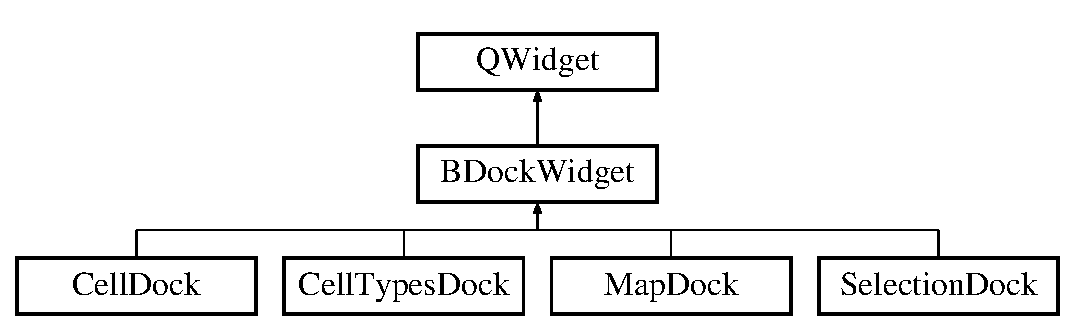
\includegraphics[height=3.000000cm]{class_b_dock_widget}
\end{center}
\end{figure}
\subsection*{Public Slots}
\begin{DoxyCompactItemize}
\item 
\hypertarget{class_b_dock_widget_af5b0bf4f6ccb10d3a6dfb2793dc30fc0}{}\label{class_b_dock_widget_af5b0bf4f6ccb10d3a6dfb2793dc30fc0} 
virtual void {\bfseries update\+Game} ()
\end{DoxyCompactItemize}
\subsection*{Signals}
\begin{DoxyCompactItemize}
\item 
\hypertarget{class_b_dock_widget_aac0c798372f3400d56e974ccbf4b6a2d}{}\label{class_b_dock_widget_aac0c798372f3400d56e974ccbf4b6a2d} 
void {\bfseries game\+Modified} ()
\item 
\hypertarget{class_b_dock_widget_a52d21551cb5aaa800969953d83d5799a}{}\label{class_b_dock_widget_a52d21551cb5aaa800969953d83d5799a} 
void {\bfseries change\+Dock\+Name} (Q\+String)
\end{DoxyCompactItemize}
\subsection*{Public Member Functions}
\begin{DoxyCompactItemize}
\item 
\hypertarget{class_b_dock_widget_ac054be8dfe8c967910190cc31689a2d0}{}\label{class_b_dock_widget_ac054be8dfe8c967910190cc31689a2d0} 
{\bfseries B\+Dock\+Widget} (Q\+Widget $\ast$parent=0)
\item 
\hypertarget{class_b_dock_widget_a47e19ff81c8dbe1fbb6f528bec7bdc2f}{}\label{class_b_dock_widget_a47e19ff81c8dbe1fbb6f528bec7bdc2f} 
void {\bfseries set\+Game} (\hyperlink{class_game}{Game} $\ast$g)
\end{DoxyCompactItemize}
\subsection*{Protected Attributes}
\begin{DoxyCompactItemize}
\item 
\hypertarget{class_b_dock_widget_a2cd159222e09c8034a5ee46628a95fc0}{}\label{class_b_dock_widget_a2cd159222e09c8034a5ee46628a95fc0} 
\hyperlink{class_game}{Game} $\ast$ {\bfseries game}
\end{DoxyCompactItemize}


\subsection{Detailed Description}
The \hyperlink{class_b_dock_widget}{B\+Dock\+Widget} class is the base class for game-\/related docks. 

It provides common functions for set game, update, ... 

The documentation for this class was generated from the following files\+:\begin{DoxyCompactItemize}
\item 
src/editor/\+G\+U\+I/\+Tabs/\+Docks/bdockwidget.\+h\item 
src/editor/\+G\+U\+I/\+Tabs/\+Docks/bdockwidget.\+cpp\end{DoxyCompactItemize}

\hypertarget{class_binary_state_machine}{}\section{Binary\+State\+Machine Class Reference}
\label{class_binary_state_machine}\index{Binary\+State\+Machine@{Binary\+State\+Machine}}


The \hyperlink{class_binary_state_machine}{Binary\+State\+Machine} class is a simple Q\+State\+Machine with two states.  




{\ttfamily \#include $<$intertie.\+h$>$}

Inheritance diagram for Binary\+State\+Machine\+:\begin{figure}[H]
\begin{center}
\leavevmode
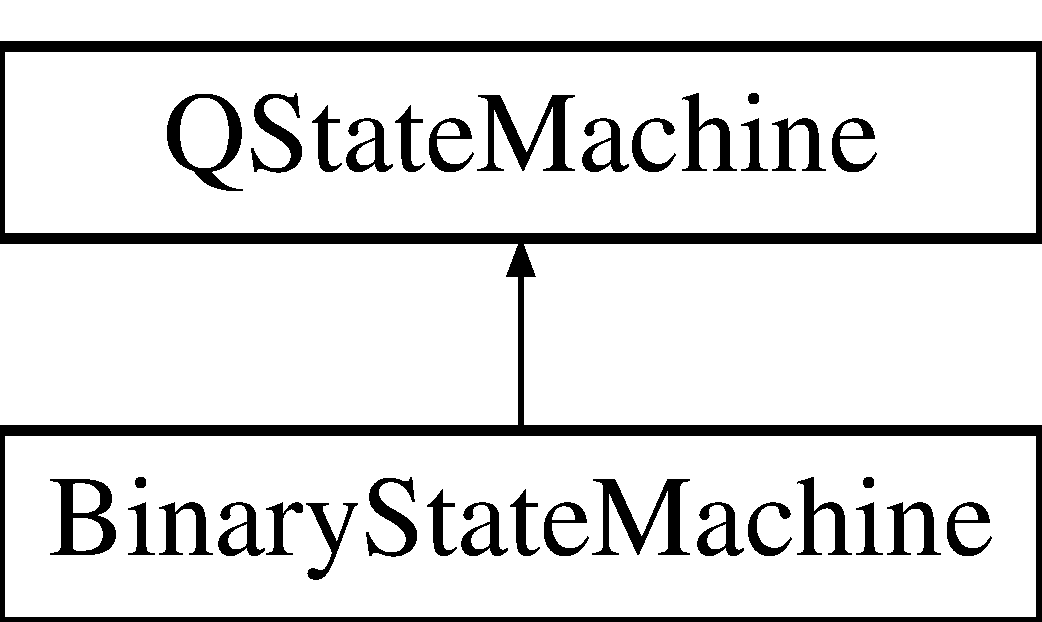
\includegraphics[height=2.000000cm]{class_binary_state_machine}
\end{center}
\end{figure}
\subsection*{Public Slots}
\begin{DoxyCompactItemize}
\item 
\hypertarget{class_binary_state_machine_a797936cea8c62cc1147fdfae5c4668dc}{}\label{class_binary_state_machine_a797936cea8c62cc1147fdfae5c4668dc} 
void {\bfseries swap} ()
\item 
\hypertarget{class_binary_state_machine_a19e75b5bbab7ffd29b18b48f56db1466}{}\label{class_binary_state_machine_a19e75b5bbab7ffd29b18b48f56db1466} 
void {\bfseries set\+Positive} (bool p)
\item 
\hypertarget{class_binary_state_machine_ae3d601827e27a6fa9cac36744c8fe46c}{}\label{class_binary_state_machine_ae3d601827e27a6fa9cac36744c8fe46c} 
void {\bfseries set\+Negative} (bool n)
\end{DoxyCompactItemize}
\subsection*{Signals}
\begin{DoxyCompactItemize}
\item 
\hypertarget{class_binary_state_machine_a2117c089728ebb9b4aa8c1598f655e15}{}\label{class_binary_state_machine_a2117c089728ebb9b4aa8c1598f655e15} 
void {\bfseries swapped} (bool)
\item 
\hypertarget{class_binary_state_machine_adc76e49054c18bfb19de3e2d53da0362}{}\label{class_binary_state_machine_adc76e49054c18bfb19de3e2d53da0362} 
void {\bfseries \+\_\+\+\_\+swap} ()
\end{DoxyCompactItemize}
\subsection*{Public Member Functions}
\begin{DoxyCompactItemize}
\item 
\hypertarget{class_binary_state_machine_a9e022d1bf8c0d7c2c7916c6b329d8891}{}\label{class_binary_state_machine_a9e022d1bf8c0d7c2c7916c6b329d8891} 
{\bfseries Binary\+State\+Machine} (Q\+Object $\ast$parent=0)
\item 
\hypertarget{class_binary_state_machine_a5996c6d83be3422a74e9bf26c30958ca}{}\label{class_binary_state_machine_a5996c6d83be3422a74e9bf26c30958ca} 
void {\bfseries define\+Property} (Q\+Object $\ast$obj, const char $\ast$prop)
\item 
\hypertarget{class_binary_state_machine_a7f9c62ef8512448a2e1afb38f29a7c0f}{}\label{class_binary_state_machine_a7f9c62ef8512448a2e1afb38f29a7c0f} 
void {\bfseries define\+Property} (Q\+Object $\ast$obj, const char $\ast$prop, Q\+Variant yes\+Value, Q\+Variant no\+Value)
\item 
\hypertarget{class_binary_state_machine_ab1279ac5e73d92701a5d0750e23a7048}{}\label{class_binary_state_machine_ab1279ac5e73d92701a5d0750e23a7048} 
bool {\bfseries is\+Positive} () const
\item 
\hypertarget{class_binary_state_machine_a85f770c9351304ec72870970cd7a2e07}{}\label{class_binary_state_machine_a85f770c9351304ec72870970cd7a2e07} 
bool {\bfseries is\+Negative} () const
\end{DoxyCompactItemize}


\subsection{Detailed Description}
The \hyperlink{class_binary_state_machine}{Binary\+State\+Machine} class is a simple Q\+State\+Machine with two states. 

The documentation for this class was generated from the following files\+:\begin{DoxyCompactItemize}
\item 
src/editor/\+G\+U\+I/\+Tabs/\+Docks/intertie.\+h\item 
src/editor/\+G\+U\+I/\+Tabs/\+Docks/intertie.\+cpp\end{DoxyCompactItemize}

\hypertarget{class_b_layout}{\section{\-B\-Layout \-Class \-Reference}
\label{class_b_layout}\index{\-B\-Layout@{\-B\-Layout}}
}


\-The \hyperlink{class_b_layout}{\-B\-Layout} class organise a list of \hyperlink{class_b_dock}{\-B\-Dock} in a widget.  




{\ttfamily \#include $<$bdockszone.\-h$>$}

\subsection*{\-Signals}
\begin{DoxyCompactItemize}
\item 
\hypertarget{class_b_layout_a9e27eb42d23daea4491e31dc65cde9bd}{void {\bfseries size\-Changed} (int)}\label{class_b_layout_a9e27eb42d23daea4491e31dc65cde9bd}

\item 
\hypertarget{class_b_layout_aa9926a76425a6fdc89131feec134444b}{void {\bfseries show\-Point} (int, int)}\label{class_b_layout_aa9926a76425a6fdc89131feec134444b}

\end{DoxyCompactItemize}
\subsection*{\-Public \-Member \-Functions}
\begin{DoxyCompactItemize}
\item 
\hypertarget{class_b_layout_aaa40bac25828f412e0c9f0295143222a}{{\bfseries \-B\-Layout} (\-Q\-Widget $\ast$parent=0)}\label{class_b_layout_aaa40bac25828f412e0c9f0295143222a}

\item 
\hypertarget{class_b_layout_a15af3c6623f5e820b011a237bd896fa5}{void {\bfseries set\-Orientation} (\-Qt\-::\-Orientation o)}\label{class_b_layout_a15af3c6623f5e820b011a237bd896fa5}

\item 
\hypertarget{class_b_layout_ad950c8e9f332986e6367081528de88d6}{void {\bfseries insert} (\hyperlink{class_b_dock}{\-B\-Dock} $\ast$d, int ind=-\/1)}\label{class_b_layout_ad950c8e9f332986e6367081528de88d6}

\item 
\hypertarget{class_b_layout_a2c129fc7bb433119b460eceac0540f85}{void {\bfseries set\-Spacing} (int e)}\label{class_b_layout_a2c129fc7bb433119b460eceac0540f85}

\item 
\hypertarget{class_b_layout_a59a4b4faeeac67c8260f4dd302ff3a66}{void {\bfseries set\-Length} (int t)}\label{class_b_layout_a59a4b4faeeac67c8260f4dd302ff3a66}

\item 
\hypertarget{class_b_layout_ac9a46249e19b37a07f049751df3ef391}{int {\bfseries spacing} () const }\label{class_b_layout_ac9a46249e19b37a07f049751df3ef391}

\end{DoxyCompactItemize}


\subsection{\-Detailed \-Description}
\-The \hyperlink{class_b_layout}{\-B\-Layout} class organise a list of \hyperlink{class_b_dock}{\-B\-Dock} in a widget. 

\-It provides the dock moving functions. 

\-The documentation for this class was generated from the following files\-:\begin{DoxyCompactItemize}
\item 
src/editor/\-G\-U\-I/\-Tabs/\-Docks/\hyperlink{bdockszone_8h}{bdockszone.\-h}\item 
src/editor/\-G\-U\-I/\-Tabs/\-Docks/bdockszone.\-cpp\end{DoxyCompactItemize}

\hypertarget{class_cell}{\section{\-Cell \-Class \-Reference}
\label{class_cell}\index{\-Cell@{\-Cell}}
}


\-The \hyperlink{class_cell}{\-Cell} class.  




{\ttfamily \#include $<$map.\-h$>$}

\-Inheritance diagram for \-Cell\-:\begin{figure}[H]
\begin{center}
\leavevmode
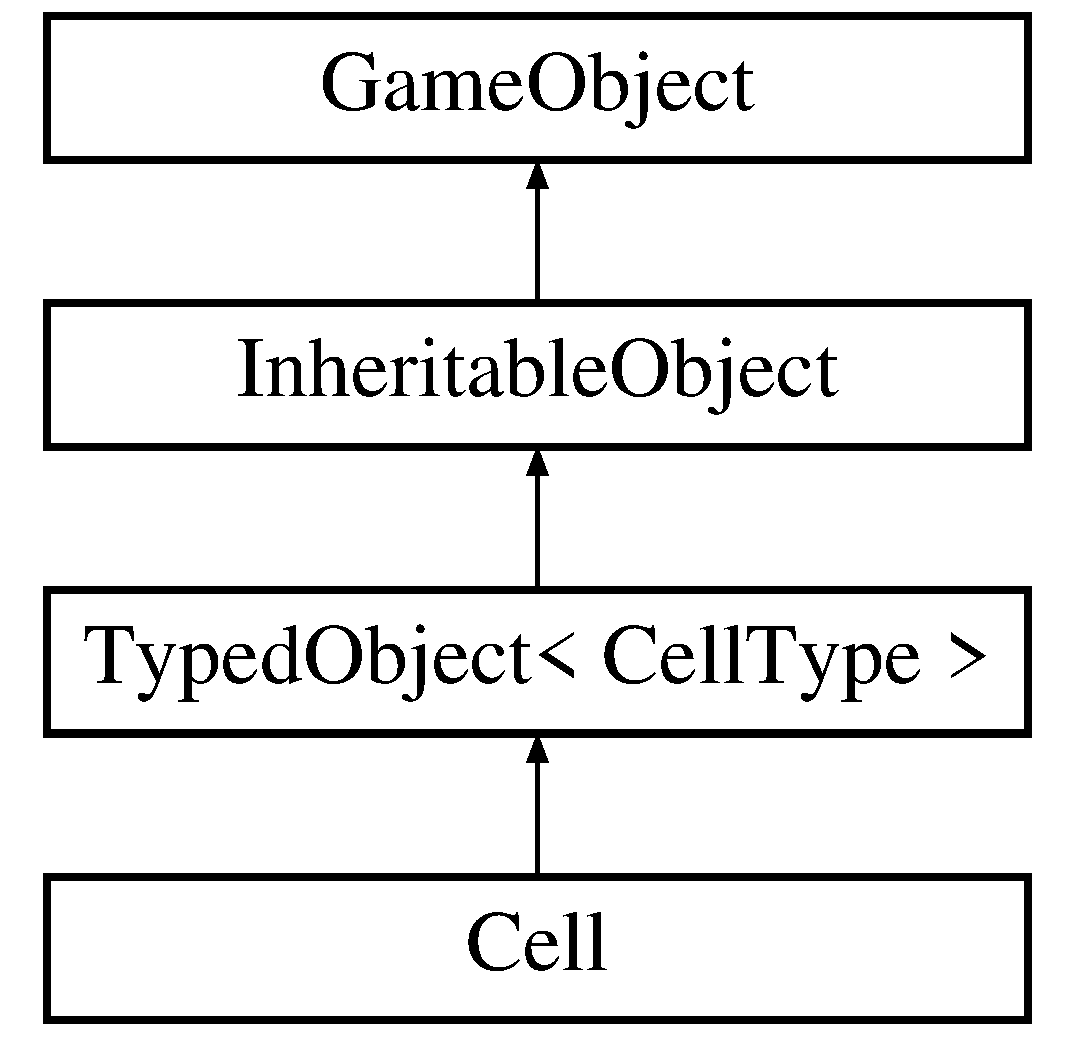
\includegraphics[height=2.000000cm]{class_cell}
\end{center}
\end{figure}
\subsection*{\-Public \-Member \-Functions}
\begin{DoxyCompactItemize}
\item 
\hypertarget{class_cell_ad2edfbf561021e72a464888921c0b576}{{\bfseries \-Cell} (\hyperlink{class_game}{\-Game} $\ast$g=nullptr, \hyperlink{class_game_object}{\-Game\-Object} $\ast$parent=nullptr)}\label{class_cell_ad2edfbf561021e72a464888921c0b576}

\item 
\hypertarget{class_cell_a394830e18401f3b414c3dde4a2b4e2e8}{bool {\bfseries is\-Selected} () const }\label{class_cell_a394830e18401f3b414c3dde4a2b4e2e8}

\item 
\hypertarget{class_cell_a40146bbb2b74cf56337462abc4d0327c}{void {\bfseries set\-Selected} (bool s=true)}\label{class_cell_a40146bbb2b74cf56337462abc4d0327c}

\item 
\hypertarget{class_cell_ad8310bd5ddbdcb3ab3036356556b32b3}{void {\bfseries invert\-Selected} ()}\label{class_cell_ad8310bd5ddbdcb3ab3036356556b32b3}

\item 
\hypertarget{class_cell_a9801c2d435d44834bd14a80fba778618}{void {\bfseries add\-Selection} ()}\label{class_cell_a9801c2d435d44834bd14a80fba778618}

\item 
\hypertarget{class_cell_aa7456089022c5d2dabd4325d03007759}{bool {\bfseries is\-Pre\-Selected} () const }\label{class_cell_aa7456089022c5d2dabd4325d03007759}

\item 
\hypertarget{class_cell_a16f6d41be75c42ad20ad29d0b5725ece}{void {\bfseries confirm\-Pre\-Selection} (bool add=true)}\label{class_cell_a16f6d41be75c42ad20ad29d0b5725ece}

\item 
\hypertarget{class_cell_aa0704872b8d4ae7f40022cfebfa48944}{void {\bfseries clear\-Pre\-Selection} ()}\label{class_cell_aa0704872b8d4ae7f40022cfebfa48944}

\end{DoxyCompactItemize}
\subsection*{\-Data \-Fields}
\begin{DoxyCompactItemize}
\item 
\hypertarget{class_cell_a70f60ede53fb663eb11dd543211bf4cf}{\-Object\-List\-D(o, \-O, bject,, s, \*
\hyperlink{class_object}{\-Object}) private int {\bfseries nb\-Sel}}\label{class_cell_a70f60ede53fb663eb11dd543211bf4cf}

\item 
\hypertarget{class_cell_a5891847674379c2fd25a4d08962a21ba}{bool {\bfseries select\-Mod}}\label{class_cell_a5891847674379c2fd25a4d08962a21ba}

\end{DoxyCompactItemize}


\subsection{\-Detailed \-Description}
\-The \hyperlink{class_cell}{\-Cell} class. 

\-The documentation for this class was generated from the following files\-:\begin{DoxyCompactItemize}
\item 
src/editor/\-Game/\hyperlink{map_8h}{map.\-h}\item 
src/editor/\-Game/map.\-cpp\end{DoxyCompactItemize}

\hypertarget{class_cell_dock}{}\section{Cell\+Dock Class Reference}
\label{class_cell_dock}\index{Cell\+Dock@{Cell\+Dock}}
Inheritance diagram for Cell\+Dock\+:\begin{figure}[H]
\begin{center}
\leavevmode
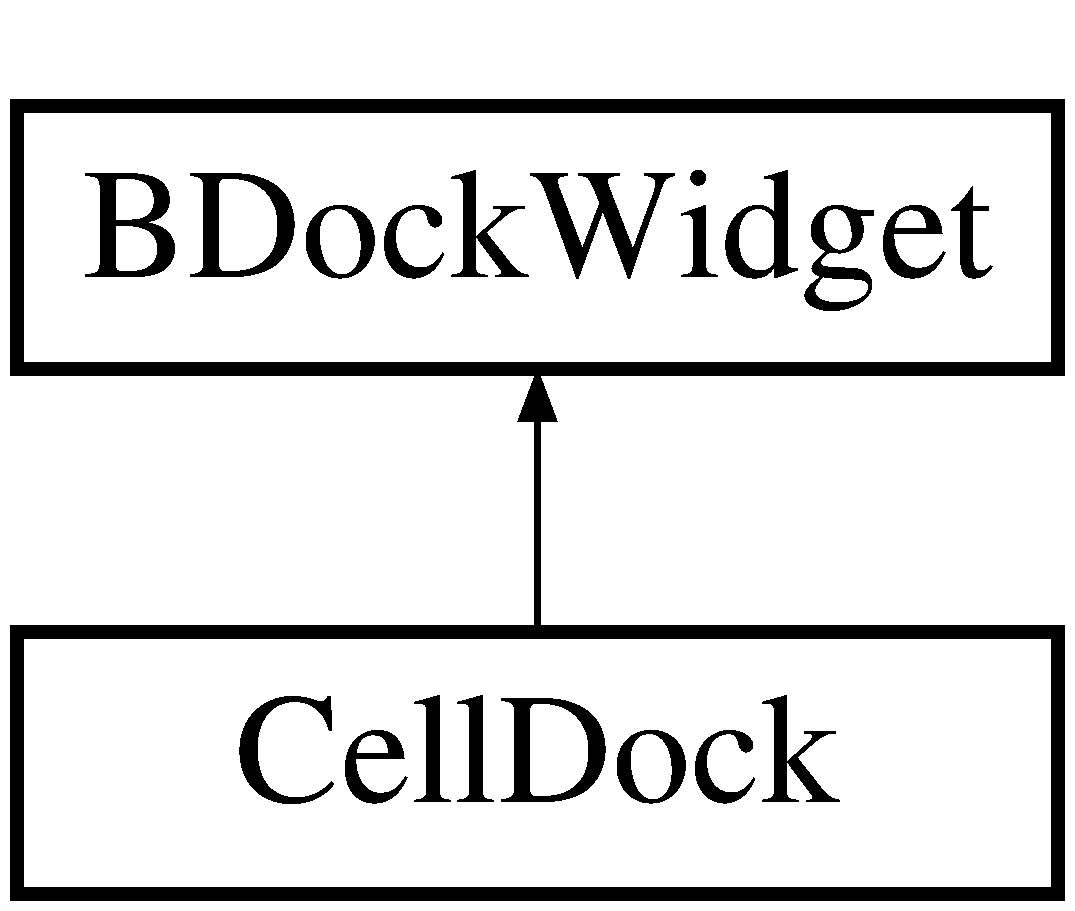
\includegraphics[height=3.000000cm]{class_cell_dock}
\end{center}
\end{figure}
\subsection*{Public Slots}
\begin{DoxyCompactItemize}
\item 
\hypertarget{class_cell_dock_ac33251ff749bac9ec9bc85ae84eefd78}{}\label{class_cell_dock_ac33251ff749bac9ec9bc85ae84eefd78} 
void {\bfseries update\+Game} ()
\item 
\hypertarget{class_cell_dock_aa00bce4b3adaaf6d481f836b2e1a4f53}{}\label{class_cell_dock_aa00bce4b3adaaf6d481f836b2e1a4f53} 
void {\bfseries selection\+Changed} ()
\end{DoxyCompactItemize}
\subsection*{Public Member Functions}
\begin{DoxyCompactItemize}
\item 
\hypertarget{class_cell_dock_a7d5a1e2829fb7c9401a9f3ae7236dde4}{}\label{class_cell_dock_a7d5a1e2829fb7c9401a9f3ae7236dde4} 
{\bfseries Cell\+Dock} (Q\+Widget $\ast$parent=0)
\end{DoxyCompactItemize}
\subsection*{Additional Inherited Members}


The documentation for this class was generated from the following files\+:\begin{DoxyCompactItemize}
\item 
src/editor/\+G\+U\+I/\+Tabs/celldock.\+h\item 
src/editor/\+G\+U\+I/\+Tabs/celldock.\+cpp\end{DoxyCompactItemize}

\hypertarget{class_cell_type}{}\section{Cell\+Type Class Reference}
\label{class_cell_type}\index{Cell\+Type@{Cell\+Type}}


The \hyperlink{class_cell_type}{Cell\+Type} class.  




{\ttfamily \#include $<$map.\+h$>$}

Inheritance diagram for Cell\+Type\+:\begin{figure}[H]
\begin{center}
\leavevmode
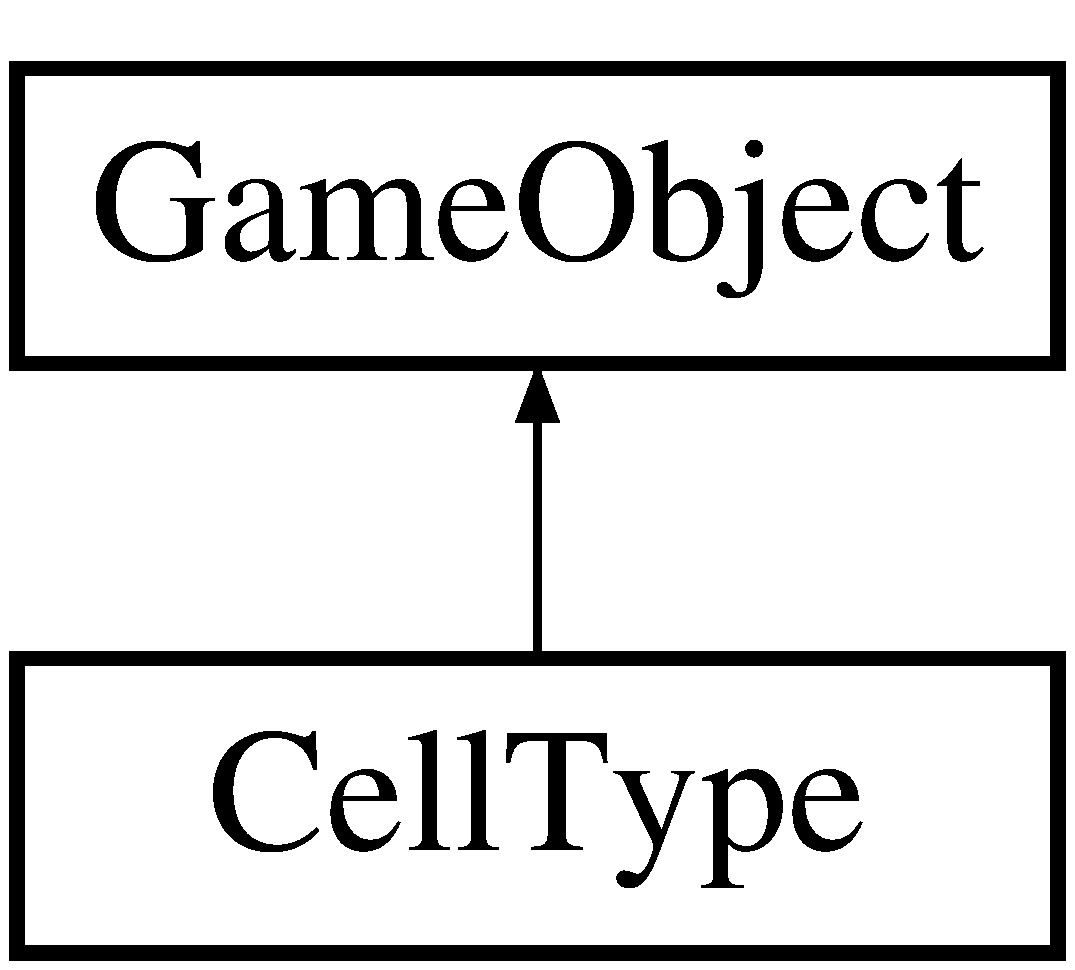
\includegraphics[height=2.000000cm]{class_cell_type}
\end{center}
\end{figure}
\subsection*{Public Member Functions}
\begin{DoxyCompactItemize}
\item 
\hypertarget{class_cell_type_a9764b05a46f0227100874d909ea0e0ce}{}\label{class_cell_type_a9764b05a46f0227100874d909ea0e0ce} 
{\bfseries Cell\+Type} (\hyperlink{class_game}{Game} $\ast$g, \hyperlink{class_game_object}{Game\+Object} $\ast$parent)
\end{DoxyCompactItemize}
\subsection*{Additional Inherited Members}


\subsection{Detailed Description}
The \hyperlink{class_cell_type}{Cell\+Type} class. 

The documentation for this class was generated from the following files\+:\begin{DoxyCompactItemize}
\item 
src/editor/\+Game/\hyperlink{map_8h}{map.\+h}\item 
src/editor/\+Game/map.\+cpp\end{DoxyCompactItemize}

\hypertarget{class_cell_type_editor}{\section{\-Cell\-Type\-Editor \-Class \-Reference}
\label{class_cell_type_editor}\index{\-Cell\-Type\-Editor@{\-Cell\-Type\-Editor}}
}
\subsection*{\-Public \-Member \-Functions}
\begin{DoxyCompactItemize}
\item 
\hypertarget{class_cell_type_editor_a73f1450158ae7ab6db0a030d8ea7602e}{{\bfseries \-Cell\-Type\-Editor} (\-Q\-Widget $\ast$parent=0)}\label{class_cell_type_editor_a73f1450158ae7ab6db0a030d8ea7602e}

\end{DoxyCompactItemize}


\-The documentation for this class was generated from the following files\-:\begin{DoxyCompactItemize}
\item 
src/editor/\-G\-U\-I/\-Tabs/\-Object\-Editors/celltypeeditor.\-h\item 
src/editor/\-G\-U\-I/\-Tabs/\-Object\-Editors/celltypeeditor.\-cpp\end{DoxyCompactItemize}

\hypertarget{class_cell_type_list_model}{\section{\-Cell\-Type\-List\-Model \-Class \-Reference}
\label{class_cell_type_list_model}\index{\-Cell\-Type\-List\-Model@{\-Cell\-Type\-List\-Model}}
}


\-The \hyperlink{class_cell_type_list_model}{\-Cell\-Type\-List\-Model} class.  




{\ttfamily \#include $<$mapslistmodel.\-h$>$}

\subsection*{\-Public \-Member \-Functions}
\begin{DoxyCompactItemize}
\item 
\hypertarget{class_cell_type_list_model_a3e5614c6b52577d4d673ac28e5b19c59}{{\bfseries \-Cell\-Type\-List\-Model} (\hyperlink{class_world}{\-World} $\ast$w, \-Q\-Object $\ast$parent=0)}\label{class_cell_type_list_model_a3e5614c6b52577d4d673ac28e5b19c59}

\item 
\hypertarget{class_cell_type_list_model_a4d19e3ec13380dc4ecfea9ceafdc78b9}{int {\bfseries row\-Count} (const \-Q\-Model\-Index \&parent) const \-Q\-\_\-\-D\-E\-C\-L\-\_\-\-O\-V\-E\-R\-R\-I\-D\-E}\label{class_cell_type_list_model_a4d19e3ec13380dc4ecfea9ceafdc78b9}

\item 
\hypertarget{class_cell_type_list_model_a949e9fd005335e0024fb66f63113078d}{\-Q\-Variant {\bfseries data} (const \-Q\-Model\-Index \&index, int role) const \-Q\-\_\-\-D\-E\-C\-L\-\_\-\-O\-V\-E\-R\-R\-I\-D\-E}\label{class_cell_type_list_model_a949e9fd005335e0024fb66f63113078d}

\item 
\hypertarget{class_cell_type_list_model_aeff00ffac0dd7bce76a505d2eabfed49}{bool {\bfseries insert\-Rows} (int row, int count, const \-Q\-Model\-Index \&parent) \-Q\-\_\-\-D\-E\-C\-L\-\_\-\-O\-V\-E\-R\-R\-I\-D\-E}\label{class_cell_type_list_model_aeff00ffac0dd7bce76a505d2eabfed49}

\item 
\hypertarget{class_cell_type_list_model_abe5727a0615f06531cfa271a607785a4}{bool {\bfseries remove\-Rows} (int row, int count, const \-Q\-Model\-Index \&parent) \-Q\-\_\-\-D\-E\-C\-L\-\_\-\-O\-V\-E\-R\-R\-I\-D\-E}\label{class_cell_type_list_model_abe5727a0615f06531cfa271a607785a4}

\end{DoxyCompactItemize}


\subsection{\-Detailed \-Description}
\-The \hyperlink{class_cell_type_list_model}{\-Cell\-Type\-List\-Model} class. 

\-The documentation for this class was generated from the following files\-:\begin{DoxyCompactItemize}
\item 
src/editor/\-Game/\-Item\-Models/\hyperlink{mapslistmodel_8h}{mapslistmodel.\-h}\item 
src/editor/\-Game/\-Item\-Models/mapslistmodel.\-cpp\end{DoxyCompactItemize}

\hypertarget{class_cell_types_dock}{}\section{Cell\+Types\+Dock Class Reference}
\label{class_cell_types_dock}\index{Cell\+Types\+Dock@{Cell\+Types\+Dock}}
Inheritance diagram for Cell\+Types\+Dock\+:\begin{figure}[H]
\begin{center}
\leavevmode
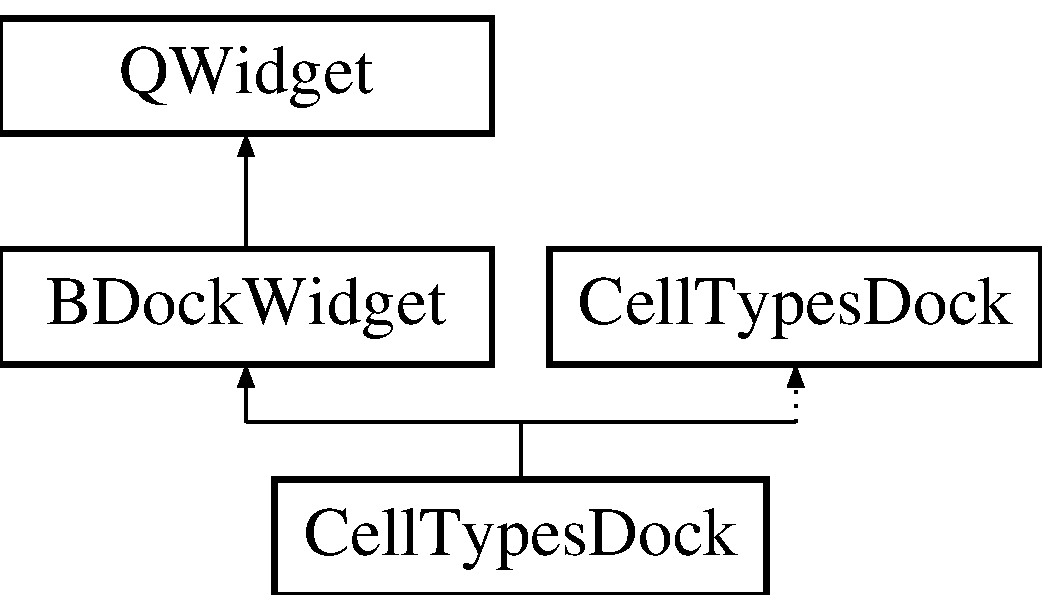
\includegraphics[height=3.000000cm]{class_cell_types_dock}
\end{center}
\end{figure}
\subsection*{Public Member Functions}
\begin{DoxyCompactItemize}
\item 
\hypertarget{class_cell_types_dock_a0e1bc992465cea9c1fc71866b425fcbb}{}\label{class_cell_types_dock_a0e1bc992465cea9c1fc71866b425fcbb} 
{\bfseries Cell\+Types\+Dock} (Q\+Widget $\ast$parent=0)
\item 
\hypertarget{class_cell_types_dock_a700565cc4bb4c3e87d219d4d4726e680}{}\label{class_cell_types_dock_a700565cc4bb4c3e87d219d4d4726e680} 
void {\bfseries update\+Game} ()
\end{DoxyCompactItemize}
\subsection*{Additional Inherited Members}


The documentation for this class was generated from the following files\+:\begin{DoxyCompactItemize}
\item 
src/editor/\+G\+U\+I/\+Tabs/celltypesdock.\+h\item 
src/editor/\+G\+U\+I/\+Tabs/celltypesdock.\+cpp\end{DoxyCompactItemize}

\hypertarget{class_cl_coords}{\section{\-Cl\-Coords \-Class \-Reference}
\label{class_cl_coords}\index{\-Cl\-Coords@{\-Cl\-Coords}}
}


\-The \hyperlink{class_cl_coords}{\-Cl\-Coords} class describe positions with cell coordinates.  




{\ttfamily \#include $<$mappainter.\-h$>$}

\subsection*{\-Public \-Member \-Functions}
\begin{DoxyCompactItemize}
\item 
\hypertarget{class_cl_coords_a45685abe9c81595e2926edc414b425e7}{{\bfseries \-Cl\-Coords} (qreal x, qreal y)}\label{class_cl_coords_a45685abe9c81595e2926edc414b425e7}

\item 
\hypertarget{class_cl_coords_a48c6c4a46561da6e0a14ca6f3483426a}{{\bfseries \-Cl\-Coords} (const \-Q\-Point\-F \&p)}\label{class_cl_coords_a48c6c4a46561da6e0a14ca6f3483426a}

\end{DoxyCompactItemize}


\subsection{\-Detailed \-Description}
\-The \hyperlink{class_cl_coords}{\-Cl\-Coords} class describe positions with cell coordinates. 

\-Theses coordinates describe each point relatively to the cell grid. \-They correspond to the isometric 3\-D world.

\begin{DoxySeeAlso}{\-See also}
\hyperlink{class_rl_coords}{\-Rl\-Coords}, \hyperlink{class_pt_coords}{\-Pt\-Coords}, \hyperlink{class_px_coords}{\-Px\-Coords} 
\end{DoxySeeAlso}


\-The documentation for this class was generated from the following file\-:\begin{DoxyCompactItemize}
\item 
src/editor/\-Game/\hyperlink{mappainter_8h}{mappainter.\-h}\end{DoxyCompactItemize}

\hypertarget{class_default_types}{\section{\-Default\-Types \-Class \-Reference}
\label{class_default_types}\index{\-Default\-Types@{\-Default\-Types}}
}


\-The \hyperlink{class_default_types}{\-Default\-Types} class represents the object that will contains all types.  




{\ttfamily \#include $<$game.\-h$>$}

\-Inheritance diagram for \-Default\-Types\-:\begin{figure}[H]
\begin{center}
\leavevmode
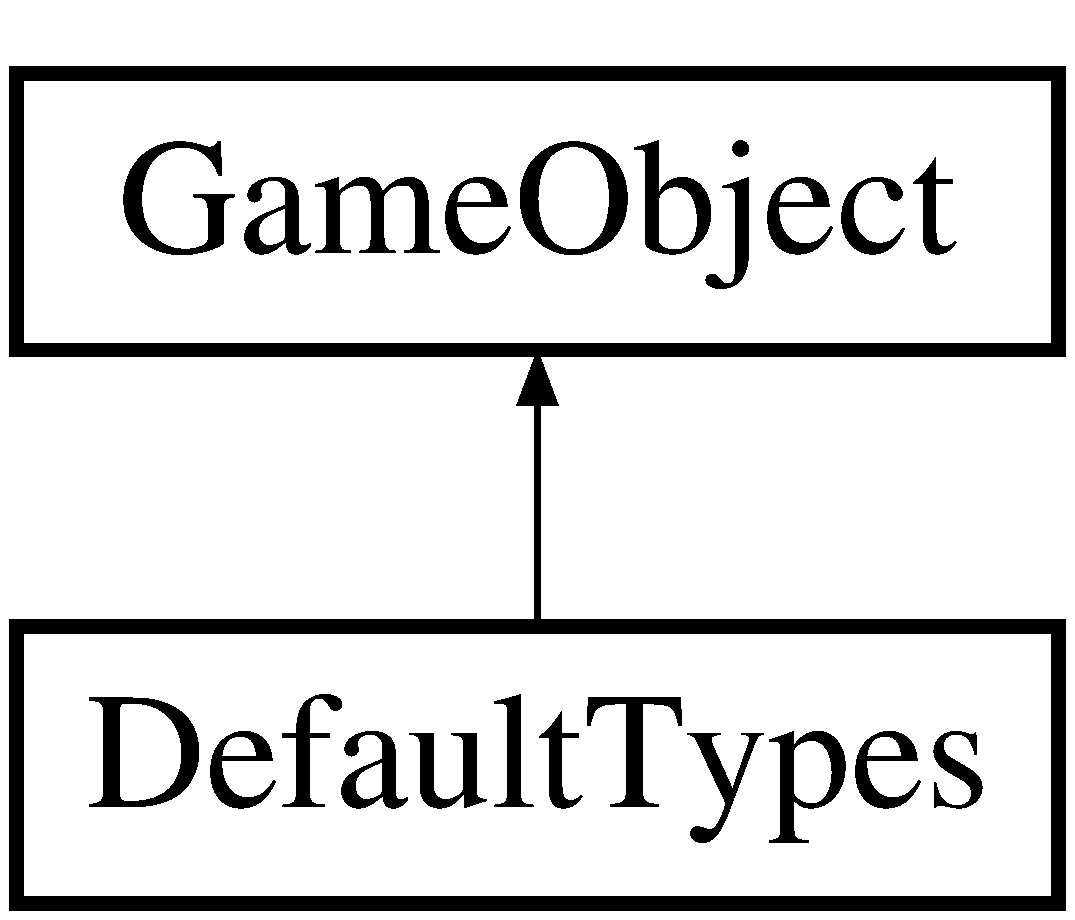
\includegraphics[height=2.000000cm]{class_default_types}
\end{center}
\end{figure}
\subsection*{\-Public \-Member \-Functions}
\begin{DoxyCompactItemize}
\item 
\hypertarget{class_default_types_ae429a10f1aa1c005f0e53dad919b4e44}{\-Types {\bfseries \-Default\-Types} (\hyperlink{class_world}{\-World} \&\hyperlink{class_game_object_af3deaf39cde23c189765634e32e95bb4}{parent})}\label{class_default_types_ae429a10f1aa1c005f0e53dad919b4e44}

\end{DoxyCompactItemize}


\subsection{\-Detailed \-Description}
\-The \hyperlink{class_default_types}{\-Default\-Types} class represents the object that will contains all types. 

\-This \hyperlink{class_default_types}{\-Default\-Types} object has to be given for the construction of the empty type of each type. 

\-The documentation for this class was generated from the following files\-:\begin{DoxyCompactItemize}
\item 
src/editor/\-Game/\hyperlink{game_8h}{game.\-h}\item 
src/editor/\-Game/game.\-cpp\end{DoxyCompactItemize}

\hypertarget{class_editor}{\section{\-Editor \-Class \-Reference}
\label{class_editor}\index{\-Editor@{\-Editor}}
}


\-The \hyperlink{class_editor}{\-Editor} class is the main window of the \hyperlink{class_editor}{\-Editor}.  




{\ttfamily \#include $<$editor.\-h$>$}

\subsection*{\-Public \-Member \-Functions}
\begin{DoxyCompactItemize}
\item 
\hypertarget{class_editor_a7332320d22be46fb91bf0471dac0279b}{{\bfseries \-Editor} (\-Q\-String\-List args, \-Q\-Widget $\ast$parent=0)}\label{class_editor_a7332320d22be46fb91bf0471dac0279b}

\end{DoxyCompactItemize}


\subsection{\-Detailed \-Description}
\-The \hyperlink{class_editor}{\-Editor} class is the main window of the \hyperlink{class_editor}{\-Editor}. 

\-It is composed of tabs that offer editing facilities. 

\-The documentation for this class was generated from the following files\-:\begin{DoxyCompactItemize}
\item 
src/editor/\-G\-U\-I/editor.\-h\item 
src/editor/\-G\-U\-I/editor.\-cpp\end{DoxyCompactItemize}

\hypertarget{class_flag_item_delegate}{\section{\-Flag\-Item\-Delegate \-Class \-Reference}
\label{class_flag_item_delegate}\index{\-Flag\-Item\-Delegate@{\-Flag\-Item\-Delegate}}
}


\-The \hyperlink{class_flag_item_delegate}{\-Flag\-Item\-Delegate} class provides to view classes the way to represent flags and modify them with \-Q\-Check\-Box.  




{\ttfamily \#include $<$itemdelegates.\-h$>$}

\subsection*{\-Public \-Member \-Functions}
\begin{DoxyCompactItemize}
\item 
\hypertarget{class_flag_item_delegate_a886dbd5fb7ed7c7722bdd8586f6f6f4e}{{\bfseries \-Flag\-Item\-Delegate} (\-Q\-Object $\ast$parent=nullptr)}\label{class_flag_item_delegate_a886dbd5fb7ed7c7722bdd8586f6f6f4e}

\item 
\hypertarget{class_flag_item_delegate_ac5e511eb9f27883dc81537b0fd4bb4ba}{\-Q\-Widget $\ast$ {\bfseries create\-Editor} (\-Q\-Widget $\ast$parent, const \-Q\-Style\-Option\-View\-Item \&option, const \-Q\-Model\-Index \&index) const }\label{class_flag_item_delegate_ac5e511eb9f27883dc81537b0fd4bb4ba}

\item 
\hypertarget{class_flag_item_delegate_ad6af4940b2b8ddfa92838b0bf3536992}{void {\bfseries set\-Editor\-Data} (\-Q\-Widget $\ast$editor, const \-Q\-Model\-Index \&index) const }\label{class_flag_item_delegate_ad6af4940b2b8ddfa92838b0bf3536992}

\item 
\hypertarget{class_flag_item_delegate_ad07a72c292304a40b40399b1046185ef}{void {\bfseries update\-Editor\-Geometry} (\-Q\-Widget $\ast$editor, const \-Q\-Style\-Option\-View\-Item \&option, const \-Q\-Model\-Index \&index) const }\label{class_flag_item_delegate_ad07a72c292304a40b40399b1046185ef}

\item 
\hypertarget{class_flag_item_delegate_af09a6555dc565638f142075c68da7134}{void {\bfseries set\-Model\-Data} (\-Q\-Widget $\ast$editor, \-Q\-Abstract\-Item\-Model $\ast$model, const \-Q\-Model\-Index \&index) const }\label{class_flag_item_delegate_af09a6555dc565638f142075c68da7134}

\item 
\hypertarget{class_flag_item_delegate_a899335352d13ca510da90d4ef285e313}{void {\bfseries paint} (\-Q\-Painter $\ast$painter, const \-Q\-Style\-Option\-View\-Item \&option, const \-Q\-Model\-Index \&index) const }\label{class_flag_item_delegate_a899335352d13ca510da90d4ef285e313}

\end{DoxyCompactItemize}


\subsection{\-Detailed \-Description}
\-The \hyperlink{class_flag_item_delegate}{\-Flag\-Item\-Delegate} class provides to view classes the way to represent flags and modify them with \-Q\-Check\-Box. 

\begin{DoxySeeAlso}{\-See also}
\hyperlink{class_param_item_delegate}{\-Param\-Item\-Delegate} 
\end{DoxySeeAlso}


\-The documentation for this class was generated from the following files\-:\begin{DoxyCompactItemize}
\item 
src/editor/\-G\-U\-I/\-Tabs/\hyperlink{itemdelegates_8h}{itemdelegates.\-h}\item 
src/editor/\-G\-U\-I/\-Tabs/itemdelegates.\-cpp\end{DoxyCompactItemize}

\hypertarget{class_flag_tree_item_model}{\section{\-Flag\-Tree\-Item\-Model \-Class \-Reference}
\label{class_flag_tree_item_model}\index{\-Flag\-Tree\-Item\-Model@{\-Flag\-Tree\-Item\-Model}}
}


\-The \hyperlink{class_param_tree_item_model}{\-Param\-Tree\-Item\-Model} class presents the flags of an object using the \-Q\-Abstract\-Item\-Model interface.  




{\ttfamily \#include $<$attrtreeitemmodel.\-h$>$}

\subsection*{\-Public \-Member \-Functions}
\begin{DoxyCompactItemize}
\item 
\hypertarget{class_flag_tree_item_model_af0dbdaefea99e8bf0ccf247b7d99a3b9}{{\bfseries \-Flag\-Tree\-Item\-Model} (\-Q\-Object $\ast$parent=0)}\label{class_flag_tree_item_model_af0dbdaefea99e8bf0ccf247b7d99a3b9}

\item 
\hypertarget{class_flag_tree_item_model_af65b7aa347352ec15c648b922dd358ef}{void {\bfseries set\-Object} (\hyperlink{class_game_object}{\-Game\-Object} $\ast$o)}\label{class_flag_tree_item_model_af65b7aa347352ec15c648b922dd358ef}

\item 
\hypertarget{class_flag_tree_item_model_ad6a00e5fca9bd0b9ade572e2511f8401}{int {\bfseries column\-Count} (const \-Q\-Model\-Index \&parent) const }\label{class_flag_tree_item_model_ad6a00e5fca9bd0b9ade572e2511f8401}

\item 
\hypertarget{class_flag_tree_item_model_a997e3c0716e844a05b25d73e94db3808}{int {\bfseries row\-Count} (const \-Q\-Model\-Index \&parent) const }\label{class_flag_tree_item_model_a997e3c0716e844a05b25d73e94db3808}

\item 
\hypertarget{class_flag_tree_item_model_aa427bd54c7dbbff91243f9b3881c45ed}{\-Qt\-::\-Item\-Flags {\bfseries flags} (const \-Q\-Model\-Index \&index) const }\label{class_flag_tree_item_model_aa427bd54c7dbbff91243f9b3881c45ed}

\item 
\hypertarget{class_flag_tree_item_model_aaa1f651be87a4ea92da6bb80ed45b461}{\-Q\-Variant {\bfseries data} (const \-Q\-Model\-Index \&index, int role) const }\label{class_flag_tree_item_model_aaa1f651be87a4ea92da6bb80ed45b461}

\item 
\hypertarget{class_flag_tree_item_model_a140ab0b93de0c70e73981ef7d70dcf56}{\-Q\-Model\-Index {\bfseries index} (int row, int column, const \-Q\-Model\-Index \&parent) const }\label{class_flag_tree_item_model_a140ab0b93de0c70e73981ef7d70dcf56}

\item 
\hypertarget{class_flag_tree_item_model_ae6eefe6171c2aee060ec8d39403021ce}{\-Q\-Model\-Index {\bfseries parent} (const \-Q\-Model\-Index \&child) const }\label{class_flag_tree_item_model_ae6eefe6171c2aee060ec8d39403021ce}

\item 
\hypertarget{class_flag_tree_item_model_a8dbb4bf08c8dd4f63f5cf448dfaa4862}{\-Q\-Variant {\bfseries header\-Data} (int section, \-Qt\-::\-Orientation orientation, int role) const }\label{class_flag_tree_item_model_a8dbb4bf08c8dd4f63f5cf448dfaa4862}

\item 
\hypertarget{class_flag_tree_item_model_a574c890e9ccf9575b362d88d2bd7a36c}{bool {\bfseries set\-Data} (const \-Q\-Model\-Index \&index, const \-Q\-Variant \&value, int role)}\label{class_flag_tree_item_model_a574c890e9ccf9575b362d88d2bd7a36c}

\item 
\hypertarget{class_flag_tree_item_model_a51ff995bbfb7c54d608ec23205280211}{void {\bfseries add\-Flag} (const \-Q\-String \&name)}\label{class_flag_tree_item_model_a51ff995bbfb7c54d608ec23205280211}

\item 
\hypertarget{class_flag_tree_item_model_a41730252f38ebda9c249a615ab5b2af2}{void {\bfseries sort\-Attr} (const \-Q\-Model\-Index \&par)}\label{class_flag_tree_item_model_a41730252f38ebda9c249a615ab5b2af2}

\end{DoxyCompactItemize}


\subsection{\-Detailed \-Description}
\-The \hyperlink{class_param_tree_item_model}{\-Param\-Tree\-Item\-Model} class presents the flags of an object using the \-Q\-Abstract\-Item\-Model interface. 

\begin{DoxySeeAlso}{\-See also}
\hyperlink{class_param_tree_item_model}{\-Param\-Tree\-Item\-Model}, \hyperlink{class_event_tree_item_model}{\-Event\-Tree\-Item\-Model}, \hyperlink{class_order_tree_item_model}{\-Order\-Tree\-Item\-Model} 
\end{DoxySeeAlso}


\-The documentation for this class was generated from the following files\-:\begin{DoxyCompactItemize}
\item 
src/editor/\-Game/\-Item\-Models/\hyperlink{attrtreeitemmodel_8h}{attrtreeitemmodel.\-h}\item 
src/editor/\-Game/\-Item\-Models/attrtreeitemmodel.\-cpp\end{DoxyCompactItemize}

\hypertarget{class_flag_tree_view}{\section{\-Flag\-Tree\-View \-Class \-Reference}
\label{class_flag_tree_view}\index{\-Flag\-Tree\-View@{\-Flag\-Tree\-View}}
}


\-The \hyperlink{class_flag_tree_view}{\-Flag\-Tree\-View} class customize \-Qt \-Q\-Tree\-View class to render \hyperlink{class_flag_tree_item_model}{\-Flag\-Tree\-Item\-Model}.  




{\ttfamily \#include $<$treeviews.\-h$>$}

\subsection*{\-Public \-Member \-Functions}
\begin{DoxyCompactItemize}
\item 
\hypertarget{class_flag_tree_view_a86985ac668579405a7f48cb907f1f531}{{\bfseries \-Flag\-Tree\-View} (\-Q\-Widget $\ast$parent=nullptr)}\label{class_flag_tree_view_a86985ac668579405a7f48cb907f1f531}

\item 
\hypertarget{class_flag_tree_view_a9e83c94c3b971d01275c747ad30003ee}{void {\bfseries expand\-View} (const \-Q\-Model\-Index \&index=\-Q\-Model\-Index())}\label{class_flag_tree_view_a9e83c94c3b971d01275c747ad30003ee}

\end{DoxyCompactItemize}


\subsection{\-Detailed \-Description}
\-The \hyperlink{class_flag_tree_view}{\-Flag\-Tree\-View} class customize \-Qt \-Q\-Tree\-View class to render \hyperlink{class_flag_tree_item_model}{\-Flag\-Tree\-Item\-Model}. 

\-The documentation for this class was generated from the following files\-:\begin{DoxyCompactItemize}
\item 
src/editor/\-G\-U\-I/\-Tabs/\hyperlink{treeviews_8h}{treeviews.\-h}\item 
src/editor/\-G\-U\-I/\-Tabs/treeviews.\-cpp\end{DoxyCompactItemize}

\hypertarget{class_game}{\section{\-Game \-Class \-Reference}
\label{class_game}\index{\-Game@{\-Game}}
}


\-The \hyperlink{class_game}{\-Game} class gather the differents parts needed to describe a game.  




{\ttfamily \#include $<$game.\-h$>$}

\-Inheritance diagram for \-Game\-:\begin{figure}[H]
\begin{center}
\leavevmode
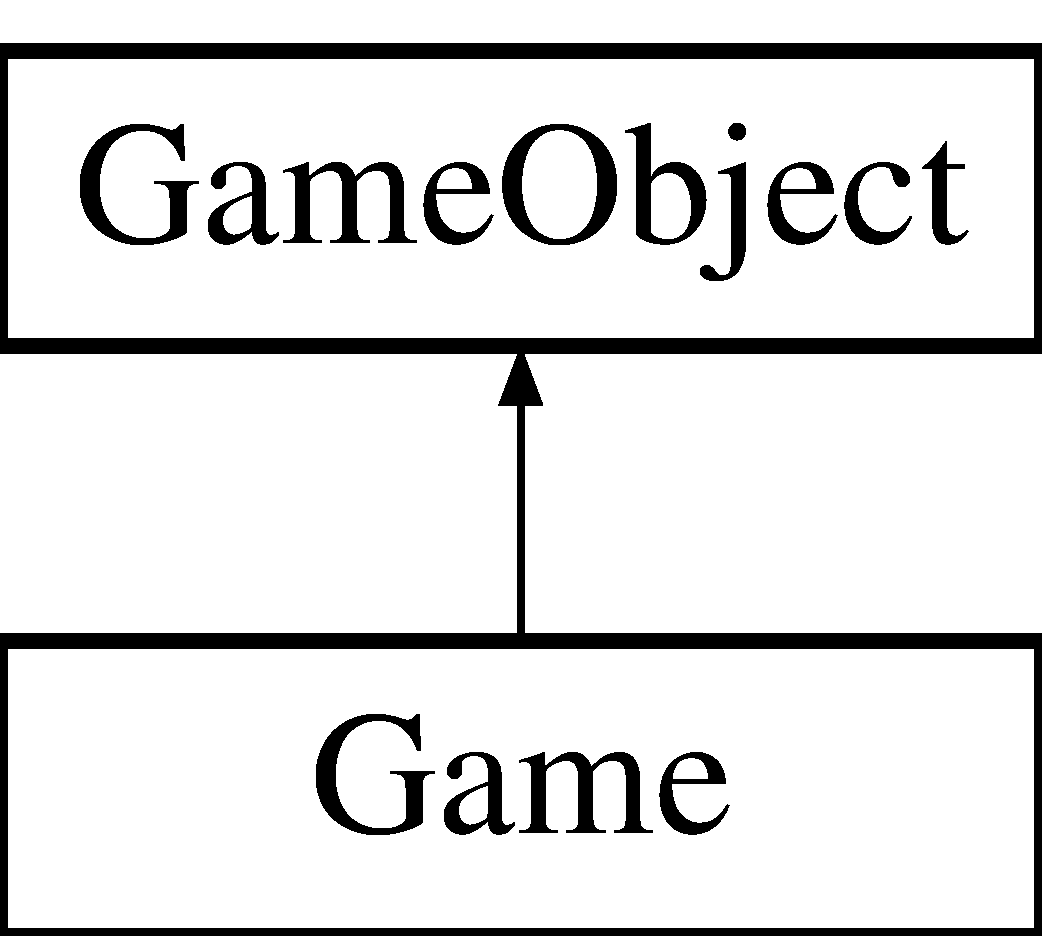
\includegraphics[height=2.000000cm]{class_game}
\end{center}
\end{figure}
\subsection*{\-Public \-Member \-Functions}
\begin{DoxyCompactItemize}
\item 
\hypertarget{class_game_a8df2d5e5d28872b8a1d275d1ca92be4a}{{\bfseries \-Type\-Name} (\hyperlink{class_game}{\-Game}) \hyperlink{class_game}{\-Game}()}\label{class_game_a8df2d5e5d28872b8a1d275d1ca92be4a}

\item 
int \hyperlink{class_game_aeed0ba100700fb2f5d701fcf14d8871e}{new\-Ident} ()
\item 
\hypertarget{class_game_a38feaf6c233d25c2ad353bab65559790}{\hyperlink{class_world}{\-World} $\ast$ {\bfseries world} ()}\label{class_game_a38feaf6c233d25c2ad353bab65559790}

\item 
\hypertarget{class_game_a3b242dcb7703b409692ce0c91e799a8c}{\hyperlink{class_map}{\-Map} $\ast$ {\bfseries current\-Map} ()}\label{class_game_a3b242dcb7703b409692ce0c91e799a8c}

\item 
\hypertarget{class_game_af7394ea8ff98b0b819125a6bac47db2b}{void {\bfseries set\-Current\-Map} (\hyperlink{class_map}{\-Map} $\ast$m)}\label{class_game_af7394ea8ff98b0b819125a6bac47db2b}

\item 
\hypertarget{class_game_a8c246c639e16c351b7f261dc44a0897d}{void {\bfseries add\-Image} (\hyperlink{class_image}{\-Image} $\ast$im)}\label{class_game_a8c246c639e16c351b7f261dc44a0897d}

\end{DoxyCompactItemize}


\subsection{\-Detailed \-Description}
\-The \hyperlink{class_game}{\-Game} class gather the differents parts needed to describe a game. 

\-It contains mainly the \hyperlink{class_world}{\-World}, and the ressources used by it (images and strings)

\-For editing purposes, it contains also the active map (the one being editing) 

\subsection{\-Member \-Function \-Documentation}
\hypertarget{class_game_aeed0ba100700fb2f5d701fcf14d8871e}{\index{\-Game@{\-Game}!new\-Ident@{new\-Ident}}
\index{new\-Ident@{new\-Ident}!Game@{\-Game}}
\subsubsection[{new\-Ident}]{\setlength{\rightskip}{0pt plus 5cm}int {\bf \-Game\-::new\-Ident} (
\begin{DoxyParamCaption}
{}
\end{DoxyParamCaption}
)\hspace{0.3cm}{\ttfamily  \mbox{[}inline\mbox{]}}}}\label{class_game_aeed0ba100700fb2f5d701fcf14d8871e}
\-Returns a new unused identifiers

\begin{DoxyNote}{\-Note}
\-It should only be used by \hyperlink{class_game_object}{\-Game\-Object} methods \hyperlink{class_game_object_a97be7b59b2e76e7d60de2146b894eed9}{\-Game\-Object\-::init} and \-Game\-Object\-::\-Game\-Object. 
\end{DoxyNote}


\-The documentation for this class was generated from the following files\-:\begin{DoxyCompactItemize}
\item 
src/editor/\-Game/\hyperlink{game_8h}{game.\-h}\item 
src/editor/\-Game/game.\-cpp\end{DoxyCompactItemize}

\hypertarget{class_game_object}{\section{\-Game\-Object \-Class \-Reference}
\label{class_game_object}\index{\-Game\-Object@{\-Game\-Object}}
}


\-The \hyperlink{class_game_object}{\-Game\-Object} class is the base class for every part of games.  




{\ttfamily \#include $<$object.\-h$>$}

\-Inheritance diagram for \-Game\-Object\-:\begin{figure}[H]
\begin{center}
\leavevmode
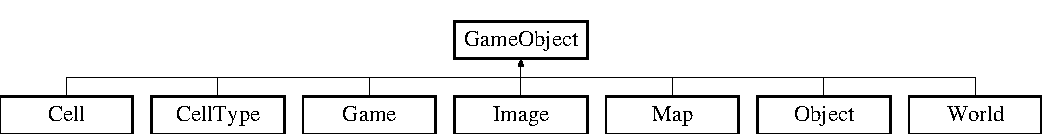
\includegraphics[height=1.797753cm]{class_game_object}
\end{center}
\end{figure}
\subsection*{\-Public \-Member \-Functions}
\begin{DoxyCompactItemize}
\item 
\hyperlink{class_game_object_ab00c537faf6eb4439c60003141a763b9}{\-Game\-Object} (\hyperlink{class_game}{\-Game} $\ast$g=nullptr, \hyperlink{class_game_object}{\-Game\-Object} $\ast$parent=nullptr)
\item 
void \hyperlink{class_game_object_a97be7b59b2e76e7d60de2146b894eed9}{init} (\hyperlink{class_game}{\-Game} $\ast$g, \hyperlink{class_game_object}{\-Game\-Object} $\ast$p)
\item 
virtual bool \hyperlink{class_game_object_a88676a10f8e905747f1d64c2da490524}{is\-Valid} () const 
\item 
int \hyperlink{class_game_object_a4d84063c56c17bfdee8844eb3fa3445a}{ident} () const 
\item 
const \-Q\-Date\-Time \& \hyperlink{class_game_object_a0c4cc65819b30ec36a1c20a1c24997fe}{last\-Internal\-Edition} () const 
\item 
const \-Q\-Date\-Time \& \hyperlink{class_game_object_acc65ad08191fcaf558bd1840a45d23cf}{last\-Children\-Edition} () const 
\item 
const \-Q\-Date\-Time \& \hyperlink{class_game_object_a73b351287147712a937e87028bf8c876}{last\-Edition} () const 
\item 
int \hyperlink{class_game_object_a27de46b2b9b439755b1e57df51c35caf}{get\-Param} (const \-Q\-String \&p) const 
\item 
void \hyperlink{class_game_object_a28b8af7f399f1348a4f3130dd21173a1}{set\-Param} (const \-Q\-String \&p, int v)
\item 
bool \hyperlink{class_game_object_aa48c29e1ac9e9289f4647f8e263b9fae}{has\-Param} (const \-Q\-String \&p) const 
\item 
\-Q\-List$<$ \-Q\-String $>$ \hyperlink{class_game_object_a3e851f9aceb9e868a73dd58fe8e3719f}{params} () const 
\item 
bool \hyperlink{class_game_object_a30bc22a11619930d442bc16f0c938339}{get\-Flag} (const \-Q\-String \&f) const 
\item 
void \hyperlink{class_game_object_ae7984096fc518b15c0b080c543e4c42f}{set\-Flag} (const \-Q\-String \&f, bool v)
\item 
bool \hyperlink{class_game_object_a3c4f7121e75a8340a32e20f16b63b412}{has\-Flag} (const \-Q\-String \&f) const 
\item 
\-Q\-List$<$ \-Q\-String $>$ \hyperlink{class_game_object_aa9a0d6ea1bd41e4d4a370d2f010ac533}{flags} () const 
\item 
void \hyperlink{class_game_object_a2130d5674df041b5a7eaf987f9b1e642}{touch} ()
\item 
\hypertarget{class_game_object_a815c7f587c0ae528614add95655d9a0a}{void {\bfseries add\-Reference} ()}\label{class_game_object_a815c7f587c0ae528614add95655d9a0a}

\item 
\hypertarget{class_game_object_a68725fd75f55bc73bb44216406ce34e5}{void {\bfseries remove\-Reference} ()}\label{class_game_object_a68725fd75f55bc73bb44216406ce34e5}

\item 
\hypertarget{class_game_object_ae34944b23d5d7d472d5c8da3f42fb2e3}{void {\bfseries set\-Parent} (\hyperlink{class_game_object}{\-Game\-Object} $\ast$p)}\label{class_game_object_ae34944b23d5d7d472d5c8da3f42fb2e3}

\end{DoxyCompactItemize}
\subsection*{\-Protected \-Member \-Functions}
\begin{DoxyCompactItemize}
\item 
\hypertarget{class_game_object_a4733a1081db3c2d0a9be225265283ad8}{void {\bfseries add\-Child} (\hyperlink{class_game_object}{\-Game\-Object} $\ast$c)}\label{class_game_object_a4733a1081db3c2d0a9be225265283ad8}

\item 
\hypertarget{class_game_object_a21dc679cb474b147b7d7d336117ffe58}{void {\bfseries remove\-Child} (\hyperlink{class_game_object}{\-Game\-Object} $\ast$c)}\label{class_game_object_a21dc679cb474b147b7d7d336117ffe58}

\item 
\hypertarget{class_game_object_a4e57d5a3f8be6882e5d7f2a2e5d45ccd}{void {\bfseries children\-Touched} (const \-Q\-Date\-Time \&d)}\label{class_game_object_a4e57d5a3f8be6882e5d7f2a2e5d45ccd}

\end{DoxyCompactItemize}
\subsection*{\-Protected \-Attributes}
\begin{DoxyCompactItemize}
\item 
\hypertarget{class_game_object_a4113a496ed45ca90756cfa0d8dfe6171}{\hyperlink{class_game_object}{\-Game\-Object} $\ast$ {\bfseries parent}}\label{class_game_object_a4113a496ed45ca90756cfa0d8dfe6171}

\item 
\hypertarget{class_game_object_a096e6989277570032586b162e5802181}{\-Q\-Map$<$ int, \hyperlink{class_game_object}{\-Game\-Object} $\ast$ $>$ {\bfseries children}}\label{class_game_object_a096e6989277570032586b162e5802181}

\item 
\hypertarget{class_game_object_a338ed91d0ad6aebe8a8d3adf8c75752b}{\hyperlink{class_game}{\-Game} $\ast$ {\bfseries game}}\label{class_game_object_a338ed91d0ad6aebe8a8d3adf8c75752b}

\item 
\hypertarget{class_game_object_a98291c60da12d9036e1ad24cfebcf6b3}{int {\bfseries id}}\label{class_game_object_a98291c60da12d9036e1ad24cfebcf6b3}

\item 
\hypertarget{class_game_object_a1873810f18db1e1faecc04e0ab92c512}{int {\bfseries nb\-Ref}}\label{class_game_object_a1873810f18db1e1faecc04e0ab92c512}

\item 
\hypertarget{class_game_object_ab5ed36754a777ef648dd6831c0b1d6fb}{\-Q\-Map$<$ \-Q\-String, int $>$ {\bfseries a\-Params}}\label{class_game_object_ab5ed36754a777ef648dd6831c0b1d6fb}

\item 
\hypertarget{class_game_object_ade46e4f590a01cab331d12d0da644625}{\-Q\-Map$<$ \-Q\-String, bool $>$ {\bfseries a\-Flags}}\label{class_game_object_ade46e4f590a01cab331d12d0da644625}

\item 
\hypertarget{class_game_object_a8e62a0d6755b2930090348622f482f6d}{\-Q\-String {\bfseries file\-Name}}\label{class_game_object_a8e62a0d6755b2930090348622f482f6d}

\item 
\hypertarget{class_game_object_ac1a61f57d5a318b86c4f2bbb4dbde78f}{\-Q\-Date\-Time {\bfseries last\-Edit}}\label{class_game_object_ac1a61f57d5a318b86c4f2bbb4dbde78f}

\item 
\hypertarget{class_game_object_ae0a43c76fc9171015b43d008b5ffcbfd}{\-Q\-Date\-Time {\bfseries last\-Child\-Edit}}\label{class_game_object_ae0a43c76fc9171015b43d008b5ffcbfd}

\end{DoxyCompactItemize}


\subsection{\-Detailed \-Description}
\-The \hyperlink{class_game_object}{\-Game\-Object} class is the base class for every part of games. 

\-Each instance is identified by a game-\/wide unique identifier.

\#\# \-Object edition notification mechanism

\-To make the edition easier, each \hyperlink{class_game_object}{\-Game\-Object} contains two \-Q\-Date\-Time values \-:
\begin{DoxyItemize}
\item \-The most recent edition time, which is updated by the \hyperlink{class_game_object_a2130d5674df041b5a7eaf987f9b1e642}{touch} method
\item \-The most recent chidl edition time, also updated by the \hyperlink{class_game_object_a2130d5674df041b5a7eaf987f9b1e642}{touch} method
\end{DoxyItemize}

\begin{DoxyNote}{\-Note}
\-If the changes that are made in the object have to be detected by display/edition widgets, the \hyperlink{class_game_object_a2130d5674df041b5a7eaf987f9b1e642}{touch} function should be called. 

\-To prevent the notification chain to be broken, the existing objects should always have a parent (except for the root object). \-This can be acheived using the \hyperlink{class_game_object_a97be7b59b2e76e7d60de2146b894eed9}{init} or set\-Parent method, when the parent have not been given in the constructor. (see \hyperlink{object_8h}{object.\-h} for details)
\end{DoxyNote}
\#\# \-References count

\begin{DoxyRefDesc}{\-Todo}
\item[\hyperlink{todo__todo000001}{\-Todo}]\end{DoxyRefDesc}


\subsection{\-Constructor \& \-Destructor \-Documentation}
\hypertarget{class_game_object_ab00c537faf6eb4439c60003141a763b9}{\index{\-Game\-Object@{\-Game\-Object}!\-Game\-Object@{\-Game\-Object}}
\index{\-Game\-Object@{\-Game\-Object}!GameObject@{\-Game\-Object}}
\subsubsection[{\-Game\-Object}]{\setlength{\rightskip}{0pt plus 5cm}{\bf \-Game\-Object\-::\-Game\-Object} (
\begin{DoxyParamCaption}
\item[{{\bf \-Game} $\ast$}]{g = {\ttfamily nullptr}, }
\item[{{\bf \-Game\-Object} $\ast$}]{parent = {\ttfamily nullptr}}
\end{DoxyParamCaption}
)}}\label{class_game_object_ab00c537faf6eb4439c60003141a763b9}
\-Constructs a new \hyperlink{class_game_object}{\-Game\-Object} with parent {\ttfamily parent} and the reference to the game {\ttfamily g}.

\begin{DoxyNote}{\-Note}
\-If these objects cannot be given to the constructor (case of an array of objects), the \hyperlink{class_game_object_a97be7b59b2e76e7d60de2146b894eed9}{init} method must be called after the creation to make the \hyperlink{class_game_object}{\-Game\-Object} valid. 
\end{DoxyNote}


\subsection{\-Member \-Function \-Documentation}
\hypertarget{class_game_object_aa9a0d6ea1bd41e4d4a370d2f010ac533}{\index{\-Game\-Object@{\-Game\-Object}!flags@{flags}}
\index{flags@{flags}!GameObject@{\-Game\-Object}}
\subsubsection[{flags}]{\setlength{\rightskip}{0pt plus 5cm}\-Q\-List$<$\-Q\-String$>$ {\bf \-Game\-Object\-::flags} (
\begin{DoxyParamCaption}
{}
\end{DoxyParamCaption}
) const\hspace{0.3cm}{\ttfamily  \mbox{[}inline\mbox{]}}}}\label{class_game_object_aa9a0d6ea1bd41e4d4a370d2f010ac533}
\-Returns the list of the registered flags

\begin{DoxySeeAlso}{\-See also}
\hyperlink{class_game_object_a30bc22a11619930d442bc16f0c938339}{get\-Flag}, \hyperlink{class_game_object_ae7984096fc518b15c0b080c543e4c42f}{set\-Flag}, \hyperlink{class_game_object_a3e851f9aceb9e868a73dd58fe8e3719f}{params} 
\end{DoxySeeAlso}
\hypertarget{class_game_object_a30bc22a11619930d442bc16f0c938339}{\index{\-Game\-Object@{\-Game\-Object}!get\-Flag@{get\-Flag}}
\index{get\-Flag@{get\-Flag}!GameObject@{\-Game\-Object}}
\subsubsection[{get\-Flag}]{\setlength{\rightskip}{0pt plus 5cm}bool {\bf \-Game\-Object\-::get\-Flag} (
\begin{DoxyParamCaption}
\item[{const \-Q\-String \&}]{f}
\end{DoxyParamCaption}
) const\hspace{0.3cm}{\ttfamily  \mbox{[}inline\mbox{]}}}}\label{class_game_object_a30bc22a11619930d442bc16f0c938339}
\-Returns the value of the {\ttfamily f} flag.

\begin{DoxyNote}{\-Note}
\-If the requested parameter does not exists, a {\ttfamily false} value is returned, and the flags map stay unchanged
\end{DoxyNote}
\begin{DoxySeeAlso}{\-See also}
\hyperlink{class_game_object_aa9a0d6ea1bd41e4d4a370d2f010ac533}{flags}, \hyperlink{class_game_object_a3c4f7121e75a8340a32e20f16b63b412}{has\-Flag}, \hyperlink{class_game_object_ae7984096fc518b15c0b080c543e4c42f}{set\-Flag}, \hyperlink{class_game_object_a27de46b2b9b439755b1e57df51c35caf}{get\-Param} 
\end{DoxySeeAlso}
\hypertarget{class_game_object_a27de46b2b9b439755b1e57df51c35caf}{\index{\-Game\-Object@{\-Game\-Object}!get\-Param@{get\-Param}}
\index{get\-Param@{get\-Param}!GameObject@{\-Game\-Object}}
\subsubsection[{get\-Param}]{\setlength{\rightskip}{0pt plus 5cm}int {\bf \-Game\-Object\-::get\-Param} (
\begin{DoxyParamCaption}
\item[{const \-Q\-String \&}]{p}
\end{DoxyParamCaption}
) const\hspace{0.3cm}{\ttfamily  \mbox{[}inline\mbox{]}}}}\label{class_game_object_a27de46b2b9b439755b1e57df51c35caf}
\-Returns the value of the {\ttfamily p} parameter.

\begin{DoxyNote}{\-Note}
\-If the requested parameter does not exists, a null value is returned, and the parameters map stay unchanged
\end{DoxyNote}
\begin{DoxySeeAlso}{\-See also}
\hyperlink{class_game_object_a3e851f9aceb9e868a73dd58fe8e3719f}{params}, \hyperlink{class_game_object_aa48c29e1ac9e9289f4647f8e263b9fae}{has\-Param}, \hyperlink{class_game_object_a28b8af7f399f1348a4f3130dd21173a1}{set\-Param}, \hyperlink{class_game_object_a30bc22a11619930d442bc16f0c938339}{get\-Flag} 
\end{DoxySeeAlso}
\hypertarget{class_game_object_a3c4f7121e75a8340a32e20f16b63b412}{\index{\-Game\-Object@{\-Game\-Object}!has\-Flag@{has\-Flag}}
\index{has\-Flag@{has\-Flag}!GameObject@{\-Game\-Object}}
\subsubsection[{has\-Flag}]{\setlength{\rightskip}{0pt plus 5cm}bool {\bf \-Game\-Object\-::has\-Flag} (
\begin{DoxyParamCaption}
\item[{const \-Q\-String \&}]{f}
\end{DoxyParamCaption}
) const\hspace{0.3cm}{\ttfamily  \mbox{[}inline\mbox{]}}}}\label{class_game_object_a3c4f7121e75a8340a32e20f16b63b412}
\-Returns true if the falg {\ttfamily f} is register in the object's flags.

\begin{DoxySeeAlso}{\-See also}
\hyperlink{class_game_object_a30bc22a11619930d442bc16f0c938339}{get\-Flag}, \hyperlink{class_game_object_ae7984096fc518b15c0b080c543e4c42f}{set\-Flag}, \hyperlink{class_game_object_aa48c29e1ac9e9289f4647f8e263b9fae}{has\-Param} 
\end{DoxySeeAlso}
\hypertarget{class_game_object_aa48c29e1ac9e9289f4647f8e263b9fae}{\index{\-Game\-Object@{\-Game\-Object}!has\-Param@{has\-Param}}
\index{has\-Param@{has\-Param}!GameObject@{\-Game\-Object}}
\subsubsection[{has\-Param}]{\setlength{\rightskip}{0pt plus 5cm}bool {\bf \-Game\-Object\-::has\-Param} (
\begin{DoxyParamCaption}
\item[{const \-Q\-String \&}]{p}
\end{DoxyParamCaption}
) const\hspace{0.3cm}{\ttfamily  \mbox{[}inline\mbox{]}}}}\label{class_game_object_aa48c29e1ac9e9289f4647f8e263b9fae}
\-Returns true if the parameter {\ttfamily is} register in the object's parameters.

\begin{DoxySeeAlso}{\-See also}
\hyperlink{class_game_object_a27de46b2b9b439755b1e57df51c35caf}{get\-Param}, \hyperlink{class_game_object_a28b8af7f399f1348a4f3130dd21173a1}{set\-Param}, \hyperlink{class_game_object_a3c4f7121e75a8340a32e20f16b63b412}{has\-Flag} 
\end{DoxySeeAlso}
\hypertarget{class_game_object_a4d84063c56c17bfdee8844eb3fa3445a}{\index{\-Game\-Object@{\-Game\-Object}!ident@{ident}}
\index{ident@{ident}!GameObject@{\-Game\-Object}}
\subsubsection[{ident}]{\setlength{\rightskip}{0pt plus 5cm}int {\bf \-Game\-Object\-::ident} (
\begin{DoxyParamCaption}
{}
\end{DoxyParamCaption}
) const\hspace{0.3cm}{\ttfamily  \mbox{[}inline\mbox{]}}}}\label{class_game_object_a4d84063c56c17bfdee8844eb3fa3445a}
\-Returns the name wide unique identifier of the object.

\begin{DoxySeeAlso}{\-See also}
\hyperlink{class_game_object_a97be7b59b2e76e7d60de2146b894eed9}{init}, \hyperlink{class_game_object_ab00c537faf6eb4439c60003141a763b9}{\-Game\-Object} 
\end{DoxySeeAlso}
\hypertarget{class_game_object_a97be7b59b2e76e7d60de2146b894eed9}{\index{\-Game\-Object@{\-Game\-Object}!init@{init}}
\index{init@{init}!GameObject@{\-Game\-Object}}
\subsubsection[{init}]{\setlength{\rightskip}{0pt plus 5cm}void {\bf \-Game\-Object\-::init} (
\begin{DoxyParamCaption}
\item[{{\bf \-Game} $\ast$}]{g, }
\item[{{\bf \-Game\-Object} $\ast$}]{p}
\end{DoxyParamCaption}
)}}\label{class_game_object_a97be7b59b2e76e7d60de2146b894eed9}
\-Initialises the object in case it had been construct with a \-N\-U\-L\-L pointer (array of objects)

\begin{DoxySeeAlso}{\-See also}
\hyperlink{class_game_object_a88676a10f8e905747f1d64c2da490524}{is\-Valid}, \hyperlink{class_game_object_ab00c537faf6eb4439c60003141a763b9}{\-Game\-Object} 
\end{DoxySeeAlso}
\hypertarget{class_game_object_a88676a10f8e905747f1d64c2da490524}{\index{\-Game\-Object@{\-Game\-Object}!is\-Valid@{is\-Valid}}
\index{is\-Valid@{is\-Valid}!GameObject@{\-Game\-Object}}
\subsubsection[{is\-Valid}]{\setlength{\rightskip}{0pt plus 5cm}virtual bool {\bf \-Game\-Object\-::is\-Valid} (
\begin{DoxyParamCaption}
{}
\end{DoxyParamCaption}
) const\hspace{0.3cm}{\ttfamily  \mbox{[}inline, virtual\mbox{]}}}}\label{class_game_object_a88676a10f8e905747f1d64c2da490524}
\-Returns true if the object has been initialised

\begin{DoxySeeAlso}{\-See also}
\hyperlink{class_game_object_a97be7b59b2e76e7d60de2146b894eed9}{init}, \hyperlink{class_game_object_ab00c537faf6eb4439c60003141a763b9}{\-Game\-Object} 
\end{DoxySeeAlso}


\-Reimplemented in \hyperlink{class_image_a0bc052fef9ea98e416e11af385cd93b4}{\-Image}.

\hypertarget{class_game_object_acc65ad08191fcaf558bd1840a45d23cf}{\index{\-Game\-Object@{\-Game\-Object}!last\-Children\-Edition@{last\-Children\-Edition}}
\index{last\-Children\-Edition@{last\-Children\-Edition}!GameObject@{\-Game\-Object}}
\subsubsection[{last\-Children\-Edition}]{\setlength{\rightskip}{0pt plus 5cm}const \-Q\-Date\-Time\& {\bf \-Game\-Object\-::last\-Children\-Edition} (
\begin{DoxyParamCaption}
{}
\end{DoxyParamCaption}
) const\hspace{0.3cm}{\ttfamily  \mbox{[}inline\mbox{]}}}}\label{class_game_object_acc65ad08191fcaf558bd1840a45d23cf}
\-Returns the last time one of the object's children has been modified.

\begin{DoxySeeAlso}{\-See also}
\hyperlink{class_game_object_a73b351287147712a937e87028bf8c876}{last\-Edition}, \hyperlink{class_game_object_a0c4cc65819b30ec36a1c20a1c24997fe}{last\-Internal\-Edition} 
\end{DoxySeeAlso}
\hypertarget{class_game_object_a73b351287147712a937e87028bf8c876}{\index{\-Game\-Object@{\-Game\-Object}!last\-Edition@{last\-Edition}}
\index{last\-Edition@{last\-Edition}!GameObject@{\-Game\-Object}}
\subsubsection[{last\-Edition}]{\setlength{\rightskip}{0pt plus 5cm}const \-Q\-Date\-Time\& {\bf \-Game\-Object\-::last\-Edition} (
\begin{DoxyParamCaption}
{}
\end{DoxyParamCaption}
) const\hspace{0.3cm}{\ttfamily  \mbox{[}inline\mbox{]}}}}\label{class_game_object_a73b351287147712a937e87028bf8c876}
\-Returns the last time a modification was made on the object or one of its children.

\begin{DoxySeeAlso}{\-See also}
\hyperlink{class_game_object_a0c4cc65819b30ec36a1c20a1c24997fe}{last\-Internal\-Edition}, \hyperlink{class_game_object_acc65ad08191fcaf558bd1840a45d23cf}{last\-Children\-Edition} 
\end{DoxySeeAlso}
\hypertarget{class_game_object_a0c4cc65819b30ec36a1c20a1c24997fe}{\index{\-Game\-Object@{\-Game\-Object}!last\-Internal\-Edition@{last\-Internal\-Edition}}
\index{last\-Internal\-Edition@{last\-Internal\-Edition}!GameObject@{\-Game\-Object}}
\subsubsection[{last\-Internal\-Edition}]{\setlength{\rightskip}{0pt plus 5cm}const \-Q\-Date\-Time\& {\bf \-Game\-Object\-::last\-Internal\-Edition} (
\begin{DoxyParamCaption}
{}
\end{DoxyParamCaption}
) const\hspace{0.3cm}{\ttfamily  \mbox{[}inline\mbox{]}}}}\label{class_game_object_a0c4cc65819b30ec36a1c20a1c24997fe}
\-Returns the last edition time.

\begin{DoxySeeAlso}{\-See also}
\hyperlink{class_game_object_a73b351287147712a937e87028bf8c876}{last\-Edition}, \hyperlink{class_game_object_acc65ad08191fcaf558bd1840a45d23cf}{last\-Children\-Edition} 
\end{DoxySeeAlso}
\hypertarget{class_game_object_a3e851f9aceb9e868a73dd58fe8e3719f}{\index{\-Game\-Object@{\-Game\-Object}!params@{params}}
\index{params@{params}!GameObject@{\-Game\-Object}}
\subsubsection[{params}]{\setlength{\rightskip}{0pt plus 5cm}\-Q\-List$<$\-Q\-String$>$ {\bf \-Game\-Object\-::params} (
\begin{DoxyParamCaption}
{}
\end{DoxyParamCaption}
) const\hspace{0.3cm}{\ttfamily  \mbox{[}inline\mbox{]}}}}\label{class_game_object_a3e851f9aceb9e868a73dd58fe8e3719f}
\-Returns the list of the registered paramters

\begin{DoxySeeAlso}{\-See also}
\hyperlink{class_game_object_a27de46b2b9b439755b1e57df51c35caf}{get\-Param}, \hyperlink{class_game_object_a28b8af7f399f1348a4f3130dd21173a1}{set\-Param}, \hyperlink{class_game_object_aa9a0d6ea1bd41e4d4a370d2f010ac533}{flags} 
\end{DoxySeeAlso}
\hypertarget{class_game_object_ae7984096fc518b15c0b080c543e4c42f}{\index{\-Game\-Object@{\-Game\-Object}!set\-Flag@{set\-Flag}}
\index{set\-Flag@{set\-Flag}!GameObject@{\-Game\-Object}}
\subsubsection[{set\-Flag}]{\setlength{\rightskip}{0pt plus 5cm}void {\bf \-Game\-Object\-::set\-Flag} (
\begin{DoxyParamCaption}
\item[{const \-Q\-String \&}]{f, }
\item[{bool}]{v}
\end{DoxyParamCaption}
)\hspace{0.3cm}{\ttfamily  \mbox{[}inline\mbox{]}}}}\label{class_game_object_ae7984096fc518b15c0b080c543e4c42f}
\-Set the value of the {\ttfamily f} flag.

\begin{DoxyNote}{\-Note}
\-If the requested flag does not exists, it is created.
\end{DoxyNote}
\begin{DoxySeeAlso}{\-See also}
\hyperlink{class_game_object_aa9a0d6ea1bd41e4d4a370d2f010ac533}{flags}, \hyperlink{class_game_object_a3c4f7121e75a8340a32e20f16b63b412}{has\-Flag}, \hyperlink{class_game_object_a30bc22a11619930d442bc16f0c938339}{get\-Flag}, \hyperlink{class_game_object_a28b8af7f399f1348a4f3130dd21173a1}{set\-Param} 
\end{DoxySeeAlso}
\hypertarget{class_game_object_a28b8af7f399f1348a4f3130dd21173a1}{\index{\-Game\-Object@{\-Game\-Object}!set\-Param@{set\-Param}}
\index{set\-Param@{set\-Param}!GameObject@{\-Game\-Object}}
\subsubsection[{set\-Param}]{\setlength{\rightskip}{0pt plus 5cm}void {\bf \-Game\-Object\-::set\-Param} (
\begin{DoxyParamCaption}
\item[{const \-Q\-String \&}]{p, }
\item[{int}]{v}
\end{DoxyParamCaption}
)\hspace{0.3cm}{\ttfamily  \mbox{[}inline\mbox{]}}}}\label{class_game_object_a28b8af7f399f1348a4f3130dd21173a1}
\-Set the value of the {\ttfamily p} parameter.

\begin{DoxyNote}{\-Note}
\-If the requested parameter does not exists, it is created.
\end{DoxyNote}
\begin{DoxySeeAlso}{\-See also}
\hyperlink{class_game_object_a3e851f9aceb9e868a73dd58fe8e3719f}{params}, \hyperlink{class_game_object_aa48c29e1ac9e9289f4647f8e263b9fae}{has\-Param}, \hyperlink{class_game_object_a27de46b2b9b439755b1e57df51c35caf}{get\-Param}, \hyperlink{class_game_object_ae7984096fc518b15c0b080c543e4c42f}{set\-Flag} 
\end{DoxySeeAlso}
\hypertarget{class_game_object_a2130d5674df041b5a7eaf987f9b1e642}{\index{\-Game\-Object@{\-Game\-Object}!touch@{touch}}
\index{touch@{touch}!GameObject@{\-Game\-Object}}
\subsubsection[{touch}]{\setlength{\rightskip}{0pt plus 5cm}void {\bf \-Game\-Object\-::touch} (
\begin{DoxyParamCaption}
{}
\end{DoxyParamCaption}
)}}\label{class_game_object_a2130d5674df041b5a7eaf987f9b1e642}
\-Notify the object and its parent that it has been modified.

\begin{DoxySeeAlso}{\-See also}
\hyperlink{class_game_object_a0c4cc65819b30ec36a1c20a1c24997fe}{last\-Internal\-Edition}, \hyperlink{class_game_object_acc65ad08191fcaf558bd1840a45d23cf}{last\-Children\-Edition}, \hyperlink{class_game_object_a73b351287147712a937e87028bf8c876}{last\-Edition}. 
\end{DoxySeeAlso}


\-The documentation for this class was generated from the following files\-:\begin{DoxyCompactItemize}
\item 
src/editor/\-Game/\hyperlink{object_8h}{object.\-h}\item 
src/editor/\-Game/object.\-cpp\end{DoxyCompactItemize}

\hypertarget{class_game_object_editor}{\section{\-Game\-Object\-Editor \-Class \-Reference}
\label{class_game_object_editor}\index{\-Game\-Object\-Editor@{\-Game\-Object\-Editor}}
}
\-Inheritance diagram for \-Game\-Object\-Editor\-:\begin{figure}[H]
\begin{center}
\leavevmode
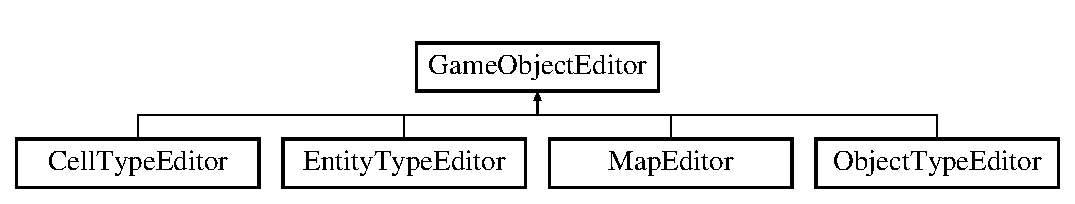
\includegraphics[height=2.000000cm]{class_game_object_editor}
\end{center}
\end{figure}
\subsection*{\-Public \-Member \-Functions}
\begin{DoxyCompactItemize}
\item 
\hypertarget{class_game_object_editor_a3ca8c1b7d22f2f3f8c6b518dae3e21a1}{{\bfseries \-Game\-Object\-Editor} (\-Q\-Widget $\ast$parent=0)}\label{class_game_object_editor_a3ca8c1b7d22f2f3f8c6b518dae3e21a1}

\end{DoxyCompactItemize}
\subsection*{\-Static \-Public \-Member \-Functions}
\begin{DoxyCompactItemize}
\item 
\hypertarget{class_game_object_editor_ad43ed39df888f6b06f9078ab8eff3380}{static \hyperlink{class_game_object_editor}{\-Game\-Object\-Editor} $\ast$ {\bfseries editor} (\hyperlink{class_game_object}{\-Game\-Object} \&obj, \-Q\-Widget $\ast$parent=0)}\label{class_game_object_editor_ad43ed39df888f6b06f9078ab8eff3380}

\end{DoxyCompactItemize}


\-The documentation for this class was generated from the following files\-:\begin{DoxyCompactItemize}
\item 
src/editor/\-G\-U\-I/\-Tabs/\-Object\-Editors/gameobjecteditor.\-h\item 
src/editor/\-G\-U\-I/\-Tabs/\-Object\-Editors/gameobjecteditor.\-cpp\end{DoxyCompactItemize}

\hypertarget{class_game_object_type}{\section{\-Game\-Object\-Type \-Class \-Reference}
\label{class_game_object_type}\index{\-Game\-Object\-Type@{\-Game\-Object\-Type}}
}
\-Inheritance diagram for \-Game\-Object\-Type\-:\begin{figure}[H]
\begin{center}
\leavevmode
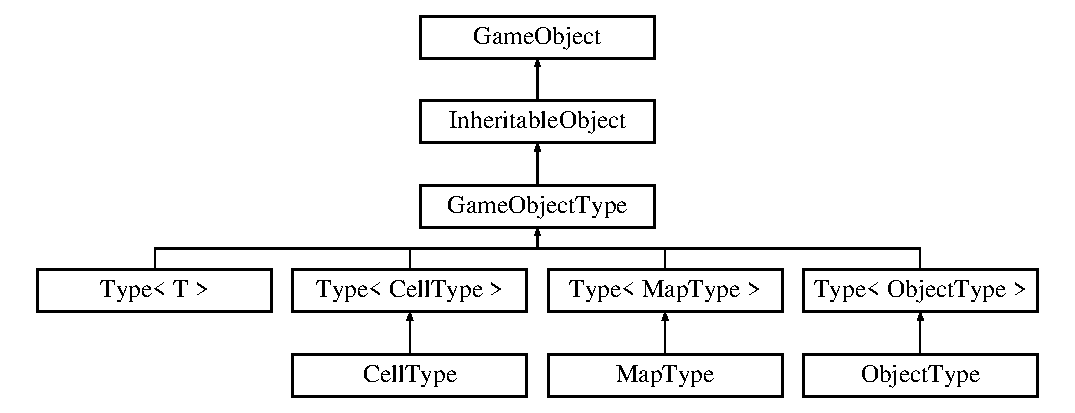
\includegraphics[height=5.000000cm]{class_game_object_type}
\end{center}
\end{figure}
\subsection*{\-Public \-Member \-Functions}
\begin{DoxyCompactItemize}
\item 
const \-Q\-List$<$ \hyperlink{class_game_object_type}{\-Game\-Object\-Type} $\ast$ $>$ \hyperlink{class_game_object_type_a68c3d9aeec4b7b259b03b98aca307397}{descendants} () const 
\end{DoxyCompactItemize}
\subsection*{\-Protected \-Member \-Functions}
\begin{DoxyCompactItemize}
\item 
\hypertarget{class_game_object_type_a7c2ad7a00f9240d2bf29db0ac3b1314f}{{\bfseries \-Game\-Object\-Type} (\hyperlink{class_default_types}{\-Default\-Types} \&\hyperlink{class_game_object_af3deaf39cde23c189765634e32e95bb4}{parent})}\label{class_game_object_type_a7c2ad7a00f9240d2bf29db0ac3b1314f}

\item 
\hypertarget{class_game_object_type_a9388a78893199c74f16edb92ae087dd2}{{\bfseries \-Game\-Object\-Type} (\hyperlink{class_game_object_type}{\-Game\-Object\-Type} \&\hyperlink{class_inheritable_object_ac87a3c55ca4be252c527a29fe162bb15}{ancestor})}\label{class_game_object_type_a9388a78893199c74f16edb92ae087dd2}

\end{DoxyCompactItemize}


\subsection{\-Member \-Function \-Documentation}
\hypertarget{class_game_object_type_a68c3d9aeec4b7b259b03b98aca307397}{\index{\-Game\-Object\-Type@{\-Game\-Object\-Type}!descendants@{descendants}}
\index{descendants@{descendants}!GameObjectType@{\-Game\-Object\-Type}}
\subsubsection[{descendants}]{\setlength{\rightskip}{0pt plus 5cm}const \-Q\-List$<$ {\bf \-Game\-Object\-Type} $\ast$ $>$ {\bf \-Game\-Object\-Type\-::descendants} (
\begin{DoxyParamCaption}
{}
\end{DoxyParamCaption}
) const}}\label{class_game_object_type_a68c3d9aeec4b7b259b03b98aca307397}
\-Returns the list of types that inherite from the current instance. 

\-The documentation for this class was generated from the following files\-:\begin{DoxyCompactItemize}
\item 
src/editor/\-Game/\hyperlink{gameobject_8h}{gameobject.\-h}\item 
src/editor/\-Game/gameobject.\-cpp\end{DoxyCompactItemize}

\hypertarget{class_game_tree_item}{\section{\-Game\-Tree\-Item$<$ \-Param\-Item $>$ \-Class \-Template \-Reference}
\label{class_game_tree_item}\index{\-Game\-Tree\-Item$<$ Param\-Item $>$@{\-Game\-Tree\-Item$<$ Param\-Item $>$}}
}


\-The \hyperlink{class_game_tree_item}{\-Game\-Tree\-Item} define a convienent tree item for the \hyperlink{class_param_tree_item_model}{\-Param\-Tree\-Item\-Model} and \hyperlink{class_flag_tree_item_model}{\-Flag\-Tree\-Item\-Model} classes.  




{\ttfamily \#include $<$attrtreeitemmodel.\-h$>$}

\subsection*{\-Public \-Member \-Functions}
\begin{DoxyCompactItemize}
\item 
\hypertarget{class_game_tree_item_ae7b1b4ef2b52d744bf291d93a836f426}{{\bfseries \-Game\-Tree\-Item} (\hyperlink{class_game_object}{\-Game\-Object} \&obj)}\label{class_game_tree_item_ae7b1b4ef2b52d744bf291d93a836f426}

\item 
\hypertarget{class_game_tree_item_ac5b9c6cdd781269439d9a1855a7e6fe5}{{\bfseries \-Game\-Tree\-Item} (\hyperlink{class_inheritable_object}{\-Inheritable\-Object} \&typ)}\label{class_game_tree_item_ac5b9c6cdd781269439d9a1855a7e6fe5}

\item 
\hypertarget{class_game_tree_item_a036054413680c7849828bda7c5ab797e}{\-Qt\-::\-Item\-Flags {\bfseries flags} (int col) const }\label{class_game_tree_item_a036054413680c7849828bda7c5ab797e}

\item 
\hypertarget{class_game_tree_item_affd0244eba999981e24cca1b078f2a57}{\-Q\-Variant {\bfseries data} (int col, int role) const }\label{class_game_tree_item_affd0244eba999981e24cca1b078f2a57}

\item 
\hypertarget{class_game_tree_item_a37646b54531bf9139a21e2b2b0e6b9d3}{\hyperlink{class_game_tree_item}{\-Game\-Tree\-Item} $\ast$ {\bfseries parent} () const }\label{class_game_tree_item_a37646b54531bf9139a21e2b2b0e6b9d3}

\item 
\hypertarget{class_game_tree_item_a8ee174720560a36f00e134af7a97cf65}{\hyperlink{class_game_tree_item}{\-Game\-Tree\-Item} $\ast$ {\bfseries child} (int row) const }\label{class_game_tree_item_a8ee174720560a36f00e134af7a97cf65}

\item 
\hypertarget{class_game_tree_item_a99f37119fb7c03cccd48919196ae6ef2}{int {\bfseries row\-Count} () const }\label{class_game_tree_item_a99f37119fb7c03cccd48919196ae6ef2}

\item 
\hypertarget{class_game_tree_item_a165fab8ad302d5a08032433c53612014}{int {\bfseries row} () const }\label{class_game_tree_item_a165fab8ad302d5a08032433c53612014}

\item 
\hypertarget{class_game_tree_item_ae0fbc6d3f64882f8593bcfb8e611912b}{bool {\bfseries set\-Data} (int col, \-Q\-Variant value, int role)}\label{class_game_tree_item_ae0fbc6d3f64882f8593bcfb8e611912b}

\item 
\hypertarget{class_game_tree_item_a52f6a8fe1ef6cb41944db7dc33e3c4ef}{void {\bfseries add\-Attr} (const \-Q\-String \&attr)}\label{class_game_tree_item_a52f6a8fe1ef6cb41944db7dc33e3c4ef}

\item 
\hypertarget{class_game_tree_item_ad380cc52e9af8a0b47f62a726bf266c6}{void {\bfseries sort} ()}\label{class_game_tree_item_ad380cc52e9af8a0b47f62a726bf266c6}

\item 
\hypertarget{class_game_tree_item_a803cc4eab83275877eb1ad6a21a8ea8a}{void {\bfseries set\-Attribute\-Row\-Nb} (int r)}\label{class_game_tree_item_a803cc4eab83275877eb1ad6a21a8ea8a}

\end{DoxyCompactItemize}


\subsection{\-Detailed \-Description}
\subsubsection*{template$<$bool \-Param\-Item$>$class Game\-Tree\-Item$<$ Param\-Item $>$}

\-The \hyperlink{class_game_tree_item}{\-Game\-Tree\-Item} define a convienent tree item for the \hyperlink{class_param_tree_item_model}{\-Param\-Tree\-Item\-Model} and \hyperlink{class_flag_tree_item_model}{\-Flag\-Tree\-Item\-Model} classes. 

\-It ensures items to have a parent, and provides abstract item (not related to object, parameter or flag).

\begin{DoxySeeAlso}{\-See also}
\hyperlink{class_param_tree_item_model}{\-Param\-Tree\-Item\-Model}, \hyperlink{class_flag_tree_item_model}{\-Flag\-Tree\-Item\-Model} 
\end{DoxySeeAlso}


\-The documentation for this class was generated from the following files\-:\begin{DoxyCompactItemize}
\item 
src/editor/\-Game/\-Item\-Models/\hyperlink{attrtreeitemmodel_8h}{attrtreeitemmodel.\-h}\item 
src/editor/\-Game/\-Item\-Models/attrtreeitemmodel.\-cpp\end{DoxyCompactItemize}

\hypertarget{class_image}{\section{\-Image \-Class \-Reference}
\label{class_image}\index{\-Image@{\-Image}}
}


\-The \hyperlink{class_image}{\-Image} class stores an external file in a \-Q\-Image, and gives each image ressources a unique identifier.  




{\ttfamily \#include $<$object.\-h$>$}

\-Inheritance diagram for \-Image\-:\begin{figure}[H]
\begin{center}
\leavevmode
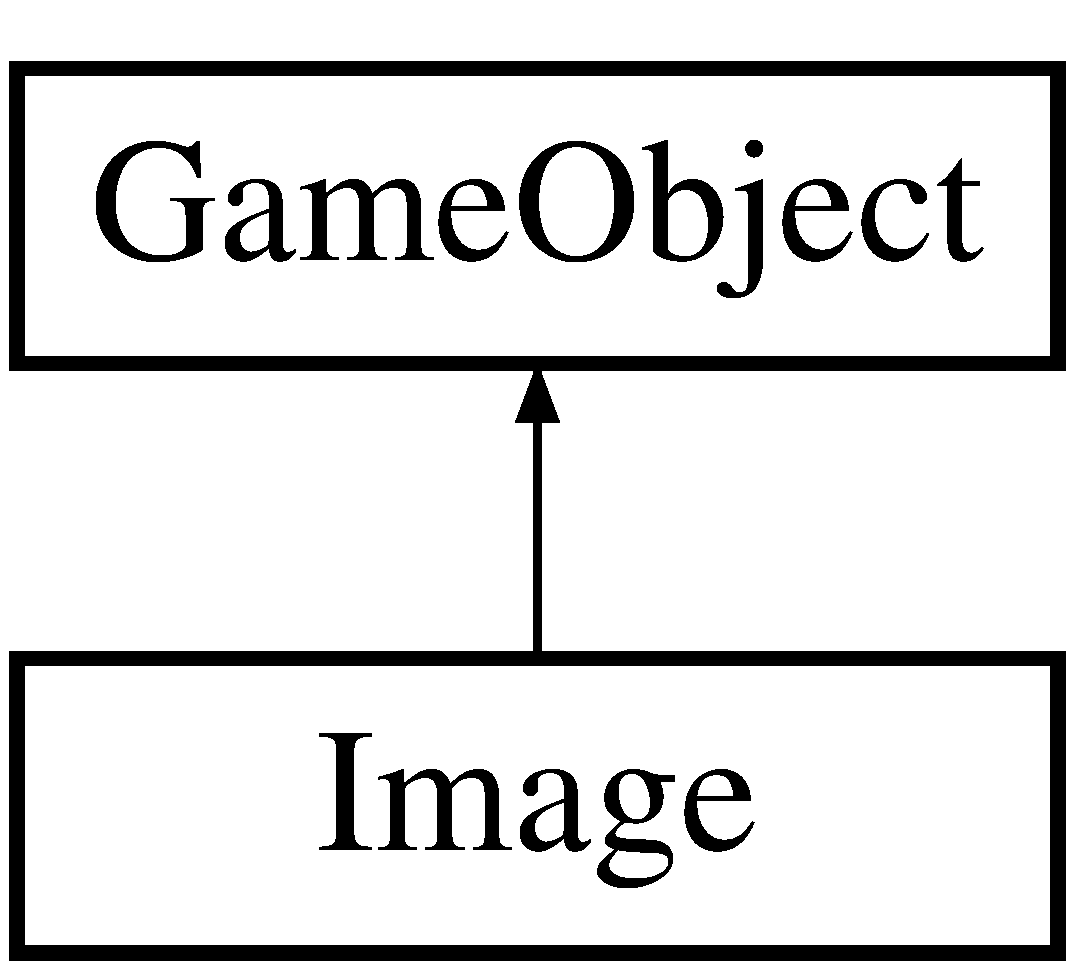
\includegraphics[height=2.000000cm]{class_image}
\end{center}
\end{figure}
\subsection*{\-Public \-Member \-Functions}
\begin{DoxyCompactItemize}
\item 
\hypertarget{class_image_a72923e3d24b0bbf9ff836878ea37091e}{{\bfseries \-Image} (\hyperlink{class_game}{\-Game} $\ast$g, \hyperlink{class_game_object}{\-Game\-Object} $\ast$parent, const \-Q\-String \&file\-Name)}\label{class_image_a72923e3d24b0bbf9ff836878ea37091e}

\item 
bool \hyperlink{class_image_a0bc052fef9ea98e416e11af385cd93b4}{is\-Valid} () const 
\item 
\hypertarget{class_image_abad14459f8cc7bea0ce1b9ce1c41bad1}{const \-Q\-Image \& {\bfseries image} () const }\label{class_image_abad14459f8cc7bea0ce1b9ce1c41bad1}

\item 
\hypertarget{class_image_a62eb0299b2a5109afb31321cba7d4fc8}{const \-Q\-Size {\bfseries size} () const }\label{class_image_a62eb0299b2a5109afb31321cba7d4fc8}

\item 
\hypertarget{class_image_aa4f881e18d7b454ca185c05ec8e70b6d}{void {\bfseries update} ()}\label{class_image_aa4f881e18d7b454ca185c05ec8e70b6d}

\end{DoxyCompactItemize}


\subsection{\-Detailed \-Description}
\-The \hyperlink{class_image}{\-Image} class stores an external file in a \-Q\-Image, and gives each image ressources a unique identifier. 

\subsection{\-Member \-Function \-Documentation}
\hypertarget{class_image_a0bc052fef9ea98e416e11af385cd93b4}{\index{\-Image@{\-Image}!is\-Valid@{is\-Valid}}
\index{is\-Valid@{is\-Valid}!Image@{\-Image}}
\subsubsection[{is\-Valid}]{\setlength{\rightskip}{0pt plus 5cm}bool {\bf \-Image\-::is\-Valid} (
\begin{DoxyParamCaption}
{}
\end{DoxyParamCaption}
) const\hspace{0.3cm}{\ttfamily  \mbox{[}inline, virtual\mbox{]}}}}\label{class_image_a0bc052fef9ea98e416e11af385cd93b4}
\-Returns true if the object has been initialised

\begin{DoxySeeAlso}{\-See also}
\hyperlink{class_game_object_a97be7b59b2e76e7d60de2146b894eed9}{init}, \hyperlink{class_game_object_ab00c537faf6eb4439c60003141a763b9}{\-Game\-Object} 
\end{DoxySeeAlso}


\-Reimplemented from \hyperlink{class_game_object_a88676a10f8e905747f1d64c2da490524}{\-Game\-Object}.



\-The documentation for this class was generated from the following files\-:\begin{DoxyCompactItemize}
\item 
src/editor/\-Game/\hyperlink{object_8h}{object.\-h}\item 
src/editor/\-Game/object.\-cpp\end{DoxyCompactItemize}

\hypertarget{class_inheritable_object}{\section{\-Inheritable\-Object \-Class \-Reference}
\label{class_inheritable_object}\index{\-Inheritable\-Object@{\-Inheritable\-Object}}
}


\-The \hyperlink{class_inheritable_object}{\-Inheritable\-Object} class is the base class for every objects that can inherit attributes from an other \hyperlink{class_inheritable_object}{\-Inheritable\-Object}.  




{\ttfamily \#include $<$gameobject.\-h$>$}

\-Inheritance diagram for \-Inheritable\-Object\-:\begin{figure}[H]
\begin{center}
\leavevmode
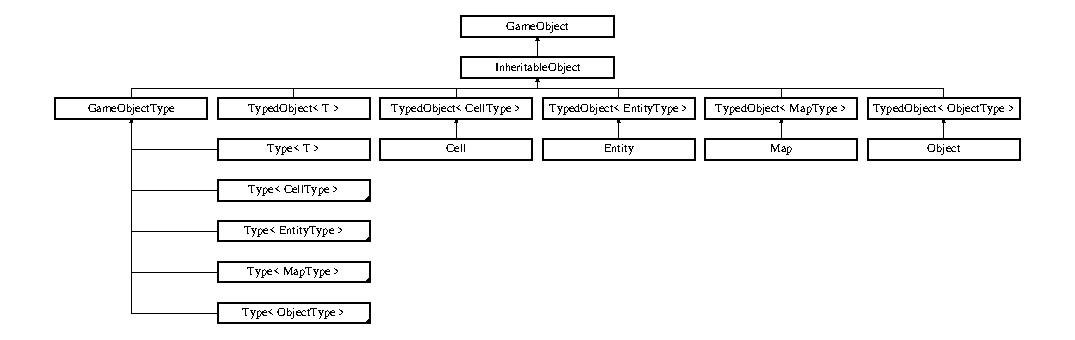
\includegraphics[height=4.125230cm]{class_inheritable_object}
\end{center}
\end{figure}
\subsection*{\-Public \-Member \-Functions}
\begin{DoxyCompactItemize}
\item 
bool \hyperlink{class_inheritable_object_adcbc6cc43d5f999e9c7758f2c15d06da}{has\-Ancestor} () const 
\item 
\hyperlink{class_inheritable_object}{\-Inheritable\-Object} $\ast$ \hyperlink{class_inheritable_object_a10eead70368227b7f15f44f91d234fa5}{ancestor} ()
\item 
virtual bool \hyperlink{class_inheritable_object_a19c749cb2ced87af1b9c0f95920ad60e}{is\-Inherited\-Param} (const \-Q\-String \&param) const 
\item 
virtual bool \hyperlink{class_inheritable_object_abe7d327b43331cd5532c1c8228d63a4e}{is\-Redefinied\-Param} (const \-Q\-String \&param) const 
\item 
virtual int \hyperlink{class_inheritable_object_aa2f45895bcf254ef252428980c06da83}{get\-Param\-Min} (const \-Q\-String \&param) const 
\item 
virtual int \hyperlink{class_inheritable_object_a1edd964a7d01692414ef90f3e88c6a5e}{get\-Param\-Max} (const \-Q\-String \&param) const 
\item 
virtual void \hyperlink{class_inheritable_object_af3ebe709ead7a86ed2eaee602f1ffb67}{set\-Param} (const \-Q\-String \&param, int value)
\item 
virtual int \hyperlink{class_inheritable_object_a85fdb93d54f9e561acf5effa8012abb8}{get\-Param} (const \-Q\-String \&param) const 
\item 
virtual bool \hyperlink{class_inheritable_object_a1f6ee8bcd7cb2e92e260d535518778fc}{has\-Param} (const \-Q\-String \&param) const 
\item 
virtual \-Q\-List$<$ \-Q\-String $>$ \hyperlink{class_inheritable_object_a48233a132cc55bce9f73ca6d2dc7d657}{params} () const 
\item 
virtual \-Q\-List$<$ \-Q\-String $>$ \hyperlink{class_inheritable_object_a6b7782357091c81101b20fb6ca669eb0}{proper\-Params} () const 
\item 
\hyperlink{gameobject_8h_a2679b210263ad72f002dee6909ea222b}{\-Hierarchical\-Attr} \hyperlink{class_inheritable_object_a6bbe68c492529414211ddc8704640d13}{param\-Tree} () const 
\item 
virtual bool \hyperlink{class_inheritable_object_abaae23f6ff5781212a88a5faa4f9ed44}{is\-Inherited\-Flag} (const \-Q\-String \&flag) const 
\item 
virtual bool \hyperlink{class_inheritable_object_ab691081c80168648c19b60061c1fa148}{is\-Redefinied\-Flag} (const \-Q\-String \&flag) const 
\item 
virtual bool \hyperlink{class_inheritable_object_a2982062433ef52c22a669e29dbc42e65}{get\-Flag} (const \-Q\-String \&flag) const 
\item 
virtual bool \hyperlink{class_inheritable_object_a3c441caeca4fdc82fb1978595561f101}{has\-Flag} (const \-Q\-String \&flag) const 
\item 
virtual \-Q\-List$<$ \-Q\-String $>$ \hyperlink{class_inheritable_object_a2014359fb2260eec0804a0e7be0a6c6d}{flags} () const 
\item 
virtual \-Q\-List$<$ \-Q\-String $>$ \hyperlink{class_inheritable_object_a2b0d98c6f8f69698629a4e4c94c85ba4}{proper\-Flags} () const 
\item 
\hyperlink{gameobject_8h_a2679b210263ad72f002dee6909ea222b}{\-Hierarchical\-Attr} \hyperlink{class_inheritable_object_a1f5e307cffd3b9d3fc4c4d00079361f7}{flag\-Tree} () const 
\item 
virtual bool \hyperlink{class_inheritable_object_a8570cbda77efca0b3a8349617f13be3a}{is\-Inherited\-Event} (const \-Q\-String \&event) const 
\item 
virtual bool \hyperlink{class_inheritable_object_a2afb2fbdfad6ecc893038fccbb2d922c}{has\-Event} (const \-Q\-String \&event) const 
\item 
virtual \hyperlink{class_event}{\-Event} \& \hyperlink{class_inheritable_object_abb011de0e529d57bf88160ed6761e0fa}{get\-Event} (const \-Q\-String \&event) const 
\item 
virtual \-Q\-List$<$ \-Q\-String $>$ \hyperlink{class_inheritable_object_af8ff334cb226823e943565509f2f7ac5}{events} () const 
\item 
virtual \-Q\-List$<$ \-Q\-String $>$ \hyperlink{class_inheritable_object_a67a4f5c4e0bf39ffdaf7611e387c1dec}{proper\-Events} () const 
\item 
\hyperlink{gameobject_8h_a2679b210263ad72f002dee6909ea222b}{\-Hierarchical\-Attr} \hyperlink{class_inheritable_object_a5976b3fd18b8ebe7284a61642ab59f5a}{event\-Tree} () const 
\item 
virtual bool \hyperlink{class_inheritable_object_a22092812ca2d4ea9f02baae132204a68}{is\-Inherited\-Order} (const \-Q\-String \&order) const 
\item 
virtual bool \hyperlink{class_inheritable_object_a1c833c8c21936e923364e8f0933c2197}{has\-Order} (const \-Q\-String \&order) const 
\item 
virtual \hyperlink{class_order}{\-Order} \& \hyperlink{class_inheritable_object_a4baa8a0ca7260e9fcda0f9b4d5be4b85}{get\-Order} (const \-Q\-String \&order) const 
\item 
virtual \-Q\-List$<$ \-Q\-String $>$ \hyperlink{class_inheritable_object_a665d17d695bdec5fe43527331bb060f4}{orders} () const 
\item 
virtual \-Q\-List$<$ \-Q\-String $>$ \hyperlink{class_inheritable_object_a775abc07846dcbc608df18fa6ace04cb}{proper\-Orders} () const 
\item 
\hyperlink{gameobject_8h_a2679b210263ad72f002dee6909ea222b}{\-Hierarchical\-Attr} \hyperlink{class_inheritable_object_a63ed35ad744ac4f1e94eccbd82296101}{order\-Tree} () const 
\end{DoxyCompactItemize}
\subsection*{\-Protected \-Member \-Functions}
\begin{DoxyCompactItemize}
\item 
\hypertarget{class_inheritable_object_af01c47efbda743217889d5e0be652c7b}{{\bfseries \-Inheritable\-Object} (\hyperlink{class_game_object}{\-Game\-Object} \&\hyperlink{class_game_object_af3deaf39cde23c189765634e32e95bb4}{parent}, \hyperlink{class_inheritable_object}{\-Inheritable\-Object} $\ast$\hyperlink{class_inheritable_object_a10eead70368227b7f15f44f91d234fa5}{ancestor}=nullptr)}\label{class_inheritable_object_af01c47efbda743217889d5e0be652c7b}

\end{DoxyCompactItemize}
\subsection*{\-Protected \-Attributes}
\begin{DoxyCompactItemize}
\item 
\hypertarget{class_inheritable_object_a985dc4856beac7cd6bbd3a2f534e42ff}{\hyperlink{class_inheritable_object}{\-Inheritable\-Object} $\ast$ {\bfseries a\-Ancestor}}\label{class_inheritable_object_a985dc4856beac7cd6bbd3a2f534e42ff}

\end{DoxyCompactItemize}


\subsection{\-Detailed \-Description}
\-The \hyperlink{class_inheritable_object}{\-Inheritable\-Object} class is the base class for every objects that can inherit attributes from an other \hyperlink{class_inheritable_object}{\-Inheritable\-Object}. 

\begin{DoxyNote}{\-Note}
\-The ancerstor of the object can be modified after instanciation.
\end{DoxyNote}
\-It is the base class of \hyperlink{class_type}{\-Type} and \hyperlink{class_typed_object}{\-Typed\-Object}.

\begin{DoxySeeAlso}{\-See also}
\hyperlink{class_type}{\-Type}, \hyperlink{class_typed_object}{\-Typed\-Object} 
\end{DoxySeeAlso}


\subsection{\-Member \-Function \-Documentation}
\hypertarget{class_inheritable_object_a10eead70368227b7f15f44f91d234fa5}{\index{\-Inheritable\-Object@{\-Inheritable\-Object}!ancestor@{ancestor}}
\index{ancestor@{ancestor}!InheritableObject@{\-Inheritable\-Object}}
\subsubsection[{ancestor}]{\setlength{\rightskip}{0pt plus 5cm}{\bf \-Inheritable\-Object} $\ast$ {\bf \-Inheritable\-Object\-::ancestor} (
\begin{DoxyParamCaption}
{}
\end{DoxyParamCaption}
)}}\label{class_inheritable_object_a10eead70368227b7f15f44f91d234fa5}
\-Returns the object from with the current instance inherits

\begin{DoxySeeAlso}{\-See also}
\hyperlink{class_inheritable_object_adcbc6cc43d5f999e9c7758f2c15d06da}{has\-Ancestor} 
\end{DoxySeeAlso}
\hypertarget{class_inheritable_object_af8ff334cb226823e943565509f2f7ac5}{\index{\-Inheritable\-Object@{\-Inheritable\-Object}!events@{events}}
\index{events@{events}!InheritableObject@{\-Inheritable\-Object}}
\subsubsection[{events}]{\setlength{\rightskip}{0pt plus 5cm}\-Q\-List$<$ \-Q\-String $>$ {\bf \-Inheritable\-Object\-::events} (
\begin{DoxyParamCaption}
{}
\end{DoxyParamCaption}
) const\hspace{0.3cm}{\ttfamily  \mbox{[}virtual\mbox{]}}}}\label{class_inheritable_object_af8ff334cb226823e943565509f2f7ac5}
\-Returns the list of the events of the object, both proper and inherited.

\begin{DoxySeeAlso}{\-See also}
\hyperlink{class_inheritable_object_a67a4f5c4e0bf39ffdaf7611e387c1dec}{proper\-Events}, \hyperlink{class_inheritable_object_a5976b3fd18b8ebe7284a61642ab59f5a}{event\-Tree}, \hyperlink{class_inheritable_object_a48233a132cc55bce9f73ca6d2dc7d657}{params}, \hyperlink{class_inheritable_object_a2014359fb2260eec0804a0e7be0a6c6d}{flags}, \hyperlink{class_inheritable_object_a665d17d695bdec5fe43527331bb060f4}{orders} 
\end{DoxySeeAlso}


\-Reimplemented from \hyperlink{class_game_object_a699357a06b42be80e5f6520320d14745}{\-Game\-Object}.

\hypertarget{class_inheritable_object_a5976b3fd18b8ebe7284a61642ab59f5a}{\index{\-Inheritable\-Object@{\-Inheritable\-Object}!event\-Tree@{event\-Tree}}
\index{event\-Tree@{event\-Tree}!InheritableObject@{\-Inheritable\-Object}}
\subsubsection[{event\-Tree}]{\setlength{\rightskip}{0pt plus 5cm}{\bf \-Hierarchical\-Attr} {\bf \-Inheritable\-Object\-::event\-Tree} (
\begin{DoxyParamCaption}
{}
\end{DoxyParamCaption}
) const}}\label{class_inheritable_object_a5976b3fd18b8ebe7284a61642ab59f5a}
\-Returns the hierarchy of event, that is the list of ancestors and which event they define.

\begin{DoxySeeAlso}{\-See also}
\hyperlink{class_inheritable_object_af8ff334cb226823e943565509f2f7ac5}{events}, \hyperlink{class_inheritable_object_a67a4f5c4e0bf39ffdaf7611e387c1dec}{proper\-Events}, \hyperlink{class_inheritable_object_a6bbe68c492529414211ddc8704640d13}{param\-Tree}, \hyperlink{class_inheritable_object_a1f5e307cffd3b9d3fc4c4d00079361f7}{flag\-Tree}, \hyperlink{class_inheritable_object_a63ed35ad744ac4f1e94eccbd82296101}{order\-Tree} 
\end{DoxySeeAlso}
\hypertarget{class_inheritable_object_a2014359fb2260eec0804a0e7be0a6c6d}{\index{\-Inheritable\-Object@{\-Inheritable\-Object}!flags@{flags}}
\index{flags@{flags}!InheritableObject@{\-Inheritable\-Object}}
\subsubsection[{flags}]{\setlength{\rightskip}{0pt plus 5cm}\-Q\-List$<$ \-Q\-String $>$ {\bf \-Inheritable\-Object\-::flags} (
\begin{DoxyParamCaption}
{}
\end{DoxyParamCaption}
) const\hspace{0.3cm}{\ttfamily  \mbox{[}virtual\mbox{]}}}}\label{class_inheritable_object_a2014359fb2260eec0804a0e7be0a6c6d}
\-Returns the list of the flags of the object, both proper and inherited.

\begin{DoxySeeAlso}{\-See also}
\hyperlink{class_inheritable_object_a2b0d98c6f8f69698629a4e4c94c85ba4}{proper\-Flags}, \hyperlink{class_inheritable_object_a1f5e307cffd3b9d3fc4c4d00079361f7}{flag\-Tree}, \hyperlink{class_inheritable_object_a48233a132cc55bce9f73ca6d2dc7d657}{params}, \hyperlink{class_inheritable_object_af8ff334cb226823e943565509f2f7ac5}{events}, \hyperlink{class_inheritable_object_a665d17d695bdec5fe43527331bb060f4}{orders} 
\end{DoxySeeAlso}


\-Reimplemented from \hyperlink{class_game_object_aa4e80649831f355c14f35f0f9374c691}{\-Game\-Object}.

\hypertarget{class_inheritable_object_a1f5e307cffd3b9d3fc4c4d00079361f7}{\index{\-Inheritable\-Object@{\-Inheritable\-Object}!flag\-Tree@{flag\-Tree}}
\index{flag\-Tree@{flag\-Tree}!InheritableObject@{\-Inheritable\-Object}}
\subsubsection[{flag\-Tree}]{\setlength{\rightskip}{0pt plus 5cm}{\bf \-Hierarchical\-Attr} {\bf \-Inheritable\-Object\-::flag\-Tree} (
\begin{DoxyParamCaption}
{}
\end{DoxyParamCaption}
) const}}\label{class_inheritable_object_a1f5e307cffd3b9d3fc4c4d00079361f7}
\-Returns the hierarchy of flags, that is the list of ancestors and which flags they define.

\begin{DoxySeeAlso}{\-See also}
\hyperlink{class_inheritable_object_a2014359fb2260eec0804a0e7be0a6c6d}{flags}, \hyperlink{class_inheritable_object_a2b0d98c6f8f69698629a4e4c94c85ba4}{proper\-Flags}, \hyperlink{class_inheritable_object_a6bbe68c492529414211ddc8704640d13}{param\-Tree}, \hyperlink{class_inheritable_object_a5976b3fd18b8ebe7284a61642ab59f5a}{event\-Tree}, \hyperlink{class_inheritable_object_a63ed35ad744ac4f1e94eccbd82296101}{order\-Tree} 
\end{DoxySeeAlso}
\hypertarget{class_inheritable_object_abb011de0e529d57bf88160ed6761e0fa}{\index{\-Inheritable\-Object@{\-Inheritable\-Object}!get\-Event@{get\-Event}}
\index{get\-Event@{get\-Event}!InheritableObject@{\-Inheritable\-Object}}
\subsubsection[{get\-Event}]{\setlength{\rightskip}{0pt plus 5cm}{\bf \-Event} \& {\bf \-Inheritable\-Object\-::get\-Event} (
\begin{DoxyParamCaption}
\item[{const \-Q\-String \&}]{event}
\end{DoxyParamCaption}
) const\hspace{0.3cm}{\ttfamily  \mbox{[}virtual\mbox{]}}}}\label{class_inheritable_object_abb011de0e529d57bf88160ed6761e0fa}
\-Returns the {\ttfamily event} event, loocking for it in the different ancestors if not found.

\begin{DoxySeeAlso}{\-See also}
\hyperlink{class_inheritable_object_a2afb2fbdfad6ecc893038fccbb2d922c}{has\-Event}, \hyperlink{class_game_object_a1c078d9c696beb125a3023434cf40053}{\-Game\-Object\-::get\-Event}, \hyperlink{class_inheritable_object_a85fdb93d54f9e561acf5effa8012abb8}{get\-Param}, \hyperlink{class_inheritable_object_a2982062433ef52c22a669e29dbc42e65}{get\-Flag}, \hyperlink{class_inheritable_object_a4baa8a0ca7260e9fcda0f9b4d5be4b85}{get\-Order} 
\end{DoxySeeAlso}


\-Reimplemented from \hyperlink{class_game_object_a1c078d9c696beb125a3023434cf40053}{\-Game\-Object}.

\hypertarget{class_inheritable_object_a2982062433ef52c22a669e29dbc42e65}{\index{\-Inheritable\-Object@{\-Inheritable\-Object}!get\-Flag@{get\-Flag}}
\index{get\-Flag@{get\-Flag}!InheritableObject@{\-Inheritable\-Object}}
\subsubsection[{get\-Flag}]{\setlength{\rightskip}{0pt plus 5cm}bool {\bf \-Inheritable\-Object\-::get\-Flag} (
\begin{DoxyParamCaption}
\item[{const \-Q\-String \&}]{flag}
\end{DoxyParamCaption}
) const\hspace{0.3cm}{\ttfamily  \mbox{[}virtual\mbox{]}}}}\label{class_inheritable_object_a2982062433ef52c22a669e29dbc42e65}
\-Returns the value of the {\ttfamily flag} flag, loocking for it in the different ancestors if not found.

\begin{DoxySeeAlso}{\-See also}
\hyperlink{class_inheritable_object_a2afb2fbdfad6ecc893038fccbb2d922c}{has\-Event}, \hyperlink{class_game_object_a1c078d9c696beb125a3023434cf40053}{\-Game\-Object\-::get\-Event}, \hyperlink{class_inheritable_object_a85fdb93d54f9e561acf5effa8012abb8}{get\-Param}, \hyperlink{class_inheritable_object_abb011de0e529d57bf88160ed6761e0fa}{get\-Event}, \hyperlink{class_inheritable_object_a4baa8a0ca7260e9fcda0f9b4d5be4b85}{get\-Order} 
\end{DoxySeeAlso}


\-Reimplemented from \hyperlink{class_game_object_ac1df89c8a28a491e1cfd102dcbd044d7}{\-Game\-Object}.

\hypertarget{class_inheritable_object_a4baa8a0ca7260e9fcda0f9b4d5be4b85}{\index{\-Inheritable\-Object@{\-Inheritable\-Object}!get\-Order@{get\-Order}}
\index{get\-Order@{get\-Order}!InheritableObject@{\-Inheritable\-Object}}
\subsubsection[{get\-Order}]{\setlength{\rightskip}{0pt plus 5cm}{\bf \-Order} \& {\bf \-Inheritable\-Object\-::get\-Order} (
\begin{DoxyParamCaption}
\item[{const \-Q\-String \&}]{order}
\end{DoxyParamCaption}
) const\hspace{0.3cm}{\ttfamily  \mbox{[}virtual\mbox{]}}}}\label{class_inheritable_object_a4baa8a0ca7260e9fcda0f9b4d5be4b85}
\-Returns the {\ttfamily order} order, loocking for it in the different ancestors if not found.

\begin{DoxySeeAlso}{\-See also}
\hyperlink{class_inheritable_object_a1c833c8c21936e923364e8f0933c2197}{has\-Order}, \hyperlink{class_game_object_a1c078d9c696beb125a3023434cf40053}{\-Game\-Object\-::get\-Event}, \hyperlink{class_inheritable_object_a85fdb93d54f9e561acf5effa8012abb8}{get\-Param}, \hyperlink{class_inheritable_object_a2982062433ef52c22a669e29dbc42e65}{get\-Flag}, \hyperlink{class_inheritable_object_abb011de0e529d57bf88160ed6761e0fa}{get\-Event} 
\end{DoxySeeAlso}


\-Reimplemented from \hyperlink{class_game_object_a42b1228cdea6a0bbff4cdf8c8ee57db7}{\-Game\-Object}.

\hypertarget{class_inheritable_object_a85fdb93d54f9e561acf5effa8012abb8}{\index{\-Inheritable\-Object@{\-Inheritable\-Object}!get\-Param@{get\-Param}}
\index{get\-Param@{get\-Param}!InheritableObject@{\-Inheritable\-Object}}
\subsubsection[{get\-Param}]{\setlength{\rightskip}{0pt plus 5cm}int {\bf \-Inheritable\-Object\-::get\-Param} (
\begin{DoxyParamCaption}
\item[{const \-Q\-String \&}]{param}
\end{DoxyParamCaption}
) const\hspace{0.3cm}{\ttfamily  \mbox{[}virtual\mbox{]}}}}\label{class_inheritable_object_a85fdb93d54f9e561acf5effa8012abb8}
\-Returns the value of the {\ttfamily param} parameter, loocking for it in the different ancestors if not found.

\begin{DoxySeeAlso}{\-See also}
\hyperlink{class_inheritable_object_a2afb2fbdfad6ecc893038fccbb2d922c}{has\-Event}, \hyperlink{class_game_object_a1c078d9c696beb125a3023434cf40053}{\-Game\-Object\-::get\-Event}, \hyperlink{class_inheritable_object_a2982062433ef52c22a669e29dbc42e65}{get\-Flag}, \hyperlink{class_inheritable_object_abb011de0e529d57bf88160ed6761e0fa}{get\-Event}, \hyperlink{class_inheritable_object_a4baa8a0ca7260e9fcda0f9b4d5be4b85}{get\-Order} 
\end{DoxySeeAlso}


\-Reimplemented from \hyperlink{class_game_object_a4c9a0568afb851340b513207c9745734}{\-Game\-Object}.

\hypertarget{class_inheritable_object_a1edd964a7d01692414ef90f3e88c6a5e}{\index{\-Inheritable\-Object@{\-Inheritable\-Object}!get\-Param\-Max@{get\-Param\-Max}}
\index{get\-Param\-Max@{get\-Param\-Max}!InheritableObject@{\-Inheritable\-Object}}
\subsubsection[{get\-Param\-Max}]{\setlength{\rightskip}{0pt plus 5cm}int {\bf \-Inheritable\-Object\-::get\-Param\-Max} (
\begin{DoxyParamCaption}
\item[{const \-Q\-String \&}]{param}
\end{DoxyParamCaption}
) const\hspace{0.3cm}{\ttfamily  \mbox{[}virtual\mbox{]}}}}\label{class_inheritable_object_a1edd964a7d01692414ef90f3e88c6a5e}
\-Returns the upeer bound of the {\ttfamily param} parameter if it exists (or is inherited).

\begin{DoxyNote}{\-Note}
\-If the {\ttfamily param} param is not defined, a default value is returned (100).
\end{DoxyNote}
\begin{DoxySeeAlso}{\-See also}
\hyperlink{class_inheritable_object_a1edd964a7d01692414ef90f3e88c6a5e}{get\-Param\-Max} 
\end{DoxySeeAlso}


\-Reimplemented from \hyperlink{class_game_object_a714857ae1ea08935b8beb76675db33e8}{\-Game\-Object}.

\hypertarget{class_inheritable_object_aa2f45895bcf254ef252428980c06da83}{\index{\-Inheritable\-Object@{\-Inheritable\-Object}!get\-Param\-Min@{get\-Param\-Min}}
\index{get\-Param\-Min@{get\-Param\-Min}!InheritableObject@{\-Inheritable\-Object}}
\subsubsection[{get\-Param\-Min}]{\setlength{\rightskip}{0pt plus 5cm}int {\bf \-Inheritable\-Object\-::get\-Param\-Min} (
\begin{DoxyParamCaption}
\item[{const \-Q\-String \&}]{param}
\end{DoxyParamCaption}
) const\hspace{0.3cm}{\ttfamily  \mbox{[}virtual\mbox{]}}}}\label{class_inheritable_object_aa2f45895bcf254ef252428980c06da83}
\-Returns the lower bound of the {\ttfamily param} parameter if it exists (or is inherited).

\begin{DoxyNote}{\-Note}
\-If the {\ttfamily param} param is not defined, a default value is returned (0).
\end{DoxyNote}
\begin{DoxySeeAlso}{\-See also}
\hyperlink{class_inheritable_object_a1edd964a7d01692414ef90f3e88c6a5e}{get\-Param\-Max} 
\end{DoxySeeAlso}


\-Reimplemented from \hyperlink{class_game_object_a3a308cc3f1d11d66dd5583fb531035c3}{\-Game\-Object}.

\hypertarget{class_inheritable_object_adcbc6cc43d5f999e9c7758f2c15d06da}{\index{\-Inheritable\-Object@{\-Inheritable\-Object}!has\-Ancestor@{has\-Ancestor}}
\index{has\-Ancestor@{has\-Ancestor}!InheritableObject@{\-Inheritable\-Object}}
\subsubsection[{has\-Ancestor}]{\setlength{\rightskip}{0pt plus 5cm}bool {\bf \-Inheritable\-Object\-::has\-Ancestor} (
\begin{DoxyParamCaption}
{}
\end{DoxyParamCaption}
) const}}\label{class_inheritable_object_adcbc6cc43d5f999e9c7758f2c15d06da}
\-Returns {\ttfamily true} if the object inherits from an other one.

\begin{DoxySeeAlso}{\-See also}
\hyperlink{class_inheritable_object_a10eead70368227b7f15f44f91d234fa5}{ancestor} 
\end{DoxySeeAlso}
\hypertarget{class_inheritable_object_a2afb2fbdfad6ecc893038fccbb2d922c}{\index{\-Inheritable\-Object@{\-Inheritable\-Object}!has\-Event@{has\-Event}}
\index{has\-Event@{has\-Event}!InheritableObject@{\-Inheritable\-Object}}
\subsubsection[{has\-Event}]{\setlength{\rightskip}{0pt plus 5cm}bool {\bf \-Inheritable\-Object\-::has\-Event} (
\begin{DoxyParamCaption}
\item[{const \-Q\-String \&}]{event}
\end{DoxyParamCaption}
) const\hspace{0.3cm}{\ttfamily  \mbox{[}virtual\mbox{]}}}}\label{class_inheritable_object_a2afb2fbdfad6ecc893038fccbb2d922c}
\-Returns true if the {\ttfamily event} event is defined in the object or one of its ancestors.

\begin{DoxySeeAlso}{\-See also}
\hyperlink{class_inheritable_object_abb011de0e529d57bf88160ed6761e0fa}{get\-Event}, \hyperlink{class_game_object_a1bb4b921fe5335ad4513e6edcac64deb}{\-Game\-Object\-::has\-Event}, \hyperlink{class_inheritable_object_a1f6ee8bcd7cb2e92e260d535518778fc}{has\-Param}, \hyperlink{class_inheritable_object_a3c441caeca4fdc82fb1978595561f101}{has\-Flag}, \hyperlink{class_inheritable_object_a1c833c8c21936e923364e8f0933c2197}{has\-Order} 
\end{DoxySeeAlso}


\-Reimplemented from \hyperlink{class_game_object_a1bb4b921fe5335ad4513e6edcac64deb}{\-Game\-Object}.

\hypertarget{class_inheritable_object_a3c441caeca4fdc82fb1978595561f101}{\index{\-Inheritable\-Object@{\-Inheritable\-Object}!has\-Flag@{has\-Flag}}
\index{has\-Flag@{has\-Flag}!InheritableObject@{\-Inheritable\-Object}}
\subsubsection[{has\-Flag}]{\setlength{\rightskip}{0pt plus 5cm}bool {\bf \-Inheritable\-Object\-::has\-Flag} (
\begin{DoxyParamCaption}
\item[{const \-Q\-String \&}]{flag}
\end{DoxyParamCaption}
) const\hspace{0.3cm}{\ttfamily  \mbox{[}virtual\mbox{]}}}}\label{class_inheritable_object_a3c441caeca4fdc82fb1978595561f101}
\-Returns true if the {\ttfamily flag} flag is defined in the object or one of its ancestors.

\begin{DoxySeeAlso}{\-See also}
\hyperlink{class_inheritable_object_a2982062433ef52c22a669e29dbc42e65}{get\-Flag}, \hyperlink{class_game_object_af741fb2fb5e879041c2bd95de4156eb6}{\-Game\-Object\-::has\-Flag}, \hyperlink{class_inheritable_object_a1f6ee8bcd7cb2e92e260d535518778fc}{has\-Param}, \hyperlink{class_inheritable_object_a2afb2fbdfad6ecc893038fccbb2d922c}{has\-Event}, \hyperlink{class_inheritable_object_a1c833c8c21936e923364e8f0933c2197}{has\-Order} 
\end{DoxySeeAlso}


\-Reimplemented from \hyperlink{class_game_object_af741fb2fb5e879041c2bd95de4156eb6}{\-Game\-Object}.

\hypertarget{class_inheritable_object_a1c833c8c21936e923364e8f0933c2197}{\index{\-Inheritable\-Object@{\-Inheritable\-Object}!has\-Order@{has\-Order}}
\index{has\-Order@{has\-Order}!InheritableObject@{\-Inheritable\-Object}}
\subsubsection[{has\-Order}]{\setlength{\rightskip}{0pt plus 5cm}bool {\bf \-Inheritable\-Object\-::has\-Order} (
\begin{DoxyParamCaption}
\item[{const \-Q\-String \&}]{order}
\end{DoxyParamCaption}
) const\hspace{0.3cm}{\ttfamily  \mbox{[}virtual\mbox{]}}}}\label{class_inheritable_object_a1c833c8c21936e923364e8f0933c2197}
\-Returns true if the {\ttfamily order} order is defined in the object or one of its ancestors.

\begin{DoxySeeAlso}{\-See also}
\hyperlink{class_inheritable_object_a4baa8a0ca7260e9fcda0f9b4d5be4b85}{get\-Order}, \hyperlink{class_game_object_a950961df9f6d207ffe3593617df9944e}{\-Game\-Object\-::has\-Order}, \hyperlink{class_inheritable_object_a1f6ee8bcd7cb2e92e260d535518778fc}{has\-Param}, \hyperlink{class_inheritable_object_a3c441caeca4fdc82fb1978595561f101}{has\-Flag}, \hyperlink{class_inheritable_object_a2afb2fbdfad6ecc893038fccbb2d922c}{has\-Event} 
\end{DoxySeeAlso}


\-Reimplemented from \hyperlink{class_game_object_a950961df9f6d207ffe3593617df9944e}{\-Game\-Object}.

\hypertarget{class_inheritable_object_a1f6ee8bcd7cb2e92e260d535518778fc}{\index{\-Inheritable\-Object@{\-Inheritable\-Object}!has\-Param@{has\-Param}}
\index{has\-Param@{has\-Param}!InheritableObject@{\-Inheritable\-Object}}
\subsubsection[{has\-Param}]{\setlength{\rightskip}{0pt plus 5cm}bool {\bf \-Inheritable\-Object\-::has\-Param} (
\begin{DoxyParamCaption}
\item[{const \-Q\-String \&}]{param}
\end{DoxyParamCaption}
) const\hspace{0.3cm}{\ttfamily  \mbox{[}virtual\mbox{]}}}}\label{class_inheritable_object_a1f6ee8bcd7cb2e92e260d535518778fc}
\-Returns true if the {\ttfamily param} parameter is defined in the object or one of its ancestors.

\begin{DoxySeeAlso}{\-See also}
\hyperlink{class_inheritable_object_a85fdb93d54f9e561acf5effa8012abb8}{get\-Param}, \hyperlink{class_game_object_ae5272e52ab14e5d87616a5dcaeb62919}{\-Game\-Object\-::has\-Param}, \hyperlink{class_inheritable_object_a3c441caeca4fdc82fb1978595561f101}{has\-Flag}, \hyperlink{class_inheritable_object_a2afb2fbdfad6ecc893038fccbb2d922c}{has\-Event}, \hyperlink{class_inheritable_object_a1c833c8c21936e923364e8f0933c2197}{has\-Order} 
\end{DoxySeeAlso}


\-Reimplemented from \hyperlink{class_game_object_ae5272e52ab14e5d87616a5dcaeb62919}{\-Game\-Object}.

\hypertarget{class_inheritable_object_a8570cbda77efca0b3a8349617f13be3a}{\index{\-Inheritable\-Object@{\-Inheritable\-Object}!is\-Inherited\-Event@{is\-Inherited\-Event}}
\index{is\-Inherited\-Event@{is\-Inherited\-Event}!InheritableObject@{\-Inheritable\-Object}}
\subsubsection[{is\-Inherited\-Event}]{\setlength{\rightskip}{0pt plus 5cm}bool {\bf \-Inheritable\-Object\-::is\-Inherited\-Event} (
\begin{DoxyParamCaption}
\item[{const \-Q\-String \&}]{event}
\end{DoxyParamCaption}
) const\hspace{0.3cm}{\ttfamily  \mbox{[}virtual\mbox{]}}}}\label{class_inheritable_object_a8570cbda77efca0b3a8349617f13be3a}
\-Returns true if the {\ttfamily event} event is define in one of the ancestors of the object.

\begin{DoxySeeAlso}{\-See also}
\hyperlink{class_inheritable_object_a19c749cb2ced87af1b9c0f95920ad60e}{is\-Inherited\-Param}, \hyperlink{class_inheritable_object_abaae23f6ff5781212a88a5faa4f9ed44}{is\-Inherited\-Flag}, \hyperlink{class_inheritable_object_a22092812ca2d4ea9f02baae132204a68}{is\-Inherited\-Order} 
\end{DoxySeeAlso}
\hypertarget{class_inheritable_object_abaae23f6ff5781212a88a5faa4f9ed44}{\index{\-Inheritable\-Object@{\-Inheritable\-Object}!is\-Inherited\-Flag@{is\-Inherited\-Flag}}
\index{is\-Inherited\-Flag@{is\-Inherited\-Flag}!InheritableObject@{\-Inheritable\-Object}}
\subsubsection[{is\-Inherited\-Flag}]{\setlength{\rightskip}{0pt plus 5cm}bool {\bf \-Inheritable\-Object\-::is\-Inherited\-Flag} (
\begin{DoxyParamCaption}
\item[{const \-Q\-String \&}]{flag}
\end{DoxyParamCaption}
) const\hspace{0.3cm}{\ttfamily  \mbox{[}virtual\mbox{]}}}}\label{class_inheritable_object_abaae23f6ff5781212a88a5faa4f9ed44}
\-Returns true if the {\ttfamily flag} flag is define in one of the ancestors of the object.

\begin{DoxySeeAlso}{\-See also}
\hyperlink{class_inheritable_object_ab691081c80168648c19b60061c1fa148}{is\-Redefinied\-Flag}, \hyperlink{class_inheritable_object_a19c749cb2ced87af1b9c0f95920ad60e}{is\-Inherited\-Param} \hyperlink{class_inheritable_object_a8570cbda77efca0b3a8349617f13be3a}{is\-Inherited\-Event}, \hyperlink{class_inheritable_object_a22092812ca2d4ea9f02baae132204a68}{is\-Inherited\-Order} 
\end{DoxySeeAlso}
\hypertarget{class_inheritable_object_a22092812ca2d4ea9f02baae132204a68}{\index{\-Inheritable\-Object@{\-Inheritable\-Object}!is\-Inherited\-Order@{is\-Inherited\-Order}}
\index{is\-Inherited\-Order@{is\-Inherited\-Order}!InheritableObject@{\-Inheritable\-Object}}
\subsubsection[{is\-Inherited\-Order}]{\setlength{\rightskip}{0pt plus 5cm}bool {\bf \-Inheritable\-Object\-::is\-Inherited\-Order} (
\begin{DoxyParamCaption}
\item[{const \-Q\-String \&}]{order}
\end{DoxyParamCaption}
) const\hspace{0.3cm}{\ttfamily  \mbox{[}virtual\mbox{]}}}}\label{class_inheritable_object_a22092812ca2d4ea9f02baae132204a68}
\-Returns true if the {\ttfamily order} order is define in one of the ancestors of the object.

\begin{DoxySeeAlso}{\-See also}
\hyperlink{class_inheritable_object_a19c749cb2ced87af1b9c0f95920ad60e}{is\-Inherited\-Param}, \hyperlink{class_inheritable_object_abaae23f6ff5781212a88a5faa4f9ed44}{is\-Inherited\-Flag} \hyperlink{class_inheritable_object_a8570cbda77efca0b3a8349617f13be3a}{is\-Inherited\-Event} 
\end{DoxySeeAlso}
\hypertarget{class_inheritable_object_a19c749cb2ced87af1b9c0f95920ad60e}{\index{\-Inheritable\-Object@{\-Inheritable\-Object}!is\-Inherited\-Param@{is\-Inherited\-Param}}
\index{is\-Inherited\-Param@{is\-Inherited\-Param}!InheritableObject@{\-Inheritable\-Object}}
\subsubsection[{is\-Inherited\-Param}]{\setlength{\rightskip}{0pt plus 5cm}bool {\bf \-Inheritable\-Object\-::is\-Inherited\-Param} (
\begin{DoxyParamCaption}
\item[{const \-Q\-String \&}]{param}
\end{DoxyParamCaption}
) const\hspace{0.3cm}{\ttfamily  \mbox{[}virtual\mbox{]}}}}\label{class_inheritable_object_a19c749cb2ced87af1b9c0f95920ad60e}
\-Returns true if the {\ttfamily param} parameter is define in one of the ancestors of the object.

\begin{DoxySeeAlso}{\-See also}
\hyperlink{class_inheritable_object_abe7d327b43331cd5532c1c8228d63a4e}{is\-Redefinied\-Param}, \hyperlink{class_inheritable_object_abaae23f6ff5781212a88a5faa4f9ed44}{is\-Inherited\-Flag} \hyperlink{class_inheritable_object_a8570cbda77efca0b3a8349617f13be3a}{is\-Inherited\-Event}, \hyperlink{class_inheritable_object_a22092812ca2d4ea9f02baae132204a68}{is\-Inherited\-Order} 
\end{DoxySeeAlso}
\hypertarget{class_inheritable_object_ab691081c80168648c19b60061c1fa148}{\index{\-Inheritable\-Object@{\-Inheritable\-Object}!is\-Redefinied\-Flag@{is\-Redefinied\-Flag}}
\index{is\-Redefinied\-Flag@{is\-Redefinied\-Flag}!InheritableObject@{\-Inheritable\-Object}}
\subsubsection[{is\-Redefinied\-Flag}]{\setlength{\rightskip}{0pt plus 5cm}bool {\bf \-Inheritable\-Object\-::is\-Redefinied\-Flag} (
\begin{DoxyParamCaption}
\item[{const \-Q\-String \&}]{flag}
\end{DoxyParamCaption}
) const\hspace{0.3cm}{\ttfamily  \mbox{[}virtual\mbox{]}}}}\label{class_inheritable_object_ab691081c80168648c19b60061c1fa148}
\-Returns true if the {\ttfamily flag} flag is an inherited flag with a object proper value.

\begin{DoxySeeAlso}{\-See also}
\hyperlink{class_inheritable_object_abaae23f6ff5781212a88a5faa4f9ed44}{is\-Inherited\-Flag}, \hyperlink{class_inheritable_object_abe7d327b43331cd5532c1c8228d63a4e}{is\-Redefinied\-Param} 
\end{DoxySeeAlso}
\hypertarget{class_inheritable_object_abe7d327b43331cd5532c1c8228d63a4e}{\index{\-Inheritable\-Object@{\-Inheritable\-Object}!is\-Redefinied\-Param@{is\-Redefinied\-Param}}
\index{is\-Redefinied\-Param@{is\-Redefinied\-Param}!InheritableObject@{\-Inheritable\-Object}}
\subsubsection[{is\-Redefinied\-Param}]{\setlength{\rightskip}{0pt plus 5cm}bool {\bf \-Inheritable\-Object\-::is\-Redefinied\-Param} (
\begin{DoxyParamCaption}
\item[{const \-Q\-String \&}]{param}
\end{DoxyParamCaption}
) const\hspace{0.3cm}{\ttfamily  \mbox{[}virtual\mbox{]}}}}\label{class_inheritable_object_abe7d327b43331cd5532c1c8228d63a4e}
\-Returns true if the {\ttfamily param} parameter is an inherited parameter with a object proper value.

\begin{DoxySeeAlso}{\-See also}
\hyperlink{class_inheritable_object_a19c749cb2ced87af1b9c0f95920ad60e}{is\-Inherited\-Param}, \hyperlink{class_inheritable_object_ab691081c80168648c19b60061c1fa148}{is\-Redefinied\-Flag} 
\end{DoxySeeAlso}
\hypertarget{class_inheritable_object_a665d17d695bdec5fe43527331bb060f4}{\index{\-Inheritable\-Object@{\-Inheritable\-Object}!orders@{orders}}
\index{orders@{orders}!InheritableObject@{\-Inheritable\-Object}}
\subsubsection[{orders}]{\setlength{\rightskip}{0pt plus 5cm}\-Q\-List$<$ \-Q\-String $>$ {\bf \-Inheritable\-Object\-::orders} (
\begin{DoxyParamCaption}
{}
\end{DoxyParamCaption}
) const\hspace{0.3cm}{\ttfamily  \mbox{[}virtual\mbox{]}}}}\label{class_inheritable_object_a665d17d695bdec5fe43527331bb060f4}
\-Returns the list of the orders of the object, both proper and inherited.

\begin{DoxySeeAlso}{\-See also}
\hyperlink{class_inheritable_object_a775abc07846dcbc608df18fa6ace04cb}{proper\-Orders}, \hyperlink{class_inheritable_object_a63ed35ad744ac4f1e94eccbd82296101}{order\-Tree}, \hyperlink{class_inheritable_object_a48233a132cc55bce9f73ca6d2dc7d657}{params}, \hyperlink{class_inheritable_object_a2014359fb2260eec0804a0e7be0a6c6d}{flags}, \hyperlink{class_inheritable_object_af8ff334cb226823e943565509f2f7ac5}{events} 
\end{DoxySeeAlso}


\-Reimplemented from \hyperlink{class_game_object_aa11383114a5352c9215517553deb6878}{\-Game\-Object}.

\hypertarget{class_inheritable_object_a63ed35ad744ac4f1e94eccbd82296101}{\index{\-Inheritable\-Object@{\-Inheritable\-Object}!order\-Tree@{order\-Tree}}
\index{order\-Tree@{order\-Tree}!InheritableObject@{\-Inheritable\-Object}}
\subsubsection[{order\-Tree}]{\setlength{\rightskip}{0pt plus 5cm}{\bf \-Hierarchical\-Attr} {\bf \-Inheritable\-Object\-::order\-Tree} (
\begin{DoxyParamCaption}
{}
\end{DoxyParamCaption}
) const}}\label{class_inheritable_object_a63ed35ad744ac4f1e94eccbd82296101}
\-Returns the hierarchy of orders, that is the list of ancestors and which orders they define.

\begin{DoxySeeAlso}{\-See also}
\hyperlink{class_inheritable_object_a665d17d695bdec5fe43527331bb060f4}{orders}, \hyperlink{class_inheritable_object_a775abc07846dcbc608df18fa6ace04cb}{proper\-Orders}, \hyperlink{class_inheritable_object_a6bbe68c492529414211ddc8704640d13}{param\-Tree}, \hyperlink{class_inheritable_object_a1f5e307cffd3b9d3fc4c4d00079361f7}{flag\-Tree}, \hyperlink{class_inheritable_object_a5976b3fd18b8ebe7284a61642ab59f5a}{event\-Tree} 
\end{DoxySeeAlso}
\hypertarget{class_inheritable_object_a48233a132cc55bce9f73ca6d2dc7d657}{\index{\-Inheritable\-Object@{\-Inheritable\-Object}!params@{params}}
\index{params@{params}!InheritableObject@{\-Inheritable\-Object}}
\subsubsection[{params}]{\setlength{\rightskip}{0pt plus 5cm}\-Q\-List$<$ \-Q\-String $>$ {\bf \-Inheritable\-Object\-::params} (
\begin{DoxyParamCaption}
{}
\end{DoxyParamCaption}
) const\hspace{0.3cm}{\ttfamily  \mbox{[}virtual\mbox{]}}}}\label{class_inheritable_object_a48233a132cc55bce9f73ca6d2dc7d657}
\-Returns the list of the parameters of the object, both proper and inherited.

\begin{DoxySeeAlso}{\-See also}
\hyperlink{class_inheritable_object_a6b7782357091c81101b20fb6ca669eb0}{proper\-Params}, \hyperlink{class_inheritable_object_a6bbe68c492529414211ddc8704640d13}{param\-Tree}, \hyperlink{class_inheritable_object_a2014359fb2260eec0804a0e7be0a6c6d}{flags}, \hyperlink{class_inheritable_object_af8ff334cb226823e943565509f2f7ac5}{events}, \hyperlink{class_inheritable_object_a665d17d695bdec5fe43527331bb060f4}{orders} 
\end{DoxySeeAlso}


\-Reimplemented from \hyperlink{class_game_object_a1ef02d136f04abe43628035486dfc254}{\-Game\-Object}.

\hypertarget{class_inheritable_object_a6bbe68c492529414211ddc8704640d13}{\index{\-Inheritable\-Object@{\-Inheritable\-Object}!param\-Tree@{param\-Tree}}
\index{param\-Tree@{param\-Tree}!InheritableObject@{\-Inheritable\-Object}}
\subsubsection[{param\-Tree}]{\setlength{\rightskip}{0pt plus 5cm}{\bf \-Hierarchical\-Attr} {\bf \-Inheritable\-Object\-::param\-Tree} (
\begin{DoxyParamCaption}
{}
\end{DoxyParamCaption}
) const}}\label{class_inheritable_object_a6bbe68c492529414211ddc8704640d13}
\-Returns the hierarchy of parameters, that is the list of ancestors and which parameters they define.

\begin{DoxySeeAlso}{\-See also}
\hyperlink{class_inheritable_object_a48233a132cc55bce9f73ca6d2dc7d657}{params}, \hyperlink{class_inheritable_object_a6b7782357091c81101b20fb6ca669eb0}{proper\-Params}, \hyperlink{class_inheritable_object_a1f5e307cffd3b9d3fc4c4d00079361f7}{flag\-Tree}, \hyperlink{class_inheritable_object_a5976b3fd18b8ebe7284a61642ab59f5a}{event\-Tree}, \hyperlink{class_inheritable_object_a63ed35ad744ac4f1e94eccbd82296101}{order\-Tree} 
\end{DoxySeeAlso}
\hypertarget{class_inheritable_object_a67a4f5c4e0bf39ffdaf7611e387c1dec}{\index{\-Inheritable\-Object@{\-Inheritable\-Object}!proper\-Events@{proper\-Events}}
\index{proper\-Events@{proper\-Events}!InheritableObject@{\-Inheritable\-Object}}
\subsubsection[{proper\-Events}]{\setlength{\rightskip}{0pt plus 5cm}\-Q\-List$<$ \-Q\-String $>$ {\bf \-Inheritable\-Object\-::proper\-Events} (
\begin{DoxyParamCaption}
{}
\end{DoxyParamCaption}
) const\hspace{0.3cm}{\ttfamily  \mbox{[}virtual\mbox{]}}}}\label{class_inheritable_object_a67a4f5c4e0bf39ffdaf7611e387c1dec}
\-Returns the list of the events that are only defined in the object (the uninherited events)

\begin{DoxySeeAlso}{\-See also}
\hyperlink{class_inheritable_object_af8ff334cb226823e943565509f2f7ac5}{events}, \hyperlink{class_inheritable_object_a5976b3fd18b8ebe7284a61642ab59f5a}{event\-Tree}, \hyperlink{class_inheritable_object_a6b7782357091c81101b20fb6ca669eb0}{proper\-Params}, \hyperlink{class_inheritable_object_a2b0d98c6f8f69698629a4e4c94c85ba4}{proper\-Flags}, \hyperlink{class_inheritable_object_a775abc07846dcbc608df18fa6ace04cb}{proper\-Orders} 
\end{DoxySeeAlso}
\hypertarget{class_inheritable_object_a2b0d98c6f8f69698629a4e4c94c85ba4}{\index{\-Inheritable\-Object@{\-Inheritable\-Object}!proper\-Flags@{proper\-Flags}}
\index{proper\-Flags@{proper\-Flags}!InheritableObject@{\-Inheritable\-Object}}
\subsubsection[{proper\-Flags}]{\setlength{\rightskip}{0pt plus 5cm}\-Q\-List$<$ \-Q\-String $>$ {\bf \-Inheritable\-Object\-::proper\-Flags} (
\begin{DoxyParamCaption}
{}
\end{DoxyParamCaption}
) const\hspace{0.3cm}{\ttfamily  \mbox{[}virtual\mbox{]}}}}\label{class_inheritable_object_a2b0d98c6f8f69698629a4e4c94c85ba4}
\-Returns the list of the flags that are only defined in the object (the uninherited flags)

\begin{DoxySeeAlso}{\-See also}
\hyperlink{class_inheritable_object_a2014359fb2260eec0804a0e7be0a6c6d}{flags}, \hyperlink{class_inheritable_object_a1f5e307cffd3b9d3fc4c4d00079361f7}{flag\-Tree}, \hyperlink{class_inheritable_object_a6b7782357091c81101b20fb6ca669eb0}{proper\-Params}, \hyperlink{class_inheritable_object_a67a4f5c4e0bf39ffdaf7611e387c1dec}{proper\-Events}, \hyperlink{class_inheritable_object_a775abc07846dcbc608df18fa6ace04cb}{proper\-Orders} 
\end{DoxySeeAlso}
\hypertarget{class_inheritable_object_a775abc07846dcbc608df18fa6ace04cb}{\index{\-Inheritable\-Object@{\-Inheritable\-Object}!proper\-Orders@{proper\-Orders}}
\index{proper\-Orders@{proper\-Orders}!InheritableObject@{\-Inheritable\-Object}}
\subsubsection[{proper\-Orders}]{\setlength{\rightskip}{0pt plus 5cm}\-Q\-List$<$ \-Q\-String $>$ {\bf \-Inheritable\-Object\-::proper\-Orders} (
\begin{DoxyParamCaption}
{}
\end{DoxyParamCaption}
) const\hspace{0.3cm}{\ttfamily  \mbox{[}virtual\mbox{]}}}}\label{class_inheritable_object_a775abc07846dcbc608df18fa6ace04cb}
\-Returns the list of the orders that are only defined in the object (the uninherited orders)

\begin{DoxySeeAlso}{\-See also}
\hyperlink{class_inheritable_object_a665d17d695bdec5fe43527331bb060f4}{orders}, \hyperlink{class_inheritable_object_a63ed35ad744ac4f1e94eccbd82296101}{order\-Tree}, \hyperlink{class_inheritable_object_a6b7782357091c81101b20fb6ca669eb0}{proper\-Params}, \hyperlink{class_inheritable_object_a2b0d98c6f8f69698629a4e4c94c85ba4}{proper\-Flags}, \hyperlink{class_inheritable_object_a67a4f5c4e0bf39ffdaf7611e387c1dec}{proper\-Events} 
\end{DoxySeeAlso}
\hypertarget{class_inheritable_object_a6b7782357091c81101b20fb6ca669eb0}{\index{\-Inheritable\-Object@{\-Inheritable\-Object}!proper\-Params@{proper\-Params}}
\index{proper\-Params@{proper\-Params}!InheritableObject@{\-Inheritable\-Object}}
\subsubsection[{proper\-Params}]{\setlength{\rightskip}{0pt plus 5cm}\-Q\-List$<$ \-Q\-String $>$ {\bf \-Inheritable\-Object\-::proper\-Params} (
\begin{DoxyParamCaption}
{}
\end{DoxyParamCaption}
) const\hspace{0.3cm}{\ttfamily  \mbox{[}virtual\mbox{]}}}}\label{class_inheritable_object_a6b7782357091c81101b20fb6ca669eb0}
\-Returns the list of the parameters that are only defined in the object (the uninherited parameters)

\begin{DoxySeeAlso}{\-See also}
\hyperlink{class_inheritable_object_a48233a132cc55bce9f73ca6d2dc7d657}{params}, \hyperlink{class_inheritable_object_a6bbe68c492529414211ddc8704640d13}{param\-Tree}, \hyperlink{class_inheritable_object_a2b0d98c6f8f69698629a4e4c94c85ba4}{proper\-Flags}, \hyperlink{class_inheritable_object_a67a4f5c4e0bf39ffdaf7611e387c1dec}{proper\-Events}, \hyperlink{class_inheritable_object_a775abc07846dcbc608df18fa6ace04cb}{proper\-Orders} 
\end{DoxySeeAlso}
\hypertarget{class_inheritable_object_af3ebe709ead7a86ed2eaee602f1ffb67}{\index{\-Inheritable\-Object@{\-Inheritable\-Object}!set\-Param@{set\-Param}}
\index{set\-Param@{set\-Param}!InheritableObject@{\-Inheritable\-Object}}
\subsubsection[{set\-Param}]{\setlength{\rightskip}{0pt plus 5cm}void {\bf \-Inheritable\-Object\-::set\-Param} (
\begin{DoxyParamCaption}
\item[{const \-Q\-String \&}]{param, }
\item[{int}]{value}
\end{DoxyParamCaption}
)\hspace{0.3cm}{\ttfamily  \mbox{[}virtual\mbox{]}}}}\label{class_inheritable_object_af3ebe709ead7a86ed2eaee602f1ffb67}
\-Reimplemented function.

\begin{DoxySeeAlso}{\-See also}
\hyperlink{class_game_object_a2cd8c2defab5b5327a65253b2a6773b9}{\-Game\-Object\-::set\-Param} 
\end{DoxySeeAlso}


\-Reimplemented from \hyperlink{class_game_object_a2cd8c2defab5b5327a65253b2a6773b9}{\-Game\-Object}.



\-The documentation for this class was generated from the following files\-:\begin{DoxyCompactItemize}
\item 
src/editor/\-Game/\hyperlink{gameobject_8h}{gameobject.\-h}\item 
src/editor/\-Game/gameobject.\-cpp\end{DoxyCompactItemize}

\hypertarget{class_intertie}{\section{\-Intertie \-Class \-Reference}
\label{class_intertie}\index{\-Intertie@{\-Intertie}}
}


\-The \hyperlink{class_intertie}{\-Intertie} class provide int that move smoothly from their value to an objective.  




{\ttfamily \#include $<$intertie.\-h$>$}

\subsection*{\-Public \-Slots}
\begin{DoxyCompactItemize}
\item 
\hypertarget{class_intertie_adc4c0f1797d74c01cbe0fed9bc2763ec}{void {\bfseries set\-Value} (int v, bool inert=true)}\label{class_intertie_adc4c0f1797d74c01cbe0fed9bc2763ec}

\item 
\hypertarget{class_intertie_abfd23bc0f2d764bd58997c578c2fad79}{void {\bfseries set\-Maximum\-Speed} (int v\-M)}\label{class_intertie_abfd23bc0f2d764bd58997c578c2fad79}

\item 
\hypertarget{class_intertie_a8911421634e9ec99cf762060f68b8d5e}{void {\bfseries set\-Acceleration} (int a)}\label{class_intertie_a8911421634e9ec99cf762060f68b8d5e}

\item 
\hypertarget{class_intertie_aae62fc52ccd30f0d4606c611a9b5aea8}{void {\bfseries set\-Update\-Interval} (int d)}\label{class_intertie_aae62fc52ccd30f0d4606c611a9b5aea8}

\end{DoxyCompactItemize}
\subsection*{\-Signals}
\begin{DoxyCompactItemize}
\item 
\hypertarget{class_intertie_a6723ac2faa801421b291b9a2b289aedf}{void {\bfseries modification\-Finished} (int)}\label{class_intertie_a6723ac2faa801421b291b9a2b289aedf}

\item 
\hypertarget{class_intertie_ac704099264fb03441f959297513b9f04}{void {\bfseries value\-Changed} (int)}\label{class_intertie_ac704099264fb03441f959297513b9f04}

\end{DoxyCompactItemize}
\subsection*{\-Public \-Member \-Functions}
\begin{DoxyCompactItemize}
\item 
\hypertarget{class_intertie_a5db7f747092208768bc932a15c69fae9}{{\bfseries \-Intertie} (\-Q\-Object $\ast$parent=0)}\label{class_intertie_a5db7f747092208768bc932a15c69fae9}

\item 
\hypertarget{class_intertie_aa30a54fd7c685f48b7d9d178fe6cda6e}{int {\bfseries value} () const }\label{class_intertie_aa30a54fd7c685f48b7d9d178fe6cda6e}

\item 
\hypertarget{class_intertie_a86e5f0e4e5ef985586ccc7596db29c3b}{void {\bfseries link} (\-Q\-Object $\ast$obj, const char $\ast$prop)}\label{class_intertie_a86e5f0e4e5ef985586ccc7596db29c3b}

\end{DoxyCompactItemize}


\subsection{\-Detailed \-Description}
\-The \hyperlink{class_intertie}{\-Intertie} class provide int that move smoothly from their value to an objective. 

\-The documentation for this class was generated from the following files\-:\begin{DoxyCompactItemize}
\item 
src/editor/\-G\-U\-I/\-Tabs/\-Docks/\hyperlink{intertie_8h}{intertie.\-h}\item 
src/editor/\-G\-U\-I/\-Tabs/\-Docks/intertie.\-cpp\end{DoxyCompactItemize}

\hypertarget{class_item_editor}{\section{\-Item\-Editor \-Class \-Reference}
\label{class_item_editor}\index{\-Item\-Editor@{\-Item\-Editor}}
}


\-The \hyperlink{class_item_editor}{\-Item\-Editor} class gives an editor with a \char`\"{}destroy modification\char`\"{} button.  




{\ttfamily \#include $<$itemdelegates.\-h$>$}

\subsection*{\-Public \-Slots}
\begin{DoxyCompactItemize}
\item 
\hypertarget{class_item_editor_abc8de9a31edf1fa50d486e6e31b2ee78}{void {\bfseries data\-Reseted} ()}\label{class_item_editor_abc8de9a31edf1fa50d486e6e31b2ee78}

\item 
\hypertarget{class_item_editor_add462bed1b1bf732ebe2a1272eea8e4c}{void {\bfseries change\-Data} ()}\label{class_item_editor_add462bed1b1bf732ebe2a1272eea8e4c}

\item 
\hypertarget{class_item_editor_a06a93eb64399ff486cb1372cbc8e566d}{void {\bfseries set\-Resetable} (bool r)}\label{class_item_editor_a06a93eb64399ff486cb1372cbc8e566d}

\end{DoxyCompactItemize}
\subsection*{\-Signals}
\begin{DoxyCompactItemize}
\item 
\hypertarget{class_item_editor_a7a3699c869b93d0a412a01fa116cf9c0}{void {\bfseries data\-Changed} (\-Q\-Widget $\ast$)}\label{class_item_editor_a7a3699c869b93d0a412a01fa116cf9c0}

\item 
\hypertarget{class_item_editor_a8d55b2a3b8df5b90e2bc8f1888ac7e7a}{void {\bfseries data\-Reset} (\-Q\-Widget $\ast$)}\label{class_item_editor_a8d55b2a3b8df5b90e2bc8f1888ac7e7a}

\end{DoxyCompactItemize}
\subsection*{\-Public \-Member \-Functions}
\begin{DoxyCompactItemize}
\item 
\hypertarget{class_item_editor_a9ca5d5d8d4ae77e378d069c57dc18ba5}{{\bfseries \-Item\-Editor} (\-Q\-Widget $\ast$edit, bool redef, \-Q\-Widget $\ast$parent)}\label{class_item_editor_a9ca5d5d8d4ae77e378d069c57dc18ba5}

\item 
\hypertarget{class_item_editor_a71ede1af77c2de8f7d1229ccada47f9a}{void {\bfseries set\-Editor\-Property} (const char $\ast$name, const \-Q\-Variant \&value)}\label{class_item_editor_a71ede1af77c2de8f7d1229ccada47f9a}

\item 
\hypertarget{class_item_editor_a782c5756b983fc5993ad65636d4737c5}{\-Q\-Variant {\bfseries editor\-Property} (const char $\ast$name) const }\label{class_item_editor_a782c5756b983fc5993ad65636d4737c5}

\item 
\hypertarget{class_item_editor_ac1ef2ff64a85a0cf7e03483d4c256ee1}{bool {\bfseries reset\-Requested} () const }\label{class_item_editor_ac1ef2ff64a85a0cf7e03483d4c256ee1}

\item 
\hypertarget{class_item_editor_a59d16e179b2526834559467e752e8db0}{\-Q\-Widget $\ast$ {\bfseries editor} () const }\label{class_item_editor_a59d16e179b2526834559467e752e8db0}

\end{DoxyCompactItemize}


\subsection{\-Detailed \-Description}
\-The \hyperlink{class_item_editor}{\-Item\-Editor} class gives an editor with a \char`\"{}destroy modification\char`\"{} button. 

\-The documentation for this class was generated from the following files\-:\begin{DoxyCompactItemize}
\item 
src/editor/\-G\-U\-I/\-Tabs/\hyperlink{itemdelegates_8h}{itemdelegates.\-h}\item 
src/editor/\-G\-U\-I/\-Tabs/itemdelegates.\-cpp\end{DoxyCompactItemize}

\hypertarget{class_map}{\section{\-Map \-Class \-Reference}
\label{class_map}\index{\-Map@{\-Map}}
}


\-The \hyperlink{class_map}{\-Map} class.  




{\ttfamily \#include $<$map.\-h$>$}

\-Inheritance diagram for \-Map\-:\begin{figure}[H]
\begin{center}
\leavevmode
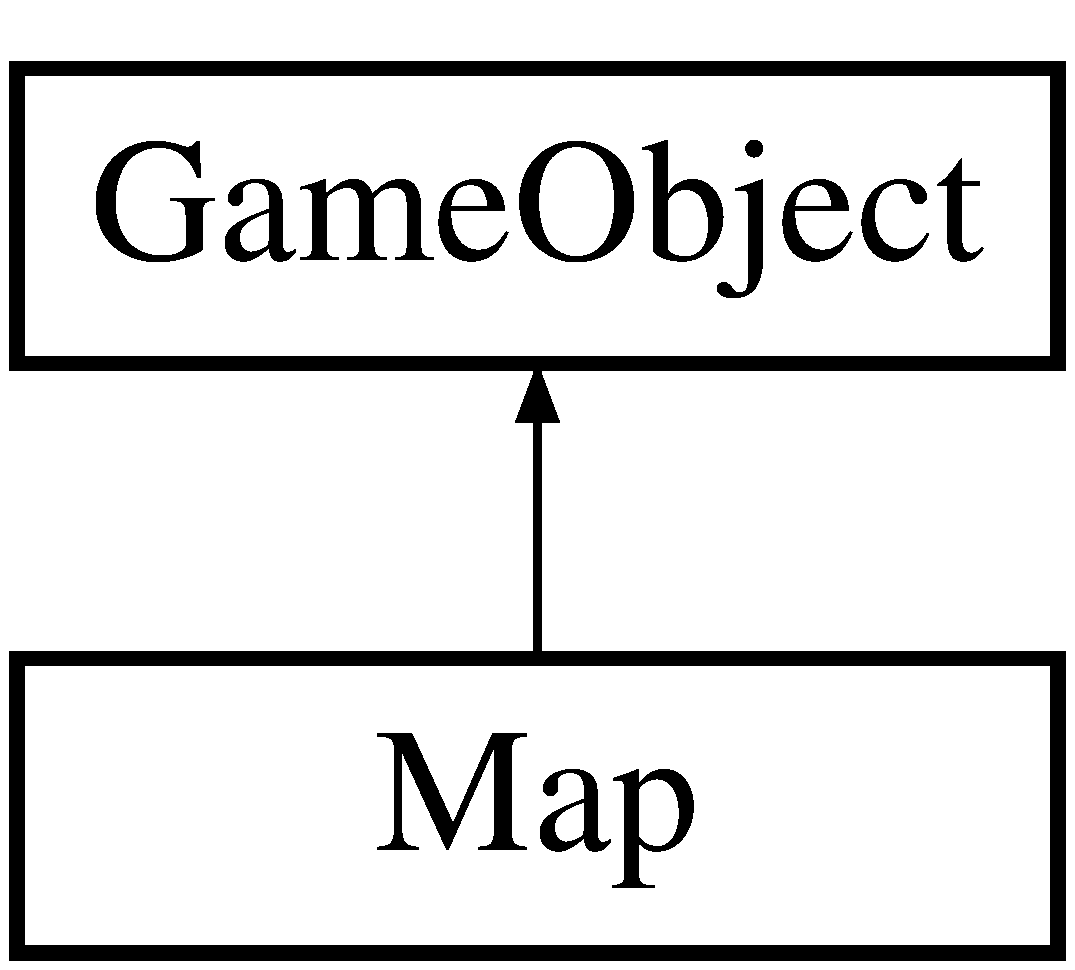
\includegraphics[height=2.000000cm]{class_map}
\end{center}
\end{figure}
\subsection*{\-Public \-Member \-Functions}
\begin{DoxyCompactItemize}
\item 
\hypertarget{class_map_abb18ba5d4ffce18e1813b77b7f6266c9}{{\bfseries \-Type\-Name} (\hyperlink{class_map}{\-Map}) \hyperlink{class_map}{\-Map}(\hyperlink{class_game}{\-Game} $\ast$g}\label{class_map_abb18ba5d4ffce18e1813b77b7f6266c9}

\item 
\hypertarget{class_map_a4c35169a60acd3669f198e6c2d20dff5}{int {\bfseries width} () const }\label{class_map_a4c35169a60acd3669f198e6c2d20dff5}

\item 
\hypertarget{class_map_a009f197c2e488d8dd5f02b1a2920a15c}{int {\bfseries height} () const }\label{class_map_a009f197c2e488d8dd5f02b1a2920a15c}

\item 
\hypertarget{class_map_a028c347d88716e984c943f382f58b7ef}{\-Q\-Size {\bfseries size} () const }\label{class_map_a028c347d88716e984c943f382f58b7ef}

\item 
\hypertarget{class_map_a2915ccde4d8a2ba8142677baea803467}{void {\bfseries set\-Width} (int w)}\label{class_map_a2915ccde4d8a2ba8142677baea803467}

\item 
\hypertarget{class_map_affab3537641a7985559f83ea083e00ca}{void {\bfseries set\-Height} (int h)}\label{class_map_affab3537641a7985559f83ea083e00ca}

\item 
\hypertarget{class_map_a5f7c31af6620d00ce8a812c8710345ab}{void {\bfseries resize} (int w, int h)}\label{class_map_a5f7c31af6620d00ce8a812c8710345ab}

\item 
\hypertarget{class_map_a6c94b3e99490efa0f170db132dc9f5b8}{\hyperlink{class_cell}{\-Cell} \& {\bfseries cell} (int i, int j) const }\label{class_map_a6c94b3e99490efa0f170db132dc9f5b8}

\item 
\hypertarget{class_map_ae0b03b422a10edbfa7bd0b4bdd085793}{\hyperlink{class_cell}{\-Cell} \& {\bfseries cell} (const \-Q\-Point \&p) const }\label{class_map_ae0b03b422a10edbfa7bd0b4bdd085793}

\item 
\hypertarget{class_map_a16aea6b5c9de3a26b094d964885b33b7}{void {\bfseries select\-All} ()}\label{class_map_a16aea6b5c9de3a26b094d964885b33b7}

\item 
\hypertarget{class_map_a5b85190575503a09c5c6de012da64f7c}{void {\bfseries un\-Select\-All} ()}\label{class_map_a5b85190575503a09c5c6de012da64f7c}

\item 
\hypertarget{class_map_a89cab58d82e08dacfe0b97899bab5501}{void {\bfseries confirm\-Pre\-Selection} (bool add=true)}\label{class_map_a89cab58d82e08dacfe0b97899bab5501}

\item 
\hypertarget{class_map_a0a637f44f0a59c3a67b6a507ae710c7f}{void {\bfseries clear\-Pre\-Selection} ()}\label{class_map_a0a637f44f0a59c3a67b6a507ae710c7f}

\item 
\-Q\-List$<$ \hyperlink{class_game_object}{\-Game\-Object} $\ast$ $>$ \hyperlink{class_map_a939817aa7f5c9e81d3d2b1a42d9403e7}{children} () const 
\end{DoxyCompactItemize}
\subsection*{\-Data \-Fields}
\begin{DoxyCompactItemize}
\item 
\hyperlink{class_game_object}{\-Game\-Object} $\ast$ \hyperlink{class_map_ac0d4bf203db2a4372ea6923729f978f1}{a\-Parent}
\end{DoxyCompactItemize}


\subsection{\-Detailed \-Description}
\-The \hyperlink{class_map}{\-Map} class. 

\subsection{\-Member \-Function \-Documentation}
\hypertarget{class_map_a939817aa7f5c9e81d3d2b1a42d9403e7}{\index{\-Map@{\-Map}!children@{children}}
\index{children@{children}!Map@{\-Map}}
\subsubsection[{children}]{\setlength{\rightskip}{0pt plus 5cm}\-Q\-List$<$ {\bf \-Game\-Object} $\ast$ $>$ {\bf \-Map\-::children} (
\begin{DoxyParamCaption}
{}
\end{DoxyParamCaption}
) const\hspace{0.3cm}{\ttfamily  \mbox{[}virtual\mbox{]}}}}\label{class_map_a939817aa7f5c9e81d3d2b1a42d9403e7}
\-Returns the list of the instance's children.

\begin{DoxySeeAlso}{\-See also}
\hyperlink{class_game_object_a6ac392d25a490bee17b653a374ec94fc}{child} 
\end{DoxySeeAlso}


\-Reimplemented from \hyperlink{class_game_object_a3f68b64d3a0793048cfe5deab35397e0}{\-Game\-Object}.



\subsection{\-Field \-Documentation}
\hypertarget{class_map_ac0d4bf203db2a4372ea6923729f978f1}{\index{\-Map@{\-Map}!a\-Parent@{a\-Parent}}
\index{a\-Parent@{a\-Parent}!Map@{\-Map}}
\subsubsection[{a\-Parent}]{\setlength{\rightskip}{0pt plus 5cm}{\bf \-Game\-Object}$\ast$ {\bf \-Map\-::a\-Parent}}}\label{class_map_ac0d4bf203db2a4372ea6923729f978f1}
\-Constructs a new \hyperlink{class_game_object}{\-Game\-Object} with parent {\ttfamily parent} and the reference to the game {\ttfamily g}.

\begin{DoxyNote}{\-Note}
\-If these objects cannot be given to the constructor (case of an array of objects), the \hyperlink{class_game_object_a97be7b59b2e76e7d60de2146b894eed9}{init} method must be called after the creation to make the \hyperlink{class_game_object}{\-Game\-Object} valid. 
\end{DoxyNote}


\-Reimplemented from \hyperlink{class_game_object_a41d4afe43f955e78ede0bbd4ad8957f8}{\-Game\-Object}.



\-The documentation for this class was generated from the following files\-:\begin{DoxyCompactItemize}
\item 
src/editor/\-Game/\hyperlink{map_8h}{map.\-h}\item 
src/editor/\-Game/map.\-cpp\end{DoxyCompactItemize}

\hypertarget{class_map_dock}{}\section{Map\+Dock Class Reference}
\label{class_map_dock}\index{Map\+Dock@{Map\+Dock}}
Inheritance diagram for Map\+Dock\+:\begin{figure}[H]
\begin{center}
\leavevmode
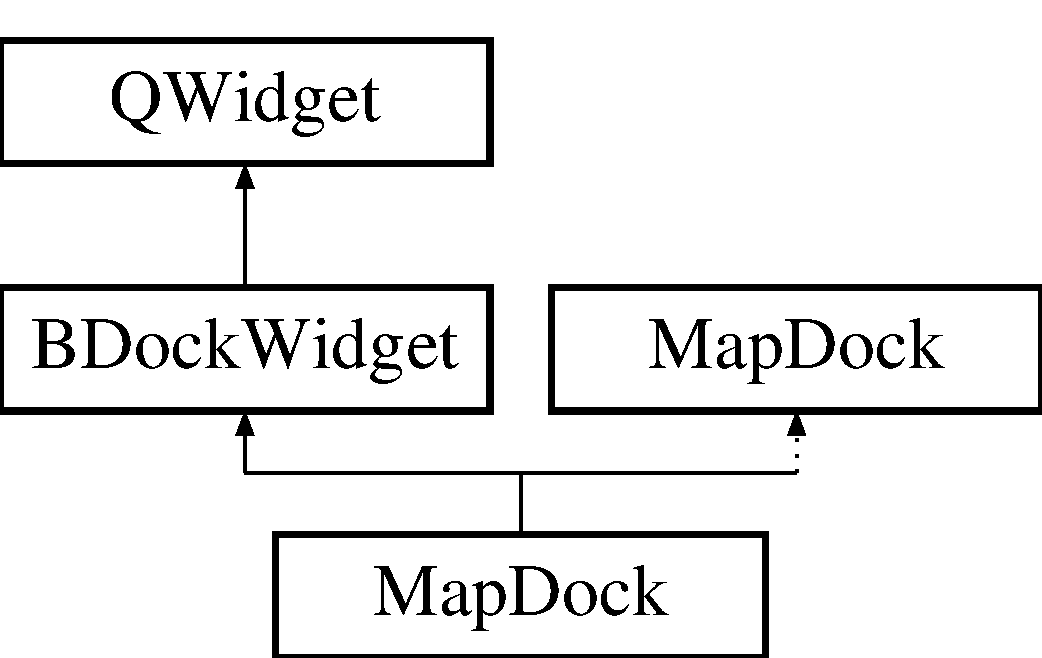
\includegraphics[height=3.000000cm]{class_map_dock}
\end{center}
\end{figure}
\subsection*{Public Member Functions}
\begin{DoxyCompactItemize}
\item 
\hypertarget{class_map_dock_ae65c5f2f8531ec69a9289c8d4731226e}{}\label{class_map_dock_ae65c5f2f8531ec69a9289c8d4731226e} 
{\bfseries Map\+Dock} (Q\+Widget $\ast$parent=0)
\item 
\hypertarget{class_map_dock_a4913eb300e5dd170e9b6c16799731db3}{}\label{class_map_dock_a4913eb300e5dd170e9b6c16799731db3} 
void {\bfseries update\+Game} ()
\end{DoxyCompactItemize}
\subsection*{Additional Inherited Members}


The documentation for this class was generated from the following files\+:\begin{DoxyCompactItemize}
\item 
src/editor/\+G\+U\+I/\+Tabs/mapdock.\+h\item 
src/editor/\+G\+U\+I/\+Tabs/mapdock.\+cpp\end{DoxyCompactItemize}

\hypertarget{class_map_editor}{\section{\-Map\-Editor \-Class \-Reference}
\label{class_map_editor}\index{\-Map\-Editor@{\-Map\-Editor}}
}
\-Inheritance diagram for \-Map\-Editor\-:\begin{figure}[H]
\begin{center}
\leavevmode
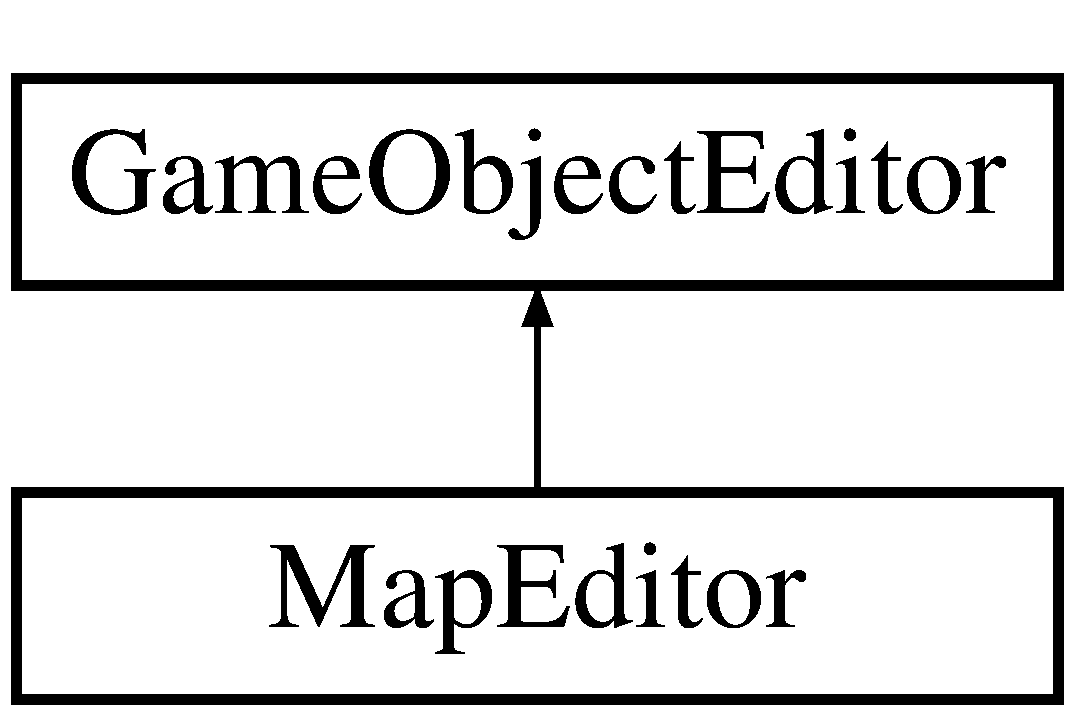
\includegraphics[height=2.000000cm]{class_map_editor}
\end{center}
\end{figure}
\subsection*{\-Signals}
\begin{DoxyCompactItemize}
\item 
\hypertarget{class_map_editor_a6b9ec17c3d4d73b9e7e5a944d81acd9f}{void {\bfseries map\-Modified} ()}\label{class_map_editor_a6b9ec17c3d4d73b9e7e5a944d81acd9f}

\end{DoxyCompactItemize}
\subsection*{\-Public \-Member \-Functions}
\begin{DoxyCompactItemize}
\item 
\hypertarget{class_map_editor_ad30aa4a85a356fef2e41baa6c548a972}{{\bfseries \-Map\-Editor} (\-Q\-Widget $\ast$parent=0)}\label{class_map_editor_ad30aa4a85a356fef2e41baa6c548a972}

\item 
\hypertarget{class_map_editor_a0ee13c368cf79f45e10815e97ffd5c47}{{\bfseries \-Map\-Editor} (\hyperlink{class_map}{\-Map} \&map, \-Q\-Widget $\ast$parent=0)}\label{class_map_editor_a0ee13c368cf79f45e10815e97ffd5c47}

\item 
\hypertarget{class_map_editor_aff674120901fab8e7be3ba92047acdf7}{void {\bfseries set\-Map} (\hyperlink{class_map}{\-Map} \&m)}\label{class_map_editor_aff674120901fab8e7be3ba92047acdf7}

\end{DoxyCompactItemize}


\-The documentation for this class was generated from the following files\-:\begin{DoxyCompactItemize}
\item 
src/editor/\-G\-U\-I/\-Tabs/\-Object\-Editors/mapeditors.\-h\item 
src/editor/\-G\-U\-I/\-Tabs/\-Object\-Editors/mapeditors.\-cpp\end{DoxyCompactItemize}

\hypertarget{class_map_painter}{\section{\-Map\-Painter \-Class \-Reference}
\label{class_map_painter}\index{\-Map\-Painter@{\-Map\-Painter}}
}


\-The \hyperlink{class_map_painter}{\-Map\-Painter} class that can paint a \hyperlink{class_map}{\-Map} using a \-Q\-Painter.  




{\ttfamily \#include $<$mappainter.\-h$>$}

\subsection*{\-Public \-Types}
\begin{DoxyCompactItemize}
\item 
enum \hyperlink{class_map_painter_a771b3fa246b6c13cc2acbdcf1cb6eee3}{\-Element} \{ \*
\hyperlink{class_map_painter_a771b3fa246b6c13cc2acbdcf1cb6eee3a3a60732dd05f5a7cfbb3f823ed15a8af}{\-Nothing} =  0, 
\hyperlink{class_map_painter_a771b3fa246b6c13cc2acbdcf1cb6eee3a26b2d5d6e85f1b419545f806e7e5cda2}{\-Cell\-Background} =  1, 
\hyperlink{class_map_painter_a771b3fa246b6c13cc2acbdcf1cb6eee3a2dcffdfb3d5b1bacc2c5c88cc3642b6a}{\-Grid} =  2, 
\hyperlink{class_map_painter_a771b3fa246b6c13cc2acbdcf1cb6eee3ac4845e6f97ed778c87dec34258ee0290}{\-Cell\-Selection} =  4, 
\*
\hyperlink{class_map_painter_a771b3fa246b6c13cc2acbdcf1cb6eee3a35af0e126a8ff632d0d46c5162ec9a60}{\-Cell\-Highlighting} =  8, 
\hyperlink{class_map_painter_a771b3fa246b6c13cc2acbdcf1cb6eee3a11b1008cd0aafe904943c1a11cb50ad6}{\-Objects} =  16, 
\hyperlink{class_map_painter_a771b3fa246b6c13cc2acbdcf1cb6eee3a25561a3666e5fd539263be7c6e9ab063}{\-All} =  31
 \}
\begin{DoxyCompactList}\small\item\em \-The \-Element enum discribes the different elements that can be render. \end{DoxyCompactList}\end{DoxyCompactItemize}
\subsection*{\-Signals}
\begin{DoxyCompactItemize}
\item 
void \hyperlink{class_map_painter_a8f1f85c58564d01e970bfcaf105e5f9b}{map\-Size\-Changed} (\-Q\-Size)
\item 
void \hyperlink{class_map_painter_a15c872dbb6a7321b978928df5b850ea3}{view\-Center\-Changed} (\-Q\-Point)
\end{DoxyCompactItemize}
\subsection*{\-Public \-Member \-Functions}
\begin{DoxyCompactItemize}
\item 
\hyperlink{class_map_painter_a9c1c9ee90336daa528e090334ef67a39}{\-Map\-Painter} (\-Q\-Object $\ast$parent=0)
\item 
\hyperlink{class_map_painter_a6d282b26150b3d5b592f307f09b29e4c}{\-Map\-Painter} (\hyperlink{class_map}{\-Map} $\ast$m, \-Q\-Object $\ast$parent=0)
\item 
void \hyperlink{class_map_painter_a8e7486d3743d62d2f3d334c23d38e1c9}{set\-Painted\-Element} (\hyperlink{class_map_painter_a771b3fa246b6c13cc2acbdcf1cb6eee3}{\-Element} e, bool painted=true)
\item 
void \hyperlink{class_map_painter_aaf546a511fb08c1688ce06392bce1048}{set\-Painted\-Elements} (\hyperlink{class_map_painter_a771b3fa246b6c13cc2acbdcf1cb6eee3}{\-Element} e)
\item 
void \hyperlink{class_map_painter_a2b1aa596498e0c01c0b53d06d4a598b4}{set\-Map} (\hyperlink{class_map}{\-Map} $\ast$m)
\item 
void \hyperlink{class_map_painter_a0deb552b94eff8f8751946928d7cd5b8}{paint} (\-Q\-Painter \&p)
\item 
const \-Q\-Image \& \hyperlink{class_map_painter_a1c20cf03d0376290481bd80b9f8ef013}{render} ()
\item 
\hyperlink{class_rl_coords}{\-Rl\-Coords} \hyperlink{class_map_painter_acbc0aeb056ee078b0053bf8fb183b36e}{view\-Center} () const 
\item 
void \hyperlink{class_map_painter_a435c535da8087a54ba09c71232377508}{set\-View\-Center} (\hyperlink{class_rl_coords}{\-Rl\-Coords} relative\-Center)
\item 
void \hyperlink{class_map_painter_ae840a2addecd404598ec8300bbd4870f}{set\-View\-Center} (double relative\-Center\-X, double relative\-Center\-Y)
\item 
void \hyperlink{class_map_painter_a5da86b2c104c9d22eb54ecd7b1d0b960}{set\-View\-Center\-Quiet} (double x, double y)
\item 
double \hyperlink{class_map_painter_ae006f2db1575f588b5f94691e9f34970}{scale} () const 
\item 
void \hyperlink{class_map_painter_ae1d7e11835d4ee6588c5b5f0429787e3}{set\-Scale} (double \hyperlink{class_map_painter_ae006f2db1575f588b5f94691e9f34970}{scale})
\item 
void \hyperlink{class_map_painter_afaed21e6944cf1e62398f3f7a0067999}{set\-Scale\-Domain} (double scale\-Min, double scale\-Max)
\item 
bool \hyperlink{class_map_painter_ad7effe1c69fb1409d696dd54edd8bbb3}{set\-Highlighted\-Cell} (const \hyperlink{class_cl_coords}{\-Cl\-Coords} \&p)
\item 
bool \hyperlink{class_map_painter_a49c452342b60a341e7b3530141adeda8}{set\-Highlighted\-Cell} (int i, int j)
\item 
\-Q\-Point \hyperlink{class_map_painter_a528513a51ae87cce652e310587e59f9c}{highlighted\-Cell} () const 
\item 
bool \hyperlink{class_map_painter_ab0f0c512388d95b78d1118af8342fd16}{has\-Highlighted\-Cell} () const 
\item 
bool \hyperlink{class_map_painter_a9d4b59ef444017715bc0d1b4dc1e9d5f}{is\-Cell} (const \hyperlink{class_cl_coords}{\-Cl\-Coords} \&c) const 
\item 
void \hyperlink{class_map_painter_ae215f704c3f1ee11bb89861b9b4b13d3}{resize} (\-Q\-Size s)
\item 
void \hyperlink{class_map_painter_a3280e72c6ffed5e7c550d4632a6de794}{resize} (int wi, int he)
\item 
\-Q\-Size \hyperlink{class_map_painter_a3ae925af3a8a14a83f70b8cbd8c22158}{size} () const 
\item 
void \hyperlink{class_map_painter_a2dacde51513a54fbbf45b44787cd0ee2}{zoom} (double factor, \-Q\-Point\-F fixed\-Point)
\item 
\-Q\-Pair$<$ bool, bool $>$ \hyperlink{class_map_painter_a55dd52865ad3f50b91dadd1f1b6f9352}{move} (\hyperlink{class_px_coords}{\-Px\-Coords} delta, \-Q\-Point\-F center)
\item 
\-Q\-Size \hyperlink{class_map_painter_ac83fce82c6257bd251bc8cd37419af56}{virtual\-Size} () const 
\item 
\hyperlink{class_px_coords}{\-Px\-Coords} \hyperlink{class_map_painter_ac9c2bb380681752eecdd66037ca73192}{pt\-To\-Pxl} (\hyperlink{class_pt_coords}{\-Pt\-Coords} p) const 
\item 
\hyperlink{class_pt_coords}{\-Pt\-Coords} \hyperlink{class_map_painter_af659a9c0dc9d9cd160dafc3aaef9974b}{pxl\-To\-Pt} (\hyperlink{class_px_coords}{\-Px\-Coords} p) const 
\item 
\hyperlink{class_pt_coords}{\-Pt\-Coords} \hyperlink{class_map_painter_a80a2a8fb072ef7e672369a07bb46b059}{coo\-To\-Pt} (\hyperlink{class_cl_coords}{\-Cl\-Coords} p) const 
\item 
\hyperlink{class_cl_coords}{\-Cl\-Coords} \hyperlink{class_map_painter_a00f55d40c322ff5f2038a6515423f9f1}{pt\-To\-Coo} (\hyperlink{class_pt_coords}{\-Pt\-Coords} p) const 
\item 
\hyperlink{class_px_coords}{\-Px\-Coords} \hyperlink{class_map_painter_a4162990e1c9ed17877c0f5a7ad33f606}{coo\-To\-Pxl} (\hyperlink{class_cl_coords}{\-Cl\-Coords} p) const 
\item 
\hyperlink{class_cl_coords}{\-Cl\-Coords} \hyperlink{class_map_painter_a8f14b86f89dabf7183ae960284aaf0b5}{pxl\-To\-Coo} (\hyperlink{class_px_coords}{\-Px\-Coords} p) const 
\item 
\hyperlink{class_pt_coords}{\-Pt\-Coords} \hyperlink{class_map_painter_a1902b1ee672739e47d52a82c4fe3c657}{ind\-To\-Pt} (int i, int j) const 
\item 
const \-Q\-Color \& \hyperlink{class_map_painter_aeb9f8f1f8024a910eb23502189cf911e}{selected\-Cell\-Color} () const 
\item 
const \-Q\-Color \& \hyperlink{class_map_painter_a16c1476ffc1b42de1e3e999ff05f6895}{pre\-Selected\-Cell\-Color} () const 
\item 
void \hyperlink{class_map_painter_ad1658d299eaee7ccdad70f00ad3f76d8}{set\-Selected\-Cell\-Color} (const \-Q\-Color \&c)
\item 
void \hyperlink{class_map_painter_a1c57806b863cd4b83051033681421cf6}{set\-Pre\-Selected\-Cell\-Color} (const \-Q\-Color \&c)
\end{DoxyCompactItemize}


\subsection{\-Detailed \-Description}
\-The \hyperlink{class_map_painter}{\-Map\-Painter} class that can paint a \hyperlink{class_map}{\-Map} using a \-Q\-Painter. 

\-The class take charge of the different ratios of the \hyperlink{class_map}{map} rendering and the area in which it will be rendered.

\begin{DoxyNote}{\-Note}
\-The view is kept updated with the associated \hyperlink{class_map}{map} at each \hyperlink{class_map_painter_a0deb552b94eff8f8751946928d7cd5b8}{paint} or \hyperlink{class_map_painter_a1c20cf03d0376290481bd80b9f8ef013}{render} call. \-It is thus just needed to call one of these functions to update the view after a modification.
\end{DoxyNote}
\-To ensure a type checking security about the different types of coordinates that are used, four different types that inherit from \-Q\-Point\-F are used \-: \hyperlink{class_rl_coords}{\-Rl\-Coords}, \hyperlink{class_cl_coords}{\-Cl\-Coords}, \hyperlink{class_pt_coords}{\-Pt\-Coords} and \hyperlink{class_px_coords}{\-Px\-Coords} 

\subsection{\-Member \-Enumeration \-Documentation}
\hypertarget{class_map_painter_a771b3fa246b6c13cc2acbdcf1cb6eee3}{\index{\-Map\-Painter@{\-Map\-Painter}!\-Element@{\-Element}}
\index{\-Element@{\-Element}!MapPainter@{\-Map\-Painter}}
\subsubsection[{\-Element}]{\setlength{\rightskip}{0pt plus 5cm}enum {\bf \-Map\-Painter\-::\-Element}}}\label{class_map_painter_a771b3fa246b6c13cc2acbdcf1cb6eee3}


\-The \-Element enum discribes the different elements that can be render. 

\-This includes both map's objects and user interaction and editing elements.

\-Element value can be used as flags using the operators operator$|$ \char`\"{}$|$\char`\"{}, operator$|$ \char`\"{}\&\char`\"{}, operator$|$ \char`\"{}$^\wedge$\char`\"{}.

\begin{DoxySeeAlso}{\-See also}
\hyperlink{class_cell}{\-Cell}, \hyperlink{class_cell_type}{\-Cell\-Type} 
\end{DoxySeeAlso}
\begin{Desc}
\item[\-Enumerator\-: ]\par
\begin{description}
\index{\-Nothing@{\-Nothing}!\-Map\-Painter@{\-Map\-Painter}}\index{\-Map\-Painter@{\-Map\-Painter}!\-Nothing@{\-Nothing}}\item[{\em 
\hypertarget{class_map_painter_a771b3fa246b6c13cc2acbdcf1cb6eee3a3a60732dd05f5a7cfbb3f823ed15a8af}{\-Nothing}\label{class_map_painter_a771b3fa246b6c13cc2acbdcf1cb6eee3a3a60732dd05f5a7cfbb3f823ed15a8af}
}]\-Represent no elements \index{\-Cell\-Background@{\-Cell\-Background}!\-Map\-Painter@{\-Map\-Painter}}\index{\-Map\-Painter@{\-Map\-Painter}!\-Cell\-Background@{\-Cell\-Background}}\item[{\em 
\hypertarget{class_map_painter_a771b3fa246b6c13cc2acbdcf1cb6eee3a26b2d5d6e85f1b419545f806e7e5cda2}{\-Cell\-Background}\label{class_map_painter_a771b3fa246b6c13cc2acbdcf1cb6eee3a26b2d5d6e85f1b419545f806e7e5cda2}
}]\-The bacground associated to the \hyperlink{class_cell_type}{cell type} \index{\-Grid@{\-Grid}!\-Map\-Painter@{\-Map\-Painter}}\index{\-Map\-Painter@{\-Map\-Painter}!\-Grid@{\-Grid}}\item[{\em 
\hypertarget{class_map_painter_a771b3fa246b6c13cc2acbdcf1cb6eee3a2dcffdfb3d5b1bacc2c5c88cc3642b6a}{\-Grid}\label{class_map_painter_a771b3fa246b6c13cc2acbdcf1cb6eee3a2dcffdfb3d5b1bacc2c5c88cc3642b6a}
}]\-A thin grid that separate \hyperlink{class_cell}{cells} \index{\-Cell\-Selection@{\-Cell\-Selection}!\-Map\-Painter@{\-Map\-Painter}}\index{\-Map\-Painter@{\-Map\-Painter}!\-Cell\-Selection@{\-Cell\-Selection}}\item[{\em 
\hypertarget{class_map_painter_a771b3fa246b6c13cc2acbdcf1cb6eee3ac4845e6f97ed778c87dec34258ee0290}{\-Cell\-Selection}\label{class_map_painter_a771b3fa246b6c13cc2acbdcf1cb6eee3ac4845e6f97ed778c87dec34258ee0290}
}]\-Graphical information about the selection state \index{\-Cell\-Highlighting@{\-Cell\-Highlighting}!\-Map\-Painter@{\-Map\-Painter}}\index{\-Map\-Painter@{\-Map\-Painter}!\-Cell\-Highlighting@{\-Cell\-Highlighting}}\item[{\em 
\hypertarget{class_map_painter_a771b3fa246b6c13cc2acbdcf1cb6eee3a35af0e126a8ff632d0d46c5162ec9a60}{\-Cell\-Highlighting}\label{class_map_painter_a771b3fa246b6c13cc2acbdcf1cb6eee3a35af0e126a8ff632d0d46c5162ec9a60}
}]\-Graphical visualisation of the \hyperlink{class_cell}{cells} the mouse is over \index{\-Objects@{\-Objects}!\-Map\-Painter@{\-Map\-Painter}}\index{\-Map\-Painter@{\-Map\-Painter}!\-Objects@{\-Objects}}\item[{\em 
\hypertarget{class_map_painter_a771b3fa246b6c13cc2acbdcf1cb6eee3a11b1008cd0aafe904943c1a11cb50ad6}{\-Objects}\label{class_map_painter_a771b3fa246b6c13cc2acbdcf1cb6eee3a11b1008cd0aafe904943c1a11cb50ad6}
}]\-The objects that lay on the \hyperlink{class_cell}{cells} \index{\-All@{\-All}!\-Map\-Painter@{\-Map\-Painter}}\index{\-Map\-Painter@{\-Map\-Painter}!\-All@{\-All}}\item[{\em 
\hypertarget{class_map_painter_a771b3fa246b6c13cc2acbdcf1cb6eee3a25561a3666e5fd539263be7c6e9ab063}{\-All}\label{class_map_painter_a771b3fa246b6c13cc2acbdcf1cb6eee3a25561a3666e5fd539263be7c6e9ab063}
}]\-Represent all elements \end{description}
\end{Desc}



\subsection{\-Constructor \& \-Destructor \-Documentation}
\hypertarget{class_map_painter_a9c1c9ee90336daa528e090334ef67a39}{\index{\-Map\-Painter@{\-Map\-Painter}!\-Map\-Painter@{\-Map\-Painter}}
\index{\-Map\-Painter@{\-Map\-Painter}!MapPainter@{\-Map\-Painter}}
\subsubsection[{\-Map\-Painter}]{\setlength{\rightskip}{0pt plus 5cm}{\bf \-Map\-Painter\-::\-Map\-Painter} (
\begin{DoxyParamCaption}
\item[{\-Q\-Object $\ast$}]{parent = {\ttfamily 0}}
\end{DoxyParamCaption}
)}}\label{class_map_painter_a9c1c9ee90336daa528e090334ef67a39}
\-Constructs a new \hyperlink{class_map_painter}{\-Map\-Painter} with a default size of (42,42). \hypertarget{class_map_painter_a6d282b26150b3d5b592f307f09b29e4c}{\index{\-Map\-Painter@{\-Map\-Painter}!\-Map\-Painter@{\-Map\-Painter}}
\index{\-Map\-Painter@{\-Map\-Painter}!MapPainter@{\-Map\-Painter}}
\subsubsection[{\-Map\-Painter}]{\setlength{\rightskip}{0pt plus 5cm}{\bf \-Map\-Painter\-::\-Map\-Painter} (
\begin{DoxyParamCaption}
\item[{{\bf \-Map} $\ast$}]{m, }
\item[{\-Q\-Object $\ast$}]{parent = {\ttfamily 0}}
\end{DoxyParamCaption}
)}}\label{class_map_painter_a6d282b26150b3d5b592f307f09b29e4c}
\-Constructs a new \hyperlink{class_map_painter}{\-Map\-Painter} with a default size of (42,42), and loads the \hyperlink{class_map}{map} m. 

\subsection{\-Member \-Function \-Documentation}
\hypertarget{class_map_painter_a80a2a8fb072ef7e672369a07bb46b059}{\index{\-Map\-Painter@{\-Map\-Painter}!coo\-To\-Pt@{coo\-To\-Pt}}
\index{coo\-To\-Pt@{coo\-To\-Pt}!MapPainter@{\-Map\-Painter}}
\subsubsection[{coo\-To\-Pt}]{\setlength{\rightskip}{0pt plus 5cm}{\bf \-Pt\-Coords} {\bf \-Map\-Painter\-::coo\-To\-Pt} (
\begin{DoxyParamCaption}
\item[{{\bf \-Cl\-Coords}}]{p}
\end{DoxyParamCaption}
) const}}\label{class_map_painter_a80a2a8fb072ef7e672369a07bb46b059}
\-Converts cells indice to virtual point coordinates \hypertarget{class_map_painter_a4162990e1c9ed17877c0f5a7ad33f606}{\index{\-Map\-Painter@{\-Map\-Painter}!coo\-To\-Pxl@{coo\-To\-Pxl}}
\index{coo\-To\-Pxl@{coo\-To\-Pxl}!MapPainter@{\-Map\-Painter}}
\subsubsection[{coo\-To\-Pxl}]{\setlength{\rightskip}{0pt plus 5cm}{\bf \-Px\-Coords} {\bf \-Map\-Painter\-::coo\-To\-Pxl} (
\begin{DoxyParamCaption}
\item[{{\bf \-Cl\-Coords}}]{p}
\end{DoxyParamCaption}
) const}}\label{class_map_painter_a4162990e1c9ed17877c0f5a7ad33f606}
\-Convenient function equivalent to \hyperlink{class_map_painter_ac9c2bb380681752eecdd66037ca73192}{pt\-To\-Pxl}(\hyperlink{class_map_painter_a80a2a8fb072ef7e672369a07bb46b059}{coo\-To\-Pt}(p)) \hypertarget{class_map_painter_ab0f0c512388d95b78d1118af8342fd16}{\index{\-Map\-Painter@{\-Map\-Painter}!has\-Highlighted\-Cell@{has\-Highlighted\-Cell}}
\index{has\-Highlighted\-Cell@{has\-Highlighted\-Cell}!MapPainter@{\-Map\-Painter}}
\subsubsection[{has\-Highlighted\-Cell}]{\setlength{\rightskip}{0pt plus 5cm}bool {\bf \-Map\-Painter\-::has\-Highlighted\-Cell} (
\begin{DoxyParamCaption}
{}
\end{DoxyParamCaption}
) const}}\label{class_map_painter_ab0f0c512388d95b78d1118af8342fd16}
\-Returns true if a \hyperlink{class_cell}{cell} is highligthed.

\begin{DoxySeeAlso}{\-See also}
\hyperlink{class_map_painter_a528513a51ae87cce652e310587e59f9c}{highlighted\-Cell}, \hyperlink{class_map_painter_ad7effe1c69fb1409d696dd54edd8bbb3}{set\-Highlighted\-Cell} 
\end{DoxySeeAlso}
\hypertarget{class_map_painter_a528513a51ae87cce652e310587e59f9c}{\index{\-Map\-Painter@{\-Map\-Painter}!highlighted\-Cell@{highlighted\-Cell}}
\index{highlighted\-Cell@{highlighted\-Cell}!MapPainter@{\-Map\-Painter}}
\subsubsection[{highlighted\-Cell}]{\setlength{\rightskip}{0pt plus 5cm}\-Q\-Point {\bf \-Map\-Painter\-::highlighted\-Cell} (
\begin{DoxyParamCaption}
{}
\end{DoxyParamCaption}
) const}}\label{class_map_painter_a528513a51ae87cce652e310587e59f9c}
\-Returns the integer index of the \hyperlink{class_cell}{cell} the is highlighted.

\begin{DoxySeeAlso}{\-See also}
\hyperlink{class_map_painter_ad7effe1c69fb1409d696dd54edd8bbb3}{set\-Highlighted\-Cell}, \hyperlink{class_map_painter_ab0f0c512388d95b78d1118af8342fd16}{has\-Highlighted\-Cell} 
\end{DoxySeeAlso}
\hypertarget{class_map_painter_a1902b1ee672739e47d52a82c4fe3c657}{\index{\-Map\-Painter@{\-Map\-Painter}!ind\-To\-Pt@{ind\-To\-Pt}}
\index{ind\-To\-Pt@{ind\-To\-Pt}!MapPainter@{\-Map\-Painter}}
\subsubsection[{ind\-To\-Pt}]{\setlength{\rightskip}{0pt plus 5cm}{\bf \-Pt\-Coords} {\bf \-Map\-Painter\-::ind\-To\-Pt} (
\begin{DoxyParamCaption}
\item[{int}]{i, }
\item[{int}]{j}
\end{DoxyParamCaption}
) const}}\label{class_map_painter_a1902b1ee672739e47d52a82c4fe3c657}
\-Converts to coordinates \hypertarget{class_map_painter_a9d4b59ef444017715bc0d1b4dc1e9d5f}{\index{\-Map\-Painter@{\-Map\-Painter}!is\-Cell@{is\-Cell}}
\index{is\-Cell@{is\-Cell}!MapPainter@{\-Map\-Painter}}
\subsubsection[{is\-Cell}]{\setlength{\rightskip}{0pt plus 5cm}bool {\bf \-Map\-Painter\-::is\-Cell} (
\begin{DoxyParamCaption}
\item[{const {\bf \-Cl\-Coords} \&}]{c}
\end{DoxyParamCaption}
) const}}\label{class_map_painter_a9d4b59ef444017715bc0d1b4dc1e9d5f}
\-Returns true if the coordinate {\ttfamily c} correspond to a \hyperlink{class_cell}{cell}. \hypertarget{class_map_painter_a8f1f85c58564d01e970bfcaf105e5f9b}{\index{\-Map\-Painter@{\-Map\-Painter}!map\-Size\-Changed@{map\-Size\-Changed}}
\index{map\-Size\-Changed@{map\-Size\-Changed}!MapPainter@{\-Map\-Painter}}
\subsubsection[{map\-Size\-Changed}]{\setlength{\rightskip}{0pt plus 5cm}void {\bf \-Map\-Painter\-::map\-Size\-Changed} (
\begin{DoxyParamCaption}
\item[{\-Q\-Size}]{}
\end{DoxyParamCaption}
)\hspace{0.3cm}{\ttfamily  \mbox{[}signal\mbox{]}}}}\label{class_map_painter_a8f1f85c58564d01e970bfcaf105e5f9b}
\-This signal is emitted when the total size of the \hyperlink{class_map}{map}'s view change.

\-It appends mainly during scale change and modification on the \hyperlink{class_map}{map} (resize, angles setting, ...). \hypertarget{class_map_painter_a55dd52865ad3f50b91dadd1f1b6f9352}{\index{\-Map\-Painter@{\-Map\-Painter}!move@{move}}
\index{move@{move}!MapPainter@{\-Map\-Painter}}
\subsubsection[{move}]{\setlength{\rightskip}{0pt plus 5cm}\-Q\-Pair$<$ bool, bool $>$ {\bf \-Map\-Painter\-::move} (
\begin{DoxyParamCaption}
\item[{{\bf \-Px\-Coords}}]{delta, }
\item[{\-Q\-Point\-F}]{center}
\end{DoxyParamCaption}
)}}\label{class_map_painter_a55dd52865ad3f50b91dadd1f1b6f9352}
\-Change the center position from the given center and a pixel difference.

\-The return value indicate if the expected center was valid (regarding x or y coordinate).

\begin{DoxySeeAlso}{\-See also}
\hyperlink{class_map_painter_a435c535da8087a54ba09c71232377508}{set\-View\-Center} 
\end{DoxySeeAlso}
\hypertarget{class_map_painter_a0deb552b94eff8f8751946928d7cd5b8}{\index{\-Map\-Painter@{\-Map\-Painter}!paint@{paint}}
\index{paint@{paint}!MapPainter@{\-Map\-Painter}}
\subsubsection[{paint}]{\setlength{\rightskip}{0pt plus 5cm}void {\bf \-Map\-Painter\-::paint} (
\begin{DoxyParamCaption}
\item[{\-Q\-Painter \&}]{p}
\end{DoxyParamCaption}
)}}\label{class_map_painter_a0deb552b94eff8f8751946928d7cd5b8}
\-Draws the map in the \-Q\-Paint\-Device.

\begin{DoxySeeAlso}{\-See also}
\hyperlink{class_map_painter_a1c20cf03d0376290481bd80b9f8ef013}{render} 
\end{DoxySeeAlso}
\hypertarget{class_map_painter_a16c1476ffc1b42de1e3e999ff05f6895}{\index{\-Map\-Painter@{\-Map\-Painter}!pre\-Selected\-Cell\-Color@{pre\-Selected\-Cell\-Color}}
\index{pre\-Selected\-Cell\-Color@{pre\-Selected\-Cell\-Color}!MapPainter@{\-Map\-Painter}}
\subsubsection[{pre\-Selected\-Cell\-Color}]{\setlength{\rightskip}{0pt plus 5cm}const \-Q\-Color \& {\bf \-Map\-Painter\-::pre\-Selected\-Cell\-Color} (
\begin{DoxyParamCaption}
{}
\end{DoxyParamCaption}
) const}}\label{class_map_painter_a16c1476ffc1b42de1e3e999ff05f6895}
\-Returns the color of the filter that is applied to pre-\/selected cells.

\begin{DoxySeeAlso}{\-See also}
\hyperlink{class_map_painter_a1c57806b863cd4b83051033681421cf6}{set\-Pre\-Selected\-Cell\-Color}, \hyperlink{class_map_painter_aeb9f8f1f8024a910eb23502189cf911e}{selected\-Cell\-Color} 
\end{DoxySeeAlso}
\hypertarget{class_map_painter_a00f55d40c322ff5f2038a6515423f9f1}{\index{\-Map\-Painter@{\-Map\-Painter}!pt\-To\-Coo@{pt\-To\-Coo}}
\index{pt\-To\-Coo@{pt\-To\-Coo}!MapPainter@{\-Map\-Painter}}
\subsubsection[{pt\-To\-Coo}]{\setlength{\rightskip}{0pt plus 5cm}{\bf \-Cl\-Coords} {\bf \-Map\-Painter\-::pt\-To\-Coo} (
\begin{DoxyParamCaption}
\item[{{\bf \-Pt\-Coords}}]{p}
\end{DoxyParamCaption}
) const}}\label{class_map_painter_a00f55d40c322ff5f2038a6515423f9f1}
\-Converts virtual point to cell indice \hypertarget{class_map_painter_ac9c2bb380681752eecdd66037ca73192}{\index{\-Map\-Painter@{\-Map\-Painter}!pt\-To\-Pxl@{pt\-To\-Pxl}}
\index{pt\-To\-Pxl@{pt\-To\-Pxl}!MapPainter@{\-Map\-Painter}}
\subsubsection[{pt\-To\-Pxl}]{\setlength{\rightskip}{0pt plus 5cm}{\bf \-Px\-Coords} {\bf \-Map\-Painter\-::pt\-To\-Pxl} (
\begin{DoxyParamCaption}
\item[{{\bf \-Pt\-Coords}}]{p}
\end{DoxyParamCaption}
) const}}\label{class_map_painter_ac9c2bb380681752eecdd66037ca73192}
\-Converts virtual point to real pixel coordinates \hypertarget{class_map_painter_a8f14b86f89dabf7183ae960284aaf0b5}{\index{\-Map\-Painter@{\-Map\-Painter}!pxl\-To\-Coo@{pxl\-To\-Coo}}
\index{pxl\-To\-Coo@{pxl\-To\-Coo}!MapPainter@{\-Map\-Painter}}
\subsubsection[{pxl\-To\-Coo}]{\setlength{\rightskip}{0pt plus 5cm}{\bf \-Cl\-Coords} {\bf \-Map\-Painter\-::pxl\-To\-Coo} (
\begin{DoxyParamCaption}
\item[{{\bf \-Px\-Coords}}]{p}
\end{DoxyParamCaption}
) const}}\label{class_map_painter_a8f14b86f89dabf7183ae960284aaf0b5}
\-Convenient function equivalent to \hyperlink{class_map_painter_a00f55d40c322ff5f2038a6515423f9f1}{pt\-To\-Coo}(\hyperlink{class_map_painter_af659a9c0dc9d9cd160dafc3aaef9974b}{pxl\-To\-Pt}(p)) \hypertarget{class_map_painter_af659a9c0dc9d9cd160dafc3aaef9974b}{\index{\-Map\-Painter@{\-Map\-Painter}!pxl\-To\-Pt@{pxl\-To\-Pt}}
\index{pxl\-To\-Pt@{pxl\-To\-Pt}!MapPainter@{\-Map\-Painter}}
\subsubsection[{pxl\-To\-Pt}]{\setlength{\rightskip}{0pt plus 5cm}{\bf \-Pt\-Coords} {\bf \-Map\-Painter\-::pxl\-To\-Pt} (
\begin{DoxyParamCaption}
\item[{{\bf \-Px\-Coords}}]{p}
\end{DoxyParamCaption}
) const}}\label{class_map_painter_af659a9c0dc9d9cd160dafc3aaef9974b}
\-Converts real pixel to virtual point coordinates \hypertarget{class_map_painter_a1c20cf03d0376290481bd80b9f8ef013}{\index{\-Map\-Painter@{\-Map\-Painter}!render@{render}}
\index{render@{render}!MapPainter@{\-Map\-Painter}}
\subsubsection[{render}]{\setlength{\rightskip}{0pt plus 5cm}const \-Q\-Image \& {\bf \-Map\-Painter\-::render} (
\begin{DoxyParamCaption}
{}
\end{DoxyParamCaption}
)}}\label{class_map_painter_a1c20cf03d0376290481bd80b9f8ef013}
\-Provides a \-Q\-Image with a view of the map.

\begin{DoxySeeAlso}{\-See also}
\hyperlink{class_map_painter_a0deb552b94eff8f8751946928d7cd5b8}{paint} 
\end{DoxySeeAlso}
\hypertarget{class_map_painter_ae215f704c3f1ee11bb89861b9b4b13d3}{\index{\-Map\-Painter@{\-Map\-Painter}!resize@{resize}}
\index{resize@{resize}!MapPainter@{\-Map\-Painter}}
\subsubsection[{resize}]{\setlength{\rightskip}{0pt plus 5cm}void {\bf \-Map\-Painter\-::resize} (
\begin{DoxyParamCaption}
\item[{\-Q\-Size}]{s}
\end{DoxyParamCaption}
)}}\label{class_map_painter_ae215f704c3f1ee11bb89861b9b4b13d3}
\-Change the size of the view, {\itshape  ie \/} the rectangle in which the map will be render.

\begin{DoxySeeAlso}{\-See also}
\hyperlink{class_map_painter_a3ae925af3a8a14a83f70b8cbd8c22158}{size} 
\end{DoxySeeAlso}
\hypertarget{class_map_painter_a3280e72c6ffed5e7c550d4632a6de794}{\index{\-Map\-Painter@{\-Map\-Painter}!resize@{resize}}
\index{resize@{resize}!MapPainter@{\-Map\-Painter}}
\subsubsection[{resize}]{\setlength{\rightskip}{0pt plus 5cm}void {\bf \-Map\-Painter\-::resize} (
\begin{DoxyParamCaption}
\item[{int}]{wi, }
\item[{int}]{he}
\end{DoxyParamCaption}
)}}\label{class_map_painter_a3280e72c6ffed5e7c550d4632a6de794}
\-This is an overload function, see \hyperlink{class_map_painter_ae215f704c3f1ee11bb89861b9b4b13d3}{resize} \hypertarget{class_map_painter_ae006f2db1575f588b5f94691e9f34970}{\index{\-Map\-Painter@{\-Map\-Painter}!scale@{scale}}
\index{scale@{scale}!MapPainter@{\-Map\-Painter}}
\subsubsection[{scale}]{\setlength{\rightskip}{0pt plus 5cm}double {\bf \-Map\-Painter\-::scale} (
\begin{DoxyParamCaption}
{}
\end{DoxyParamCaption}
) const}}\label{class_map_painter_ae006f2db1575f588b5f94691e9f34970}
\-Returns the current scale of the view.

\begin{DoxySeeAlso}{\-See also}
\hyperlink{class_map_painter_ae1d7e11835d4ee6588c5b5f0429787e3}{set\-Scale} 
\end{DoxySeeAlso}
\hypertarget{class_map_painter_aeb9f8f1f8024a910eb23502189cf911e}{\index{\-Map\-Painter@{\-Map\-Painter}!selected\-Cell\-Color@{selected\-Cell\-Color}}
\index{selected\-Cell\-Color@{selected\-Cell\-Color}!MapPainter@{\-Map\-Painter}}
\subsubsection[{selected\-Cell\-Color}]{\setlength{\rightskip}{0pt plus 5cm}const \-Q\-Color \& {\bf \-Map\-Painter\-::selected\-Cell\-Color} (
\begin{DoxyParamCaption}
{}
\end{DoxyParamCaption}
) const}}\label{class_map_painter_aeb9f8f1f8024a910eb23502189cf911e}
\-Returns the color of the filter that is applied to selected cells.

\begin{DoxySeeAlso}{\-See also}
\hyperlink{class_map_painter_ad1658d299eaee7ccdad70f00ad3f76d8}{set\-Selected\-Cell\-Color}, \hyperlink{class_map_painter_a16c1476ffc1b42de1e3e999ff05f6895}{pre\-Selected\-Cell\-Color} 
\end{DoxySeeAlso}
\hypertarget{class_map_painter_ad7effe1c69fb1409d696dd54edd8bbb3}{\index{\-Map\-Painter@{\-Map\-Painter}!set\-Highlighted\-Cell@{set\-Highlighted\-Cell}}
\index{set\-Highlighted\-Cell@{set\-Highlighted\-Cell}!MapPainter@{\-Map\-Painter}}
\subsubsection[{set\-Highlighted\-Cell}]{\setlength{\rightskip}{0pt plus 5cm}bool {\bf \-Map\-Painter\-::set\-Highlighted\-Cell} (
\begin{DoxyParamCaption}
\item[{const {\bf \-Cl\-Coords} \&}]{p}
\end{DoxyParamCaption}
)}}\label{class_map_painter_ad7effe1c69fb1409d696dd54edd8bbb3}
\-Sets the highligthed \hyperlink{class_cell}{cell} to the one at the \hyperlink{class_cl_coords}{\-Cl\-Coords} p

\begin{DoxySeeAlso}{\-See also}
\hyperlink{class_map_painter_a528513a51ae87cce652e310587e59f9c}{highlighted\-Cell}, \hyperlink{class_map_painter_ab0f0c512388d95b78d1118af8342fd16}{has\-Highlighted\-Cell} 
\end{DoxySeeAlso}
\hypertarget{class_map_painter_a49c452342b60a341e7b3530141adeda8}{\index{\-Map\-Painter@{\-Map\-Painter}!set\-Highlighted\-Cell@{set\-Highlighted\-Cell}}
\index{set\-Highlighted\-Cell@{set\-Highlighted\-Cell}!MapPainter@{\-Map\-Painter}}
\subsubsection[{set\-Highlighted\-Cell}]{\setlength{\rightskip}{0pt plus 5cm}bool {\bf \-Map\-Painter\-::set\-Highlighted\-Cell} (
\begin{DoxyParamCaption}
\item[{int}]{i, }
\item[{int}]{j}
\end{DoxyParamCaption}
)}}\label{class_map_painter_a49c452342b60a341e7b3530141adeda8}
\-This is an overload function, see \hyperlink{class_map_painter_a435c535da8087a54ba09c71232377508}{set\-View\-Center}. \hypertarget{class_map_painter_a2b1aa596498e0c01c0b53d06d4a598b4}{\index{\-Map\-Painter@{\-Map\-Painter}!set\-Map@{set\-Map}}
\index{set\-Map@{set\-Map}!MapPainter@{\-Map\-Painter}}
\subsubsection[{set\-Map}]{\setlength{\rightskip}{0pt plus 5cm}void {\bf \-Map\-Painter\-::set\-Map} (
\begin{DoxyParamCaption}
\item[{{\bf \-Map} $\ast$}]{m}
\end{DoxyParamCaption}
)}}\label{class_map_painter_a2b1aa596498e0c01c0b53d06d4a598b4}
\-Loads the \hyperlink{class_map}{map}, computing the new size of the view area. \hypertarget{class_map_painter_a8e7486d3743d62d2f3d334c23d38e1c9}{\index{\-Map\-Painter@{\-Map\-Painter}!set\-Painted\-Element@{set\-Painted\-Element}}
\index{set\-Painted\-Element@{set\-Painted\-Element}!MapPainter@{\-Map\-Painter}}
\subsubsection[{set\-Painted\-Element}]{\setlength{\rightskip}{0pt plus 5cm}void {\bf \-Map\-Painter\-::set\-Painted\-Element} (
\begin{DoxyParamCaption}
\item[{{\bf \-Map\-Painter\-::\-Element}}]{e, }
\item[{bool}]{painted = {\ttfamily true}}
\end{DoxyParamCaption}
)}}\label{class_map_painter_a8e7486d3743d62d2f3d334c23d38e1c9}
\-Enables or disables the render of an \hyperlink{class_map_painter_a771b3fa246b6c13cc2acbdcf1cb6eee3}{element}.

\begin{DoxySeeAlso}{\-See also}
\hyperlink{class_map_painter_aaf546a511fb08c1688ce06392bce1048}{set\-Painted\-Elements} 
\end{DoxySeeAlso}
\hypertarget{class_map_painter_aaf546a511fb08c1688ce06392bce1048}{\index{\-Map\-Painter@{\-Map\-Painter}!set\-Painted\-Elements@{set\-Painted\-Elements}}
\index{set\-Painted\-Elements@{set\-Painted\-Elements}!MapPainter@{\-Map\-Painter}}
\subsubsection[{set\-Painted\-Elements}]{\setlength{\rightskip}{0pt plus 5cm}void {\bf \-Map\-Painter\-::set\-Painted\-Elements} (
\begin{DoxyParamCaption}
\item[{{\bf \-Element}}]{e}
\end{DoxyParamCaption}
)}}\label{class_map_painter_aaf546a511fb08c1688ce06392bce1048}
\-Sets the rendered \hyperlink{class_map_painter_a771b3fa246b6c13cc2acbdcf1cb6eee3}{elements}.

\begin{DoxySeeAlso}{\-See also}
\hyperlink{class_map_painter_a8e7486d3743d62d2f3d334c23d38e1c9}{set\-Painted\-Element} 
\end{DoxySeeAlso}
\hypertarget{class_map_painter_a1c57806b863cd4b83051033681421cf6}{\index{\-Map\-Painter@{\-Map\-Painter}!set\-Pre\-Selected\-Cell\-Color@{set\-Pre\-Selected\-Cell\-Color}}
\index{set\-Pre\-Selected\-Cell\-Color@{set\-Pre\-Selected\-Cell\-Color}!MapPainter@{\-Map\-Painter}}
\subsubsection[{set\-Pre\-Selected\-Cell\-Color}]{\setlength{\rightskip}{0pt plus 5cm}void {\bf \-Map\-Painter\-::set\-Pre\-Selected\-Cell\-Color} (
\begin{DoxyParamCaption}
\item[{const \-Q\-Color \&}]{c}
\end{DoxyParamCaption}
)}}\label{class_map_painter_a1c57806b863cd4b83051033681421cf6}
\-Sets the color of the filter that is applied to pre-\/selected cells.

\begin{DoxySeeAlso}{\-See also}
\hyperlink{class_map_painter_a16c1476ffc1b42de1e3e999ff05f6895}{pre\-Selected\-Cell\-Color}, \hyperlink{class_map_painter_ad1658d299eaee7ccdad70f00ad3f76d8}{set\-Selected\-Cell\-Color} 
\end{DoxySeeAlso}
\hypertarget{class_map_painter_ae1d7e11835d4ee6588c5b5f0429787e3}{\index{\-Map\-Painter@{\-Map\-Painter}!set\-Scale@{set\-Scale}}
\index{set\-Scale@{set\-Scale}!MapPainter@{\-Map\-Painter}}
\subsubsection[{set\-Scale}]{\setlength{\rightskip}{0pt plus 5cm}void {\bf \-Map\-Painter\-::set\-Scale} (
\begin{DoxyParamCaption}
\item[{double}]{scale}
\end{DoxyParamCaption}
)}}\label{class_map_painter_ae1d7e11835d4ee6588c5b5f0429787e3}
\-Sets the current view scale. \-This closest value in the scale domain will be used.

\begin{DoxySeeAlso}{\-See also}
\hyperlink{class_map_painter_ae006f2db1575f588b5f94691e9f34970}{scale}, \hyperlink{class_map_painter_afaed21e6944cf1e62398f3f7a0067999}{set\-Scale\-Domain} 
\end{DoxySeeAlso}
\hypertarget{class_map_painter_afaed21e6944cf1e62398f3f7a0067999}{\index{\-Map\-Painter@{\-Map\-Painter}!set\-Scale\-Domain@{set\-Scale\-Domain}}
\index{set\-Scale\-Domain@{set\-Scale\-Domain}!MapPainter@{\-Map\-Painter}}
\subsubsection[{set\-Scale\-Domain}]{\setlength{\rightskip}{0pt plus 5cm}void {\bf \-Map\-Painter\-::set\-Scale\-Domain} (
\begin{DoxyParamCaption}
\item[{double}]{scale\-Min, }
\item[{double}]{scale\-Max}
\end{DoxyParamCaption}
)}}\label{class_map_painter_afaed21e6944cf1e62398f3f7a0067999}
\-Sets the valid values for the scale.

\begin{DoxySeeAlso}{\-See also}
\hyperlink{class_map_painter_ae006f2db1575f588b5f94691e9f34970}{scale}, \hyperlink{class_map_painter_ae1d7e11835d4ee6588c5b5f0429787e3}{set\-Scale} 
\end{DoxySeeAlso}
\hypertarget{class_map_painter_ad1658d299eaee7ccdad70f00ad3f76d8}{\index{\-Map\-Painter@{\-Map\-Painter}!set\-Selected\-Cell\-Color@{set\-Selected\-Cell\-Color}}
\index{set\-Selected\-Cell\-Color@{set\-Selected\-Cell\-Color}!MapPainter@{\-Map\-Painter}}
\subsubsection[{set\-Selected\-Cell\-Color}]{\setlength{\rightskip}{0pt plus 5cm}void {\bf \-Map\-Painter\-::set\-Selected\-Cell\-Color} (
\begin{DoxyParamCaption}
\item[{const \-Q\-Color \&}]{c}
\end{DoxyParamCaption}
)}}\label{class_map_painter_ad1658d299eaee7ccdad70f00ad3f76d8}
\-Sets the color of the filter that is applied to selected cells.

\begin{DoxySeeAlso}{\-See also}
\hyperlink{class_map_painter_aeb9f8f1f8024a910eb23502189cf911e}{selected\-Cell\-Color}, \hyperlink{class_map_painter_a1c57806b863cd4b83051033681421cf6}{set\-Pre\-Selected\-Cell\-Color} 
\end{DoxySeeAlso}
\hypertarget{class_map_painter_a435c535da8087a54ba09c71232377508}{\index{\-Map\-Painter@{\-Map\-Painter}!set\-View\-Center@{set\-View\-Center}}
\index{set\-View\-Center@{set\-View\-Center}!MapPainter@{\-Map\-Painter}}
\subsubsection[{set\-View\-Center}]{\setlength{\rightskip}{0pt plus 5cm}void {\bf \-Map\-Painter\-::set\-View\-Center} (
\begin{DoxyParamCaption}
\item[{{\bf \-Rl\-Coords}}]{relative\-Center}
\end{DoxyParamCaption}
)}}\label{class_map_painter_a435c535da8087a54ba09c71232377508}
\-Change the view center, using relative coordinates.

\-If the new center is invalid (the view exceed the map area), the closest valid center is used.

\begin{DoxySeeAlso}{\-See also}
\hyperlink{class_map_painter_acbc0aeb056ee078b0053bf8fb183b36e}{view\-Center} 
\end{DoxySeeAlso}
\hypertarget{class_map_painter_ae840a2addecd404598ec8300bbd4870f}{\index{\-Map\-Painter@{\-Map\-Painter}!set\-View\-Center@{set\-View\-Center}}
\index{set\-View\-Center@{set\-View\-Center}!MapPainter@{\-Map\-Painter}}
\subsubsection[{set\-View\-Center}]{\setlength{\rightskip}{0pt plus 5cm}void {\bf \-Map\-Painter\-::set\-View\-Center} (
\begin{DoxyParamCaption}
\item[{double}]{relative\-Center\-X, }
\item[{double}]{relative\-Center\-Y}
\end{DoxyParamCaption}
)}}\label{class_map_painter_ae840a2addecd404598ec8300bbd4870f}
\-This is an overload function, see \hyperlink{class_map_painter_a435c535da8087a54ba09c71232377508}{set\-View\-Center}. \hypertarget{class_map_painter_a5da86b2c104c9d22eb54ecd7b1d0b960}{\index{\-Map\-Painter@{\-Map\-Painter}!set\-View\-Center\-Quiet@{set\-View\-Center\-Quiet}}
\index{set\-View\-Center\-Quiet@{set\-View\-Center\-Quiet}!MapPainter@{\-Map\-Painter}}
\subsubsection[{set\-View\-Center\-Quiet}]{\setlength{\rightskip}{0pt plus 5cm}void {\bf \-Map\-Painter\-::set\-View\-Center\-Quiet} (
\begin{DoxyParamCaption}
\item[{double}]{x, }
\item[{double}]{y}
\end{DoxyParamCaption}
)}}\label{class_map_painter_a5da86b2c104c9d22eb54ecd7b1d0b960}
does the same as \hyperlink{class_map_painter_a435c535da8087a54ba09c71232377508}{set\-View\-Center}, without emitting the signal view\-Center\-Changed to avoid event loop. \hypertarget{class_map_painter_a3ae925af3a8a14a83f70b8cbd8c22158}{\index{\-Map\-Painter@{\-Map\-Painter}!size@{size}}
\index{size@{size}!MapPainter@{\-Map\-Painter}}
\subsubsection[{size}]{\setlength{\rightskip}{0pt plus 5cm}\-Q\-Size {\bf \-Map\-Painter\-::size} (
\begin{DoxyParamCaption}
{}
\end{DoxyParamCaption}
) const}}\label{class_map_painter_a3ae925af3a8a14a83f70b8cbd8c22158}
\-Return the size of the rectangle in which the map is render. \-This is also the size of the image returned by \hyperlink{class_map_painter_a1c20cf03d0376290481bd80b9f8ef013}{render}.

\begin{DoxySeeAlso}{\-See also}
\hyperlink{class_map_painter_ae215f704c3f1ee11bb89861b9b4b13d3}{resize} 
\end{DoxySeeAlso}
\hypertarget{class_map_painter_acbc0aeb056ee078b0053bf8fb183b36e}{\index{\-Map\-Painter@{\-Map\-Painter}!view\-Center@{view\-Center}}
\index{view\-Center@{view\-Center}!MapPainter@{\-Map\-Painter}}
\subsubsection[{view\-Center}]{\setlength{\rightskip}{0pt plus 5cm}{\bf \-Rl\-Coords} {\bf \-Map\-Painter\-::view\-Center} (
\begin{DoxyParamCaption}
{}
\end{DoxyParamCaption}
) const}}\label{class_map_painter_acbc0aeb056ee078b0053bf8fb183b36e}
\-Return the relative coordinates of the current view center.

\begin{DoxySeeAlso}{\-See also}
\hyperlink{class_map_painter_a435c535da8087a54ba09c71232377508}{set\-View\-Center} 
\end{DoxySeeAlso}
\hypertarget{class_map_painter_a15c872dbb6a7321b978928df5b850ea3}{\index{\-Map\-Painter@{\-Map\-Painter}!view\-Center\-Changed@{view\-Center\-Changed}}
\index{view\-Center\-Changed@{view\-Center\-Changed}!MapPainter@{\-Map\-Painter}}
\subsubsection[{view\-Center\-Changed}]{\setlength{\rightskip}{0pt plus 5cm}void {\bf \-Map\-Painter\-::view\-Center\-Changed} (
\begin{DoxyParamCaption}
\item[{\-Q\-Point}]{}
\end{DoxyParamCaption}
)\hspace{0.3cm}{\ttfamily  \mbox{[}signal\mbox{]}}}}\label{class_map_painter_a15c872dbb6a7321b978928df5b850ea3}
\-This signal is emitted when the center of the \hyperlink{class_map}{map} change.

\-It appends mainly during moving on the view and zooming. \hypertarget{class_map_painter_ac83fce82c6257bd251bc8cd37419af56}{\index{\-Map\-Painter@{\-Map\-Painter}!virtual\-Size@{virtual\-Size}}
\index{virtual\-Size@{virtual\-Size}!MapPainter@{\-Map\-Painter}}
\subsubsection[{virtual\-Size}]{\setlength{\rightskip}{0pt plus 5cm}\-Q\-Size {\bf \-Map\-Painter\-::virtual\-Size} (
\begin{DoxyParamCaption}
{}
\end{DoxyParamCaption}
) const}}\label{class_map_painter_ac83fce82c6257bd251bc8cd37419af56}
\-Computes the total size of the image of the map \hypertarget{class_map_painter_a2dacde51513a54fbbf45b44787cd0ee2}{\index{\-Map\-Painter@{\-Map\-Painter}!zoom@{zoom}}
\index{zoom@{zoom}!MapPainter@{\-Map\-Painter}}
\subsubsection[{zoom}]{\setlength{\rightskip}{0pt plus 5cm}void {\bf \-Map\-Painter\-::zoom} (
\begin{DoxyParamCaption}
\item[{double}]{factor, }
\item[{\-Q\-Point\-F}]{fixed\-Point}
\end{DoxyParamCaption}
)}}\label{class_map_painter_a2dacde51513a54fbbf45b44787cd0ee2}
\-Multiplying the scale of the view by factor, trying to leave the point center at the same position. \begin{DoxyNote}{\-Note}
\-It is not always possible to keep this point fixed, in particulary when the view is resulting view would exceed the map region. \-In that case, the center is adapt to minimise the difference. 
\end{DoxyNote}


\-The documentation for this class was generated from the following files\-:\begin{DoxyCompactItemize}
\item 
src/editor/\-Game/\hyperlink{mappainter_8h}{mappainter.\-h}\item 
src/editor/\-Game/mappainter.\-cpp\end{DoxyCompactItemize}

\hypertarget{class_map_resize_dialog}{\section{\-Map\-Resize\-Dialog \-Class \-Reference}
\label{class_map_resize_dialog}\index{\-Map\-Resize\-Dialog@{\-Map\-Resize\-Dialog}}
}
\subsection*{\-Public \-Member \-Functions}
\begin{DoxyCompactItemize}
\item 
\hypertarget{class_map_resize_dialog_a94fbe6945fc72c26fa0df04b5056e80c}{{\bfseries \-Map\-Resize\-Dialog} (int w, int h, \-Q\-Widget $\ast$parent=0)}\label{class_map_resize_dialog_a94fbe6945fc72c26fa0df04b5056e80c}

\end{DoxyCompactItemize}


\-The documentation for this class was generated from the following files\-:\begin{DoxyCompactItemize}
\item 
src/editor/\-G\-U\-I/\-Tabs/mapresizedialog.\-h\item 
src/editor/\-G\-U\-I/\-Tabs/mapresizedialog.\-cpp\end{DoxyCompactItemize}

\hypertarget{class_maps_list_model}{\section{\-Maps\-List\-Model \-Class \-Reference}
\label{class_maps_list_model}\index{\-Maps\-List\-Model@{\-Maps\-List\-Model}}
}


\-The \hyperlink{class_maps_list_model}{\-Maps\-List\-Model} class provides a presentation class for the \-Qt \-Model-\/\-View framework.  




{\ttfamily \#include $<$mapslistmodel.\-h$>$}

\subsection*{\-Public \-Slots}
\begin{DoxyCompactItemize}
\item 
\hypertarget{class_maps_list_model_aa08107d25efb1fd559d054751f148a3f}{void {\bfseries update} ()}\label{class_maps_list_model_aa08107d25efb1fd559d054751f148a3f}

\end{DoxyCompactItemize}
\subsection*{\-Public \-Member \-Functions}
\begin{DoxyCompactItemize}
\item 
\hypertarget{class_maps_list_model_a217db37a921ecca05b082dee26a5272a}{{\bfseries \-Maps\-List\-Model} (\hyperlink{class_world}{\-World} $\ast$w, \-Q\-Object $\ast$parent=0)}\label{class_maps_list_model_a217db37a921ecca05b082dee26a5272a}

\item 
\hypertarget{class_maps_list_model_acec046632c59d580ca1915e70a8cec14}{int {\bfseries row\-Count} (const \-Q\-Model\-Index \&parent) const \-Q\-\_\-\-D\-E\-C\-L\-\_\-\-O\-V\-E\-R\-R\-I\-D\-E}\label{class_maps_list_model_acec046632c59d580ca1915e70a8cec14}

\item 
\hypertarget{class_maps_list_model_a3cab7c81a30a41d825bcc7e82d509ce3}{\-Q\-Variant {\bfseries data} (const \-Q\-Model\-Index \&index, int role) const \-Q\-\_\-\-D\-E\-C\-L\-\_\-\-O\-V\-E\-R\-R\-I\-D\-E}\label{class_maps_list_model_a3cab7c81a30a41d825bcc7e82d509ce3}

\item 
\hypertarget{class_maps_list_model_aafdc9fae57291d36d3c6b2754a1bc3a4}{bool {\bfseries insert\-Rows} (int row, int count, const \-Q\-Model\-Index \&parent) \-Q\-\_\-\-D\-E\-C\-L\-\_\-\-O\-V\-E\-R\-R\-I\-D\-E}\label{class_maps_list_model_aafdc9fae57291d36d3c6b2754a1bc3a4}

\item 
\hypertarget{class_maps_list_model_a3877cf5da4ec1004e8b867a7fa3599e9}{bool {\bfseries remove\-Rows} (int row, int count, const \-Q\-Model\-Index \&parent) \-Q\-\_\-\-D\-E\-C\-L\-\_\-\-O\-V\-E\-R\-R\-I\-D\-E}\label{class_maps_list_model_a3877cf5da4ec1004e8b867a7fa3599e9}

\end{DoxyCompactItemize}


\subsection{\-Detailed \-Description}
\-The \hyperlink{class_maps_list_model}{\-Maps\-List\-Model} class provides a presentation class for the \-Qt \-Model-\/\-View framework. 

\-The documentation for this class was generated from the following files\-:\begin{DoxyCompactItemize}
\item 
src/editor/\-Game/\hyperlink{mapslistmodel_8h}{mapslistmodel.\-h}\item 
src/editor/\-Game/mapslistmodel.\-cpp\end{DoxyCompactItemize}

\hypertarget{class_maps_tab}{\section{\-Maps\-Tab \-Class \-Reference}
\label{class_maps_tab}\index{\-Maps\-Tab@{\-Maps\-Tab}}
}


\-The \-Map\-Tab class is the \hyperlink{class_tab_widget}{\-Tab\-Widget} that provides map edition features.  




{\ttfamily \#include $<$maptab.\-h$>$}

\-Inheritance diagram for \-Maps\-Tab\-:\begin{figure}[H]
\begin{center}
\leavevmode
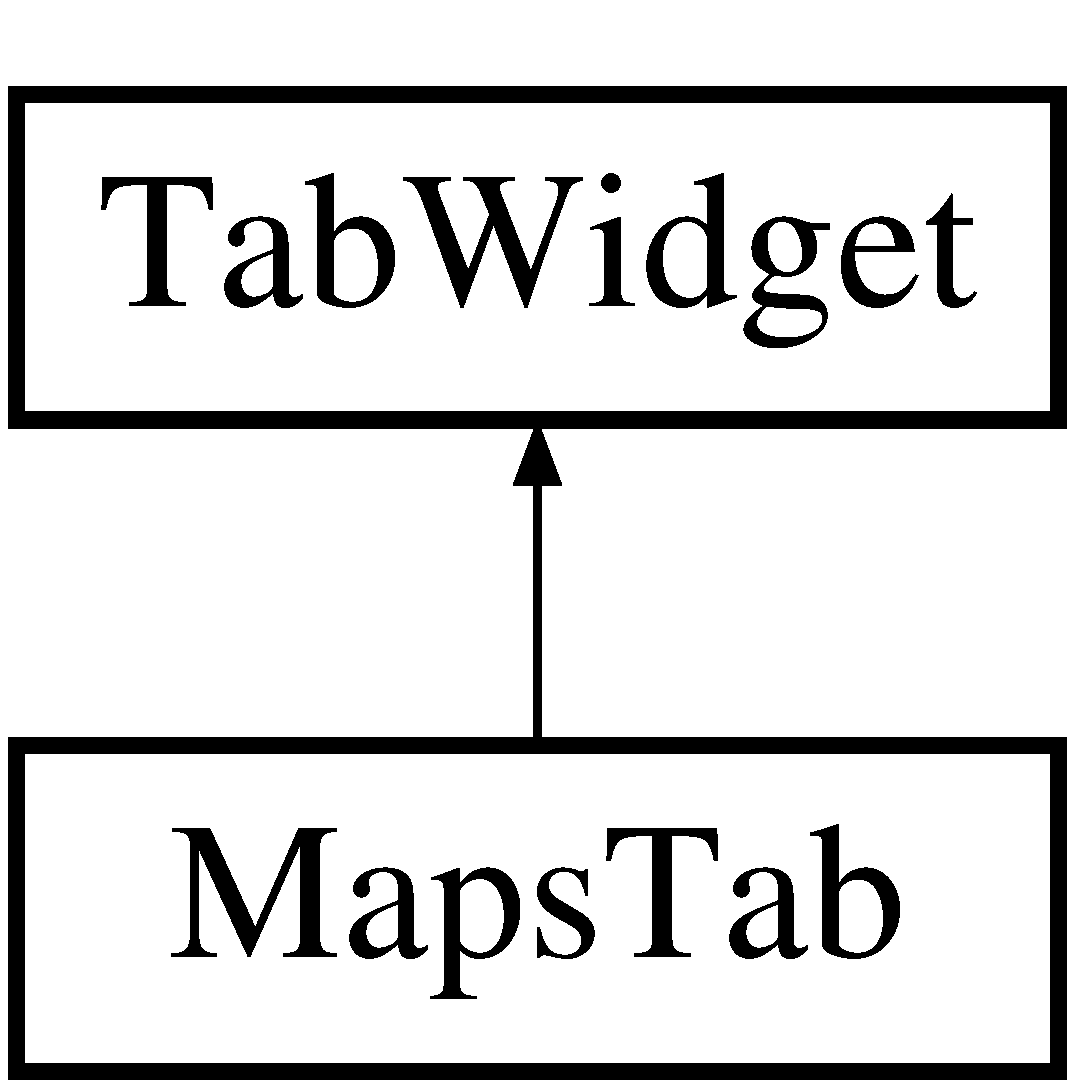
\includegraphics[height=2.000000cm]{class_maps_tab}
\end{center}
\end{figure}
\subsection*{\-Public \-Slots}
\begin{DoxyCompactItemize}
\item 
\hypertarget{class_maps_tab_a1983576710cfc5be47e8f8ffee580036}{void {\bfseries update\-Game} ()}\label{class_maps_tab_a1983576710cfc5be47e8f8ffee580036}

\end{DoxyCompactItemize}
\subsection*{\-Public \-Member \-Functions}
\begin{DoxyCompactItemize}
\item 
\hypertarget{class_maps_tab_a65f3887b8248421638a03a034a4ff8ed}{{\bfseries \-Maps\-Tab} (\-Q\-Widget $\ast$parent=0)}\label{class_maps_tab_a65f3887b8248421638a03a034a4ff8ed}

\item 
\hypertarget{class_maps_tab_ae5b95aa6d6ab4209655d79873b877e82}{void {\bfseries set\-Game} (\hyperlink{class_game}{\-Game} $\ast$g)}\label{class_maps_tab_ae5b95aa6d6ab4209655d79873b877e82}

\end{DoxyCompactItemize}


\subsection{\-Detailed \-Description}
\-The \-Map\-Tab class is the \hyperlink{class_tab_widget}{\-Tab\-Widget} that provides map edition features. 

\-The documentation for this class was generated from the following files\-:\begin{DoxyCompactItemize}
\item 
src/editor/\-G\-U\-I/\-Tabs/\-Map\-Tab/\hyperlink{maptab_8h}{maptab.\-h}\item 
src/editor/\-G\-U\-I/\-Tabs/\-Map\-Tab/maptab.\-cpp\end{DoxyCompactItemize}

\hypertarget{class_map_type}{\section{\-Map\-Type \-Class \-Reference}
\label{class_map_type}\index{\-Map\-Type@{\-Map\-Type}}
}


\-The \hyperlink{class_map_type}{\-Map\-Type} class defines the properties that are mandatory in any \hyperlink{class_map_type}{\-Map\-Type} object.  




{\ttfamily \#include $<$map.\-h$>$}

\-Inheritance diagram for \-Map\-Type\-:\begin{figure}[H]
\begin{center}
\leavevmode
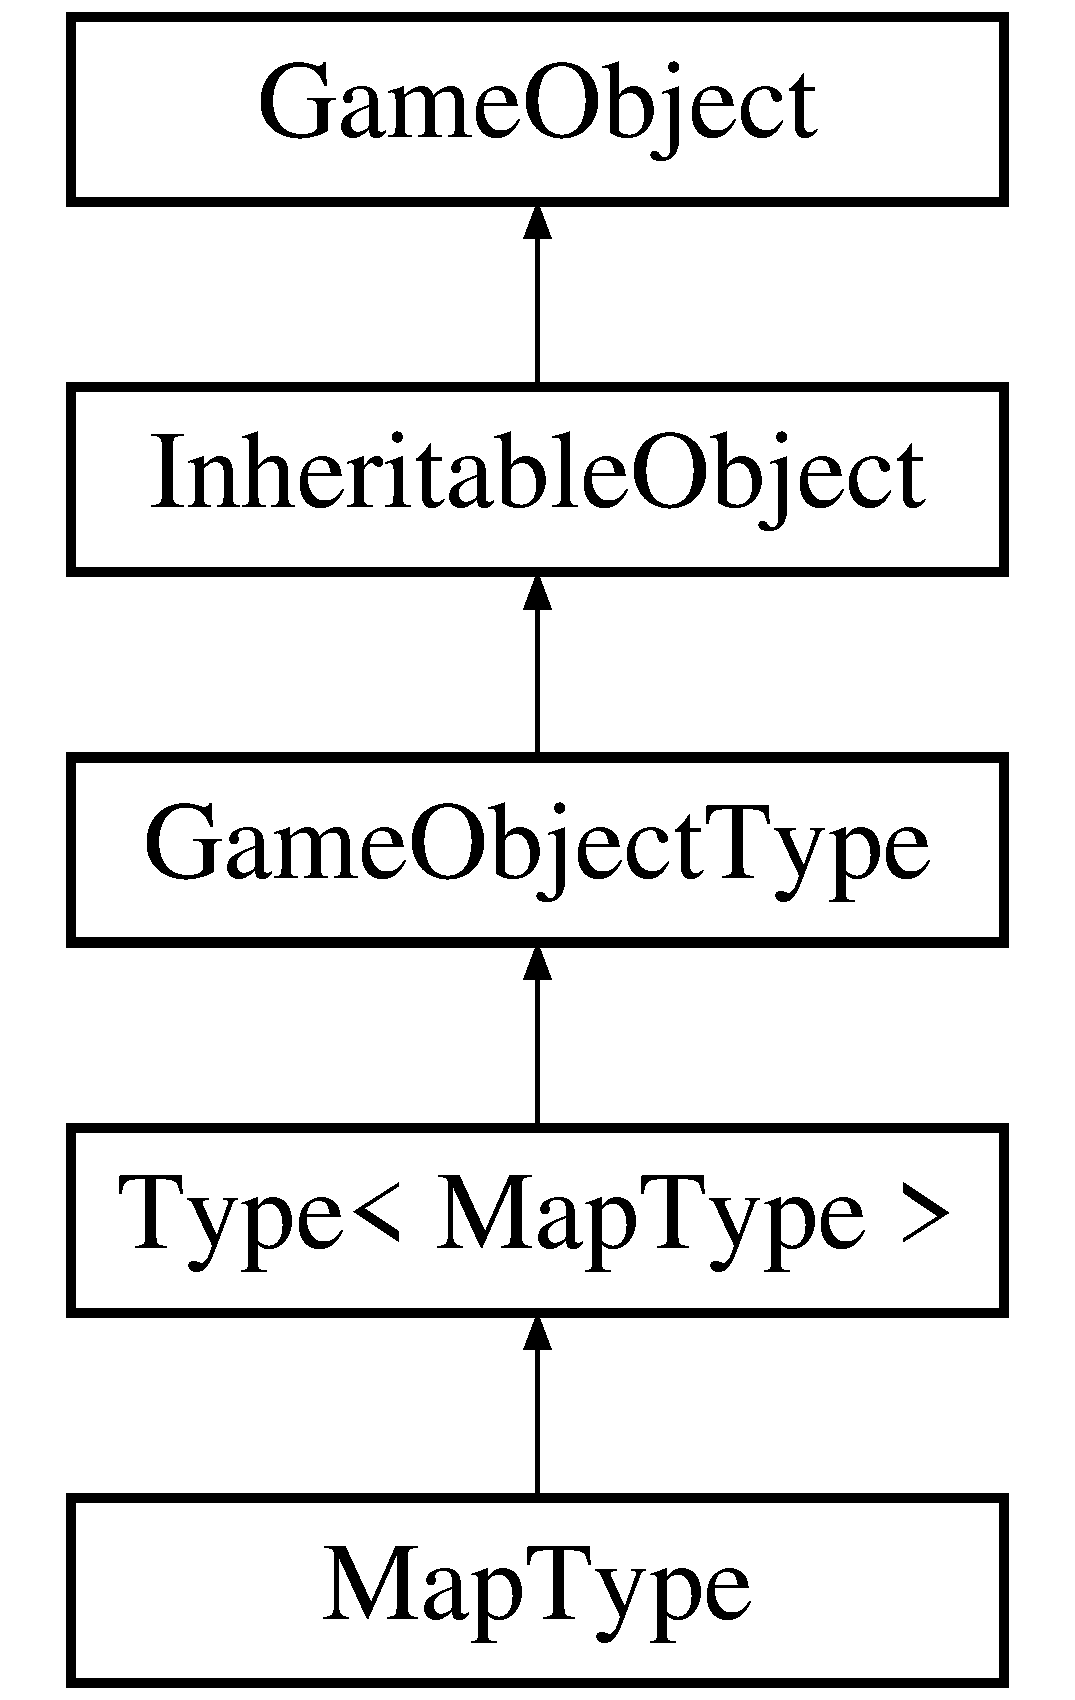
\includegraphics[height=5.000000cm]{class_map_type}
\end{center}
\end{figure}
\subsection*{\-Public \-Member \-Functions}
\begin{DoxyCompactItemize}
\item 
\hypertarget{class_map_type_aa2304487b4989920021c656d404ad893}{\hyperlink{class_map_type}{\-Map\-Type} {\bfseries \-Map\-Type} (\hyperlink{class_map_type}{\-Map\-Type} \&\hyperlink{class_inheritable_object_a10eead70368227b7f15f44f91d234fa5}{ancestor})}\label{class_map_type_aa2304487b4989920021c656d404ad893}

\item 
\hypertarget{class_map_type_affc4d021aa814cfc93096498b0395ba2}{{\bfseries \-Map\-Type} (\hyperlink{class_default_types}{\-Default\-Types} \&\hyperlink{class_game_object_af3deaf39cde23c189765634e32e95bb4}{parent})}\label{class_map_type_affc4d021aa814cfc93096498b0395ba2}

\end{DoxyCompactItemize}


\subsection{\-Detailed \-Description}
\-The \hyperlink{class_map_type}{\-Map\-Type} class defines the properties that are mandatory in any \hyperlink{class_map_type}{\-Map\-Type} object. 

\-The documentation for this class was generated from the following files\-:\begin{DoxyCompactItemize}
\item 
src/editor/\-Game/\hyperlink{map_8h}{map.\-h}\item 
src/editor/\-Game/map.\-cpp\end{DoxyCompactItemize}

\hypertarget{class_map_viewer}{\section{\-Map\-Viewer \-Class \-Reference}
\label{class_map_viewer}\index{\-Map\-Viewer@{\-Map\-Viewer}}
}


\-The \hyperlink{class_map_viewer}{\-Map\-Viewer} class provides a widget to display and edit a \hyperlink{class_map}{\-Map} using a \hyperlink{class_map_painter}{\-Map\-Painter}.  




{\ttfamily \#include $<$mapviewer.\-h$>$}

\subsection*{\-Public \-Slots}
\begin{DoxyCompactItemize}
\item 
\hypertarget{class_map_viewer_af6db4693f536ea5ce8b7b6f05d4099ea}{void {\bfseries update\-Request} ()}\label{class_map_viewer_af6db4693f536ea5ce8b7b6f05d4099ea}

\end{DoxyCompactItemize}
\subsection*{\-Signals}
\begin{DoxyCompactItemize}
\item 
\hypertarget{class_map_viewer_afe0db95f8db428737b5225663dd2b127}{void {\bfseries view\-Size\-Changed} (\-Q\-Size)}\label{class_map_viewer_afe0db95f8db428737b5225663dd2b127}

\item 
\hypertarget{class_map_viewer_a60b95fc5e6817673a532b11a139a0eab}{void {\bfseries selection\-Changed} ()}\label{class_map_viewer_a60b95fc5e6817673a532b11a139a0eab}

\end{DoxyCompactItemize}
\subsection*{\-Public \-Member \-Functions}
\begin{DoxyCompactItemize}
\item 
\hypertarget{class_map_viewer_ae2c78c6e6ac686b2db1f4b3a7e3f318a}{{\bfseries \-Map\-Viewer} (\-Q\-Widget $\ast$parent=0)}\label{class_map_viewer_ae2c78c6e6ac686b2db1f4b3a7e3f318a}

\item 
\hypertarget{class_map_viewer_a15df9bdd47e5ad36c67601d335bfa5f1}{void {\bfseries set\-Map} (\hyperlink{class_map}{\-Map} $\ast$m)}\label{class_map_viewer_a15df9bdd47e5ad36c67601d335bfa5f1}

\item 
\hypertarget{class_map_viewer_a723ad37abb7af9ecac0bdd68dd628e46}{void {\bfseries update\-Map} ()}\label{class_map_viewer_a723ad37abb7af9ecac0bdd68dd628e46}

\item 
\hypertarget{class_map_viewer_af30594b6df0ea90676a4dc4ec65abaca}{\hyperlink{class_map_painter}{\-Map\-Painter} \& {\bfseries map\-Painter} ()}\label{class_map_viewer_af30594b6df0ea90676a4dc4ec65abaca}

\end{DoxyCompactItemize}


\subsection{\-Detailed \-Description}
\-The \hyperlink{class_map_viewer}{\-Map\-Viewer} class provides a widget to display and edit a \hyperlink{class_map}{\-Map} using a \hyperlink{class_map_painter}{\-Map\-Painter}. 

\-The documentation for this class was generated from the following files\-:\begin{DoxyCompactItemize}
\item 
src/editor/\-G\-U\-I/\-Tabs/mapviewer.\-h\item 
src/editor/\-G\-U\-I/\-Tabs/mapviewer.\-cpp\end{DoxyCompactItemize}

\hypertarget{class_new_game}{\section{\-New\-Game \-Class \-Reference}
\label{class_new_game}\index{\-New\-Game@{\-New\-Game}}
}


\-The \hyperlink{class_new_game}{\-New\-Game} class provides a widget that defines the starting parameter for a new project.  




{\ttfamily \#include $<$newgame.\-h$>$}

\subsection*{\-Public \-Member \-Functions}
\begin{DoxyCompactItemize}
\item 
\hypertarget{class_new_game_abc0dccbe2a43eef32570473265de9a8a}{{\bfseries \-New\-Game} (\-Q\-Widget $\ast$parent=0)}\label{class_new_game_abc0dccbe2a43eef32570473265de9a8a}

\item 
\hypertarget{class_new_game_a7fd556a28c38e6c1c46ea227acad99bd}{\-Q\-String {\bfseries name} () const }\label{class_new_game_a7fd556a28c38e6c1c46ea227acad99bd}

\item 
\hypertarget{class_new_game_ae53e79a27fdd2b0610f5f98500f299cb}{\-Q\-String {\bfseries folder} () const }\label{class_new_game_ae53e79a27fdd2b0610f5f98500f299cb}

\item 
\hypertarget{class_new_game_a5f883cc09386cca3247acac873a36777}{bool {\bfseries create\-Folder} () const }\label{class_new_game_a5f883cc09386cca3247acac873a36777}

\end{DoxyCompactItemize}


\subsection{\-Detailed \-Description}
\-The \hyperlink{class_new_game}{\-New\-Game} class provides a widget that defines the starting parameter for a new project. 

\-The documentation for this class was generated from the following files\-:\begin{DoxyCompactItemize}
\item 
src/editor/\-G\-U\-I/\hyperlink{newgame_8h}{newgame.\-h}\item 
src/editor/\-G\-U\-I/newgame.\-cpp\end{DoxyCompactItemize}

\hypertarget{class_object}{\section{\-Object \-Class \-Reference}
\label{class_object}\index{\-Object@{\-Object}}
}


\-The \hyperlink{class_object}{\-Object} class.  




{\ttfamily \#include $<$object.\-h$>$}

\-Inheritance diagram for \-Object\-:\begin{figure}[H]
\begin{center}
\leavevmode
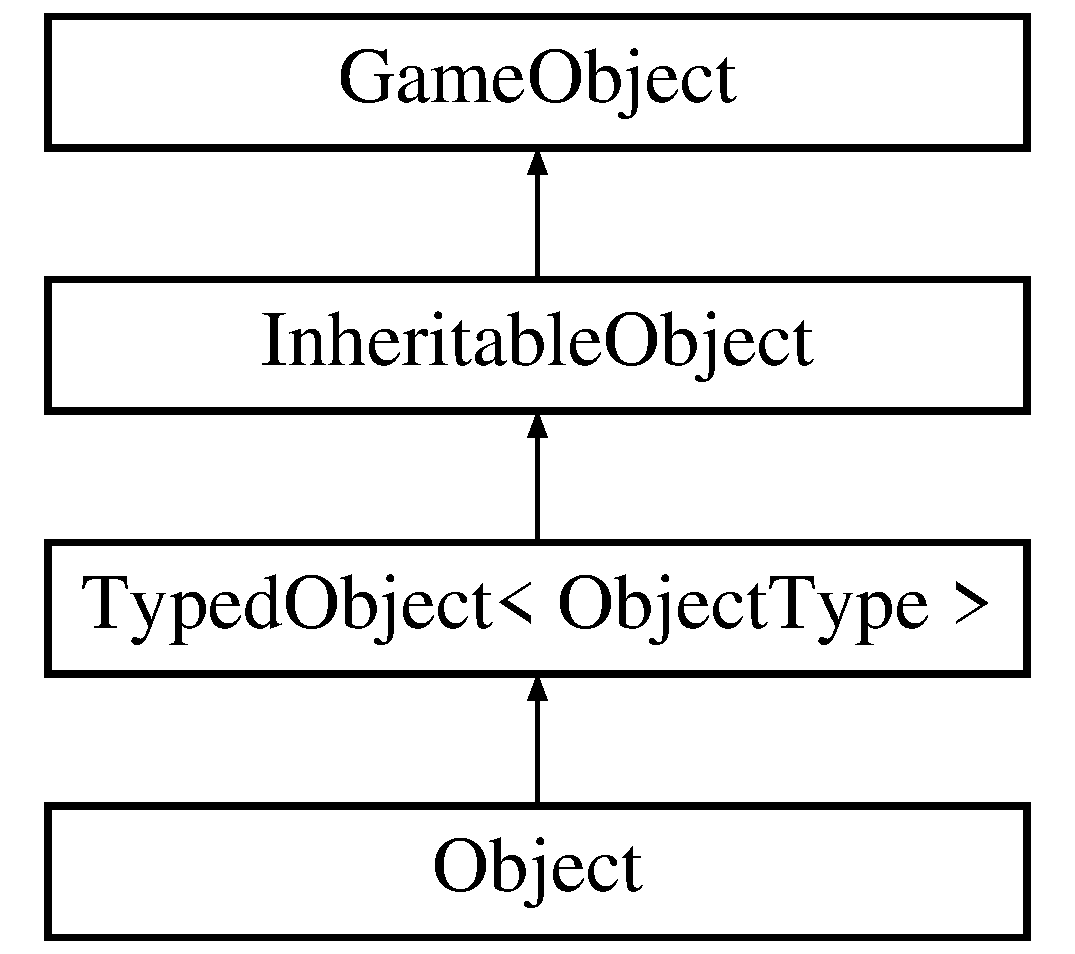
\includegraphics[height=4.000000cm]{class_object}
\end{center}
\end{figure}
\subsection*{\-Public \-Member \-Functions}
\begin{DoxyCompactItemize}
\item 
\hypertarget{class_object_ac0b6088495eae65bc1fd37c13423806a}{\hyperlink{class_object}{\-Object} {\bfseries \-Object} (\hyperlink{class_object_type}{\-Object\-Type} \&type, \hyperlink{class_game_object}{\-Game\-Object} \&\hyperlink{class_game_object_af3deaf39cde23c189765634e32e95bb4}{parent})}\label{class_object_ac0b6088495eae65bc1fd37c13423806a}

\item 
\hypertarget{class_object_ab0ea9f3d551da32c158b7cf791b622d0}{\hyperlink{class_object_type}{\-Object\-Type} \& {\bfseries object\-Type} ()}\label{class_object_ab0ea9f3d551da32c158b7cf791b622d0}

\end{DoxyCompactItemize}


\subsection{\-Detailed \-Description}
\-The \hyperlink{class_object}{\-Object} class. 

\-The documentation for this class was generated from the following files\-:\begin{DoxyCompactItemize}
\item 
src/editor/\-Game/\hyperlink{object_8h}{object.\-h}\item 
src/editor/\-Game/object.\-cpp\end{DoxyCompactItemize}

\hypertarget{class_object_name_item_delegate}{\section{\-Object\-Name\-Item\-Delegate \-Class \-Reference}
\label{class_object_name_item_delegate}\index{\-Object\-Name\-Item\-Delegate@{\-Object\-Name\-Item\-Delegate}}
}


\-The \hyperlink{class_object_name_item_delegate}{\-Object\-Name\-Item\-Delegate} class provides to view classes the way to modify object's name.  




{\ttfamily \#include $<$itemdelegates.\-h$>$}

\subsection*{\-Public \-Member \-Functions}
\begin{DoxyCompactItemize}
\item 
\hypertarget{class_object_name_item_delegate_a29ea6448c3b0db37a948cfb7802ce6b5}{{\bfseries \-Object\-Name\-Item\-Delegate} (\-Q\-Object $\ast$parent=nullptr)}\label{class_object_name_item_delegate_a29ea6448c3b0db37a948cfb7802ce6b5}

\item 
\hypertarget{class_object_name_item_delegate_a3e4e9d436c524a21953e61e0fcb9b798}{\-Q\-Widget $\ast$ {\bfseries create\-Editor} (\-Q\-Widget $\ast$parent, const \-Q\-Style\-Option\-View\-Item \&option, const \-Q\-Model\-Index \&index) const }\label{class_object_name_item_delegate_a3e4e9d436c524a21953e61e0fcb9b798}

\item 
\hypertarget{class_object_name_item_delegate_a97d0e306dd9de35e4db9074144b754e1}{void {\bfseries set\-Editor\-Data} (\-Q\-Widget $\ast$editor, const \-Q\-Model\-Index \&index) const }\label{class_object_name_item_delegate_a97d0e306dd9de35e4db9074144b754e1}

\item 
\hypertarget{class_object_name_item_delegate_a19c1f716cc9ae25eb428e2a8a976f6da}{void {\bfseries update\-Editor\-Geometry} (\-Q\-Widget $\ast$editor, const \-Q\-Style\-Option\-View\-Item \&option, const \-Q\-Model\-Index \&index) const }\label{class_object_name_item_delegate_a19c1f716cc9ae25eb428e2a8a976f6da}

\item 
\hypertarget{class_object_name_item_delegate_a8b30c82a50aedb27bdfc34489ae09809}{void {\bfseries paint} (\-Q\-Painter $\ast$painter, const \-Q\-Style\-Option\-View\-Item \&option, const \-Q\-Model\-Index \&index) const }\label{class_object_name_item_delegate_a8b30c82a50aedb27bdfc34489ae09809}

\end{DoxyCompactItemize}


\subsection{\-Detailed \-Description}
\-The \hyperlink{class_object_name_item_delegate}{\-Object\-Name\-Item\-Delegate} class provides to view classes the way to modify object's name. 

\-The documentation for this class was generated from the following files\-:\begin{DoxyCompactItemize}
\item 
src/editor/\-G\-U\-I/\-Tabs/\hyperlink{itemdelegates_8h}{itemdelegates.\-h}\item 
src/editor/\-G\-U\-I/\-Tabs/itemdelegates.\-cpp\end{DoxyCompactItemize}

\hypertarget{class_objects_tree_model}{\section{\-Objects\-Tree\-Model \-Class \-Reference}
\label{class_objects_tree_model}\index{\-Objects\-Tree\-Model@{\-Objects\-Tree\-Model}}
}


\-The \hyperlink{class_objects_tree_model}{\-Objects\-Tree\-Model} class presents an \hyperlink{class_game_object}{\-Game\-Object} and its chidren as a tree model.  




{\ttfamily \#include $<$itemmodels.\-h$>$}

\subsection*{\-Public \-Member \-Functions}
\begin{DoxyCompactItemize}
\item 
\hypertarget{class_objects_tree_model_a4cc5d9d4f4a979715d93841b8d76c996}{{\bfseries \-Objects\-Tree\-Model} (\-Q\-Object $\ast$parent=nullptr)}\label{class_objects_tree_model_a4cc5d9d4f4a979715d93841b8d76c996}

\item 
\hypertarget{class_objects_tree_model_a5661982a1cc727ac0961e2961395fb96}{{\bfseries \-Objects\-Tree\-Model} (\hyperlink{class_game_object}{\-Game\-Object} $\ast$o, \-Q\-Object $\ast$parent=nullptr)}\label{class_objects_tree_model_a5661982a1cc727ac0961e2961395fb96}

\item 
\hypertarget{class_objects_tree_model_a009ac110d33747aff36bd5ab1e07211a}{void {\bfseries set\-Game\-Object} (\hyperlink{class_game_object}{\-Game\-Object} $\ast$o)}\label{class_objects_tree_model_a009ac110d33747aff36bd5ab1e07211a}

\item 
\hypertarget{class_objects_tree_model_a41005844e75c80f30b638b50d36653c4}{int {\bfseries column\-Count} (const \-Q\-Model\-Index \&) const }\label{class_objects_tree_model_a41005844e75c80f30b638b50d36653c4}

\item 
\hypertarget{class_objects_tree_model_aa7740390e180a7663e3341a5aa56c49b}{int {\bfseries row\-Count} (const \-Q\-Model\-Index \&parent) const }\label{class_objects_tree_model_aa7740390e180a7663e3341a5aa56c49b}

\item 
\hypertarget{class_objects_tree_model_a98fe0687618c87c84f5519c92d729aa0}{\-Q\-Variant {\bfseries data} (const \-Q\-Model\-Index \&index, int role) const }\label{class_objects_tree_model_a98fe0687618c87c84f5519c92d729aa0}

\item 
\hypertarget{class_objects_tree_model_a8c9f9980e0268c7125f97ce9e45e026d}{\-Q\-Model\-Index {\bfseries index} (int row, int column, const \-Q\-Model\-Index \&parent) const }\label{class_objects_tree_model_a8c9f9980e0268c7125f97ce9e45e026d}

\item 
\hypertarget{class_objects_tree_model_a304b4e2110a7ab9e697d1ace64885792}{\-Q\-Model\-Index {\bfseries parent} (const \-Q\-Model\-Index \&child) const }\label{class_objects_tree_model_a304b4e2110a7ab9e697d1ace64885792}

\item 
\hypertarget{class_objects_tree_model_ae8574c384005c730762b083eb3863d74}{\-Q\-Variant {\bfseries header\-Data} (int section, \-Qt\-::\-Orientation orientation, int role) const }\label{class_objects_tree_model_ae8574c384005c730762b083eb3863d74}

\item 
\hypertarget{class_objects_tree_model_a7cbd6321c7f581a088d0e93418724898}{\-Qt\-::\-Item\-Flags {\bfseries flags} (const \-Q\-Model\-Index \&index) const }\label{class_objects_tree_model_a7cbd6321c7f581a088d0e93418724898}

\item 
\hypertarget{class_objects_tree_model_a33316c0c59125afb510d7df5d62784a4}{bool {\bfseries set\-Data} (const \-Q\-Model\-Index \&index, const \-Q\-Variant \&value, int role)}\label{class_objects_tree_model_a33316c0c59125afb510d7df5d62784a4}

\item 
\hypertarget{class_objects_tree_model_a39fa12bae610f2ff38250aac4633ce20}{void {\bfseries set\-Editable} (bool e)}\label{class_objects_tree_model_a39fa12bae610f2ff38250aac4633ce20}

\item 
\hypertarget{class_objects_tree_model_a98d3d2ed8e827ac26baf88ef6ac564ba}{\-Q\-Model\-Index {\bfseries find} (int id, const \-Q\-Model\-Index \&root=\-Q\-Model\-Index())}\label{class_objects_tree_model_a98d3d2ed8e827ac26baf88ef6ac564ba}

\end{DoxyCompactItemize}


\subsection{\-Detailed \-Description}
\-The \hyperlink{class_objects_tree_model}{\-Objects\-Tree\-Model} class presents an \hyperlink{class_game_object}{\-Game\-Object} and its chidren as a tree model. 

\-The documentation for this class was generated from the following files\-:\begin{DoxyCompactItemize}
\item 
src/editor/\-Game/\-Item\-Models/\hyperlink{itemmodels_8h}{itemmodels.\-h}\item 
src/editor/\-Game/\-Item\-Models/itemmodels.\-cpp\end{DoxyCompactItemize}

\hypertarget{class_object_tab}{\section{\-Object\-Tab \-Class \-Reference}
\label{class_object_tab}\index{\-Object\-Tab@{\-Object\-Tab}}
}


\-The \hyperlink{class_object_tab}{\-Object\-Tab} class is the \hyperlink{class_tab_widget}{\-Tab\-Widget} that provides object edition features.  




{\ttfamily \#include $<$objecttab.\-h$>$}

\-Inheritance diagram for \-Object\-Tab\-:\begin{figure}[H]
\begin{center}
\leavevmode
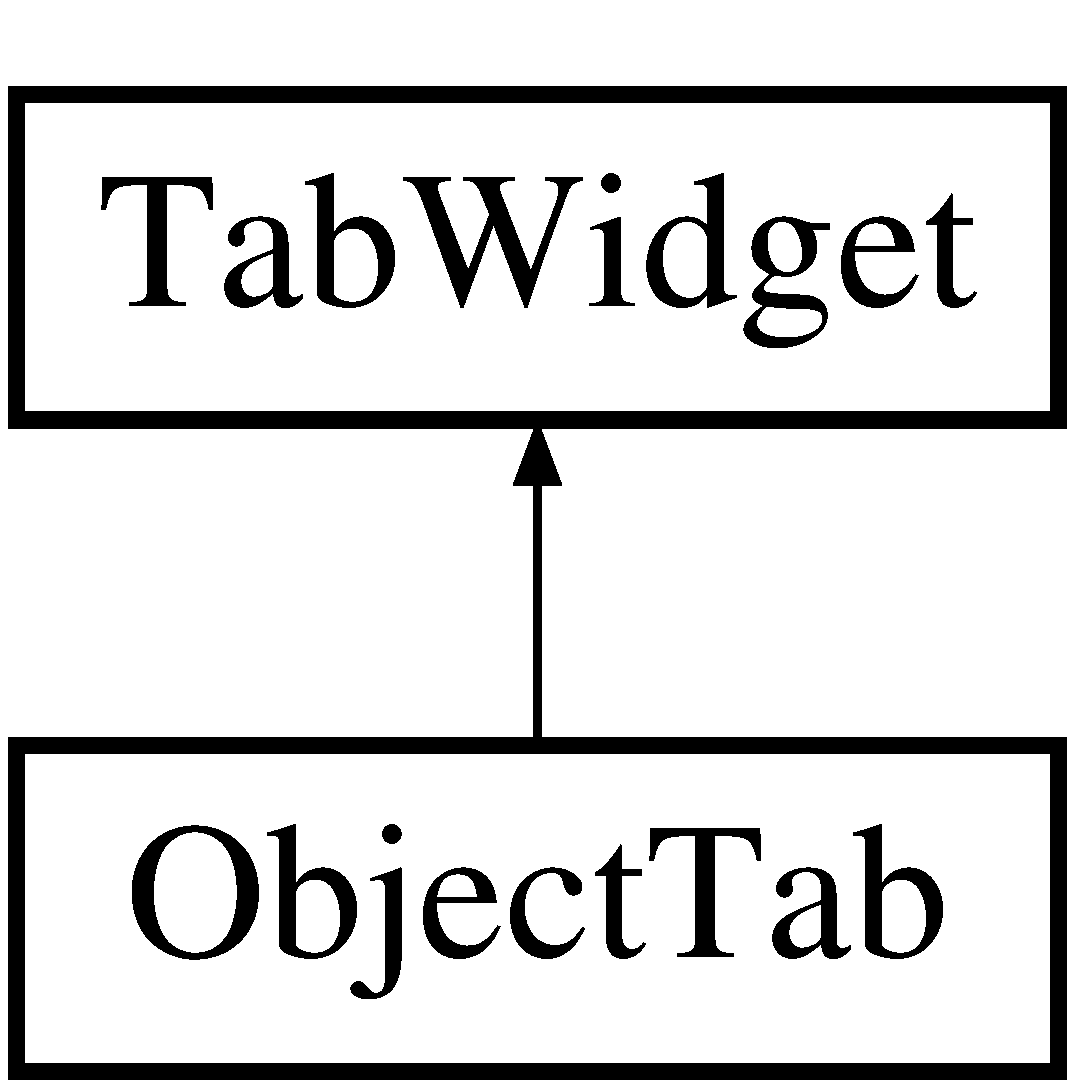
\includegraphics[height=2.000000cm]{class_object_tab}
\end{center}
\end{figure}
\subsection*{\-Public \-Member \-Functions}
\begin{DoxyCompactItemize}
\item 
\hypertarget{class_object_tab_acf791488320fd040c1a04065abae73d3}{{\bfseries \-Object\-Tab} (\-Q\-Widget $\ast$parent=0)}\label{class_object_tab_acf791488320fd040c1a04065abae73d3}

\item 
\hypertarget{class_object_tab_a41031bc268bd880d0b08c0feb6fa8ac4}{void {\bfseries set\-Game} (\hyperlink{class_game}{\-Game} $\ast$g)}\label{class_object_tab_a41031bc268bd880d0b08c0feb6fa8ac4}

\end{DoxyCompactItemize}


\subsection{\-Detailed \-Description}
\-The \hyperlink{class_object_tab}{\-Object\-Tab} class is the \hyperlink{class_tab_widget}{\-Tab\-Widget} that provides object edition features. 

\-The documentation for this class was generated from the following files\-:\begin{DoxyCompactItemize}
\item 
src/editor/\-G\-U\-I/\-Tabs/\hyperlink{objecttab_8h}{objecttab.\-h}\item 
src/editor/\-G\-U\-I/\-Tabs/objecttab.\-cpp\end{DoxyCompactItemize}

\hypertarget{class_object_type}{\section{\-Object\-Type \-Class \-Reference}
\label{class_object_type}\index{\-Object\-Type@{\-Object\-Type}}
}


\-The \hyperlink{class_object_type}{\-Object\-Type} class defines the properties that are mandatory in any \hyperlink{class_object_type}{\-Object\-Type} object.  




{\ttfamily \#include $<$object.\-h$>$}

\-Inheritance diagram for \-Object\-Type\-:\begin{figure}[H]
\begin{center}
\leavevmode
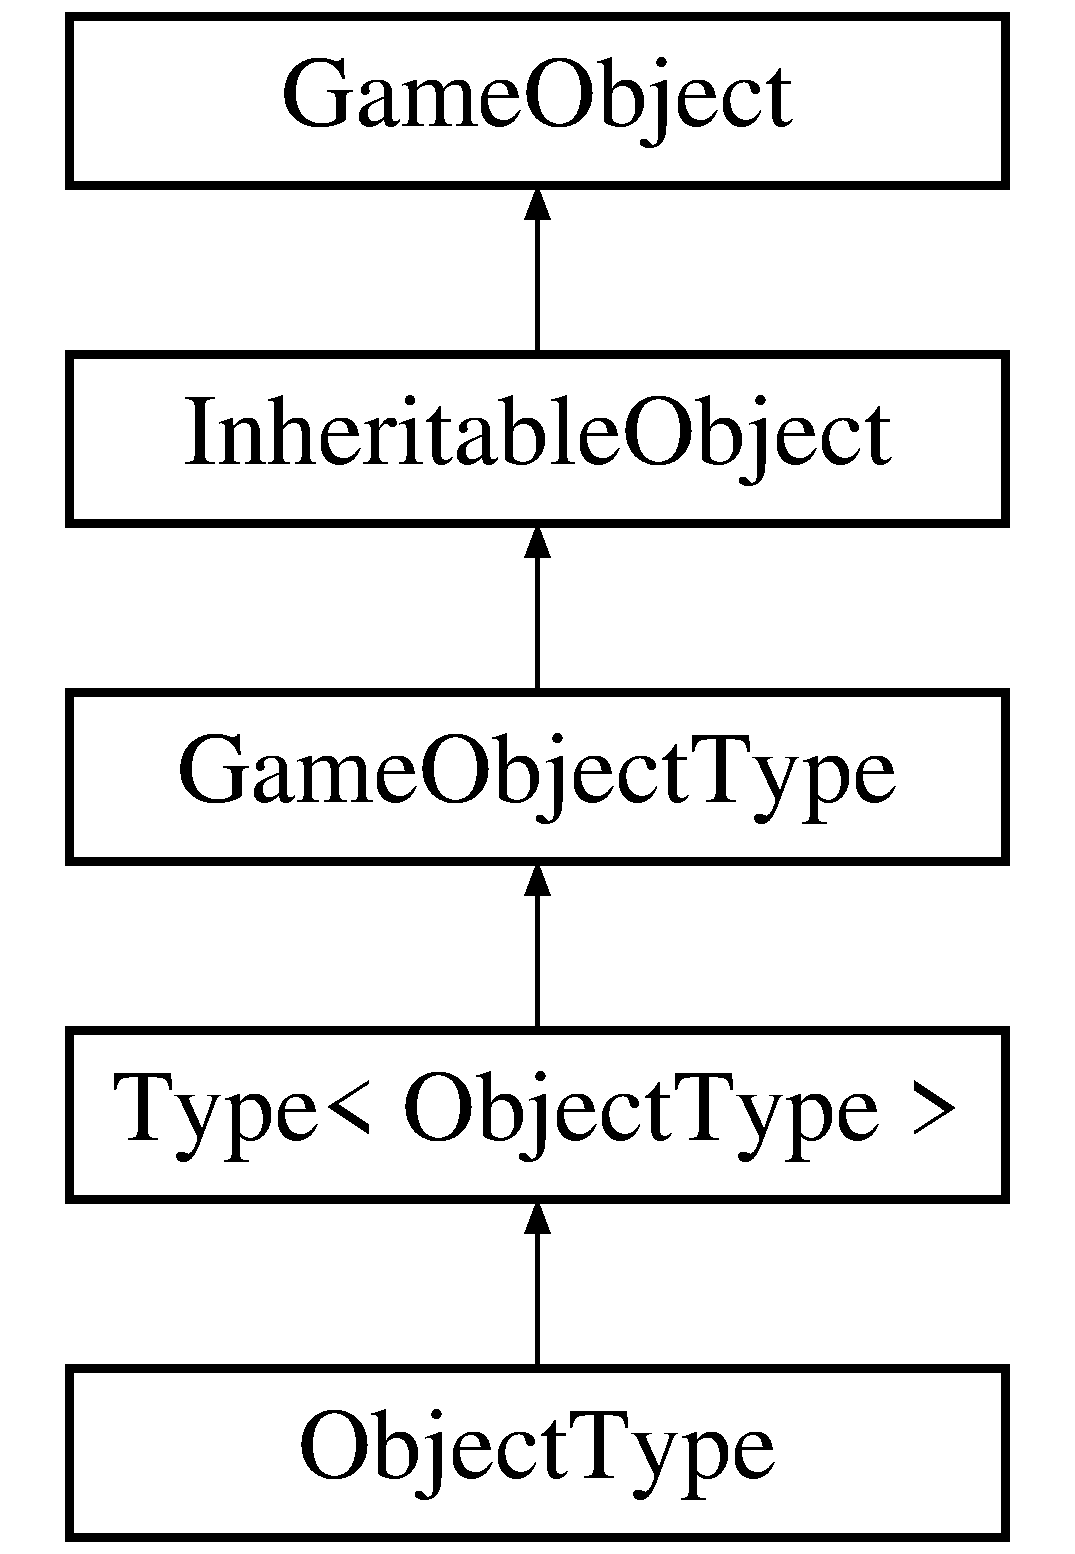
\includegraphics[height=5.000000cm]{class_object_type}
\end{center}
\end{figure}
\subsection*{\-Public \-Member \-Functions}
\begin{DoxyCompactItemize}
\item 
\hypertarget{class_object_type_a331d8b3f8f0cefa4c1806d5005ab39fb}{\hyperlink{class_object_type}{\-Object\-Type} {\bfseries \-Object\-Type} (\hyperlink{class_object_type}{\-Object\-Type} \&\hyperlink{class_inheritable_object_a10eead70368227b7f15f44f91d234fa5}{ancestor})}\label{class_object_type_a331d8b3f8f0cefa4c1806d5005ab39fb}

\item 
\hypertarget{class_object_type_ab0c8f836fb9a204d6a8c5fc430988135}{{\bfseries \-Object\-Type} (\hyperlink{class_default_types}{\-Default\-Types} \&\hyperlink{class_game_object_af3deaf39cde23c189765634e32e95bb4}{parent})}\label{class_object_type_ab0c8f836fb9a204d6a8c5fc430988135}

\item 
\hypertarget{class_object_type_ad69430f792b80dc4dbbf52e42a956fb1}{\hyperlink{class_image}{\-Image} $\ast$ {\bfseries image} () const }\label{class_object_type_ad69430f792b80dc4dbbf52e42a956fb1}

\item 
\hypertarget{class_object_type_a645e1893d343dc9ba1a9c667cc6f0d36}{void {\bfseries set\-Image} (\hyperlink{class_image}{\-Image} $\ast$im)}\label{class_object_type_a645e1893d343dc9ba1a9c667cc6f0d36}

\end{DoxyCompactItemize}


\subsection{\-Detailed \-Description}
\-The \hyperlink{class_object_type}{\-Object\-Type} class defines the properties that are mandatory in any \hyperlink{class_object_type}{\-Object\-Type} object. 

\-The documentation for this class was generated from the following files\-:\begin{DoxyCompactItemize}
\item 
src/editor/\-Game/\hyperlink{object_8h}{object.\-h}\item 
src/editor/\-Game/object.\-cpp\end{DoxyCompactItemize}

\hypertarget{struct_options}{\section{\-Options \-Struct \-Reference}
\label{struct_options}\index{\-Options@{\-Options}}
}


\-The \hyperlink{struct_options}{\-Options} class provides session-\/independant options and preferences.  




{\ttfamily \#include $<$options.\-h$>$}

\subsection*{\-Public \-Member \-Functions}
\begin{DoxyCompactItemize}
\item 
{\footnotesize template$<$class T $>$ }\\\-T \hyperlink{struct_options_ada32d485296bd6ba73a1d95bd6260c1a}{load} (\-Q\-String group, \-Q\-String opt)
\item 
{\footnotesize template$<$class T $>$ }\\void \hyperlink{struct_options_ad20146ff9544f6229bb1696ea5bf643d}{save} (\-Q\-String group, \-Q\-String opt, \-T val)
\item 
{\footnotesize template$<$class T $>$ }\\void \hyperlink{struct_options_ab1d167bd93bce7dd453fcbb93acf12e4}{set\-Default} (\-Q\-String group, \-Q\-String opt, \-T val)
\item 
bool \hyperlink{struct_options_a1188a188db82d70c96af44679d2cbbf9}{is\-Adjustable} (\-Q\-String group, \-Q\-String opt, bool adjust=true)
\item 
void \hyperlink{struct_options_a086db8fe7688ddcb3b74db85262a5ba0}{set\-Adjustable} (\-Q\-String group, \-Q\-String opt, bool adjust)
\item 
void \hyperlink{struct_options_a336da0a8bbd1b849a1783bb110904d9f}{reinitialise} (\-Q\-String group=\char`\"{}\char`\"{})
\end{DoxyCompactItemize}
\subsection*{\-Static \-Public \-Member \-Functions}
\begin{DoxyCompactItemize}
\item 
static \hyperlink{struct_options}{\-Options} \& \hyperlink{struct_options_aa3dd7609fbc5d54af65992632bff842a}{options} ()
\end{DoxyCompactItemize}


\subsection{\-Detailed \-Description}
\-The \hyperlink{struct_options}{\-Options} class provides session-\/independant options and preferences. 

\#\# \-Features

\-The \hyperlink{struct_options}{\-Options} class aims at storing global options, that are available at any place in the entire application. \-The preferences are permanantly stored and remain bewteen the separate sessions and windows.

\-Two sorts of options exist \-:
\begin{DoxyItemize}
\item \-The adjustable ones \-: the value of the option change when \hyperlink{struct_options_ad20146ff9544f6229bb1696ea5bf643d}{save} is called.
\item \-The non-\/adjustable ones \-: the value of the option doesn't change is \hyperlink{struct_options_ad20146ff9544f6229bb1696ea5bf643d}{save} is called, the option must be modified with .
\end{DoxyItemize}

\-The sort of option can be set with the \hyperlink{struct_options_a086db8fe7688ddcb3b74db85262a5ba0}{set\-Adjustable} function.

\#\# \-Design

\-The \hyperlink{struct_options}{\-Options} class is designed following the \-\_\-\-\_\-\-Singleton design pattern\-\_\-\-\_\-. \-The constructor is thus private, and the only \hyperlink{struct_options}{\-Options} instance is created at the first call of \hyperlink{struct_options_aa3dd7609fbc5d54af65992632bff842a}{options}.

\-Q\-Setting is used internaly, see \-Qt's documentation for details about the storing mechanisms.

\#\# \-Reading and writting existing options

\-To read or write options, the \hyperlink{struct_options}{\-Options} instance must be retreived, using the \hyperlink{struct_options_aa3dd7609fbc5d54af65992632bff842a}{options} function, then the \hyperlink{struct_options_ada32d485296bd6ba73a1d95bd6260c1a}{load} and \hyperlink{struct_options_ad20146ff9544f6229bb1696ea5bf643d}{save} functions can be called.

\#\# \-Adding options

\-To add a new option, it is only needed to add a default hard coded value, uisng the \hyperlink{options_8h_a37c44b1e71afed084dbe855181c444e2}{\-Default} and \hyperlink{options_8h_a39f3ee28f306ee663a9985433ef2d01c}{\-Default\-F} macros in the \hyperlink{struct_options}{\-Options} constructor.

\-It is strongly advice to use macro to define new options group (see \hyperlink{options_8h_a43105771f16e2da3078149f0de528e9b}{\-W\-I\-N}, for an example).

\begin{DoxyNote}{\-Note}
\-To use \hyperlink{struct_options}{\-Options} with custom types (other than ```\-C++``` standard), the defining header of the type must be included at the top of the \hyperlink{options_8h}{options.\-h} file, in order to be used in the default value declaration.
\end{DoxyNote}
\begin{DoxyWarning}{\-Warning}
\-Pointer objects are not supported, and the result of the use of the \hyperlink{struct_options}{\-Options} class with such values is undefined.
\end{DoxyWarning}
\begin{DoxySeeAlso}{\-See also}
\hyperlink{options_8h}{options.\-h} 
\end{DoxySeeAlso}


\subsection{\-Member \-Function \-Documentation}
\hypertarget{struct_options_a1188a188db82d70c96af44679d2cbbf9}{\index{\-Options@{\-Options}!is\-Adjustable@{is\-Adjustable}}
\index{is\-Adjustable@{is\-Adjustable}!Options@{\-Options}}
\subsubsection[{is\-Adjustable}]{\setlength{\rightskip}{0pt plus 5cm}bool {\bf \-Options\-::is\-Adjustable} (
\begin{DoxyParamCaption}
\item[{\-Q\-String}]{group, }
\item[{\-Q\-String}]{opt, }
\item[{bool}]{adjust = {\ttfamily true}}
\end{DoxyParamCaption}
)}}\label{struct_options_a1188a188db82d70c96af44679d2cbbf9}
\-Returns ```true``` if the option defined by its group and name is adjustable, ```false``` elsewhere.

\begin{DoxySeeAlso}{\-See also}
\hyperlink{struct_options_a086db8fe7688ddcb3b74db85262a5ba0}{set\-Adjustable} 
\end{DoxySeeAlso}
\hypertarget{struct_options_ada32d485296bd6ba73a1d95bd6260c1a}{\index{\-Options@{\-Options}!load@{load}}
\index{load@{load}!Options@{\-Options}}
\subsubsection[{load}]{\setlength{\rightskip}{0pt plus 5cm}template$<$class T $>$ \-T {\bf \-Options\-::load} (
\begin{DoxyParamCaption}
\item[{\-Q\-String}]{group, }
\item[{\-Q\-String}]{opt}
\end{DoxyParamCaption}
)\hspace{0.3cm}{\ttfamily  \mbox{[}inline\mbox{]}}}}\label{struct_options_ada32d485296bd6ba73a1d95bd6260c1a}
\-Reads an option defined by its group and name.

\begin{DoxyNote}{\-Note}
\-The template argument must be precised since it can't be deduced from arguments' types.
\end{DoxyNote}
\begin{DoxyWarning}{\-Warning}
\-If the option type and the reading type mismatch, an default null value is returned.
\end{DoxyWarning}
\begin{DoxySeeAlso}{\-See also}
\hyperlink{struct_options_ad20146ff9544f6229bb1696ea5bf643d}{save} 
\end{DoxySeeAlso}
\hypertarget{struct_options_aa3dd7609fbc5d54af65992632bff842a}{\index{\-Options@{\-Options}!options@{options}}
\index{options@{options}!Options@{\-Options}}
\subsubsection[{options}]{\setlength{\rightskip}{0pt plus 5cm}{\bf \-Options} \& {\bf \-Options\-::options} (
\begin{DoxyParamCaption}
{}
\end{DoxyParamCaption}
)\hspace{0.3cm}{\ttfamily  \mbox{[}static\mbox{]}}}}\label{struct_options_aa3dd7609fbc5d54af65992632bff842a}
\-Returns the unique \hyperlink{struct_options}{\-Options} instance. \hypertarget{struct_options_a336da0a8bbd1b849a1783bb110904d9f}{\index{\-Options@{\-Options}!reinitialise@{reinitialise}}
\index{reinitialise@{reinitialise}!Options@{\-Options}}
\subsubsection[{reinitialise}]{\setlength{\rightskip}{0pt plus 5cm}void {\bf \-Options\-::reinitialise} (
\begin{DoxyParamCaption}
\item[{\-Q\-String}]{group = {\ttfamily \char`\"{}\char`\"{}}}
\end{DoxyParamCaption}
)}}\label{struct_options_a336da0a8bbd1b849a1783bb110904d9f}
\-Clear all options from the group. \-If ```group == \char`\"{}\char`\"{}```, all entries are deleted. \hypertarget{struct_options_ad20146ff9544f6229bb1696ea5bf643d}{\index{\-Options@{\-Options}!save@{save}}
\index{save@{save}!Options@{\-Options}}
\subsubsection[{save}]{\setlength{\rightskip}{0pt plus 5cm}template$<$class T $>$ void {\bf \-Options\-::save} (
\begin{DoxyParamCaption}
\item[{\-Q\-String}]{group, }
\item[{\-Q\-String}]{opt, }
\item[{\-T}]{val}
\end{DoxyParamCaption}
)\hspace{0.3cm}{\ttfamily  \mbox{[}inline\mbox{]}}}}\label{struct_options_ad20146ff9544f6229bb1696ea5bf643d}
\-Writes the new value of the options defined by its group and name, if the option is adjustable. \-See \hyperlink{struct_options}{\-Options} for details about options types.

\begin{DoxyNote}{\-Note}
\-The template argument can be omitted since it would be deduced from the value argument.
\end{DoxyNote}
\begin{DoxySeeAlso}{\-See also}
\hyperlink{struct_options_ab1d167bd93bce7dd453fcbb93acf12e4}{set\-Default}, \hyperlink{struct_options_ada32d485296bd6ba73a1d95bd6260c1a}{load} 
\end{DoxySeeAlso}
\hypertarget{struct_options_a086db8fe7688ddcb3b74db85262a5ba0}{\index{\-Options@{\-Options}!set\-Adjustable@{set\-Adjustable}}
\index{set\-Adjustable@{set\-Adjustable}!Options@{\-Options}}
\subsubsection[{set\-Adjustable}]{\setlength{\rightskip}{0pt plus 5cm}void {\bf \-Options\-::set\-Adjustable} (
\begin{DoxyParamCaption}
\item[{\-Q\-String}]{group, }
\item[{\-Q\-String}]{opt, }
\item[{bool}]{adjust}
\end{DoxyParamCaption}
)}}\label{struct_options_a086db8fe7688ddcb3b74db85262a5ba0}
\-Sets if the option defined by its group and name is adjustable.

\begin{DoxySeeAlso}{\-See also}
\hyperlink{struct_options_a1188a188db82d70c96af44679d2cbbf9}{is\-Adjustable} 
\end{DoxySeeAlso}
\hypertarget{struct_options_ab1d167bd93bce7dd453fcbb93acf12e4}{\index{\-Options@{\-Options}!set\-Default@{set\-Default}}
\index{set\-Default@{set\-Default}!Options@{\-Options}}
\subsubsection[{set\-Default}]{\setlength{\rightskip}{0pt plus 5cm}template$<$class T $>$ void {\bf \-Options\-::set\-Default} (
\begin{DoxyParamCaption}
\item[{\-Q\-String}]{group, }
\item[{\-Q\-String}]{opt, }
\item[{\-T}]{val}
\end{DoxyParamCaption}
)\hspace{0.3cm}{\ttfamily  \mbox{[}inline\mbox{]}}}}\label{struct_options_ab1d167bd93bce7dd453fcbb93acf12e4}
\-Writes the new value of the options defined by its group and name, whatever the option type is. \-See \hyperlink{struct_options}{\-Options} for details about options types.

\begin{DoxyNote}{\-Note}
\-The template argument can be omitted since it would be deduced from the value argument.
\end{DoxyNote}
\begin{DoxySeeAlso}{\-See also}
\hyperlink{struct_options_ad20146ff9544f6229bb1696ea5bf643d}{save}, \hyperlink{struct_options_ada32d485296bd6ba73a1d95bd6260c1a}{load} 
\end{DoxySeeAlso}


\-The documentation for this struct was generated from the following files\-:\begin{DoxyCompactItemize}
\item 
src/editor/\-G\-U\-I/\hyperlink{options_8h}{options.\-h}\item 
src/editor/\-G\-U\-I/options.\-cpp\end{DoxyCompactItemize}

\hypertarget{class_parameter}{\section{\-Parameter \-Class \-Reference}
\label{class_parameter}\index{\-Parameter@{\-Parameter}}
}


\-The \hyperlink{class_parameter}{\-Parameter} class represents a parameter with a valid domain of value.  




{\ttfamily \#include $<$gameobject.\-h$>$}

\subsection*{\-Public \-Member \-Functions}
\begin{DoxyCompactItemize}
\item 
\hypertarget{class_parameter_aa6c9e61f1bb69049360de0d3eb87a365}{{\bfseries \-Parameter} (int v=0)}\label{class_parameter_aa6c9e61f1bb69049360de0d3eb87a365}

\item 
\hypertarget{class_parameter_a161c8aa0045e72afea7fe3bc3c1882c4}{{\bfseries \-Parameter} (int min, int max, int v=0)}\label{class_parameter_a161c8aa0045e72afea7fe3bc3c1882c4}

\item 
\hypertarget{class_parameter_a5f4ec5f133fc90d0b20e83a063f5eb5c}{void {\bfseries set\-Value} (int v)}\label{class_parameter_a5f4ec5f133fc90d0b20e83a063f5eb5c}

\item 
\hypertarget{class_parameter_a971c0369e19300bf5f38124964203a65}{int {\bfseries value} () const }\label{class_parameter_a971c0369e19300bf5f38124964203a65}

\item 
\hypertarget{class_parameter_a8618a13484e3a4c6ef36cabe85bb6c23}{void {\bfseries set\-Minimum} (int m)}\label{class_parameter_a8618a13484e3a4c6ef36cabe85bb6c23}

\item 
\hypertarget{class_parameter_a181c5a830f3ee9c5a08eb62f7f678212}{int {\bfseries minimum} () const }\label{class_parameter_a181c5a830f3ee9c5a08eb62f7f678212}

\item 
\hypertarget{class_parameter_ac5566dd445d208c138fc3f4510866959}{void {\bfseries set\-Maximum} (int m)}\label{class_parameter_ac5566dd445d208c138fc3f4510866959}

\item 
\hypertarget{class_parameter_afad0d040faf31c5faeaf63cd5cf048c8}{int {\bfseries maximum} () const }\label{class_parameter_afad0d040faf31c5faeaf63cd5cf048c8}

\item 
\hypertarget{class_parameter_a0a239a5f6f32ca67ef601730f5aa2e6d}{void {\bfseries set\-Domain} (int min\-Val, int max\-Val)}\label{class_parameter_a0a239a5f6f32ca67ef601730f5aa2e6d}

\end{DoxyCompactItemize}


\subsection{\-Detailed \-Description}
\-The \hyperlink{class_parameter}{\-Parameter} class represents a parameter with a valid domain of value. 

\-The documentation for this class was generated from the following file\-:\begin{DoxyCompactItemize}
\item 
src/editor/\-Game/\hyperlink{gameobject_8h}{gameobject.\-h}\end{DoxyCompactItemize}

\hypertarget{class_param_item_delegate}{\section{\-Param\-Item\-Delegate \-Class \-Reference}
\label{class_param_item_delegate}\index{\-Param\-Item\-Delegate@{\-Param\-Item\-Delegate}}
}


\-The \hyperlink{class_param_item_delegate}{\-Param\-Item\-Delegate} class provides to view classes the way to represent parameters and modify them with \-Q\-Spin\-Box.  




{\ttfamily \#include $<$itemdelegates.\-h$>$}

\subsection*{\-Public \-Member \-Functions}
\begin{DoxyCompactItemize}
\item 
\hypertarget{class_param_item_delegate_a6acb9a6811ec974fc85697e56ceaec41}{{\bfseries \-Param\-Item\-Delegate} (\-Q\-Object $\ast$parent=nullptr)}\label{class_param_item_delegate_a6acb9a6811ec974fc85697e56ceaec41}

\item 
\hypertarget{class_param_item_delegate_a68e901c9ac85ccc1cbaca2b64fe69f10}{\-Q\-Widget $\ast$ {\bfseries create\-Editor} (\-Q\-Widget $\ast$parent, const \-Q\-Style\-Option\-View\-Item \&option, const \-Q\-Model\-Index \&index) const }\label{class_param_item_delegate_a68e901c9ac85ccc1cbaca2b64fe69f10}

\item 
\hypertarget{class_param_item_delegate_a798243552904b05a3cfbb466ed787ee0}{void {\bfseries set\-Editor\-Data} (\-Q\-Widget $\ast$editor, const \-Q\-Model\-Index \&index) const }\label{class_param_item_delegate_a798243552904b05a3cfbb466ed787ee0}

\item 
\hypertarget{class_param_item_delegate_a242c364371adb8f5bc44feeb6aced31f}{void {\bfseries update\-Editor\-Geometry} (\-Q\-Widget $\ast$editor, const \-Q\-Style\-Option\-View\-Item \&option, const \-Q\-Model\-Index \&index) const }\label{class_param_item_delegate_a242c364371adb8f5bc44feeb6aced31f}

\item 
\hypertarget{class_param_item_delegate_aab30c96a59e7166c2039626745aebefa}{void {\bfseries set\-Model\-Data} (\-Q\-Widget $\ast$editor, \-Q\-Abstract\-Item\-Model $\ast$model, const \-Q\-Model\-Index \&index) const }\label{class_param_item_delegate_aab30c96a59e7166c2039626745aebefa}

\item 
\hypertarget{class_param_item_delegate_a75bcc9149ab30a12101461cccaf043c4}{void {\bfseries paint} (\-Q\-Painter $\ast$painter, const \-Q\-Style\-Option\-View\-Item \&option, const \-Q\-Model\-Index \&index) const }\label{class_param_item_delegate_a75bcc9149ab30a12101461cccaf043c4}

\end{DoxyCompactItemize}


\subsection{\-Detailed \-Description}
\-The \hyperlink{class_param_item_delegate}{\-Param\-Item\-Delegate} class provides to view classes the way to represent parameters and modify them with \-Q\-Spin\-Box. 

\begin{DoxySeeAlso}{\-See also}
\hyperlink{class_flag_item_delegate}{\-Flag\-Item\-Delegate} 
\end{DoxySeeAlso}


\-The documentation for this class was generated from the following files\-:\begin{DoxyCompactItemize}
\item 
src/editor/\-G\-U\-I/\-Tabs/\hyperlink{itemdelegates_8h}{itemdelegates.\-h}\item 
src/editor/\-G\-U\-I/\-Tabs/itemdelegates.\-cpp\end{DoxyCompactItemize}

\hypertarget{class_param_tree_item_model}{\section{\-Param\-Tree\-Item\-Model \-Class \-Reference}
\label{class_param_tree_item_model}\index{\-Param\-Tree\-Item\-Model@{\-Param\-Tree\-Item\-Model}}
}


\-The \hyperlink{class_param_tree_item_model}{\-Param\-Tree\-Item\-Model} class presents the parameters of an object using the \-Q\-Abstract\-Item\-Model interface.  




{\ttfamily \#include $<$attrtreeitemmodel.\-h$>$}

\subsection*{\-Public \-Member \-Functions}
\begin{DoxyCompactItemize}
\item 
\hypertarget{class_param_tree_item_model_a6b341ed1846d23343c87f590e2092384}{{\bfseries \-Param\-Tree\-Item\-Model} (\-Q\-Object $\ast$parent=0)}\label{class_param_tree_item_model_a6b341ed1846d23343c87f590e2092384}

\item 
\hypertarget{class_param_tree_item_model_ac36443fa32028a78c00213f7eb5764ea}{void {\bfseries set\-Object} (\hyperlink{class_game_object}{\-Game\-Object} $\ast$o)}\label{class_param_tree_item_model_ac36443fa32028a78c00213f7eb5764ea}

\item 
\hypertarget{class_param_tree_item_model_a9d8995b1e52f919b7a499c4c9bf063f0}{int {\bfseries column\-Count} (const \-Q\-Model\-Index \&parent=\-Q\-Model\-Index()) const }\label{class_param_tree_item_model_a9d8995b1e52f919b7a499c4c9bf063f0}

\item 
\hypertarget{class_param_tree_item_model_ac418704d2e3523be67c0f0b6a84a89e2}{int {\bfseries row\-Count} (const \-Q\-Model\-Index \&parent=\-Q\-Model\-Index()) const }\label{class_param_tree_item_model_ac418704d2e3523be67c0f0b6a84a89e2}

\item 
\hypertarget{class_param_tree_item_model_aefec4a35999fc4f2d7d73519e4cc365c}{\-Qt\-::\-Item\-Flags {\bfseries flags} (const \-Q\-Model\-Index \&index) const }\label{class_param_tree_item_model_aefec4a35999fc4f2d7d73519e4cc365c}

\item 
\hypertarget{class_param_tree_item_model_af10f91b1a74c8ebafd54ea33a79171a7}{\-Q\-Variant {\bfseries data} (const \-Q\-Model\-Index \&index, int role) const }\label{class_param_tree_item_model_af10f91b1a74c8ebafd54ea33a79171a7}

\item 
\hypertarget{class_param_tree_item_model_a52aef89025ac950609ade003b39bbea7}{\-Q\-Model\-Index {\bfseries index} (int row, int column, const \-Q\-Model\-Index \&parent=\-Q\-Model\-Index()) const }\label{class_param_tree_item_model_a52aef89025ac950609ade003b39bbea7}

\item 
\hypertarget{class_param_tree_item_model_a4942c654333ea9cfebd921d0be77863a}{\-Q\-Model\-Index {\bfseries parent} (const \-Q\-Model\-Index \&child) const }\label{class_param_tree_item_model_a4942c654333ea9cfebd921d0be77863a}

\item 
\hypertarget{class_param_tree_item_model_ae59b1c5b5786ab383c5541d5129408a9}{\-Q\-Variant {\bfseries header\-Data} (int section, \-Qt\-::\-Orientation orientation, int role) const }\label{class_param_tree_item_model_ae59b1c5b5786ab383c5541d5129408a9}

\item 
\hypertarget{class_param_tree_item_model_a11957b48dec60550a4446f22ba6ef7dc}{bool {\bfseries set\-Data} (const \-Q\-Model\-Index \&index, const \-Q\-Variant \&value, int role)}\label{class_param_tree_item_model_a11957b48dec60550a4446f22ba6ef7dc}

\item 
\hypertarget{class_param_tree_item_model_a207a117e7c2381d58d6f8f49d466bfd9}{void {\bfseries add\-Param} (const \-Q\-String \&name)}\label{class_param_tree_item_model_a207a117e7c2381d58d6f8f49d466bfd9}

\item 
\hypertarget{class_param_tree_item_model_a5d4e95b0a2806773ef319cec22f8f551}{void {\bfseries sort\-Attr} (const \-Q\-Model\-Index \&par)}\label{class_param_tree_item_model_a5d4e95b0a2806773ef319cec22f8f551}

\end{DoxyCompactItemize}


\subsection{\-Detailed \-Description}
\-The \hyperlink{class_param_tree_item_model}{\-Param\-Tree\-Item\-Model} class presents the parameters of an object using the \-Q\-Abstract\-Item\-Model interface. 

\begin{DoxySeeAlso}{\-See also}
\hyperlink{class_flag_tree_item_model}{\-Flag\-Tree\-Item\-Model} 
\end{DoxySeeAlso}


\-The documentation for this class was generated from the following files\-:\begin{DoxyCompactItemize}
\item 
src/editor/\-Game/\-Item\-Models/\hyperlink{attrtreeitemmodel_8h}{attrtreeitemmodel.\-h}\item 
src/editor/\-Game/\-Item\-Models/attrtreeitemmodel.\-cpp\end{DoxyCompactItemize}

\hypertarget{class_param_tree_view}{\section{\-Param\-Tree\-View \-Class \-Reference}
\label{class_param_tree_view}\index{\-Param\-Tree\-View@{\-Param\-Tree\-View}}
}


\-The \hyperlink{class_param_tree_view}{\-Param\-Tree\-View} class customize \-Qt \-Q\-Tree\-View class to render \hyperlink{class_param_tree_item_model}{\-Param\-Tree\-Item\-Model}.  




{\ttfamily \#include $<$treeviews.\-h$>$}

\subsection*{\-Public \-Member \-Functions}
\begin{DoxyCompactItemize}
\item 
\hypertarget{class_param_tree_view_ab4b0181a3106a05e567433c88ef46cb7}{{\bfseries \-Param\-Tree\-View} (\-Q\-Widget $\ast$parent=nullptr)}\label{class_param_tree_view_ab4b0181a3106a05e567433c88ef46cb7}

\item 
\hypertarget{class_param_tree_view_a6afd2dc7a3d5e714c516515d26443762}{void {\bfseries expand\-View} (const \-Q\-Model\-Index \&index=\-Q\-Model\-Index())}\label{class_param_tree_view_a6afd2dc7a3d5e714c516515d26443762}

\end{DoxyCompactItemize}


\subsection{\-Detailed \-Description}
\-The \hyperlink{class_param_tree_view}{\-Param\-Tree\-View} class customize \-Qt \-Q\-Tree\-View class to render \hyperlink{class_param_tree_item_model}{\-Param\-Tree\-Item\-Model}. 

\-The documentation for this class was generated from the following files\-:\begin{DoxyCompactItemize}
\item 
src/editor/\-G\-U\-I/\-Tabs/\hyperlink{treeviews_8h}{treeviews.\-h}\item 
src/editor/\-G\-U\-I/\-Tabs/treeviews.\-cpp\end{DoxyCompactItemize}

\hypertarget{class_pt_coords}{\section{\-Pt\-Coords \-Class \-Reference}
\label{class_pt_coords}\index{\-Pt\-Coords@{\-Pt\-Coords}}
}


\-The \hyperlink{class_pt_coords}{\-Pt\-Coords} class describe positions with virtual point coordinates.  




{\ttfamily \#include $<$mappainter.\-h$>$}

\subsection*{\-Public \-Member \-Functions}
\begin{DoxyCompactItemize}
\item 
\hypertarget{class_pt_coords_ad384f0c2b1e4ac127cfd2aa789810536}{{\bfseries \-Pt\-Coords} (qreal x, qreal y)}\label{class_pt_coords_ad384f0c2b1e4ac127cfd2aa789810536}

\item 
\hypertarget{class_pt_coords_a8e30f67406d22baf10a4556435562248}{{\bfseries \-Pt\-Coords} (const \-Q\-Point\-F \&p)}\label{class_pt_coords_a8e30f67406d22baf10a4556435562248}

\end{DoxyCompactItemize}


\subsection{\-Detailed \-Description}
\-The \hyperlink{class_pt_coords}{\-Pt\-Coords} class describe positions with virtual point coordinates. 

\-Theses coordinates describe each point relatively to the view. \-They correspond to a point in the image containing the entire map.

\-See also \hyperlink{class_rl_coords}{\-Rl\-Coords}, \hyperlink{class_cl_coords}{\-Cl\-Coords} and \hyperlink{class_px_coords}{\-Px\-Coords} 

\-The documentation for this class was generated from the following file\-:\begin{DoxyCompactItemize}
\item 
src/editor/\-Game/\hyperlink{mappainter_8h}{mappainter.\-h}\end{DoxyCompactItemize}

\hypertarget{class_px_coords}{}\section{Px\+Coords Class Reference}
\label{class_px_coords}\index{Px\+Coords@{Px\+Coords}}


The \hyperlink{class_px_coords}{Px\+Coords} class describe positions with real pixel coordinates.  




{\ttfamily \#include $<$mappainter.\+h$>$}

Inheritance diagram for Px\+Coords\+:\begin{figure}[H]
\begin{center}
\leavevmode
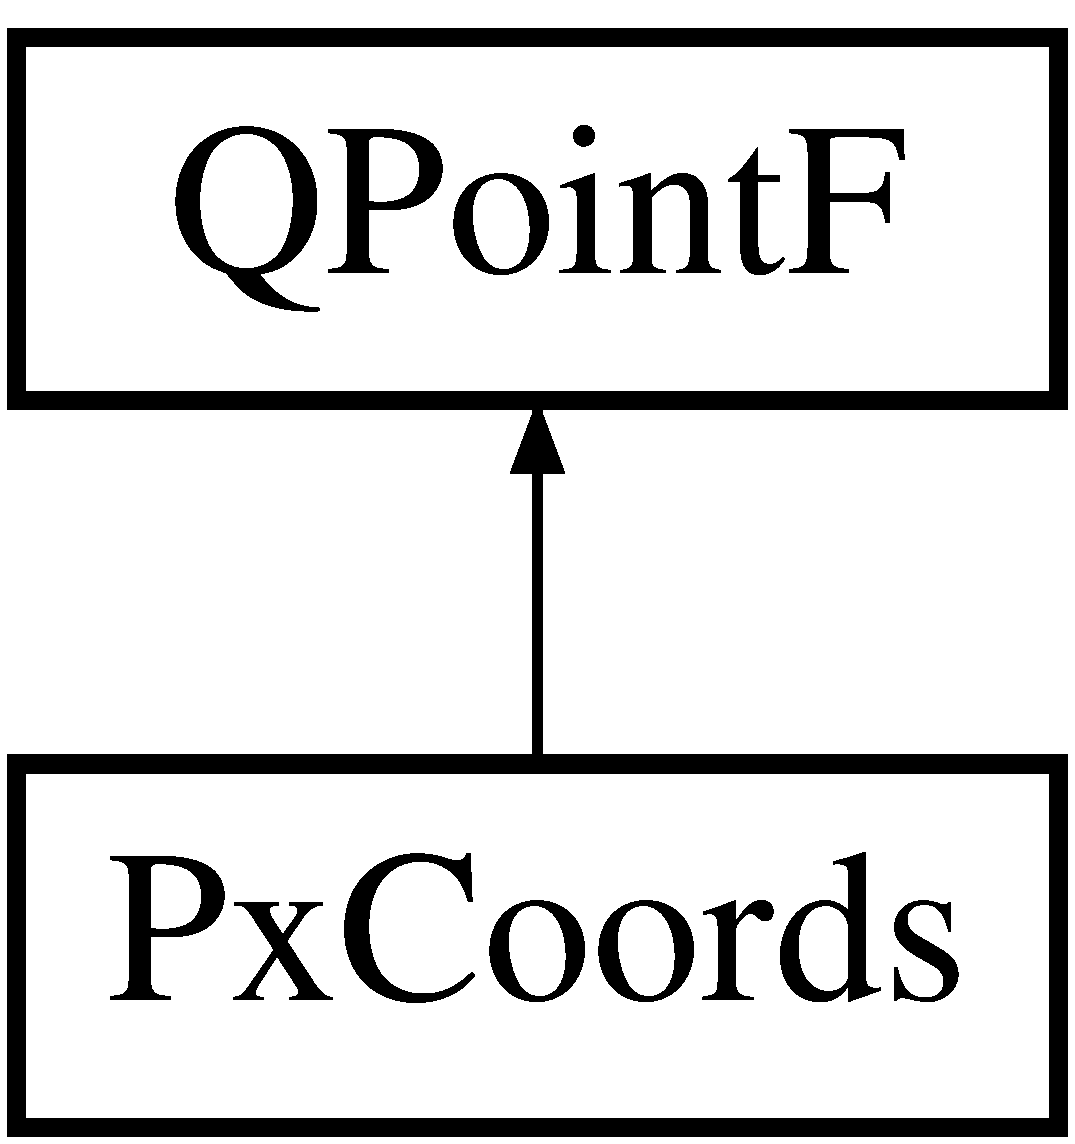
\includegraphics[height=2.000000cm]{class_px_coords}
\end{center}
\end{figure}
\subsection*{Public Member Functions}
\begin{DoxyCompactItemize}
\item 
\hypertarget{class_px_coords_af7f17b5bb6fa3261162b4fb5df854236}{}\label{class_px_coords_af7f17b5bb6fa3261162b4fb5df854236} 
{\bfseries Px\+Coords} (qreal x, qreal y)
\item 
\hypertarget{class_px_coords_a589dea0fc7f89609399528ce47788b74}{}\label{class_px_coords_a589dea0fc7f89609399528ce47788b74} 
{\bfseries Px\+Coords} (const Q\+PointF \&p)
\item 
\hypertarget{class_px_coords_ad38e146a7d9908ac31ddae47a1b765ff}{}\label{class_px_coords_ad38e146a7d9908ac31ddae47a1b765ff} 
{\bfseries Px\+Coords} (const Q\+Point \&p)
\item 
\hypertarget{class_px_coords_a258b2927d40dc866bfbdd0d02a0afa31}{}\label{class_px_coords_a258b2927d40dc866bfbdd0d02a0afa31} 
{\bfseries Px\+Coords} (int x, int y)
\end{DoxyCompactItemize}


\subsection{Detailed Description}
The \hyperlink{class_px_coords}{Px\+Coords} class describe positions with real pixel coordinates. 

Theses coordinates describe the pixel position.

\begin{DoxySeeAlso}{See also}
\hyperlink{class_rl_coords}{Rl\+Coords}, \hyperlink{class_cl_coords}{Cl\+Coords}, \hyperlink{class_pt_coords}{Pt\+Coords} 
\end{DoxySeeAlso}


The documentation for this class was generated from the following file\+:\begin{DoxyCompactItemize}
\item 
src/editor/\+Game/\hyperlink{mappainter_8h}{mappainter.\+h}\end{DoxyCompactItemize}

\hypertarget{class_quiet_combo_box}{\section{\-Quiet\-Combo\-Box \-Class \-Reference}
\label{class_quiet_combo_box}\index{\-Quiet\-Combo\-Box@{\-Quiet\-Combo\-Box}}
}
\subsection*{\-Public \-Slots}
\begin{DoxyCompactItemize}
\item 
\hypertarget{class_quiet_combo_box_a760934024a1d11cba8a51d993fb47dba}{void {\bfseries set\-Model} (\-Q\-Abstract\-Item\-Model $\ast$model)}\label{class_quiet_combo_box_a760934024a1d11cba8a51d993fb47dba}

\item 
\hypertarget{class_quiet_combo_box_a4134cf3f62ef653ee24d8b52cea56455}{void {\bfseries set\-Current\-Index} (int index)}\label{class_quiet_combo_box_a4134cf3f62ef653ee24d8b52cea56455}

\end{DoxyCompactItemize}
\subsection*{\-Signals}
\begin{DoxyCompactItemize}
\item 
\hypertarget{class_quiet_combo_box_a6312d1e75b1dcb4c5c3b6ad1ac4be524}{void {\bfseries user\-Changed\-Current\-Index} (int)}\label{class_quiet_combo_box_a6312d1e75b1dcb4c5c3b6ad1ac4be524}

\end{DoxyCompactItemize}
\subsection*{\-Public \-Member \-Functions}
\begin{DoxyCompactItemize}
\item 
\hypertarget{class_quiet_combo_box_a030bd6a01f30ba67f4b8cf15b959d966}{{\bfseries \-Quiet\-Combo\-Box} (\-Q\-Widget $\ast$parent=nullptr)}\label{class_quiet_combo_box_a030bd6a01f30ba67f4b8cf15b959d966}

\end{DoxyCompactItemize}


\-The documentation for this class was generated from the following files\-:\begin{DoxyCompactItemize}
\item 
src/editor/\-G\-U\-I/quietwidgets.\-h\item 
src/editor/\-G\-U\-I/quietwidgets.\-cpp\end{DoxyCompactItemize}

\hypertarget{class_rl_coords}{}\section{Rl\+Coords Class Reference}
\label{class_rl_coords}\index{Rl\+Coords@{Rl\+Coords}}


The \hyperlink{class_rl_coords}{Rl\+Coords} class describe positions with relative coordinates.  




{\ttfamily \#include $<$mappainter.\+h$>$}

Inheritance diagram for Rl\+Coords\+:\begin{figure}[H]
\begin{center}
\leavevmode
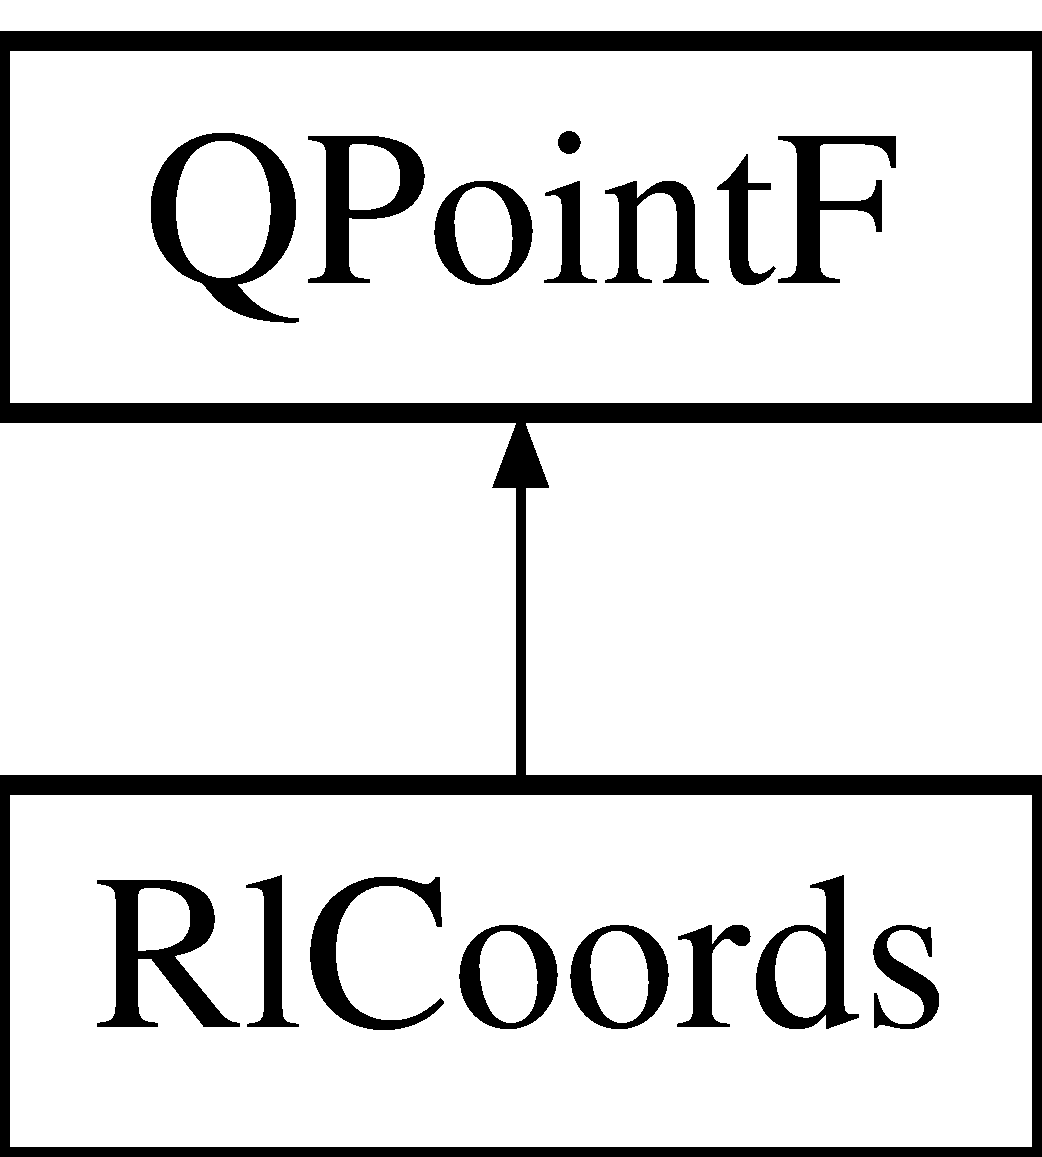
\includegraphics[height=2.000000cm]{class_rl_coords}
\end{center}
\end{figure}
\subsection*{Public Member Functions}
\begin{DoxyCompactItemize}
\item 
\hypertarget{class_rl_coords_ada69216f57050aa6a7b88aa4cb051335}{}\label{class_rl_coords_ada69216f57050aa6a7b88aa4cb051335} 
{\bfseries Rl\+Coords} (qreal x, qreal y)
\item 
\hypertarget{class_rl_coords_a71620c03bf57e61ec3b35af29dab3382}{}\label{class_rl_coords_a71620c03bf57e61ec3b35af29dab3382} 
{\bfseries Rl\+Coords} (const Q\+PointF \&p)
\end{DoxyCompactItemize}


\subsection{Detailed Description}
The \hyperlink{class_rl_coords}{Rl\+Coords} class describe positions with relative coordinates. 

Theses coordinates have values in $[0,1]$, for every point in the view.

\begin{DoxySeeAlso}{See also}
\hyperlink{class_cl_coords}{Cl\+Coords} \hyperlink{class_pt_coords}{Pt\+Coords}, \hyperlink{class_px_coords}{Px\+Coords} 
\end{DoxySeeAlso}


The documentation for this class was generated from the following file\+:\begin{DoxyCompactItemize}
\item 
src/editor/\+Game/\hyperlink{mappainter_8h}{mappainter.\+h}\end{DoxyCompactItemize}

\hypertarget{class_selection_dock}{\section{\-Selection\-Dock \-Class \-Reference}
\label{class_selection_dock}\index{\-Selection\-Dock@{\-Selection\-Dock}}
}


\-The \hyperlink{class_selection_dock}{\-Selection\-Dock} class provides a \hyperlink{class_b_dock_widget}{\-B\-Dock\-Widget} to edit how the \char`\"{}cell\char`\"{} \hyperlink{class_cell}{\-Cell} selection behaves.  




{\ttfamily \#include $<$selectiondock.\-h$>$}

\-Inheritance diagram for \-Selection\-Dock\-:\begin{figure}[H]
\begin{center}
\leavevmode
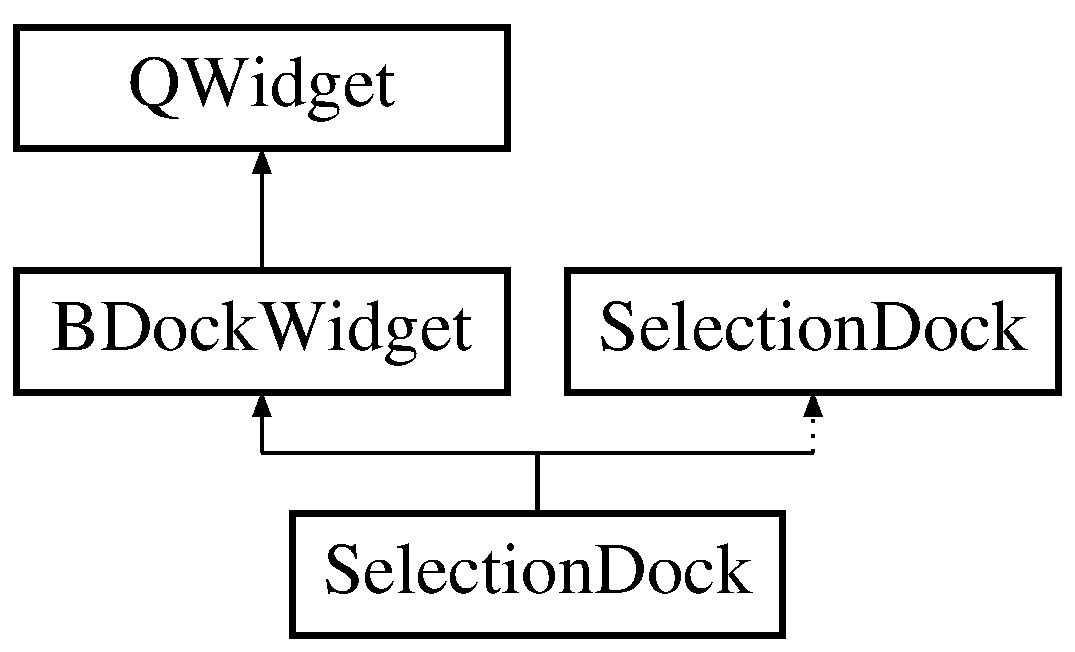
\includegraphics[height=2.000000cm]{class_selection_dock}
\end{center}
\end{figure}
\subsection*{\-Public \-Member \-Functions}
\begin{DoxyCompactItemize}
\item 
\hypertarget{class_selection_dock_a91607ae2abc9aabc3fecfdd10c08571c}{{\bfseries \-Selection\-Dock} (\hyperlink{class_map_viewer}{\-Map\-Viewer} $\ast$mv, \-Q\-Widget $\ast$parent=0)}\label{class_selection_dock_a91607ae2abc9aabc3fecfdd10c08571c}

\end{DoxyCompactItemize}


\subsection{\-Detailed \-Description}
\-The \hyperlink{class_selection_dock}{\-Selection\-Dock} class provides a \hyperlink{class_b_dock_widget}{\-B\-Dock\-Widget} to edit how the \char`\"{}cell\char`\"{} \hyperlink{class_cell}{\-Cell} selection behaves. 

\-The documentation for this class was generated from the following files\-:\begin{DoxyCompactItemize}
\item 
src/editor/\-G\-U\-I/\-Tabs/\-Map\-Tab/\hyperlink{selectiondock_8h}{selectiondock.\-h}\item 
src/editor/\-G\-U\-I/\-Tabs/\-Map\-Tab/selectiondock.\-cpp\end{DoxyCompactItemize}

\hypertarget{class_tab_acces}{\section{\-Tab\-Acces \-Class \-Reference}
\label{class_tab_acces}\index{\-Tab\-Acces@{\-Tab\-Acces}}
}
\subsection*{\-Signals}
\begin{DoxyCompactItemize}
\item 
\hypertarget{class_tab_acces_a3a44992ceb2227664fce84ed26ae226c}{void {\bfseries activated} (int i)}\label{class_tab_acces_a3a44992ceb2227664fce84ed26ae226c}

\end{DoxyCompactItemize}
\subsection*{\-Public \-Member \-Functions}
\begin{DoxyCompactItemize}
\item 
\hypertarget{class_tab_acces_a0e6bcf25a31952e09517ce2273f81786}{{\bfseries \-Tab\-Acces} (int i, const \-Q\-String \&n, const \-Q\-Pixmap \&p, \-Q\-Widget $\ast$parent=0)}\label{class_tab_acces_a0e6bcf25a31952e09517ce2273f81786}

\item 
\hypertarget{class_tab_acces_a2b5298cbcbd0e7e880d7418dea03aa53}{void {\bfseries set\-Active} (bool a)}\label{class_tab_acces_a2b5298cbcbd0e7e880d7418dea03aa53}

\end{DoxyCompactItemize}


\-The documentation for this class was generated from the following files\-:\begin{DoxyCompactItemize}
\item 
src/editor/\-G\-U\-I/tabacces.\-h\item 
src/editor/\-G\-U\-I/tabacces.\-cpp\end{DoxyCompactItemize}

\hypertarget{class_tab_bar}{\section{\-Tab\-Bar \-Class \-Reference}
\label{class_tab_bar}\index{\-Tab\-Bar@{\-Tab\-Bar}}
}
\subsection*{\-Public \-Slots}
\begin{DoxyCompactItemize}
\item 
\hypertarget{class_tab_bar_a71b20e36e9d73a3ab7de30af404b4f67}{void {\bfseries set\-Current\-Tab} (int t)}\label{class_tab_bar_a71b20e36e9d73a3ab7de30af404b4f67}

\end{DoxyCompactItemize}
\subsection*{\-Signals}
\begin{DoxyCompactItemize}
\item 
\hypertarget{class_tab_bar_af1823815958705f27ab8e7a90262c27e}{void {\bfseries current\-Tab\-Changed} (int)}\label{class_tab_bar_af1823815958705f27ab8e7a90262c27e}

\end{DoxyCompactItemize}
\subsection*{\-Public \-Member \-Functions}
\begin{DoxyCompactItemize}
\item 
\hypertarget{class_tab_bar_ad91da41e8bfec9cf184f36b49ba4bf6b}{{\bfseries \-Tab\-Bar} (\-Q\-Widget $\ast$parent=0)}\label{class_tab_bar_ad91da41e8bfec9cf184f36b49ba4bf6b}

\item 
\hypertarget{class_tab_bar_a4eb314982505463c3244a007b4e5a813}{void {\bfseries add\-Tab\-Acces} (const \-Q\-String \&n, const \-Q\-Pixmap \&p, \hyperlink{class_tab_widget}{\-Tab\-Widget} $\ast$w)}\label{class_tab_bar_a4eb314982505463c3244a007b4e5a813}

\item 
\hypertarget{class_tab_bar_a78cf61eaaaf5ceed7de52bc3ff1ca07c}{int {\bfseries current\-Tab} () const }\label{class_tab_bar_a78cf61eaaaf5ceed7de52bc3ff1ca07c}

\item 
\hypertarget{class_tab_bar_a6bb891b77ab937e8d97022cf7d46cf3a}{void {\bfseries set\-Tabs\-Enabled} (bool e)}\label{class_tab_bar_a6bb891b77ab937e8d97022cf7d46cf3a}

\end{DoxyCompactItemize}


\-The documentation for this class was generated from the following files\-:\begin{DoxyCompactItemize}
\item 
src/editor/\-G\-U\-I/tabbar.\-h\item 
src/editor/\-G\-U\-I/tabbar.\-cpp\end{DoxyCompactItemize}

\hypertarget{class_tab_widget}{\section{\-Tab\-Widget \-Class \-Reference}
\label{class_tab_widget}\index{\-Tab\-Widget@{\-Tab\-Widget}}
}
\-Inheritance diagram for \-Tab\-Widget\-:\begin{figure}[H]
\begin{center}
\leavevmode
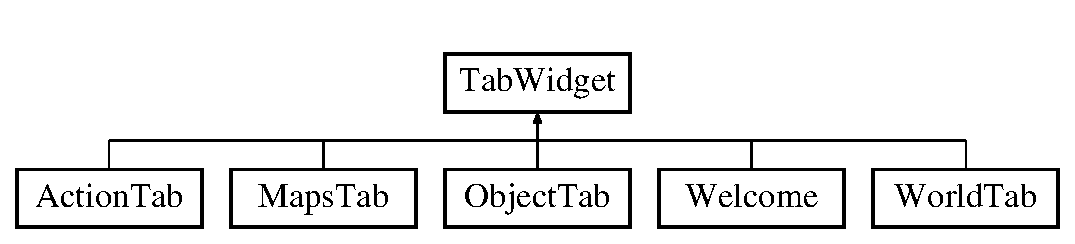
\includegraphics[height=2.000000cm]{class_tab_widget}
\end{center}
\end{figure}
\subsection*{\-Public \-Member \-Functions}
\begin{DoxyCompactItemize}
\item 
\hypertarget{class_tab_widget_a5aad386a078e6085d72e5ade6c4a678d}{{\bfseries \-Tab\-Widget} (\-Q\-Widget $\ast$parent=0)}\label{class_tab_widget_a5aad386a078e6085d72e5ade6c4a678d}

\item 
\hypertarget{class_tab_widget_a98e3d1229d031db9584aee4e32f704ba}{int {\bfseries index} () const }\label{class_tab_widget_a98e3d1229d031db9584aee4e32f704ba}

\item 
\hypertarget{class_tab_widget_a39b94d30a678d6e9c93669888bfb8de3}{void {\bfseries set\-Index} (int i)}\label{class_tab_widget_a39b94d30a678d6e9c93669888bfb8de3}

\item 
\hypertarget{class_tab_widget_a2272e79554d0cb0aa69da95d7b4cc0b3}{virtual void {\bfseries update\-Game} ()}\label{class_tab_widget_a2272e79554d0cb0aa69da95d7b4cc0b3}

\end{DoxyCompactItemize}


\-The documentation for this class was generated from the following files\-:\begin{DoxyCompactItemize}
\item 
src/editor/\-G\-U\-I/\-Tabs/tabwidget.\-h\item 
src/editor/\-G\-U\-I/\-Tabs/tabwidget.\-cpp\end{DoxyCompactItemize}

\hypertarget{class_type}{\section{\-Type$<$ \-T $>$ \-Class \-Template \-Reference}
\label{class_type}\index{\-Type$<$ T $>$@{\-Type$<$ T $>$}}
}


\-The \hyperlink{class_type}{\-Type} class represent a type of object.  




{\ttfamily \#include $<$typedobject.\-hxx$>$}

\-Inheritance diagram for \-Type$<$ \-T $>$\-:\begin{figure}[H]
\begin{center}
\leavevmode
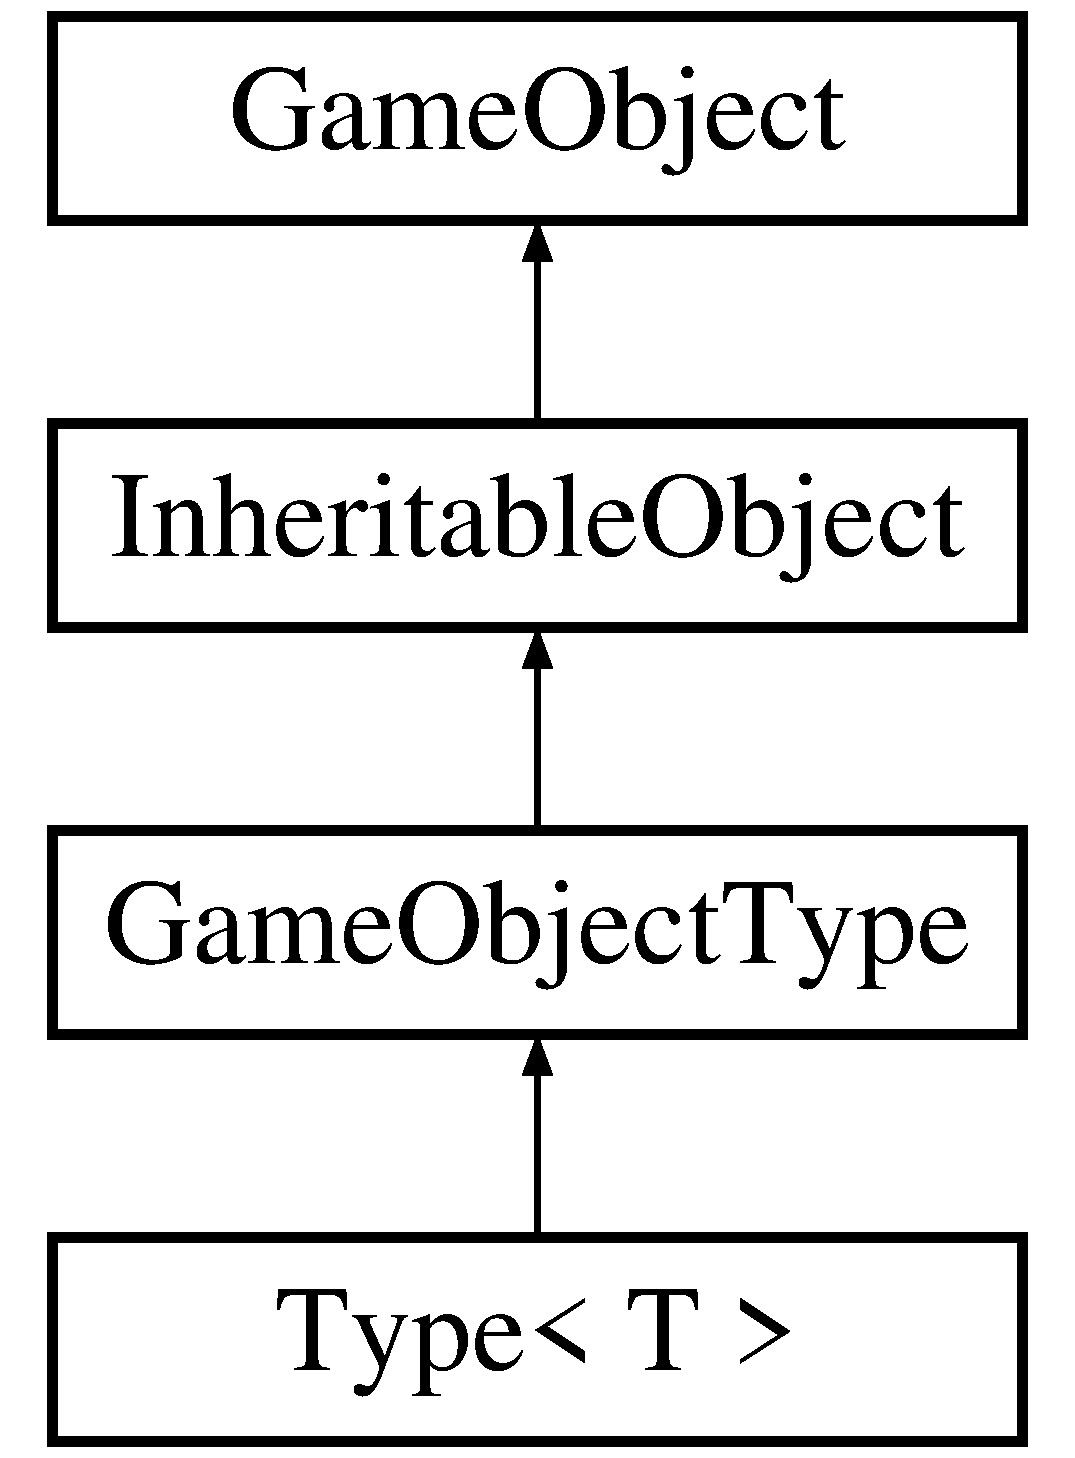
\includegraphics[height=4.000000cm]{class_type}
\end{center}
\end{figure}
\subsection*{\-Public \-Member \-Functions}
\begin{DoxyCompactItemize}
\item 
\hypertarget{class_type_aea9c6be9b52e1e356ffb0123f2815c21}{{\bfseries \-Type} (\hyperlink{class_default_types}{\-Default\-Types} \&\hyperlink{class_game_object_af3deaf39cde23c189765634e32e95bb4}{parent})}\label{class_type_aea9c6be9b52e1e356ffb0123f2815c21}

\item 
\hypertarget{class_type_a8d71537af478aaedd7aaab6b50e5bfb9}{{\bfseries \-Type} (\-T \&\hyperlink{class_inheritable_object_ac87a3c55ca4be252c527a29fe162bb15}{ancestor})}\label{class_type_a8d71537af478aaedd7aaab6b50e5bfb9}

\end{DoxyCompactItemize}


\subsection{\-Detailed \-Description}
\subsubsection*{template$<$class \-T$>$class Type$<$ T $>$}

\-The \hyperlink{class_type}{\-Type} class represent a type of object. 

\-It adds to \hyperlink{class_game_object_type}{\-Game\-Object\-Type} a constrain on the objects that can be used as type, defined by le {\ttfamily class} {\ttfamily \-T} template argument.

\begin{DoxyNote}{\-Note}
\-The {\ttfamily class} {\ttfamily \-T} template argument has to be inherited from \hyperlink{class_type}{\-Type}. (the application won't compile otherwise)
\end{DoxyNote}
\begin{DoxySeeAlso}{\-See also}
\hyperlink{class_cell_type}{\-Cell\-Type}, \hyperlink{class_object_type}{\-Object\-Type} 
\end{DoxySeeAlso}


\-The documentation for this class was generated from the following file\-:\begin{DoxyCompactItemize}
\item 
src/editor/\-Game/\hyperlink{typedobject_8hxx}{typedobject.\-hxx}\end{DoxyCompactItemize}

\hypertarget{class_typed_object}{\section{\-Typed\-Object$<$ \-T $>$ \-Class \-Template \-Reference}
\label{class_typed_object}\index{\-Typed\-Object$<$ T $>$@{\-Typed\-Object$<$ T $>$}}
}


\-The \hyperlink{class_typed_object}{\-Typed\-Object} class is the base class for \hyperlink{class_game_object}{\-Game\-Object} with a mutable \hyperlink{class_type}{\-Type}.  




{\ttfamily \#include $<$typedobject.\-hxx$>$}

\-Inheritance diagram for \-Typed\-Object$<$ \-T $>$\-:\begin{figure}[H]
\begin{center}
\leavevmode
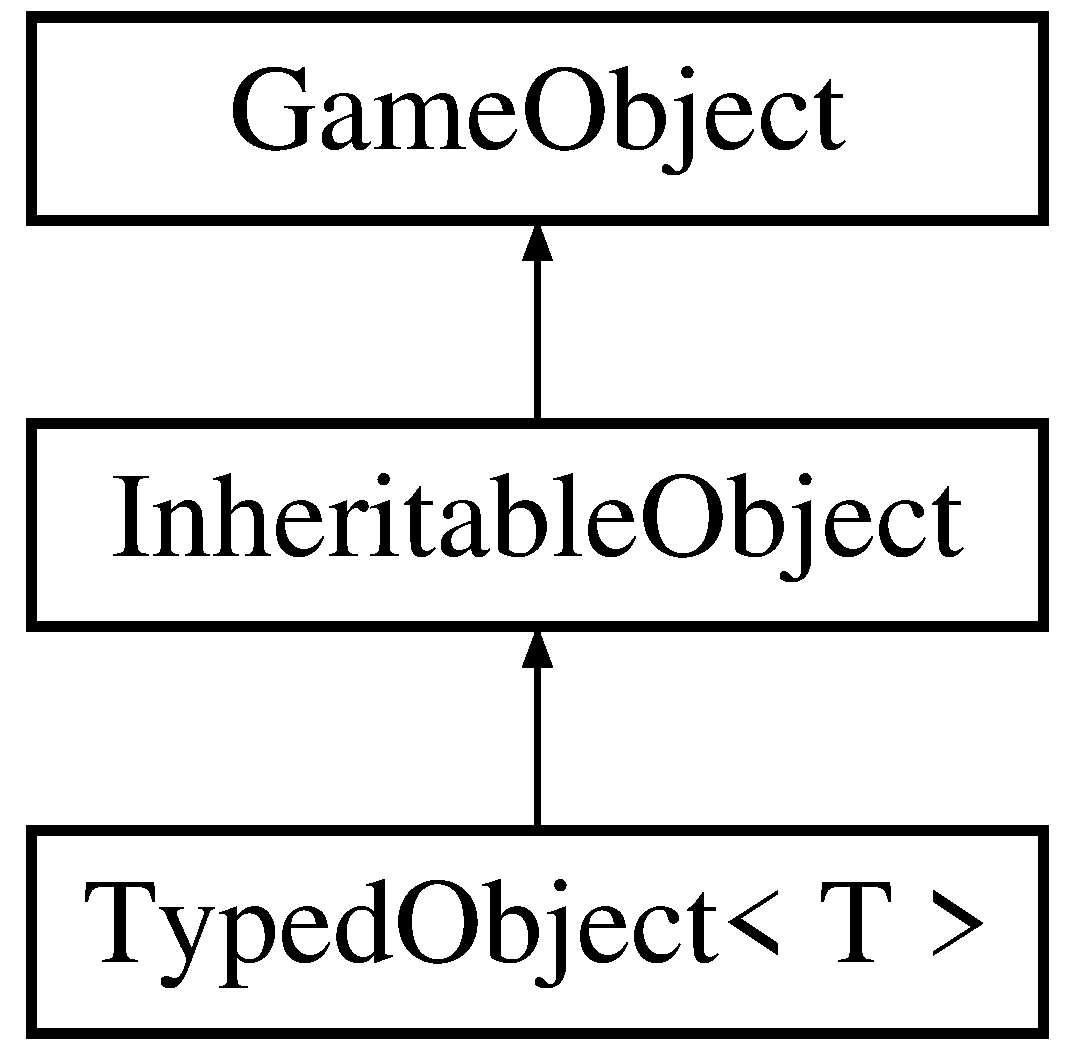
\includegraphics[height=3.000000cm]{class_typed_object}
\end{center}
\end{figure}
\subsection*{\-Public \-Member \-Functions}
\begin{DoxyCompactItemize}
\item 
\hypertarget{class_typed_object_a10319b334d59e8c51a05f56b37001381}{{\bfseries \-Typed\-Object} (\-T \&type, \hyperlink{class_game_object}{\-Game\-Object} \&\hyperlink{class_game_object_af3deaf39cde23c189765634e32e95bb4}{parent})}\label{class_typed_object_a10319b334d59e8c51a05f56b37001381}

\item 
\hypertarget{class_typed_object_af7e793c302dad222271aaad3f800b81d}{\-T \& {\bfseries object\-Type} ()}\label{class_typed_object_af7e793c302dad222271aaad3f800b81d}

\item 
\hypertarget{class_typed_object_a0ece67a4e69c1cb1c127e2316236f8a3}{void {\bfseries set\-Object\-Type} (\-T \&type)}\label{class_typed_object_a0ece67a4e69c1cb1c127e2316236f8a3}

\end{DoxyCompactItemize}
\subsection*{\-Protected \-Attributes}
\begin{DoxyCompactItemize}
\item 
\hypertarget{class_typed_object_aa069c8f9698828c4b5775782cc369de5}{\-T $\ast$ {\bfseries a\-Object\-Type}}\label{class_typed_object_aa069c8f9698828c4b5775782cc369de5}

\end{DoxyCompactItemize}


\subsection{\-Detailed \-Description}
\subsubsection*{template$<$class \-T$>$class Typed\-Object$<$ T $>$}

\-The \hyperlink{class_typed_object}{\-Typed\-Object} class is the base class for \hyperlink{class_game_object}{\-Game\-Object} with a mutable \hyperlink{class_type}{\-Type}. 

\-It adds to \hyperlink{class_inheritable_object}{\-Inheritable\-Object} the guarranty that the object has a type, with a constrain on it defined by le {\ttfamily class} {\ttfamily \-T} template argument.

\begin{DoxyNote}{\-Note}
\-The {\ttfamily class} {\ttfamily \-T} template argument has to be inherited from \hyperlink{class_type}{\-Type}. (the application won't compile otherwise)
\end{DoxyNote}
\begin{DoxySeeAlso}{\-See also}
\hyperlink{class_cell}{\-Cell}, \hyperlink{class_object}{\-Object} 
\end{DoxySeeAlso}


\-The documentation for this class was generated from the following file\-:\begin{DoxyCompactItemize}
\item 
src/editor/\-Game/\hyperlink{typedobject_8hxx}{typedobject.\-hxx}\end{DoxyCompactItemize}

\hypertarget{class_type_item_model}{\section{\-Type\-Item\-Model \-Class \-Reference}
\label{class_type_item_model}\index{\-Type\-Item\-Model@{\-Type\-Item\-Model}}
}


\-The \hyperlink{class_type_item_model}{\-Type\-Item\-Model} class presents the type hierarchy using the \-Q\-Abstract\-Item\-Model interface.  




{\ttfamily \#include $<$typeitemmodel.\-h$>$}

\subsection*{\-Public \-Member \-Functions}
\begin{DoxyCompactItemize}
\item 
\hypertarget{class_type_item_model_a108cfb2528711b687b9b0c15880b766d}{{\bfseries \-Type\-Item\-Model} (\-Q\-Object $\ast$parent=nullptr)}\label{class_type_item_model_a108cfb2528711b687b9b0c15880b766d}

\item 
\hypertarget{class_type_item_model_a57cef0a628dafeef516a81233e7010b3}{int {\bfseries column\-Count} (const \-Q\-Model\-Index \&parent) const }\label{class_type_item_model_a57cef0a628dafeef516a81233e7010b3}

\item 
\hypertarget{class_type_item_model_a689148d85b1586617c3125a9c4ef5f13}{int {\bfseries row\-Count} (const \-Q\-Model\-Index \&parent) const }\label{class_type_item_model_a689148d85b1586617c3125a9c4ef5f13}

\item 
\hypertarget{class_type_item_model_a01a5d3115ec4282ea6ac98ceafd4b386}{\-Qt\-::\-Item\-Flags {\bfseries flags} (const \-Q\-Model\-Index \&index) const }\label{class_type_item_model_a01a5d3115ec4282ea6ac98ceafd4b386}

\item 
\hypertarget{class_type_item_model_a2d1957a8b511de7f6c324e92cec767ac}{\-Q\-Variant {\bfseries data} (const \-Q\-Model\-Index \&index, int role) const }\label{class_type_item_model_a2d1957a8b511de7f6c324e92cec767ac}

\item 
\hypertarget{class_type_item_model_a86a11d88b6fde64923f683033478f15e}{\-Q\-Model\-Index {\bfseries index} (int row, int column, const \-Q\-Model\-Index \&parent) const }\label{class_type_item_model_a86a11d88b6fde64923f683033478f15e}

\item 
\hypertarget{class_type_item_model_aa5ba32873ce3479effa833fcb88e12af}{\-Q\-Model\-Index {\bfseries parent} (const \-Q\-Model\-Index \&child) const }\label{class_type_item_model_aa5ba32873ce3479effa833fcb88e12af}

\item 
\hypertarget{class_type_item_model_a58745f2062586349fc312afb792cc85e}{\-Q\-Variant {\bfseries header\-Data} (int section, \-Qt\-::\-Orientation orientation, int role) const }\label{class_type_item_model_a58745f2062586349fc312afb792cc85e}

\item 
\hypertarget{class_type_item_model_a652f8f9324f96faa3a0ba0118d157a6e}{bool {\bfseries set\-Data} (const \-Q\-Model\-Index \&index, const \-Q\-Variant \&value, int role)}\label{class_type_item_model_a652f8f9324f96faa3a0ba0118d157a6e}

\item 
\hypertarget{class_type_item_model_a6a52d9f08010bf7535a6280ce5bf6ba4}{void {\bfseries set\-Game} (\hyperlink{class_game}{\-Game} $\ast$g)}\label{class_type_item_model_a6a52d9f08010bf7535a6280ce5bf6ba4}

\end{DoxyCompactItemize}


\subsection{\-Detailed \-Description}
\-The \hyperlink{class_type_item_model}{\-Type\-Item\-Model} class presents the type hierarchy using the \-Q\-Abstract\-Item\-Model interface. 

\begin{DoxySeeAlso}{\-See also}
\hyperlink{class_type_tree_item}{\-Type\-Tree\-Item} 
\end{DoxySeeAlso}


\-The documentation for this class was generated from the following files\-:\begin{DoxyCompactItemize}
\item 
src/editor/\-Game/\-Item\-Models/\hyperlink{typeitemmodel_8h}{typeitemmodel.\-h}\item 
src/editor/\-Game/\-Item\-Models/typeitemmodel.\-cpp\end{DoxyCompactItemize}

\hypertarget{class_type_tree_item}{\section{\-Type\-Tree\-Item \-Class \-Reference}
\label{class_type_tree_item}\index{\-Type\-Tree\-Item@{\-Type\-Tree\-Item}}
}


\-The \hyperlink{class_type_tree_item}{\-Type\-Tree\-Item} class defines an tree item for the \-Type\-Item\-Model class.  




{\ttfamily \#include $<$typeitemmodel.\-h$>$}

\subsection*{\-Public \-Member \-Functions}
\begin{DoxyCompactItemize}
\item 
\hypertarget{class_type_tree_item_a0955484034ad18bc778655fbcf78b435}{{\bfseries \-Type\-Tree\-Item} (\hyperlink{class_game}{\-Game} $\ast$game)}\label{class_type_tree_item_a0955484034ad18bc778655fbcf78b435}

\item 
\hypertarget{class_type_tree_item_a160ac83e2f8d1161735363bbb72ab0bb}{\-Qt\-::\-Item\-Flags {\bfseries flags} (int col) const }\label{class_type_tree_item_a160ac83e2f8d1161735363bbb72ab0bb}

\item 
\hypertarget{class_type_tree_item_a8665b9f195b39093ca6116ff65b09412}{\-Q\-Variant {\bfseries data} (int col, int role) const }\label{class_type_tree_item_a8665b9f195b39093ca6116ff65b09412}

\item 
\hypertarget{class_type_tree_item_a86e9e8d9fca786ac45e81e78d01b9397}{\hyperlink{class_type_tree_item}{\-Type\-Tree\-Item} $\ast$ {\bfseries parent} () const }\label{class_type_tree_item_a86e9e8d9fca786ac45e81e78d01b9397}

\item 
\hypertarget{class_type_tree_item_a06d4681904a79553a81b09d4b31f0731}{\hyperlink{class_type_tree_item}{\-Type\-Tree\-Item} $\ast$ {\bfseries child} (int row) const }\label{class_type_tree_item_a06d4681904a79553a81b09d4b31f0731}

\item 
\hypertarget{class_type_tree_item_a5308dd7d3672750f2d862683d2387dcc}{int {\bfseries row\-Count} () const }\label{class_type_tree_item_a5308dd7d3672750f2d862683d2387dcc}

\item 
\hypertarget{class_type_tree_item_aed3d1b02b89bc0a22842bc54833eaecd}{int {\bfseries row} () const }\label{class_type_tree_item_aed3d1b02b89bc0a22842bc54833eaecd}

\item 
\hypertarget{class_type_tree_item_a465d8935d2564e05d16a2765b8b69434}{bool {\bfseries set\-Data} (int col, \-Q\-Variant value, int role)}\label{class_type_tree_item_a465d8935d2564e05d16a2765b8b69434}

\end{DoxyCompactItemize}


\subsection{\-Detailed \-Description}
\-The \hyperlink{class_type_tree_item}{\-Type\-Tree\-Item} class defines an tree item for the \-Type\-Item\-Model class. 

\-It ensures items to have a parent, and provides abstract item (not related to \hyperlink{class_type}{\-Type} object). 

\-The documentation for this class was generated from the following files\-:\begin{DoxyCompactItemize}
\item 
src/editor/\-Game/\-Item\-Models/\hyperlink{typeitemmodel_8h}{typeitemmodel.\-h}\item 
src/editor/\-Game/\-Item\-Models/typeitemmodel.\-cpp\end{DoxyCompactItemize}

\hypertarget{class_welcome}{\section{\-Welcome \-Class \-Reference}
\label{class_welcome}\index{\-Welcome@{\-Welcome}}
}
\-Inheritance diagram for \-Welcome\-:\begin{figure}[H]
\begin{center}
\leavevmode
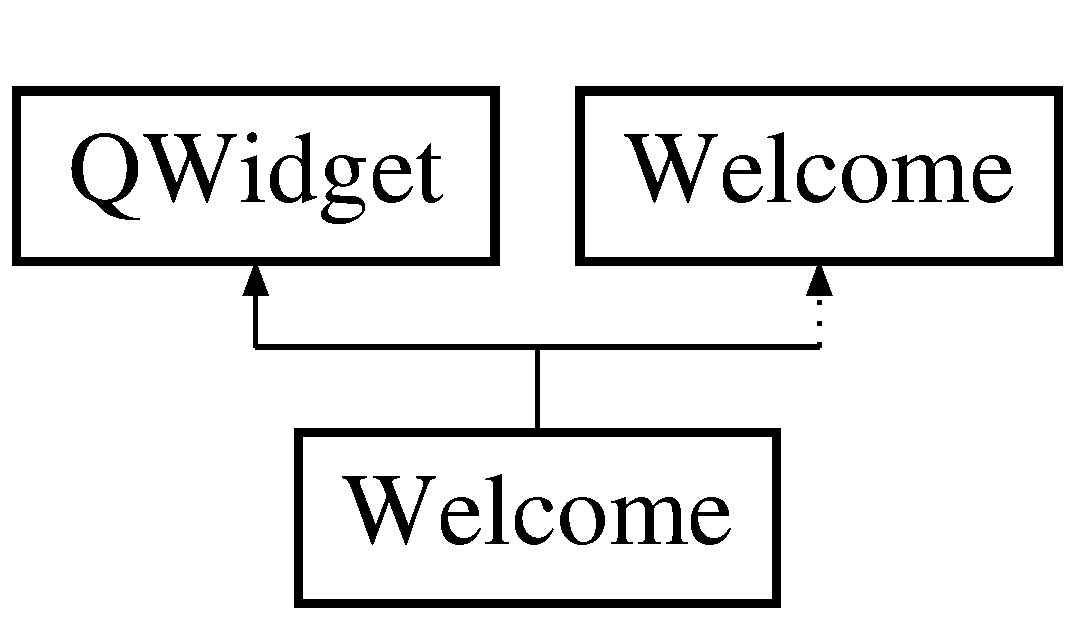
\includegraphics[height=2.000000cm]{class_welcome}
\end{center}
\end{figure}
\subsection*{\-Public \-Member \-Functions}
\begin{DoxyCompactItemize}
\item 
\hypertarget{class_welcome_acf62624f1107ddc68761d25febbf10ad}{{\bfseries \-Welcome} (\-Q\-Widget $\ast$parent=0)}\label{class_welcome_acf62624f1107ddc68761d25febbf10ad}

\end{DoxyCompactItemize}


\-The documentation for this class was generated from the following files\-:\begin{DoxyCompactItemize}
\item 
src/editor/\-G\-U\-I/\-Tabs/welcome.\-h\item 
src/editor/\-G\-U\-I/\-Tabs/welcome.\-cpp\end{DoxyCompactItemize}

\hypertarget{class_world}{\section{\-World \-Class \-Reference}
\label{class_world}\index{\-World@{\-World}}
}


\-The \hyperlink{class_world}{\-World} class.  




{\ttfamily \#include $<$game.\-h$>$}

\-Inheritance diagram for \-World\-:\begin{figure}[H]
\begin{center}
\leavevmode
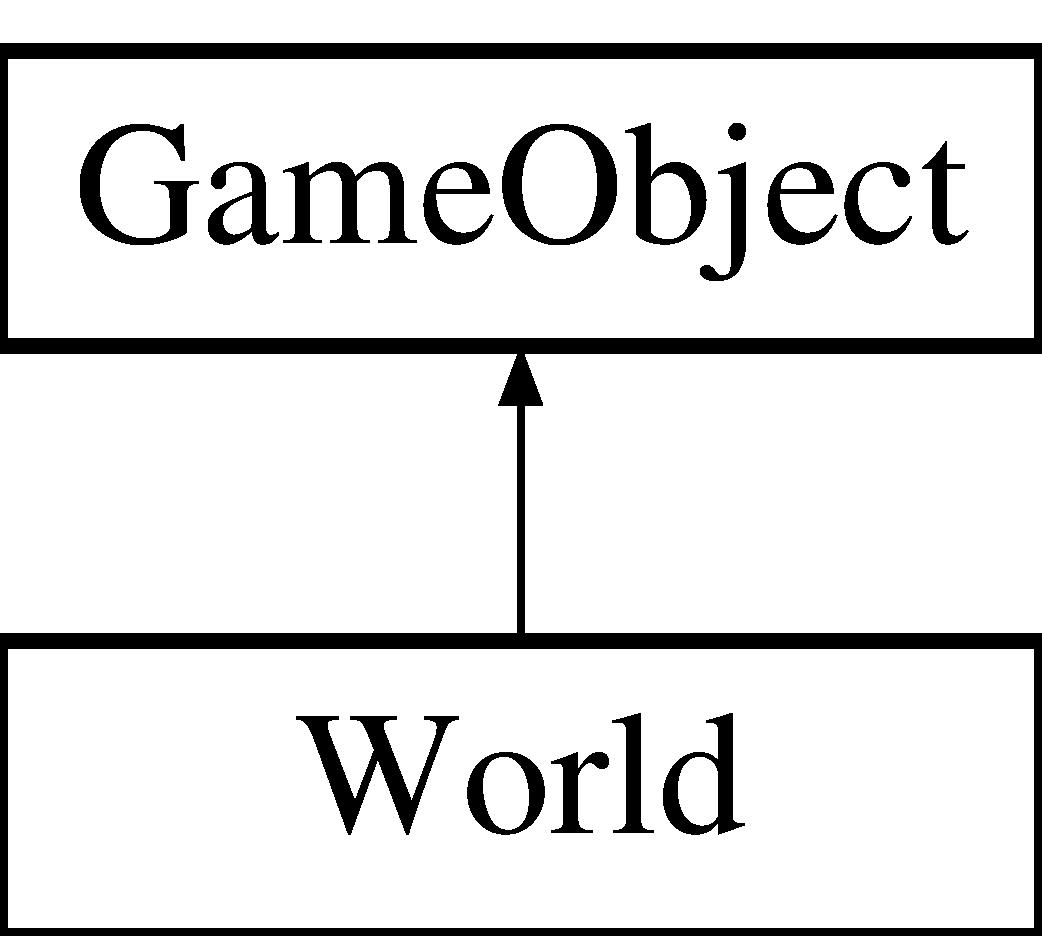
\includegraphics[height=2.000000cm]{class_world}
\end{center}
\end{figure}
\subsection*{\-Public \-Member \-Functions}
\begin{DoxyCompactItemize}
\item 
\hypertarget{class_world_aaf77452519079d4370a5f36d5a511006}{\hyperlink{class_world}{\-World} {\bfseries \-World} (\hyperlink{class_game}{\-Game} $\ast$g, \hyperlink{class_game_object}{\-Game\-Object} $\ast$a\-Parent)}\label{class_world_aaf77452519079d4370a5f36d5a511006}

\item 
\hypertarget{class_world_a842b58f52880ec120cc2cc77383f1711}{\hyperlink{class_default_types}{\-Default\-Types} \& {\bfseries types} ()}\label{class_world_a842b58f52880ec120cc2cc77383f1711}

\item 
\hypertarget{class_world_a7cae44942baff3777efcd62c313f8cfb}{\hyperlink{class_game_object_inventory}{\-Game\-Object\-Inventory} \& {\bfseries objects} ()}\label{class_world_a7cae44942baff3777efcd62c313f8cfb}

\end{DoxyCompactItemize}


\subsection{\-Detailed \-Description}
\-The \hyperlink{class_world}{\-World} class. 

\-The documentation for this class was generated from the following files\-:\begin{DoxyCompactItemize}
\item 
src/editor/\-Game/\hyperlink{game_8h}{game.\-h}\item 
src/editor/\-Game/game.\-cpp\end{DoxyCompactItemize}

\hypertarget{class_world_tab}{\section{\-World\-Tab \-Class \-Reference}
\label{class_world_tab}\index{\-World\-Tab@{\-World\-Tab}}
}


\-The \hyperlink{class_world_tab}{\-World\-Tab} class is the \hyperlink{class_tab_widget}{\-Tab\-Widget} that provides world edition features.  




{\ttfamily \#include $<$worldtab.\-h$>$}

\-Inheritance diagram for \-World\-Tab\-:\begin{figure}[H]
\begin{center}
\leavevmode
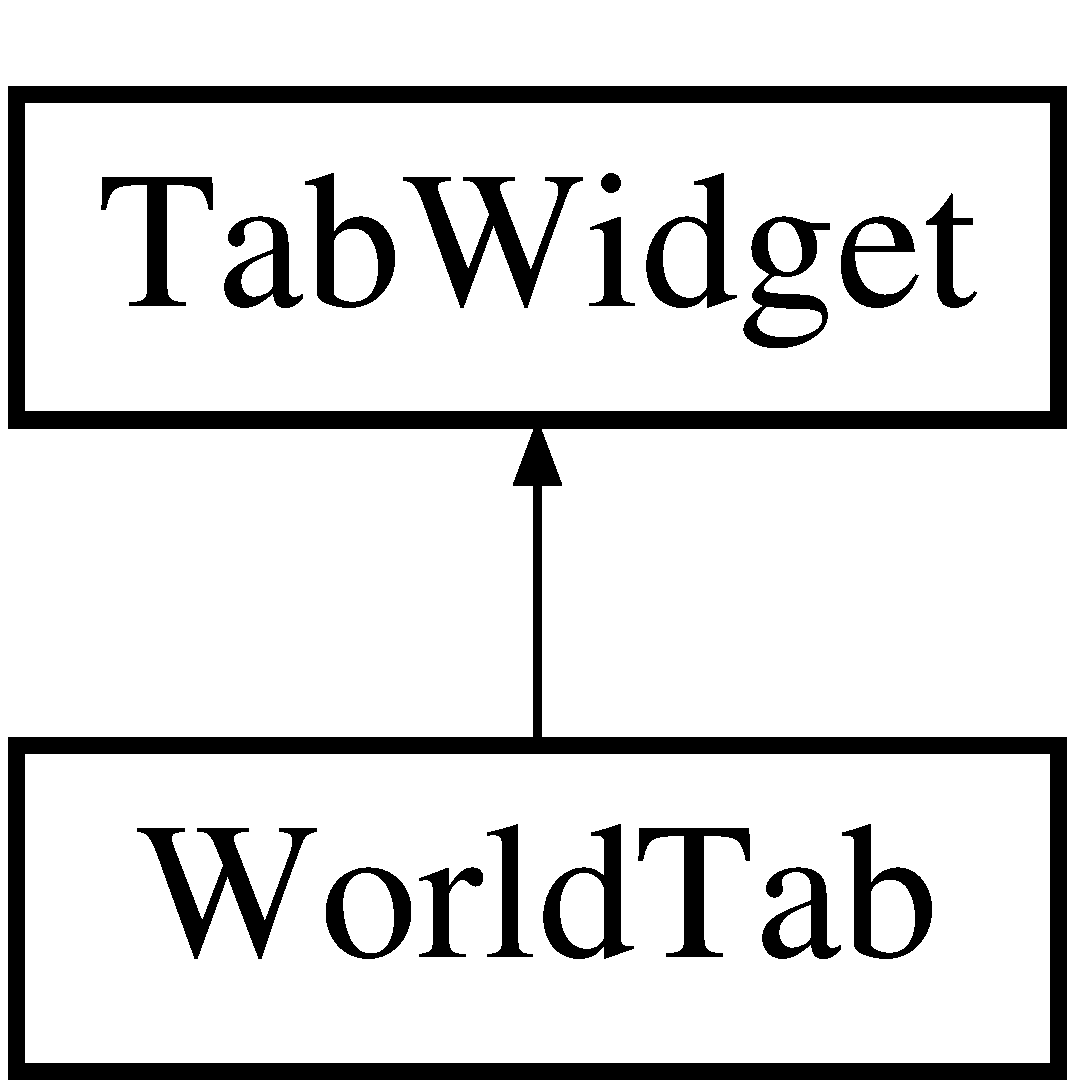
\includegraphics[height=2.000000cm]{class_world_tab}
\end{center}
\end{figure}
\subsection*{\-Signals}
\begin{DoxyCompactItemize}
\item 
\hypertarget{class_world_tab_a57d3f7150343d03ef60502ebccecd622}{void {\bfseries edit\-Map} ()}\label{class_world_tab_a57d3f7150343d03ef60502ebccecd622}

\end{DoxyCompactItemize}
\subsection*{\-Public \-Member \-Functions}
\begin{DoxyCompactItemize}
\item 
\hypertarget{class_world_tab_a8ad97800dd89af4ee32f97823b67ca8e}{{\bfseries \-World\-Tab} (\-Q\-Widget $\ast$parent=0)}\label{class_world_tab_a8ad97800dd89af4ee32f97823b67ca8e}

\item 
\hypertarget{class_world_tab_ae37b09116218cfcc9b1f184eb88a59ee}{void {\bfseries set\-Game} (\hyperlink{class_game}{\-Game} $\ast$g)}\label{class_world_tab_ae37b09116218cfcc9b1f184eb88a59ee}

\end{DoxyCompactItemize}


\subsection{\-Detailed \-Description}
\-The \hyperlink{class_world_tab}{\-World\-Tab} class is the \hyperlink{class_tab_widget}{\-Tab\-Widget} that provides world edition features. 

\-The documentation for this class was generated from the following files\-:\begin{DoxyCompactItemize}
\item 
src/editor/\-G\-U\-I/\-Tabs/\hyperlink{worldtab_8h}{worldtab.\-h}\item 
src/editor/\-G\-U\-I/\-Tabs/worldtab.\-cpp\end{DoxyCompactItemize}

\hypertarget{class_xml_handler}{\section{\-Xml\-Handler \-Class \-Reference}
\label{class_xml_handler}\index{\-Xml\-Handler@{\-Xml\-Handler}}
}
\subsection*{\-Public \-Member \-Functions}
\begin{DoxyCompactItemize}
\item 
\hypertarget{class_xml_handler_a98cf939ef528aa336c7e4b2ae7f1a431}{{\bfseries \-Xml\-Handler} (\hyperlink{class_game}{\-Game} $\ast$g)}\label{class_xml_handler_a98cf939ef528aa336c7e4b2ae7f1a431}

\item 
\hypertarget{class_xml_handler_a23b06b0d562fa3be82b42f46148a4175}{bool {\bfseries start\-Element} (const \-Q\-String \&, const \-Q\-String \&local\-Name, const \-Q\-String \&, const \-Q\-Xml\-Attributes \&atts)}\label{class_xml_handler_a23b06b0d562fa3be82b42f46148a4175}

\item 
\hypertarget{class_xml_handler_a647d0b062e0d8c8d4b65bfe040dee441}{bool {\bfseries end\-Element} (const \-Q\-String \&, const \-Q\-String \&local\-Name, const \-Q\-String \&)}\label{class_xml_handler_a647d0b062e0d8c8d4b65bfe040dee441}

\end{DoxyCompactItemize}


\-The documentation for this class was generated from the following files\-:\begin{DoxyCompactItemize}
\item 
src/editor/\-Game/xmlhandler.\-h\item 
src/editor/\-Game/xmlhandler.\-cpp\end{DoxyCompactItemize}

\chapter{\-File \-Documentation}
\hypertarget{game_8h}{\section{src/editor/\-Game/game.h \-File \-Reference}
\label{game_8h}\index{src/editor/\-Game/game.\-h@{src/editor/\-Game/game.\-h}}
}


\-Definition of the \hyperlink{class_game}{\-Game} and \hyperlink{class_world}{\-World} classes.  


{\ttfamily \#include \char`\"{}object.\-h\char`\"{}}\*
{\ttfamily \#include \char`\"{}map.\-h\char`\"{}}\*
\subsection*{\-Classes}
\begin{DoxyCompactItemize}
\item 
class \hyperlink{class_world}{\-World}
\begin{DoxyCompactList}\small\item\em \-The \hyperlink{class_world}{\-World} class. \end{DoxyCompactList}\item 
class \hyperlink{class_game}{\-Game}
\begin{DoxyCompactList}\small\item\em \-The \hyperlink{class_game}{\-Game} class gather the differents parts needed to describe a game. \end{DoxyCompactList}\end{DoxyCompactItemize}


\subsection{\-Detailed \-Description}
\-Definition of the \hyperlink{class_game}{\-Game} and \hyperlink{class_world}{\-World} classes. 
\hypertarget{gameobject_8h}{\section{src/editor/\-Game/gameobject.h \-File \-Reference}
\label{gameobject_8h}\index{src/editor/\-Game/gameobject.\-h@{src/editor/\-Game/gameobject.\-h}}
}


\-Definition of the base class of the game internal model.  


{\ttfamily \#include $<$\-Qt\-Gui$>$}\*
{\ttfamily \#include $<$assert.\-h$>$}\*
{\ttfamily \#include $<$algorithm$>$}\*
\subsection*{\-Data \-Structures}
\begin{DoxyCompactItemize}
\item 
class \hyperlink{class_parameter}{\-Parameter}
\begin{DoxyCompactList}\small\item\em \-The \hyperlink{class_parameter}{\-Parameter} class represents a parameter with a valid domain of value. \end{DoxyCompactList}\item 
class \hyperlink{class_game_object}{\-Game\-Object}
\begin{DoxyCompactList}\small\item\em \-The \hyperlink{class_game_object}{\-Game\-Object} class is the base class for every part of games. \end{DoxyCompactList}\item 
class \hyperlink{class_inheritable_object}{\-Inheritable\-Object}
\begin{DoxyCompactList}\small\item\em \-The \hyperlink{class_inheritable_object}{\-Inheritable\-Object} class is the base class for every objects that can inherit attributes from an other \hyperlink{class_inheritable_object}{\-Inheritable\-Object}. \end{DoxyCompactList}\item 
class \hyperlink{class_game_object_type}{\-Game\-Object\-Type}
\end{DoxyCompactItemize}
\subsection*{\-Defines}
\begin{DoxyCompactItemize}
\item 
\hypertarget{gameobject_8h_ab330159c4bbdc7d8e10cd05da86565aa}{\#define {\bfseries \-U\-N\-U\-S\-E\-D}(p)}\label{gameobject_8h_ab330159c4bbdc7d8e10cd05da86565aa}

\item 
\hypertarget{gameobject_8h_a9c09ffbe0bea5710ddb0f2bba0c605ae}{\#define {\bfseries \-Type\-Name}(\hyperlink{class_type}{\-Type})~virtual \-Q\-String type\-Name() const\{return \-Q\-Object\-::tr(\#\hyperlink{class_type}{\-Type});\}}\label{gameobject_8h_a9c09ffbe0bea5710ddb0f2bba0c605ae}

\item 
\hypertarget{gameobject_8h_aa4e4db36d846a9d6dff95def8d7507c3}{\#define {\bfseries \-Object\-List\-Def}(\-Objects, \hyperlink{class_type}{\-Type})~private\-: \-Q\-Map$<$int, \hyperlink{class_type}{\-Type}$\ast$$>$ a\#\#\-Objects; public\-:}\label{gameobject_8h_aa4e4db36d846a9d6dff95def8d7507c3}

\item 
\hypertarget{gameobject_8h_a3e0c32abad0e9e137742babb45a9799e}{\#define {\bfseries \-Object\-List\-Add}(\hyperlink{class_object}{\-Object}, \-Objects, \hyperlink{class_type}{\-Type})~void add\#\#\hyperlink{class_object}{\-Object}(\hyperlink{class_type}{\-Type}$\ast$ new\#\#\hyperlink{class_object}{\-Object})\{a\#\#\-Objects\mbox{[}new\#\#\hyperlink{class_object}{\-Object}-\/$>$ident()\mbox{]} = new\#\#\hyperlink{class_object}{\-Object}; touch();\}}\label{gameobject_8h_a3e0c32abad0e9e137742babb45a9799e}

\item 
\hypertarget{gameobject_8h_ae19013938d6d09feb96ca117ee851289}{\#define {\bfseries \-Object\-List\-Take}(\hyperlink{class_object}{\-Object}, \-Objects, \hyperlink{class_type}{\-Type})~\hyperlink{class_type}{\-Type}$\ast$ take\#\#\hyperlink{class_object}{\-Object}(int id)\{touch(); return a\#\#\-Objects.\-take(id);\}}\label{gameobject_8h_ae19013938d6d09feb96ca117ee851289}

\item 
\hypertarget{gameobject_8h_a5cd159f72be6e7310f3b9e370541dc95}{\#define {\bfseries \-Object\-List\-Getter}(object, \-Objects, \hyperlink{class_type}{\-Type})~inline \hyperlink{class_type}{\-Type}$\ast$ object(int id) const\{return a\#\#\-Objects.\-value(id, nullptr);\}}\label{gameobject_8h_a5cd159f72be6e7310f3b9e370541dc95}

\item 
\hypertarget{gameobject_8h_ac998674f36a474adb6d33e0d063fbb86}{\#define {\bfseries \-Object\-List\-Values}(objects, \-Objects, \hyperlink{class_type}{\-Type})~inline \-Q\-List$<$\hyperlink{class_type}{\-Type}$\ast$$>$ objects() const\{return a\#\#\-Objects.\-values();\}}\label{gameobject_8h_ac998674f36a474adb6d33e0d063fbb86}

\item 
\hypertarget{gameobject_8h_afe4d35582ec32f703d1258d7a115b7cc}{\#define {\bfseries \-Object\-List\-Getters}(object, \hyperlink{class_object}{\-Object}, objects, \-Objects, \hyperlink{class_type}{\-Type})~\-Object\-List\-Getter(object,\-Objects, \hyperlink{class_type}{\-Type}) \-Object\-List\-Values(objects,\-Objects, \hyperlink{class_type}{\-Type})}\label{gameobject_8h_afe4d35582ec32f703d1258d7a115b7cc}

\item 
\hypertarget{gameobject_8h_ae0b5fda5c58dfc337f2243b2dc2de562}{\#define {\bfseries \-Object\-List\-Modifiers}(\hyperlink{class_object}{\-Object}, \-Objects, \hyperlink{class_type}{\-Type})~\-Object\-List\-Add(\hyperlink{class_object}{\-Object},\-Objects, \hyperlink{class_type}{\-Type}) \-Object\-List\-Take(\hyperlink{class_object}{\-Object}, \-Objects, \hyperlink{class_type}{\-Type})}\label{gameobject_8h_ae0b5fda5c58dfc337f2243b2dc2de562}

\item 
\hypertarget{gameobject_8h_a798ee6ceb752ddc6cd1624bf28ef706e}{\#define {\bfseries \-Object\-List}(object, \hyperlink{class_object}{\-Object}, objects, \-Objects, \hyperlink{class_type}{\-Type})~\-Object\-List\-Def(\-Objects,\hyperlink{class_type}{\-Type}) \-Object\-List\-Getters(object,\hyperlink{class_object}{\-Object},objects,\-Objects,\hyperlink{class_type}{\-Type}) \-Object\-List\-Modifiers(\hyperlink{class_object}{\-Object}, \-Objects, \hyperlink{class_type}{\-Type})}\label{gameobject_8h_a798ee6ceb752ddc6cd1624bf28ef706e}

\item 
\hypertarget{gameobject_8h_a0f0140d1b7fcc1df10ca30d191d5107c}{\#define {\bfseries \-Object\-List\-D}(init, \-Init, body, sg, pl, \hyperlink{class_type}{\-Type})~\-Object\-List(init\#\#body\#\#sg,\-Init\#\#body\#\#sg,init\#\#body\#\#pl,\-Init\#\#body\#\#pl,\hyperlink{class_type}{\-Type})}\label{gameobject_8h_a0f0140d1b7fcc1df10ca30d191d5107c}

\item 
\#define \hyperlink{gameobject_8h_af50e2bbaaebe8da60a8d514fca706273}{\-C}(\-Macro, init, \-Init, body,...)~\-Macro(init\#\#body, \-Init\#\#body, \#\#\-\_\-\-\_\-\-V\-A\-\_\-\-A\-R\-G\-S\-\_\-\-\_\-)
\item 
\#define \hyperlink{gameobject_8h_a9c4adf8b1c7a56a81c6b66945d6ec4d2}{\-C0}(\-Macro, init, \-Init, body)~\-Macro(init\#\#body, \-Init\#\#body)
\item 
\#define \hyperlink{gameobject_8h_a4f05201336d20b10dad322cfbd30c0af}{\-C1}(\-Macro, init, \-Init, body, arg)~\-Macro(init\#\#body, \-Init\#\#body, arg)
\item 
\#define \hyperlink{gameobject_8h_a65a30247a861dc15363de8b7264e09a6}{\-Protect\-Flag}(flag)~reserved.\-insert(\-Q\-String(\#flag));
\item 
\#define \hyperlink{gameobject_8h_ad1f082144869225c63b2194de68e2cd5}{\-Set\-Flag}(flag, value)~set\-Flag(\#flag,value)
\item 
\#define \hyperlink{gameobject_8h_afde5dda87eae392282bcbae5db29ca2a}{\-Flag\-Getter}(flag, \hyperlink{gameobject_8h_a9ba0b87f0be2ba389283351696aa9f59}{\-Flag})~inline bool is\#\#\hyperlink{gameobject_8h_a9ba0b87f0be2ba389283351696aa9f59}{\-Flag}() const\{return get\-Flag(\#flag);\}
\item 
\#define \hyperlink{gameobject_8h_a1c9cbf9b06bc4624d68881c7cafa2374}{\-Flag\-Setter}(flag, \hyperlink{gameobject_8h_a9ba0b87f0be2ba389283351696aa9f59}{\-Flag})~inline void set\#\#\hyperlink{gameobject_8h_a9ba0b87f0be2ba389283351696aa9f59}{\-Flag}(bool flag)\{\hyperlink{gameobject_8h_ad1f082144869225c63b2194de68e2cd5}{\-Set\-Flag}(flag,flag); touch();\}
\item 
\#define \hyperlink{gameobject_8h_a9ba0b87f0be2ba389283351696aa9f59}{\-Flag}(flag, \hyperlink{gameobject_8h_a9ba0b87f0be2ba389283351696aa9f59}{\-Flag})~\hyperlink{gameobject_8h_afde5dda87eae392282bcbae5db29ca2a}{\-Flag\-Getter}(flag, \hyperlink{gameobject_8h_a9ba0b87f0be2ba389283351696aa9f59}{\-Flag}) \hyperlink{gameobject_8h_a1c9cbf9b06bc4624d68881c7cafa2374}{\-Flag\-Setter}(flag, \hyperlink{gameobject_8h_a9ba0b87f0be2ba389283351696aa9f59}{\-Flag})
\item 
\#define \hyperlink{gameobject_8h_a444f505d8782523427517f998fdb9e12}{\-Protect\-Param}(param)~reserved.\-insert(\-Q\-String(\#param));
\item 
\#define \hyperlink{gameobject_8h_a7ea6e146fa4b193d62fdb8c53bd27c09}{\-Set\-Param}(param, value)~set\-Param(\#param,value)
\item 
\#define \hyperlink{gameobject_8h_af9a40c8fc717d608bcb25e9effa6e1f3}{\-Param\-Getter}(param)~inline int param() const\{return get\-Param(\#param);\}
\item 
\#define \hyperlink{gameobject_8h_a40afef3dd9a129b4d02f06bada05ebbb}{\-Param\-Setter}(param, \hyperlink{gameobject_8h_ac2415051beaa606375358688bcb8ff37}{\-Param})~inline void set\#\#\hyperlink{gameobject_8h_ac2415051beaa606375358688bcb8ff37}{\-Param}(int param\#\#\-Value)\{\hyperlink{gameobject_8h_a7ea6e146fa4b193d62fdb8c53bd27c09}{\-Set\-Param}(param,param\#\#\-Value); touch();\}
\item 
\hypertarget{gameobject_8h_a9862090e5207aa5fab9b3b9ba03f9777}{\#define {\bfseries \-Param\-M\-Getter}(param, \hyperlink{gameobject_8h_ac2415051beaa606375358688bcb8ff37}{\-Param}, \-M)~inline int param\#\#\-M() const \{return get\-Param\#\#\-M(\#param);\}}\label{gameobject_8h_a9862090e5207aa5fab9b3b9ba03f9777}

\item 
\hypertarget{gameobject_8h_a715091045140ae5f7756ee578fab78c0}{\#define {\bfseries \-Param\-M\-Setter}(param, \hyperlink{gameobject_8h_ac2415051beaa606375358688bcb8ff37}{\-Param}, \-M)~void set\#\#\hyperlink{gameobject_8h_ac2415051beaa606375358688bcb8ff37}{\-Param}\#\#\-M(int param\#\#\-M) \{set\-Param\#\#\-M(\#param, param\#\#\-M);\}}\label{gameobject_8h_a715091045140ae5f7756ee578fab78c0}

\item 
\hypertarget{gameobject_8h_a57adbdf74272cc61ce02fd97482774ae}{\#define {\bfseries \-Param\-Min}(param, \hyperlink{gameobject_8h_ac2415051beaa606375358688bcb8ff37}{\-Param})~\-Param\-M\-Getter(param, \hyperlink{gameobject_8h_ac2415051beaa606375358688bcb8ff37}{\-Param}, \-Min) \-Param\-M\-Setter(param, \hyperlink{gameobject_8h_ac2415051beaa606375358688bcb8ff37}{\-Param}, \-Min)}\label{gameobject_8h_a57adbdf74272cc61ce02fd97482774ae}

\item 
\hypertarget{gameobject_8h_abf671c88493e9bc1ec22dfcec66f3f25}{\#define {\bfseries \-Param\-Max}(param, \hyperlink{gameobject_8h_ac2415051beaa606375358688bcb8ff37}{\-Param})~\-Param\-M\-Getter(param, \hyperlink{gameobject_8h_ac2415051beaa606375358688bcb8ff37}{\-Param}, \-Max) \-Param\-M\-Setter(param, \hyperlink{gameobject_8h_ac2415051beaa606375358688bcb8ff37}{\-Param}, \-Max)}\label{gameobject_8h_abf671c88493e9bc1ec22dfcec66f3f25}

\item 
\hypertarget{gameobject_8h_a788a46324579cf4930b47c72f72bc6b9}{\#define {\bfseries \-Param\-Dom}(param, \hyperlink{gameobject_8h_ac2415051beaa606375358688bcb8ff37}{\-Param})~\-Param\-Min(param,\hyperlink{gameobject_8h_ac2415051beaa606375358688bcb8ff37}{\-Param}) \-Param\-Max(param,\hyperlink{gameobject_8h_ac2415051beaa606375358688bcb8ff37}{\-Param})}\label{gameobject_8h_a788a46324579cf4930b47c72f72bc6b9}

\item 
\#define \hyperlink{gameobject_8h_ac2415051beaa606375358688bcb8ff37}{\-Param}(param, \hyperlink{gameobject_8h_ac2415051beaa606375358688bcb8ff37}{\-Param})~\hyperlink{gameobject_8h_af9a40c8fc717d608bcb25e9effa6e1f3}{\-Param\-Getter}(param) \hyperlink{gameobject_8h_a40afef3dd9a129b4d02f06bada05ebbb}{\-Param\-Setter}(param, \hyperlink{gameobject_8h_ac2415051beaa606375358688bcb8ff37}{\-Param}) \-Param\-Dom(param,\hyperlink{gameobject_8h_ac2415051beaa606375358688bcb8ff37}{\-Param})
\item 
\#define \hyperlink{gameobject_8h_abb51a31972a5cd870c4d8f4f3eada448}{\-Attr\-Getter}(attr, \hyperlink{gameobject_8h_a64aa6604561401f0e8e846061093a38f}{\-Attr}, \hyperlink{class_type}{\-Type})~inline \hyperlink{class_type}{\-Type}$\ast$ attr() const\{return a\#\#\hyperlink{gameobject_8h_a64aa6604561401f0e8e846061093a38f}{\-Attr};\}
\item 
\#define \hyperlink{gameobject_8h_af7f0444b589b5ad4d64229ffbfb5437b}{\-Attr\-Free}(\hyperlink{gameobject_8h_a64aa6604561401f0e8e846061093a38f}{\-Attr})~if(a\#\#\hyperlink{gameobject_8h_a64aa6604561401f0e8e846061093a38f}{\-Attr}) a\#\#\hyperlink{gameobject_8h_a64aa6604561401f0e8e846061093a38f}{\-Attr}-\/$>$remove\-Reference();
\item 
\#define \hyperlink{gameobject_8h_a509cabc64fe810c7b9f860b56b5cf59b}{\-Attr\-Link}(\hyperlink{gameobject_8h_a64aa6604561401f0e8e846061093a38f}{\-Attr})~if(a\#\#\hyperlink{gameobject_8h_a64aa6604561401f0e8e846061093a38f}{\-Attr}) a\#\#\hyperlink{gameobject_8h_a64aa6604561401f0e8e846061093a38f}{\-Attr}-\/$>$add\-Reference();
\item 
\#define \hyperlink{gameobject_8h_a076a8c1470b0de69b7dfdf442d9ed949}{\-Attr\-Setter}(attr, \hyperlink{gameobject_8h_a64aa6604561401f0e8e846061093a38f}{\-Attr}, \hyperlink{class_type}{\-Type})~inline void set\#\#\hyperlink{gameobject_8h_a64aa6604561401f0e8e846061093a38f}{\-Attr}(\hyperlink{class_type}{\-Type}$\ast$ new\#\#\hyperlink{gameobject_8h_a64aa6604561401f0e8e846061093a38f}{\-Attr})\{\hyperlink{gameobject_8h_af7f0444b589b5ad4d64229ffbfb5437b}{\-Attr\-Free}(\hyperlink{gameobject_8h_a64aa6604561401f0e8e846061093a38f}{\-Attr}); a\#\#\hyperlink{gameobject_8h_a64aa6604561401f0e8e846061093a38f}{\-Attr} = new\#\#\hyperlink{gameobject_8h_a64aa6604561401f0e8e846061093a38f}{\-Attr}; \hyperlink{gameobject_8h_a509cabc64fe810c7b9f860b56b5cf59b}{\-Attr\-Link}(\hyperlink{gameobject_8h_a64aa6604561401f0e8e846061093a38f}{\-Attr}); touch();\}
\item 
\#define \hyperlink{gameobject_8h_a9af19ccbd1471e4daaa056e495734fe5}{\-Attr\-Def}(\hyperlink{gameobject_8h_a64aa6604561401f0e8e846061093a38f}{\-Attr}, \hyperlink{class_type}{\-Type})~private\-: \hyperlink{class_type}{\-Type}$\ast$ a\#\#\hyperlink{gameobject_8h_a64aa6604561401f0e8e846061093a38f}{\-Attr} = nullptr; public\-:
\item 
\#define \hyperlink{gameobject_8h_a64aa6604561401f0e8e846061093a38f}{\-Attr}(attr, \hyperlink{gameobject_8h_a64aa6604561401f0e8e846061093a38f}{\-Attr}, \hyperlink{class_type}{\-Type})~\hyperlink{gameobject_8h_a9af19ccbd1471e4daaa056e495734fe5}{\-Attr\-Def}(\hyperlink{gameobject_8h_a64aa6604561401f0e8e846061093a38f}{\-Attr}, \hyperlink{class_type}{\-Type}) \hyperlink{gameobject_8h_abb51a31972a5cd870c4d8f4f3eada448}{\-Attr\-Getter}(attr,\hyperlink{gameobject_8h_a64aa6604561401f0e8e846061093a38f}{\-Attr},\hyperlink{class_type}{\-Type}) \hyperlink{gameobject_8h_a076a8c1470b0de69b7dfdf442d9ed949}{\-Attr\-Setter}(attr, \hyperlink{gameobject_8h_a64aa6604561401f0e8e846061093a38f}{\-Attr}, \hyperlink{class_type}{\-Type})
\item 
\#define \hyperlink{gameobject_8h_ab34851071e0bcd61ba26ebc3893a683a}{\-Attr\-T}(type, \hyperlink{class_type}{\-Type})~\hyperlink{gameobject_8h_a64aa6604561401f0e8e846061093a38f}{\-Attr}(type, \hyperlink{class_type}{\-Type}, \hyperlink{class_type}{\-Type})
\end{DoxyCompactItemize}
\subsection*{\-Typedefs}
\begin{DoxyCompactItemize}
\item 
typedef \-Q\-List$<$ \-Q\-Pair$<$ \-Q\-String, \*
\-Q\-List$<$ \-Q\-String $>$ $>$ $>$ \hyperlink{gameobject_8h_a2679b210263ad72f002dee6909ea222b}{\-Hierarchical\-Attr}
\end{DoxyCompactItemize}
\subsection*{\-Functions}
\begin{DoxyCompactItemize}
\item 
\hypertarget{gameobject_8h_a483c42fd1d240dcc4021cb8bacd4f09b}{bool {\bfseries clever\-Comp} (const \-Q\-String \&na, const \-Q\-String \&nb)}\label{gameobject_8h_a483c42fd1d240dcc4021cb8bacd4f09b}

\end{DoxyCompactItemize}


\subsection{\-Detailed \-Description}
\-Definition of the base class of the game internal model. 

\subsection{\-Define \-Documentation}
\hypertarget{gameobject_8h_a64aa6604561401f0e8e846061093a38f}{\index{gameobject.\-h@{gameobject.\-h}!\-Attr@{\-Attr}}
\index{\-Attr@{\-Attr}!gameobject.h@{gameobject.\-h}}
\subsubsection[{\-Attr}]{\setlength{\rightskip}{0pt plus 5cm}\#define {\bf \-Attr}(
\begin{DoxyParamCaption}
\item[{}]{attr, }
\item[{}]{{\bf \-Attr}, }
\item[{}]{{\bf \-Type}}
\end{DoxyParamCaption}
)~{\bf \-Attr\-Def}({\bf \-Attr}, {\bf \-Type}) {\bf \-Attr\-Getter}(attr,{\bf \-Attr},{\bf \-Type}) {\bf \-Attr\-Setter}(attr, {\bf \-Attr}, {\bf \-Type})}}\label{gameobject_8h_a64aa6604561401f0e8e846061093a38f}
\-The \-Attr macro defines a new $<$a{\ttfamily \-Attr$>$} named attribute of type {\ttfamily \hyperlink{class_type}{\-Type}}, with its generic getter and setter methods.

\-With respect to the \hyperlink{object_8h}{name convention}, this macro needs the parameter's name with lower and upper initial letter case.

{\bfseries \-Example} 
\begin{DoxyCode}
 {.cpp}
 Attr(parent,Parent, GameObject)
     -->
     private:
         GameObject *aParent;
     public:
         inline GameObject* parent() const{return aParent;}
         inline void setParent(GameObject* parentObject){aParent = parentObject
      ; touch();}
\end{DoxyCode}


\begin{DoxySeeAlso}{\-See also}
\hyperlink{gameobject_8h_ab34851071e0bcd61ba26ebc3893a683a}{\-Attr\-T}, \hyperlink{gameobject_8h_a9af19ccbd1471e4daaa056e495734fe5}{\-Attr\-Def}, \hyperlink{gameobject_8h_a076a8c1470b0de69b7dfdf442d9ed949}{\-Attr\-Setter}, \hyperlink{gameobject_8h_abb51a31972a5cd870c4d8f4f3eada448}{\-Attr\-Getter}, \hyperlink{gameobject_8h_af50e2bbaaebe8da60a8d514fca706273}{\-C} 
\end{DoxySeeAlso}
\hypertarget{gameobject_8h_a9af19ccbd1471e4daaa056e495734fe5}{\index{gameobject.\-h@{gameobject.\-h}!\-Attr\-Def@{\-Attr\-Def}}
\index{\-Attr\-Def@{\-Attr\-Def}!gameobject.h@{gameobject.\-h}}
\subsubsection[{\-Attr\-Def}]{\setlength{\rightskip}{0pt plus 5cm}\#define {\bf \-Attr\-Def}(
\begin{DoxyParamCaption}
\item[{}]{{\bf \-Attr}, }
\item[{}]{{\bf \-Type}}
\end{DoxyParamCaption}
)~private\-: {\bf \-Type}$\ast$ a\#\#{\bf \-Attr} = nullptr; public\-:}}\label{gameobject_8h_a9af19ccbd1471e4daaa056e495734fe5}
\-The \-Attr\-Def macro defines a private attribute name $<$a{\ttfamily \-Attr$>$}.

\begin{DoxyNote}{\-Note}
\-To avoid redefinition error, no attribute or method name $<$a{\ttfamily \-Attr} $>$ must exist.
\end{DoxyNote}
\begin{DoxyWarning}{\-Warning}
\-This macro is designed to be used in a public part of the class. \-Please note that inserting this macro in a private or protected part will change the visibility of the next declaration to public.
\end{DoxyWarning}
{\bfseries \-Example} 
\begin{DoxyCode}
 {.cpp}
 Attr(Parent,GameObject)
     -->
     private:
         GameObject *aParent;
     public:
\end{DoxyCode}


\begin{DoxySeeAlso}{\-See also}
\hyperlink{gameobject_8h_a64aa6604561401f0e8e846061093a38f}{\-Attr} 
\end{DoxySeeAlso}
\hypertarget{gameobject_8h_af7f0444b589b5ad4d64229ffbfb5437b}{\index{gameobject.\-h@{gameobject.\-h}!\-Attr\-Free@{\-Attr\-Free}}
\index{\-Attr\-Free@{\-Attr\-Free}!gameobject.h@{gameobject.\-h}}
\subsubsection[{\-Attr\-Free}]{\setlength{\rightskip}{0pt plus 5cm}\#define {\bf \-Attr\-Free}(
\begin{DoxyParamCaption}
\item[{}]{{\bf \-Attr}}
\end{DoxyParamCaption}
)~if(a\#\#{\bf \-Attr}) a\#\#{\bf \-Attr}-\/$>$remove\-Reference();}}\label{gameobject_8h_af7f0444b589b5ad4d64229ffbfb5437b}
\-The \-Attr\-Free macro decrease the number of references of the \hyperlink{class_game_object}{\-Game\-Object} attribut attr. \-It should be used before the deletion/modifcation of the pointer.

\begin{DoxySeeAlso}{\-See also}
\hyperlink{gameobject_8h_a509cabc64fe810c7b9f860b56b5cf59b}{\-Attr\-Link} 
\end{DoxySeeAlso}
\hypertarget{gameobject_8h_abb51a31972a5cd870c4d8f4f3eada448}{\index{gameobject.\-h@{gameobject.\-h}!\-Attr\-Getter@{\-Attr\-Getter}}
\index{\-Attr\-Getter@{\-Attr\-Getter}!gameobject.h@{gameobject.\-h}}
\subsubsection[{\-Attr\-Getter}]{\setlength{\rightskip}{0pt plus 5cm}\#define {\bf \-Attr\-Getter}(
\begin{DoxyParamCaption}
\item[{}]{attr, }
\item[{}]{{\bf \-Attr}, }
\item[{}]{{\bf \-Type}}
\end{DoxyParamCaption}
)~inline {\bf \-Type}$\ast$ attr() const\{return a\#\#{\bf \-Attr};\}}}\label{gameobject_8h_abb51a31972a5cd870c4d8f4f3eada448}
\-The \-Attr\-Getter macro defines a generic getter method for the attribute named {\ttfamily attr} of type {\ttfamily \hyperlink{class_type}{\-Type}}.

\-With respect to the \hyperlink{object_8h}{name convention}, this macro needs the attribute's name with lower and upper initial letter case.

{\bfseries \-Example} 
\begin{DoxyCode}
 {.cpp}
 AttrGetter(parent,Parent,GameObject)
     --> inline GameObject* parent() const{return aParent;}
\end{DoxyCode}
 \begin{DoxySeeAlso}{\-See also}
\hyperlink{gameobject_8h_a64aa6604561401f0e8e846061093a38f}{\-Attr}, \hyperlink{gameobject_8h_a076a8c1470b0de69b7dfdf442d9ed949}{\-Attr\-Setter}, \hyperlink{gameobject_8h_af50e2bbaaebe8da60a8d514fca706273}{\-C} 
\end{DoxySeeAlso}
\hypertarget{gameobject_8h_a509cabc64fe810c7b9f860b56b5cf59b}{\index{gameobject.\-h@{gameobject.\-h}!\-Attr\-Link@{\-Attr\-Link}}
\index{\-Attr\-Link@{\-Attr\-Link}!gameobject.h@{gameobject.\-h}}
\subsubsection[{\-Attr\-Link}]{\setlength{\rightskip}{0pt plus 5cm}\#define {\bf \-Attr\-Link}(
\begin{DoxyParamCaption}
\item[{}]{{\bf \-Attr}}
\end{DoxyParamCaption}
)~if(a\#\#{\bf \-Attr}) a\#\#{\bf \-Attr}-\/$>$add\-Reference();}}\label{gameobject_8h_a509cabc64fe810c7b9f860b56b5cf59b}
\-The \-Attr\-Link macro increase the number of references of the \hyperlink{class_game_object}{\-Game\-Object} attribut attr. \-It should be used before the saving of a pointer as an attribute.

\begin{DoxySeeAlso}{\-See also}
\hyperlink{gameobject_8h_af7f0444b589b5ad4d64229ffbfb5437b}{\-Attr\-Free} 
\end{DoxySeeAlso}
\hypertarget{gameobject_8h_a076a8c1470b0de69b7dfdf442d9ed949}{\index{gameobject.\-h@{gameobject.\-h}!\-Attr\-Setter@{\-Attr\-Setter}}
\index{\-Attr\-Setter@{\-Attr\-Setter}!gameobject.h@{gameobject.\-h}}
\subsubsection[{\-Attr\-Setter}]{\setlength{\rightskip}{0pt plus 5cm}\#define {\bf \-Attr\-Setter}(
\begin{DoxyParamCaption}
\item[{}]{attr, }
\item[{}]{{\bf \-Attr}, }
\item[{}]{{\bf \-Type}}
\end{DoxyParamCaption}
)~inline void set\#\#{\bf \-Attr}({\bf \-Type}$\ast$ new\#\#{\bf \-Attr})\{{\bf \-Attr\-Free}({\bf \-Attr}); a\#\#{\bf \-Attr} = new\#\#{\bf \-Attr}; {\bf \-Attr\-Link}({\bf \-Attr}); touch();\}}}\label{gameobject_8h_a076a8c1470b0de69b7dfdf442d9ed949}
\-The \-Attr\-Setter macro defines a generic setter method for the attribute named {\ttfamily attr} of type {\ttfamily \hyperlink{class_type}{\-Type}}.

\-With respect to the \hyperlink{object_8h}{name convention}, this macro needs the attribute's name with lower and upper initial letter case.

{\bfseries \-Example} 
\begin{DoxyCode}
 {.cpp}
 AttrSetter(parent,Parent,GameObject)
     --> inline void setParent(GameObject* &parentObject){aParent = 
      parentObject; touch();}
\end{DoxyCode}
 \begin{DoxySeeAlso}{\-See also}
\hyperlink{gameobject_8h_a64aa6604561401f0e8e846061093a38f}{\-Attr}, \hyperlink{gameobject_8h_abb51a31972a5cd870c4d8f4f3eada448}{\-Attr\-Getter}, \hyperlink{gameobject_8h_af50e2bbaaebe8da60a8d514fca706273}{\-C} 
\end{DoxySeeAlso}
\hypertarget{gameobject_8h_ab34851071e0bcd61ba26ebc3893a683a}{\index{gameobject.\-h@{gameobject.\-h}!\-Attr\-T@{\-Attr\-T}}
\index{\-Attr\-T@{\-Attr\-T}!gameobject.h@{gameobject.\-h}}
\subsubsection[{\-Attr\-T}]{\setlength{\rightskip}{0pt plus 5cm}\#define {\bf \-Attr\-T}(
\begin{DoxyParamCaption}
\item[{}]{type, }
\item[{}]{{\bf \-Type}}
\end{DoxyParamCaption}
)~{\bf \-Attr}(type, {\bf \-Type}, {\bf \-Type})}}\label{gameobject_8h_ab34851071e0bcd61ba26ebc3893a683a}
\-The \-Attr\-T macro defines a new attribute of type {\ttfamily \hyperlink{class_type}{\-Type}}, named after the type name, with its generic getter and setter methods.

\-With respect to the \hyperlink{object_8h}{name convention}, this macro needs the parameter's type with lower and upper initial letter case.

{\bfseries \-Example} 
\begin{DoxyCode}
 {.cpp}
 AttrT(cellType,CellType)
     -->
     private:
         CellType *aCellType;
     public:
         inline CellType* cellType() const{return aCellType;}
         inline void setCellType(CellType* cellTypeObject){aCellType = 
      cellTypeObject; touch();}
\end{DoxyCode}


\begin{DoxySeeAlso}{\-See also}
\hyperlink{gameobject_8h_a64aa6604561401f0e8e846061093a38f}{\-Attr}, \hyperlink{gameobject_8h_a9af19ccbd1471e4daaa056e495734fe5}{\-Attr\-Def}, \hyperlink{gameobject_8h_a076a8c1470b0de69b7dfdf442d9ed949}{\-Attr\-Setter}, \hyperlink{gameobject_8h_abb51a31972a5cd870c4d8f4f3eada448}{\-Attr\-Getter}, \hyperlink{gameobject_8h_af50e2bbaaebe8da60a8d514fca706273}{\-C} 
\end{DoxySeeAlso}
\hypertarget{gameobject_8h_af50e2bbaaebe8da60a8d514fca706273}{\index{gameobject.\-h@{gameobject.\-h}!\-C@{\-C}}
\index{\-C@{\-C}!gameobject.h@{gameobject.\-h}}
\subsubsection[{\-C}]{\setlength{\rightskip}{0pt plus 5cm}\#define {\bf \-C}(
\begin{DoxyParamCaption}
\item[{}]{\-Macro, }
\item[{}]{init, }
\item[{}]{\-Init, }
\item[{}]{body, }
\item[{}]{...}
\end{DoxyParamCaption}
)~\-Macro(init\#\#body, \-Init\#\#body, \#\#\-\_\-\-\_\-\-V\-A\-\_\-\-A\-R\-G\-S\-\_\-\-\_\-)}}\label{gameobject_8h_af50e2bbaaebe8da60a8d514fca706273}
\-The \-C macro calls the \-Macro argument with argument tokens formed by the concatenation of init and body, and \-Init and body.

\-This enables to call a macro with the same argument, with the initial letter in lower and upper case.

\-A custom number of arguments can be added after the {\ttfamily body} one.

\begin{DoxyNote}{\-Note}
\-This use of variadic arguments follow the \href{https://gcc.gnu.org/onlinedocs/cpp/Variadic-Macros.html}{\tt gcc specification}, but can be not supported by some compilers.

\-As some \-I\-D\-E does not fully support variadic macro expansion, the \hyperlink{gameobject_8h_a9c4adf8b1c7a56a81c6b66945d6ec4d2}{\-C0} and \hyperlink{gameobject_8h_a4f05201336d20b10dad322cfbd30c0af}{\-C1} macros can be used to avoid some inconvenience due to uncomplete code undersanding.
\end{DoxyNote}
{\bfseries \-Example} 
\begin{DoxyCode}
 {.cpp}
 C(Param,w,W,idth)
     --> Param(width, Width)

 C(Attr, p,P,arent, GameObject)
     --> Attr(parent, Parent, GameObject)
\end{DoxyCode}


\begin{DoxySeeAlso}{\-See also}
\hyperlink{object_8h}{object.\-h} 
\end{DoxySeeAlso}
\hypertarget{gameobject_8h_a9c4adf8b1c7a56a81c6b66945d6ec4d2}{\index{gameobject.\-h@{gameobject.\-h}!\-C0@{\-C0}}
\index{\-C0@{\-C0}!gameobject.h@{gameobject.\-h}}
\subsubsection[{\-C0}]{\setlength{\rightskip}{0pt plus 5cm}\#define {\bf \-C0}(
\begin{DoxyParamCaption}
\item[{}]{\-Macro, }
\item[{}]{init, }
\item[{}]{\-Init, }
\item[{}]{body}
\end{DoxyParamCaption}
)~\-Macro(init\#\#body, \-Init\#\#body)}}\label{gameobject_8h_a9c4adf8b1c7a56a81c6b66945d6ec4d2}
\-The \-C0 macro is equivalent to the \hyperlink{gameobject_8h_af50e2bbaaebe8da60a8d514fca706273}{\-C} macro, with no additional argument.

\-This macro is provided to avoid the use of variadic arguments that are currently not totally supported by some \-I\-D\-E. {\bfseries \-Example} 
\begin{DoxyCode}
 {.cpp}
 C(Flag, v,V,isible)
     --> Flag(visible, Visible)
\end{DoxyCode}


\begin{DoxySeeAlso}{\-See also}
\hyperlink{gameobject_8h_a4f05201336d20b10dad322cfbd30c0af}{\-C1} 
\end{DoxySeeAlso}
\hypertarget{gameobject_8h_a4f05201336d20b10dad322cfbd30c0af}{\index{gameobject.\-h@{gameobject.\-h}!\-C1@{\-C1}}
\index{\-C1@{\-C1}!gameobject.h@{gameobject.\-h}}
\subsubsection[{\-C1}]{\setlength{\rightskip}{0pt plus 5cm}\#define {\bf \-C1}(
\begin{DoxyParamCaption}
\item[{}]{\-Macro, }
\item[{}]{init, }
\item[{}]{\-Init, }
\item[{}]{body, }
\item[{}]{arg}
\end{DoxyParamCaption}
)~\-Macro(init\#\#body, \-Init\#\#body, arg)}}\label{gameobject_8h_a4f05201336d20b10dad322cfbd30c0af}
\-The \-C1 macro is equivalent to the \hyperlink{gameobject_8h_af50e2bbaaebe8da60a8d514fca706273}{\-C} macro, with one additional argument.

\-This macro is provided to avoid the use of variadic arguments that are currently not totally supported by some \-I\-D\-E. {\bfseries \-Example} 
\begin{DoxyCode}
 {.cpp}
 C(Attr, p,P,arent, GameObject)
     --> Attr(parent, Parent, GameObject)
\end{DoxyCode}


\begin{DoxySeeAlso}{\-See also}
\hyperlink{gameobject_8h_a9c4adf8b1c7a56a81c6b66945d6ec4d2}{\-C0} 
\end{DoxySeeAlso}
\hypertarget{gameobject_8h_a9ba0b87f0be2ba389283351696aa9f59}{\index{gameobject.\-h@{gameobject.\-h}!\-Flag@{\-Flag}}
\index{\-Flag@{\-Flag}!gameobject.h@{gameobject.\-h}}
\subsubsection[{\-Flag}]{\setlength{\rightskip}{0pt plus 5cm}\#define {\bf \-Flag}(
\begin{DoxyParamCaption}
\item[{}]{flag, }
\item[{}]{{\bf \-Flag}}
\end{DoxyParamCaption}
)~{\bf \-Flag\-Getter}(flag, {\bf \-Flag}) {\bf \-Flag\-Setter}(flag, {\bf \-Flag})}}\label{gameobject_8h_a9ba0b87f0be2ba389283351696aa9f59}
\-The \-Flag macro defines generic getter and setter methods for the flag named {\ttfamily flag}.

\-With respect to the \hyperlink{object_8h}{name convention}, this macro needs the flag's name with lower and upper initial letter case.

{\bfseries \-Example} 
\begin{DoxyCode}
 {.cpp}
 Flag(visible,Visible)
     --> inline bool isVisible() const{return aFlags["visible"];}
         inline void setVisible(bool visible){aFlags["visible"] = visible; 
      touch()}
\end{DoxyCode}
 \begin{DoxySeeAlso}{\-See also}
\hyperlink{gameobject_8h_afde5dda87eae392282bcbae5db29ca2a}{\-Flag\-Getter}, \hyperlink{gameobject_8h_a1c9cbf9b06bc4624d68881c7cafa2374}{\-Flag\-Setter}, \hyperlink{gameobject_8h_af50e2bbaaebe8da60a8d514fca706273}{\-C} 
\end{DoxySeeAlso}
\hypertarget{gameobject_8h_afde5dda87eae392282bcbae5db29ca2a}{\index{gameobject.\-h@{gameobject.\-h}!\-Flag\-Getter@{\-Flag\-Getter}}
\index{\-Flag\-Getter@{\-Flag\-Getter}!gameobject.h@{gameobject.\-h}}
\subsubsection[{\-Flag\-Getter}]{\setlength{\rightskip}{0pt plus 5cm}\#define {\bf \-Flag\-Getter}(
\begin{DoxyParamCaption}
\item[{}]{flag, }
\item[{}]{{\bf \-Flag}}
\end{DoxyParamCaption}
)~inline bool is\#\#{\bf \-Flag}() const\{return get\-Flag(\#flag);\}}}\label{gameobject_8h_afde5dda87eae392282bcbae5db29ca2a}
\-The \-Flag\-Getter macro defines a generic getter method for the flag named {\ttfamily flag}.

\-With respect to the \hyperlink{object_8h}{name convention}, this macro needs the flag's name with lower and upper initial letter case.

\begin{DoxyWarning}{\-Warning}
\-The default getter method does not check wether the {\ttfamily flag} named flag really exist. \-To avoid runtime access error, it is strongly advice to initialize the flag in the object's contructor, using the setter method or the \hyperlink{gameobject_8h_ad1f082144869225c63b2194de68e2cd5}{\-Set\-Flag} macro.
\end{DoxyWarning}
{\bfseries \-Example} 
\begin{DoxyCode}
 {.cpp}
 FlagGetter(visible,Visible)
     --> inline bool isVisible() const{return aFlags["visible"];}
\end{DoxyCode}
 \begin{DoxySeeAlso}{\-See also}
\hyperlink{gameobject_8h_a9ba0b87f0be2ba389283351696aa9f59}{\-Flag}, \hyperlink{gameobject_8h_a1c9cbf9b06bc4624d68881c7cafa2374}{\-Flag\-Setter}, \hyperlink{gameobject_8h_af50e2bbaaebe8da60a8d514fca706273}{\-C} 
\end{DoxySeeAlso}
\hypertarget{gameobject_8h_a1c9cbf9b06bc4624d68881c7cafa2374}{\index{gameobject.\-h@{gameobject.\-h}!\-Flag\-Setter@{\-Flag\-Setter}}
\index{\-Flag\-Setter@{\-Flag\-Setter}!gameobject.h@{gameobject.\-h}}
\subsubsection[{\-Flag\-Setter}]{\setlength{\rightskip}{0pt plus 5cm}\#define {\bf \-Flag\-Setter}(
\begin{DoxyParamCaption}
\item[{}]{flag, }
\item[{}]{{\bf \-Flag}}
\end{DoxyParamCaption}
)~inline void set\#\#{\bf \-Flag}(bool flag)\{{\bf \-Set\-Flag}(flag,flag); touch();\}}}\label{gameobject_8h_a1c9cbf9b06bc4624d68881c7cafa2374}
\-The \-Flag\-Setter macro defines a generic setter method for the flag named {\ttfamily flag}.

\-With respect to the \hyperlink{object_8h}{name convention}, this macro needs the flag's name with lower and upper initial letter case.

{\bfseries \-Example} 
\begin{DoxyCode}
 {.cpp}
 FlagSetter(visible,Visible)
     --> inline void setVisible(bool visible){aFlags["visible"] = visible; 
      touch()}
\end{DoxyCode}
 \begin{DoxySeeAlso}{\-See also}
\hyperlink{gameobject_8h_a9ba0b87f0be2ba389283351696aa9f59}{\-Flag}, \hyperlink{gameobject_8h_afde5dda87eae392282bcbae5db29ca2a}{\-Flag\-Getter}, \hyperlink{gameobject_8h_af50e2bbaaebe8da60a8d514fca706273}{\-C} 
\end{DoxySeeAlso}
\hypertarget{gameobject_8h_ac2415051beaa606375358688bcb8ff37}{\index{gameobject.\-h@{gameobject.\-h}!\-Param@{\-Param}}
\index{\-Param@{\-Param}!gameobject.h@{gameobject.\-h}}
\subsubsection[{\-Param}]{\setlength{\rightskip}{0pt plus 5cm}\#define {\bf \-Param}(
\begin{DoxyParamCaption}
\item[{}]{param, }
\item[{}]{{\bf \-Param}}
\end{DoxyParamCaption}
)~{\bf \-Param\-Getter}(param) {\bf \-Param\-Setter}(param, {\bf \-Param}) \-Param\-Dom(param,{\bf \-Param})}}\label{gameobject_8h_ac2415051beaa606375358688bcb8ff37}
\-The \-Param macro defines generic getter and setter methods for the parameter named {\ttfamily param}.

\-With respect to the \hyperlink{object_8h}{name convention}, this macro needs the parameter's name with lower and upper initial letter case.

{\bfseries \-Example} 
\begin{DoxyCode}
 {.cpp}
 Param(width,Width)
     --> inline int width() const{return aParams["width"];}
         inline void setWidth(int widthValue){aParams["width"] = widthValue; 
      touch();}
\end{DoxyCode}
 \begin{DoxySeeAlso}{\-See also}
\hyperlink{gameobject_8h_af9a40c8fc717d608bcb25e9effa6e1f3}{\-Param\-Getter}, \hyperlink{gameobject_8h_a40afef3dd9a129b4d02f06bada05ebbb}{\-Param\-Setter}, \hyperlink{gameobject_8h_af50e2bbaaebe8da60a8d514fca706273}{\-C} 
\end{DoxySeeAlso}
\hypertarget{gameobject_8h_af9a40c8fc717d608bcb25e9effa6e1f3}{\index{gameobject.\-h@{gameobject.\-h}!\-Param\-Getter@{\-Param\-Getter}}
\index{\-Param\-Getter@{\-Param\-Getter}!gameobject.h@{gameobject.\-h}}
\subsubsection[{\-Param\-Getter}]{\setlength{\rightskip}{0pt plus 5cm}\#define {\bf \-Param\-Getter}(
\begin{DoxyParamCaption}
\item[{}]{param}
\end{DoxyParamCaption}
)~inline int param() const\{return get\-Param(\#param);\}}}\label{gameobject_8h_af9a40c8fc717d608bcb25e9effa6e1f3}
\-The \-Param\-Getter macro defines a generic getter method for the parameter named {\ttfamily param}.

\begin{DoxyWarning}{\-Warning}
\-The default getter method does not check wether the {\ttfamily param} named parameter really exist. \-To avoid runtime access error, it is strongly advice to initialize the parameter in the object's contructor, using the setter method or the \hyperlink{gameobject_8h_a7ea6e146fa4b193d62fdb8c53bd27c09}{\-Set\-Param} macro.
\end{DoxyWarning}
{\bfseries \-Example} 
\begin{DoxyCode}
 {.cpp}
 ParamGetter(width)
     --> inline int width() const{return aParams["width"];}
\end{DoxyCode}
 \begin{DoxySeeAlso}{\-See also}
\hyperlink{gameobject_8h_ac2415051beaa606375358688bcb8ff37}{\-Param}, \hyperlink{gameobject_8h_a40afef3dd9a129b4d02f06bada05ebbb}{\-Param\-Setter} 
\end{DoxySeeAlso}
\hypertarget{gameobject_8h_a40afef3dd9a129b4d02f06bada05ebbb}{\index{gameobject.\-h@{gameobject.\-h}!\-Param\-Setter@{\-Param\-Setter}}
\index{\-Param\-Setter@{\-Param\-Setter}!gameobject.h@{gameobject.\-h}}
\subsubsection[{\-Param\-Setter}]{\setlength{\rightskip}{0pt plus 5cm}\#define {\bf \-Param\-Setter}(
\begin{DoxyParamCaption}
\item[{}]{param, }
\item[{}]{{\bf \-Param}}
\end{DoxyParamCaption}
)~inline void set\#\#{\bf \-Param}(int param\#\#\-Value)\{{\bf \-Set\-Param}(param,param\#\#\-Value); touch();\}}}\label{gameobject_8h_a40afef3dd9a129b4d02f06bada05ebbb}
\-The \-Param\-Setter macro defines a generic setter method for the parameter named {\ttfamily param}.

\-With respect to the \hyperlink{object_8h}{name convention}, this macro needs the parameter's name with lower and upper initial letter case.

{\bfseries \-Example} 
\begin{DoxyCode}
 {.cpp}
 ParamSetter(width,Width)
     --> inline void setWidth(bool widthValue){aParams["width"] = widthValue; 
      touch();}
\end{DoxyCode}
 \begin{DoxySeeAlso}{\-See also}
\hyperlink{gameobject_8h_ac2415051beaa606375358688bcb8ff37}{\-Param}, \hyperlink{gameobject_8h_af9a40c8fc717d608bcb25e9effa6e1f3}{\-Param\-Getter}, \hyperlink{gameobject_8h_af50e2bbaaebe8da60a8d514fca706273}{\-C} 
\end{DoxySeeAlso}
\hypertarget{gameobject_8h_a65a30247a861dc15363de8b7264e09a6}{\index{gameobject.\-h@{gameobject.\-h}!\-Protect\-Flag@{\-Protect\-Flag}}
\index{\-Protect\-Flag@{\-Protect\-Flag}!gameobject.h@{gameobject.\-h}}
\subsubsection[{\-Protect\-Flag}]{\setlength{\rightskip}{0pt plus 5cm}\#define {\bf \-Protect\-Flag}(
\begin{DoxyParamCaption}
\item[{}]{flag}
\end{DoxyParamCaption}
)~reserved.\-insert(\-Q\-String(\#flag));}}\label{gameobject_8h_a65a30247a861dc15363de8b7264e09a6}
\-The \-Protect\-Flag macro registers the flag named {\ttfamily flag} as protected  ie it cannot be modified directly in a flag editor (it will not appear).

\begin{DoxySeeAlso}{\-See also}
flag, \hyperlink{gameobject_8h_a444f505d8782523427517f998fdb9e12}{\-Protect\-Param} 
\end{DoxySeeAlso}
\hypertarget{gameobject_8h_a444f505d8782523427517f998fdb9e12}{\index{gameobject.\-h@{gameobject.\-h}!\-Protect\-Param@{\-Protect\-Param}}
\index{\-Protect\-Param@{\-Protect\-Param}!gameobject.h@{gameobject.\-h}}
\subsubsection[{\-Protect\-Param}]{\setlength{\rightskip}{0pt plus 5cm}\#define {\bf \-Protect\-Param}(
\begin{DoxyParamCaption}
\item[{}]{param}
\end{DoxyParamCaption}
)~reserved.\-insert(\-Q\-String(\#param));}}\label{gameobject_8h_a444f505d8782523427517f998fdb9e12}
\-The \-Protect\-Param macro registers the flag named {\ttfamily param} as protected  ie it cannot be modified directly in a param editor (it will not appear).

\begin{DoxySeeAlso}{\-See also}
param, \hyperlink{gameobject_8h_a65a30247a861dc15363de8b7264e09a6}{\-Protect\-Flag} 
\end{DoxySeeAlso}
\hypertarget{gameobject_8h_ad1f082144869225c63b2194de68e2cd5}{\index{gameobject.\-h@{gameobject.\-h}!\-Set\-Flag@{\-Set\-Flag}}
\index{\-Set\-Flag@{\-Set\-Flag}!gameobject.h@{gameobject.\-h}}
\subsubsection[{\-Set\-Flag}]{\setlength{\rightskip}{0pt plus 5cm}\#define {\bf \-Set\-Flag}(
\begin{DoxyParamCaption}
\item[{}]{flag, }
\item[{}]{value}
\end{DoxyParamCaption}
)~set\-Flag(\#flag,value)}}\label{gameobject_8h_ad1f082144869225c63b2194de68e2cd5}
\-Conveniant macro to set a flag directly.

\-This is usefull in custom setters, to avoid call loops.

\begin{DoxyWarning}{\-Warning}
\-The \hyperlink{class_game_object_a2130d5674df041b5a7eaf987f9b1e642}{touch} function isn't called. \-After this macro use, the \hyperlink{class_game_object}{object} is no longer synchronised.
\end{DoxyWarning}
{\bfseries \-Example} 
\begin{DoxyCode}
 {.cpp}
 SetFlag(visible, false)
     --> aFlags["visible"] = false
\end{DoxyCode}
 \begin{DoxySeeAlso}{\-See also}
\hyperlink{gameobject_8h_a9ba0b87f0be2ba389283351696aa9f59}{\-Flag}, \hyperlink{gameobject_8h_a1c9cbf9b06bc4624d68881c7cafa2374}{\-Flag\-Setter}, \hyperlink{object_8h}{object.\-h} 
\end{DoxySeeAlso}
\hypertarget{gameobject_8h_a7ea6e146fa4b193d62fdb8c53bd27c09}{\index{gameobject.\-h@{gameobject.\-h}!\-Set\-Param@{\-Set\-Param}}
\index{\-Set\-Param@{\-Set\-Param}!gameobject.h@{gameobject.\-h}}
\subsubsection[{\-Set\-Param}]{\setlength{\rightskip}{0pt plus 5cm}\#define {\bf \-Set\-Param}(
\begin{DoxyParamCaption}
\item[{}]{param, }
\item[{}]{value}
\end{DoxyParamCaption}
)~set\-Param(\#param,value)}}\label{gameobject_8h_a7ea6e146fa4b193d62fdb8c53bd27c09}
\-Conveniant macro to set a param directly.

\-This is usefull in custom setters, to avoid call loops.

\begin{DoxyWarning}{\-Warning}
\-The \hyperlink{class_game_object_a2130d5674df041b5a7eaf987f9b1e642}{touch} function isn't called. \-After this macro use, the \hyperlink{class_game_object}{object} is no longer synchronised.
\end{DoxyWarning}
{\bfseries \-Example} 
\begin{DoxyCode}
 {.cpp}
 SetParam(width, 42)
     --> aParams["width"] = 42
\end{DoxyCode}


\begin{DoxySeeAlso}{\-See also}
\hyperlink{gameobject_8h_ac2415051beaa606375358688bcb8ff37}{\-Param}, \hyperlink{gameobject_8h_a40afef3dd9a129b4d02f06bada05ebbb}{\-Param\-Setter}, \hyperlink{object_8h}{object.\-h} 
\end{DoxySeeAlso}


\subsection{\-Typedef \-Documentation}
\hypertarget{gameobject_8h_a2679b210263ad72f002dee6909ea222b}{\index{gameobject.\-h@{gameobject.\-h}!\-Hierarchical\-Attr@{\-Hierarchical\-Attr}}
\index{\-Hierarchical\-Attr@{\-Hierarchical\-Attr}!gameobject.h@{gameobject.\-h}}
\subsubsection[{\-Hierarchical\-Attr}]{\setlength{\rightskip}{0pt plus 5cm}typedef \-Q\-List$<$\-Q\-Pair$<$\-Q\-String,\-Q\-List$<$\-Q\-String$>$ $>$ $>$ {\bf \-Hierarchical\-Attr}}}\label{gameobject_8h_a2679b210263ad72f002dee6909ea222b}
\-Convenient type that represent the attributes (flags/parameters) organized by the oldest object that defines them. 
\hypertarget{attrtreeitemmodel_8h}{\section{src/editor/\-Game/\-Item\-Models/attrtreeitemmodel.h \-File \-Reference}
\label{attrtreeitemmodel_8h}\index{src/editor/\-Game/\-Item\-Models/attrtreeitemmodel.\-h@{src/editor/\-Game/\-Item\-Models/attrtreeitemmodel.\-h}}
}


\-Definition of the model presentation class for parameter and flags as a tree.  


{\ttfamily \#include $<$\-Q\-Abstract\-Item\-Model$>$}\*
{\ttfamily \#include \char`\"{}../game.\-h\char`\"{}}\*
{\ttfamily \#include $<$algorithm$>$}\*
\subsection*{\-Data \-Structures}
\begin{DoxyCompactItemize}
\item 
class \hyperlink{class_game_tree_item}{\-Game\-Tree\-Item$<$ Param\-Item $>$}
\begin{DoxyCompactList}\small\item\em \-The \hyperlink{class_game_tree_item}{\-Game\-Tree\-Item} define a convienent tree item for the \hyperlink{class_param_tree_item_model}{\-Param\-Tree\-Item\-Model} and \hyperlink{class_flag_tree_item_model}{\-Flag\-Tree\-Item\-Model} classes. \end{DoxyCompactList}\item 
class \hyperlink{class_param_tree_item_model}{\-Param\-Tree\-Item\-Model}
\begin{DoxyCompactList}\small\item\em \-The \hyperlink{class_param_tree_item_model}{\-Param\-Tree\-Item\-Model} class presents the parameters of an object using the \-Q\-Abstract\-Item\-Model interface. \end{DoxyCompactList}\item 
class \hyperlink{class_flag_tree_item_model}{\-Flag\-Tree\-Item\-Model}
\begin{DoxyCompactList}\small\item\em \-The \hyperlink{class_param_tree_item_model}{\-Param\-Tree\-Item\-Model} class presents the flags of an object using the \-Q\-Abstract\-Item\-Model interface. \end{DoxyCompactList}\end{DoxyCompactItemize}


\subsection{\-Detailed \-Description}
\-Definition of the model presentation class for parameter and flags as a tree. \begin{DoxyWarning}{\-Warning}
\-Do not try to factorized the \hyperlink{class_param_tree_item_model}{\-Param\-Tree\-Item\-Model} and \hyperlink{class_flag_tree_item_model}{\-Flag\-Tree\-Item\-Model} in a single template class, templates are not supported by \-Qt \-Meta-\/\-Object \-Compiler. 
\end{DoxyWarning}

\hypertarget{itemmodels_8h}{\section{src/editor/\-Game/\-Item\-Models/itemmodels.h \-File \-Reference}
\label{itemmodels_8h}\index{src/editor/\-Game/\-Item\-Models/itemmodels.\-h@{src/editor/\-Game/\-Item\-Models/itemmodels.\-h}}
}


\-Definition of some model presentation class.  


{\ttfamily \#include $<$\-Q\-Abstract\-Item\-Model$>$}\*
{\ttfamily \#include \char`\"{}../game.\-h\char`\"{}}\*
\subsection*{\-Data \-Structures}
\begin{DoxyCompactItemize}
\item 
class \hyperlink{class_objects_tree_model}{\-Objects\-Tree\-Model}
\begin{DoxyCompactList}\small\item\em \-The \hyperlink{class_objects_tree_model}{\-Objects\-Tree\-Model} class presents an \hyperlink{class_game_object}{\-Game\-Object} and its chidren as a tree model. \end{DoxyCompactList}\item 
class \hyperlink{class_filtered_objects_tree_model}{\-Filtered\-Objects\-Tree\-Model}
\begin{DoxyCompactList}\small\item\em \-The \hyperlink{class_filtered_objects_tree_model}{\-Filtered\-Objects\-Tree\-Model} class enable to hide some items of \hyperlink{class_objects_tree_model}{\-Objects\-Tree\-Model}. \end{DoxyCompactList}\item 
class \hyperlink{class_actions_list_model}{\-Actions\-List\-Model}
\begin{DoxyCompactList}\small\item\em \-The \hyperlink{class_cell_type_list_model}{\-Cell\-Type\-List\-Model} class presents the \char`\"{}actions\char`\"{} \hyperlink{class_action}{\-Action} as a \-Qt \-Model-\/\-View framework's list model. \end{DoxyCompactList}\item 
class \hyperlink{class_receiver_list_model}{\-Receiver\-List\-Model}
\begin{DoxyCompactList}\small\item\em \-The \hyperlink{class_cell_type_list_model}{\-Cell\-Type\-List\-Model} class presents the action's receivers as a \-Qt \-Model-\/\-View framework's list model. \end{DoxyCompactList}\item 
class \hyperlink{class_image_list_model}{\-Image\-List\-Model}
\begin{DoxyCompactList}\small\item\em \-The \hyperlink{class_cell_type_list_model}{\-Cell\-Type\-List\-Model} class presents the \char`\"{}images\char`\"{} \-Images as a \-Qt \-Model-\/\-View framework's list model. \end{DoxyCompactList}\end{DoxyCompactItemize}


\subsection{\-Detailed \-Description}
\-Definition of some model presentation class. 
\hypertarget{mapslistmodel_8h}{\section{src/editor/\-Game/mapslistmodel.h \-File \-Reference}
\label{mapslistmodel_8h}\index{src/editor/\-Game/mapslistmodel.\-h@{src/editor/\-Game/mapslistmodel.\-h}}
}


\-Definition of \-Model/\-View presentation classes.  


{\ttfamily \#include $<$\-Q\-Abstract\-List\-Model$>$}\*
{\ttfamily \#include $<$\-Q\-Abstract\-Table\-Model$>$}\*
{\ttfamily \#include \char`\"{}game.\-h\char`\"{}}\*
{\ttfamily \#include \char`\"{}mappainter.\-h\char`\"{}}\*
\subsection*{\-Classes}
\begin{DoxyCompactItemize}
\item 
class \hyperlink{class_maps_list_model}{\-Maps\-List\-Model}
\begin{DoxyCompactList}\small\item\em \-The \hyperlink{class_maps_list_model}{\-Maps\-List\-Model} class provides a presentation class for the \-Qt \-Model-\/\-View framework. \end{DoxyCompactList}\item 
class \hyperlink{class_cell_type_list_model}{\-Cell\-Type\-List\-Model}
\begin{DoxyCompactList}\small\item\em \-The \hyperlink{class_cell_type_list_model}{\-Cell\-Type\-List\-Model} class. \end{DoxyCompactList}\item 
class \hyperlink{class_object_param_table_model}{\-Object\-Param\-Table\-Model}
\item 
class \hyperlink{class_object_flag_table_model}{\-Object\-Flag\-Table\-Model}
\end{DoxyCompactItemize}


\subsection{\-Detailed \-Description}
\-Definition of \-Model/\-View presentation classes. 
\hypertarget{typeitemmodel_8h}{\section{src/editor/\-Game/\-Item\-Models/typeitemmodel.h \-File \-Reference}
\label{typeitemmodel_8h}\index{src/editor/\-Game/\-Item\-Models/typeitemmodel.\-h@{src/editor/\-Game/\-Item\-Models/typeitemmodel.\-h}}
}


\-Definition of the presentation classes for \char`\"{}types\char`\"{} \hyperlink{class_type}{\-Type}.  


{\ttfamily \#include $<$\-Q\-Abstract\-Item\-Model$>$}\*
{\ttfamily \#include \char`\"{}../game.\-h\char`\"{}}\*
\subsection*{\-Data \-Structures}
\begin{DoxyCompactItemize}
\item 
class \hyperlink{class_type_tree_item}{\-Type\-Tree\-Item}
\begin{DoxyCompactList}\small\item\em \-The \hyperlink{class_type_tree_item}{\-Type\-Tree\-Item} class defines an tree item for the \-Type\-Item\-Model class. \end{DoxyCompactList}\item 
class \hyperlink{class_type_item_model2}{\-Type\-Item\-Model2}
\begin{DoxyCompactList}\small\item\em \-The \-Type\-Item\-Model class presents the type hierarchy using the \-Q\-Abstract\-Item\-Model interface. \end{DoxyCompactList}\end{DoxyCompactItemize}


\subsection{\-Detailed \-Description}
\-Definition of the presentation classes for \char`\"{}types\char`\"{} \hyperlink{class_type}{\-Type}. 
\hypertarget{map_8h}{\section{src/editor/\-Game/map.h \-File \-Reference}
\label{map_8h}\index{src/editor/\-Game/map.\-h@{src/editor/\-Game/map.\-h}}
}


\-Definition of the \hyperlink{class_map}{\-Map}, \hyperlink{class_cell}{\-Cell} and \hyperlink{class_cell_type}{\-Cell\-Type} classes.  


{\ttfamily \#include \char`\"{}object.\-h\char`\"{}}\*
\subsection*{\-Data \-Structures}
\begin{DoxyCompactItemize}
\item 
class \hyperlink{class_cell_type}{\-Cell\-Type}
\begin{DoxyCompactList}\small\item\em \-The \hyperlink{class_cell_type}{\-Cell\-Type} class. \end{DoxyCompactList}\item 
class \hyperlink{class_cell}{\-Cell}
\begin{DoxyCompactList}\small\item\em \-The \hyperlink{class_cell}{\-Cell} class. \end{DoxyCompactList}\item 
class \hyperlink{class_map}{\-Map}
\begin{DoxyCompactList}\small\item\em \-The \hyperlink{class_map}{\-Map} class. \end{DoxyCompactList}\end{DoxyCompactItemize}
\subsection*{\-Defines}
\begin{DoxyCompactItemize}
\item 
\#define \hyperlink{map_8h_a1da99354662deb7f8f42e6ae45e03781}{for\-Cells}(i)~int nb\-Cell = width()$\ast$height(); for(int i(0); i$<$nb\-Cell; ++i)
\end{DoxyCompactItemize}


\subsection{\-Detailed \-Description}
\-Definition of the \hyperlink{class_map}{\-Map}, \hyperlink{class_cell}{\-Cell} and \hyperlink{class_cell_type}{\-Cell\-Type} classes. 

\subsection{\-Define \-Documentation}
\hypertarget{map_8h_a1da99354662deb7f8f42e6ae45e03781}{\index{map.\-h@{map.\-h}!for\-Cells@{for\-Cells}}
\index{for\-Cells@{for\-Cells}!map.h@{map.\-h}}
\subsubsection[{for\-Cells}]{\setlength{\rightskip}{0pt plus 5cm}\#define {\bf for\-Cells}(
\begin{DoxyParamCaption}
\item[{}]{i}
\end{DoxyParamCaption}
)~int nb\-Cell = width()$\ast$height(); for(int i(0); i$<$nb\-Cell; ++i)}}\label{map_8h_a1da99354662deb7f8f42e6ae45e03781}
\-Usefull macro to set up a for on the cells 
\hypertarget{mappainter_8h}{}\section{src/editor/\+Game/mappainter.h File Reference}
\label{mappainter_8h}\index{src/editor/\+Game/mappainter.\+h@{src/editor/\+Game/mappainter.\+h}}


Definition of the \hyperlink{class_map_painter}{Map\+Painter} class and other related classes to render \hyperlink{class_map}{maps}.  


{\ttfamily \#include \char`\"{}map.\+h\char`\"{}}\newline
{\ttfamily \#include \char`\"{}G\+U\+I/options.\+h\char`\"{}}\newline
\subsection*{Data Structures}
\begin{DoxyCompactItemize}
\item 
class \hyperlink{class_rl_coords}{Rl\+Coords}
\begin{DoxyCompactList}\small\item\em The \hyperlink{class_rl_coords}{Rl\+Coords} class describe positions with relative coordinates. \end{DoxyCompactList}\item 
class \hyperlink{class_cl_coords}{Cl\+Coords}
\begin{DoxyCompactList}\small\item\em The \hyperlink{class_cl_coords}{Cl\+Coords} class describe positions with cell coordinates. \end{DoxyCompactList}\item 
class \hyperlink{class_pt_coords}{Pt\+Coords}
\begin{DoxyCompactList}\small\item\em The \hyperlink{class_pt_coords}{Pt\+Coords} class describe positions with virtual point coordinates. \end{DoxyCompactList}\item 
class \hyperlink{class_px_coords}{Px\+Coords}
\begin{DoxyCompactList}\small\item\em The \hyperlink{class_px_coords}{Px\+Coords} class describe positions with real pixel coordinates. \end{DoxyCompactList}\item 
class \hyperlink{class_map_painter}{Map\+Painter}
\begin{DoxyCompactList}\small\item\em The \hyperlink{class_map_painter}{Map\+Painter} class that can paint a \hyperlink{class_map}{Map} using a Q\+Painter. \end{DoxyCompactList}\end{DoxyCompactItemize}
\subsection*{Macros}
\begin{DoxyCompactItemize}
\item 
\hypertarget{mappainter_8h_a8030417d195475050a57fba848278ae4}{}\label{mappainter_8h_a8030417d195475050a57fba848278ae4} 
\#define {\bfseries M\+I\+N\+M\+AX}(a,  x,  b)~std\+::min(std\+::max(a,x),b)
\end{DoxyCompactItemize}
\subsection*{Functions}
\begin{DoxyCompactItemize}
\item 
\hypertarget{mappainter_8h_a8ff1425e1b187b08bee7d8d15b949f31}{}\label{mappainter_8h_a8ff1425e1b187b08bee7d8d15b949f31} 
\hyperlink{class_map_painter_a771b3fa246b6c13cc2acbdcf1cb6eee3}{Map\+Painter\+::\+Element} \hyperlink{mappainter_8h_a8ff1425e1b187b08bee7d8d15b949f31}{operator$\vert$} (\hyperlink{class_map_painter_a771b3fa246b6c13cc2acbdcf1cb6eee3}{Map\+Painter\+::\+Element} a, \hyperlink{class_map_painter_a771b3fa246b6c13cc2acbdcf1cb6eee3}{Map\+Painter\+::\+Element} b)
\begin{DoxyCompactList}\small\item\em The operator $\vert$ is the flag OR operation. \end{DoxyCompactList}\item 
\hypertarget{mappainter_8h_a6e135b9238777e3dc041c9c6ec9420f9}{}\label{mappainter_8h_a6e135b9238777e3dc041c9c6ec9420f9} 
\hyperlink{class_map_painter_a771b3fa246b6c13cc2acbdcf1cb6eee3}{Map\+Painter\+::\+Element} \hyperlink{mappainter_8h_a6e135b9238777e3dc041c9c6ec9420f9}{operator \&} (\hyperlink{class_map_painter_a771b3fa246b6c13cc2acbdcf1cb6eee3}{Map\+Painter\+::\+Element} a, \hyperlink{class_map_painter_a771b3fa246b6c13cc2acbdcf1cb6eee3}{Map\+Painter\+::\+Element} b)
\begin{DoxyCompactList}\small\item\em The operator \& is the flag A\+ND operation. \end{DoxyCompactList}\item 
\hyperlink{class_map_painter_a771b3fa246b6c13cc2acbdcf1cb6eee3}{Map\+Painter\+::\+Element} \hyperlink{mappainter_8h_a1d15970b6f6580d5fa3778f34e3bdf32}{operator$^\wedge$} (\hyperlink{class_map_painter_a771b3fa246b6c13cc2acbdcf1cb6eee3}{Map\+Painter\+::\+Element} a, \hyperlink{class_map_painter_a771b3fa246b6c13cc2acbdcf1cb6eee3}{Map\+Painter\+::\+Element} b)
\begin{DoxyCompactList}\small\item\em The operator $^\wedge$ is the flag substraction operation. \end{DoxyCompactList}\end{DoxyCompactItemize}


\subsection{Detailed Description}
Definition of the \hyperlink{class_map_painter}{Map\+Painter} class and other related classes to render \hyperlink{class_map}{maps}. 

This file defines four types of coordinates \+: \hyperlink{class_rl_coords}{Rl\+Coords}, \hyperlink{class_cl_coords}{Cl\+Coords}, \hyperlink{class_pt_coords}{Pt\+Coords} and \hyperlink{class_px_coords}{Px\+Coords}. They all inherit from Q\+PointF, and give a static type checking for the consistency of the coordinates which are used.

\begin{DoxyAuthor}{Author}
Baptiste Pauget 
\end{DoxyAuthor}


\subsection{Function Documentation}
\hypertarget{mappainter_8h_a1d15970b6f6580d5fa3778f34e3bdf32}{}\label{mappainter_8h_a1d15970b6f6580d5fa3778f34e3bdf32} 
\index{mappainter.\+h@{mappainter.\+h}!operator$^\wedge$@{operator$^\wedge$}}
\index{operator$^\wedge$@{operator$^\wedge$}!mappainter.\+h@{mappainter.\+h}}
\subsubsection{\texorpdfstring{operator$^\wedge$()}{operator^()}}
{\footnotesize\ttfamily \hyperlink{class_map_painter_a771b3fa246b6c13cc2acbdcf1cb6eee3}{Map\+Painter\+::\+Element} operator$^\wedge$ (\begin{DoxyParamCaption}\item[{\hyperlink{class_map_painter_a771b3fa246b6c13cc2acbdcf1cb6eee3}{Map\+Painter\+::\+Element}}]{a,  }\item[{\hyperlink{class_map_painter_a771b3fa246b6c13cc2acbdcf1cb6eee3}{Map\+Painter\+::\+Element}}]{b }\end{DoxyParamCaption})\hspace{0.3cm}{\ttfamily [inline]}}



The operator $^\wedge$ is the flag substraction operation. 

\begin{DoxyWarning}{Warning}
This is not a X\+OR operation, it corresponds to a\&!b 
\end{DoxyWarning}

\hypertarget{object_8h}{\section{src/editor/\-Game/object.h \-File \-Reference}
\label{object_8h}\index{src/editor/\-Game/object.\-h@{src/editor/\-Game/object.\-h}}
}


\-Definition of the base class \hyperlink{class_game_object}{\-Game\-Object}, and some inherited classes.  


{\ttfamily \#include $<$\-Qt\-Core$>$}\*
{\ttfamily \#include $<$\-Qt\-Gui$>$}\*
{\ttfamily \#include $<$assert.\-h$>$}\*
\subsection*{\-Data \-Structures}
\begin{DoxyCompactItemize}
\item 
class \hyperlink{class_game_object}{\-Game\-Object}
\begin{DoxyCompactList}\small\item\em \-The \hyperlink{class_game_object}{\-Game\-Object} class is the base class for every part of games. \end{DoxyCompactList}\item 
class \hyperlink{class_image}{\-Image}
\begin{DoxyCompactList}\small\item\em \-The \hyperlink{class_image}{\-Image} class stores an external file in a \-Q\-Image, and gives each image ressources a unique identifier. \end{DoxyCompactList}\item 
class \hyperlink{class_object}{\-Object}
\begin{DoxyCompactList}\small\item\em \-The \hyperlink{class_object}{\-Object} class. \end{DoxyCompactList}\end{DoxyCompactItemize}
\subsection*{\-Defines}
\begin{DoxyCompactItemize}
\item 
\#define \hyperlink{object_8h_a6666417d2cf341574cfd7534b819e45d}{\-Objects\-Map\-C}(name, names, \-Type, \-Types, pref, arg)
\item 
\#define \hyperlink{object_8h_a36f4eef4198c2aec7010e22c6223d13d}{\-Objects\-Map}(pref, ini, \-Ini, body, sg, pl)~\hyperlink{object_8h_a6666417d2cf341574cfd7534b819e45d}{\-Objects\-Map\-C}(ini\#\#body\#\#sg, ini\#\#body\#\#pl, \-Ini\#\#body\#\#sg, \-Ini\#\#body\#\#pl, pref,ini)
\item 
\hypertarget{object_8h_aa4e4db36d846a9d6dff95def8d7507c3}{\#define {\bfseries \-Object\-List\-Def}(\-Objects, \-Type)~private\-: \-Q\-Map$<$int, \-Type$\ast$$>$ a\#\#\-Objects; public\-:}\label{object_8h_aa4e4db36d846a9d6dff95def8d7507c3}

\item 
\hypertarget{object_8h_a3e0c32abad0e9e137742babb45a9799e}{\#define {\bfseries \-Object\-List\-Add}(\hyperlink{class_object}{\-Object}, \-Objects, \-Type)~void add\#\#\hyperlink{class_object}{\-Object}(\-Type$\ast$ new\#\#\hyperlink{class_object}{\-Object})\{a\#\#\-Objects\mbox{[}new\#\#\hyperlink{class_object}{\-Object}-\/$>$ident()\mbox{]} = new\#\#\hyperlink{class_object}{\-Object}; touch();\}}\label{object_8h_a3e0c32abad0e9e137742babb45a9799e}

\item 
\hypertarget{object_8h_ae19013938d6d09feb96ca117ee851289}{\#define {\bfseries \-Object\-List\-Take}(\hyperlink{class_object}{\-Object}, \-Objects, \-Type)~\-Type$\ast$ take\#\#\hyperlink{class_object}{\-Object}(int id)\{touch(); return a\#\#\-Objects.\-take(id);\}}\label{object_8h_ae19013938d6d09feb96ca117ee851289}

\item 
\hypertarget{object_8h_a5cd159f72be6e7310f3b9e370541dc95}{\#define {\bfseries \-Object\-List\-Getter}(object, \-Objects, \-Type)~inline \-Type$\ast$ object(int id) const\{return a\#\#\-Objects.\-value(id, nullptr);\}}\label{object_8h_a5cd159f72be6e7310f3b9e370541dc95}

\item 
\hypertarget{object_8h_ac998674f36a474adb6d33e0d063fbb86}{\#define {\bfseries \-Object\-List\-Values}(objects, \-Objects, \-Type)~inline \-Q\-List$<$\-Type$\ast$$>$ objects() const\{return a\#\#\-Objects.\-values();\}}\label{object_8h_ac998674f36a474adb6d33e0d063fbb86}

\item 
\hypertarget{object_8h_afe4d35582ec32f703d1258d7a115b7cc}{\#define {\bfseries \-Object\-List\-Getters}(object, \hyperlink{class_object}{\-Object}, objects, \-Objects, \-Type)~\-Object\-List\-Getter(object,\-Objects, \-Type) \-Object\-List\-Values(objects,\-Objects, \-Type)}\label{object_8h_afe4d35582ec32f703d1258d7a115b7cc}

\item 
\hypertarget{object_8h_ae0b5fda5c58dfc337f2243b2dc2de562}{\#define {\bfseries \-Object\-List\-Modifiers}(\hyperlink{class_object}{\-Object}, \-Objects, \-Type)~\-Object\-List\-Add(\hyperlink{class_object}{\-Object},\-Objects, \-Type) \-Object\-List\-Take(\hyperlink{class_object}{\-Object}, \-Objects, \-Type)}\label{object_8h_ae0b5fda5c58dfc337f2243b2dc2de562}

\item 
\hypertarget{object_8h_a798ee6ceb752ddc6cd1624bf28ef706e}{\#define {\bfseries \-Object\-List}(object, \hyperlink{class_object}{\-Object}, objects, \-Objects, \-Type)~\-Object\-List\-Def(\-Objects,\-Type) \-Object\-List\-Getters(object,\hyperlink{class_object}{\-Object},objects,\-Objects,\-Type) \-Object\-List\-Modifiers(\hyperlink{class_object}{\-Object}, \-Objects, \-Type)}\label{object_8h_a798ee6ceb752ddc6cd1624bf28ef706e}

\item 
\hypertarget{object_8h_a0f0140d1b7fcc1df10ca30d191d5107c}{\#define {\bfseries \-Object\-List\-D}(init, \-Init, body, sg, pl, \-Type)~\-Object\-List(init\#\#body\#\#sg,\-Init\#\#body\#\#sg,init\#\#body\#\#pl,\-Init\#\#body\#\#pl,\-Type)}\label{object_8h_a0f0140d1b7fcc1df10ca30d191d5107c}

\item 
\#define \hyperlink{object_8h_af50e2bbaaebe8da60a8d514fca706273}{\-C}(\-Macro, init, \-Init, body,...)~\-Macro(init\#\#body, \-Init\#\#body, \#\#\-\_\-\-\_\-\-V\-A\-\_\-\-A\-R\-G\-S\-\_\-\-\_\-)
\item 
\#define \hyperlink{object_8h_a9c4adf8b1c7a56a81c6b66945d6ec4d2}{\-C0}(\-Macro, init, \-Init, body)~\-Macro(init\#\#body, \-Init\#\#body)
\item 
\#define \hyperlink{object_8h_a4f05201336d20b10dad322cfbd30c0af}{\-C1}(\-Macro, init, \-Init, body, arg)~\-Macro(init\#\#body, \-Init\#\#body, arg)
\item 
\#define \hyperlink{object_8h_ad1f082144869225c63b2194de68e2cd5}{\-Set\-Flag}(flag, value)~a\-Flags\mbox{[}\#flag\mbox{]} = value
\item 
\#define \hyperlink{object_8h_afde5dda87eae392282bcbae5db29ca2a}{\-Flag\-Getter}(flag, \hyperlink{object_8h_a9ba0b87f0be2ba389283351696aa9f59}{\-Flag})~inline bool is\#\#\hyperlink{object_8h_a9ba0b87f0be2ba389283351696aa9f59}{\-Flag}() const\{return a\-Flags\mbox{[}\#flag\mbox{]};\}
\item 
\#define \hyperlink{object_8h_a1c9cbf9b06bc4624d68881c7cafa2374}{\-Flag\-Setter}(flag, \hyperlink{object_8h_a9ba0b87f0be2ba389283351696aa9f59}{\-Flag})~inline void set\#\#\hyperlink{object_8h_a9ba0b87f0be2ba389283351696aa9f59}{\-Flag}(bool flag)\{\hyperlink{object_8h_ad1f082144869225c63b2194de68e2cd5}{\-Set\-Flag}(flag,flag); touch();\}
\item 
\#define \hyperlink{object_8h_a9ba0b87f0be2ba389283351696aa9f59}{\-Flag}(flag, \hyperlink{object_8h_a9ba0b87f0be2ba389283351696aa9f59}{\-Flag})~\hyperlink{object_8h_afde5dda87eae392282bcbae5db29ca2a}{\-Flag\-Getter}(flag, \hyperlink{object_8h_a9ba0b87f0be2ba389283351696aa9f59}{\-Flag}) \hyperlink{object_8h_a1c9cbf9b06bc4624d68881c7cafa2374}{\-Flag\-Setter}(flag, \hyperlink{object_8h_a9ba0b87f0be2ba389283351696aa9f59}{\-Flag})
\item 
\#define \hyperlink{object_8h_a7ea6e146fa4b193d62fdb8c53bd27c09}{\-Set\-Param}(param, value)~a\-Params\mbox{[}\#param\mbox{]} = value
\item 
\#define \hyperlink{object_8h_af9a40c8fc717d608bcb25e9effa6e1f3}{\-Param\-Getter}(param)~inline int param() const\{return a\-Params\mbox{[}\#param\mbox{]};\}
\item 
\#define \hyperlink{object_8h_a40afef3dd9a129b4d02f06bada05ebbb}{\-Param\-Setter}(param, \hyperlink{object_8h_ac2415051beaa606375358688bcb8ff37}{\-Param})~inline void set\#\#\hyperlink{object_8h_ac2415051beaa606375358688bcb8ff37}{\-Param}(int param\#\#\-Value)\{\hyperlink{object_8h_a7ea6e146fa4b193d62fdb8c53bd27c09}{\-Set\-Param}(param,param\#\#\-Value); touch();\}
\item 
\#define \hyperlink{object_8h_ac2415051beaa606375358688bcb8ff37}{\-Param}(param, \hyperlink{object_8h_ac2415051beaa606375358688bcb8ff37}{\-Param})~\hyperlink{object_8h_af9a40c8fc717d608bcb25e9effa6e1f3}{\-Param\-Getter}(param) \hyperlink{object_8h_a40afef3dd9a129b4d02f06bada05ebbb}{\-Param\-Setter}(param, \hyperlink{object_8h_ac2415051beaa606375358688bcb8ff37}{\-Param})
\item 
\#define \hyperlink{object_8h_abb51a31972a5cd870c4d8f4f3eada448}{\-Attr\-Getter}(attr, \hyperlink{object_8h_a64aa6604561401f0e8e846061093a38f}{\-Attr}, \-Type)~inline \-Type$\ast$ attr() const\{return a\#\#\hyperlink{object_8h_a64aa6604561401f0e8e846061093a38f}{\-Attr};\}
\item 
\hypertarget{object_8h_af7f0444b589b5ad4d64229ffbfb5437b}{\#define {\bfseries \-Attr\-Free}(\hyperlink{object_8h_a64aa6604561401f0e8e846061093a38f}{\-Attr})~if(a\#\#\hyperlink{object_8h_a64aa6604561401f0e8e846061093a38f}{\-Attr}) a\#\#\hyperlink{object_8h_a64aa6604561401f0e8e846061093a38f}{\-Attr}-\/$>$remove\-Reference();}\label{object_8h_af7f0444b589b5ad4d64229ffbfb5437b}

\item 
\hypertarget{object_8h_a509cabc64fe810c7b9f860b56b5cf59b}{\#define {\bfseries \-Attr\-Link}(\hyperlink{object_8h_a64aa6604561401f0e8e846061093a38f}{\-Attr})~if(a\#\#\hyperlink{object_8h_a64aa6604561401f0e8e846061093a38f}{\-Attr}) a\#\#\hyperlink{object_8h_a64aa6604561401f0e8e846061093a38f}{\-Attr}-\/$>$add\-Reference();}\label{object_8h_a509cabc64fe810c7b9f860b56b5cf59b}

\item 
\#define \hyperlink{object_8h_a076a8c1470b0de69b7dfdf442d9ed949}{\-Attr\-Setter}(attr, \hyperlink{object_8h_a64aa6604561401f0e8e846061093a38f}{\-Attr}, \-Type)~inline void set\#\#\hyperlink{object_8h_a64aa6604561401f0e8e846061093a38f}{\-Attr}(\-Type$\ast$ new\#\#\hyperlink{object_8h_a64aa6604561401f0e8e846061093a38f}{\-Attr})\{\-Attr\-Free(\hyperlink{object_8h_a64aa6604561401f0e8e846061093a38f}{\-Attr}); a\#\#\hyperlink{object_8h_a64aa6604561401f0e8e846061093a38f}{\-Attr} = new\#\#\hyperlink{object_8h_a64aa6604561401f0e8e846061093a38f}{\-Attr}; \-Attr\-Link(\hyperlink{object_8h_a64aa6604561401f0e8e846061093a38f}{\-Attr}); touch();\}
\item 
\#define \hyperlink{object_8h_a9af19ccbd1471e4daaa056e495734fe5}{\-Attr\-Def}(\hyperlink{object_8h_a64aa6604561401f0e8e846061093a38f}{\-Attr}, \-Type)~private\-: \-Type$\ast$ a\#\#\hyperlink{object_8h_a64aa6604561401f0e8e846061093a38f}{\-Attr} = nullptr; public\-:
\item 
\#define \hyperlink{object_8h_a64aa6604561401f0e8e846061093a38f}{\-Attr}(attr, \hyperlink{object_8h_a64aa6604561401f0e8e846061093a38f}{\-Attr}, \-Type)~\hyperlink{object_8h_a9af19ccbd1471e4daaa056e495734fe5}{\-Attr\-Def}(\hyperlink{object_8h_a64aa6604561401f0e8e846061093a38f}{\-Attr}, \-Type) \hyperlink{object_8h_abb51a31972a5cd870c4d8f4f3eada448}{\-Attr\-Getter}(attr,\hyperlink{object_8h_a64aa6604561401f0e8e846061093a38f}{\-Attr},\-Type) \hyperlink{object_8h_a076a8c1470b0de69b7dfdf442d9ed949}{\-Attr\-Setter}(attr, \hyperlink{object_8h_a64aa6604561401f0e8e846061093a38f}{\-Attr}, \-Type)
\item 
\#define \hyperlink{object_8h_ab34851071e0bcd61ba26ebc3893a683a}{\-Attr\-T}(type, \-Type)~\hyperlink{object_8h_a64aa6604561401f0e8e846061093a38f}{\-Attr}(type, \-Type, \-Type)
\end{DoxyCompactItemize}


\subsection{\-Detailed \-Description}
\-Definition of the base class \hyperlink{class_game_object}{\-Game\-Object}, and some inherited classes. \#\# \-The objects structure

\#\#\# \-Objects destructors

\#\# \-The \-Macro \-System

\-To add conveniently attributes and flags to \hyperlink{class_game_object}{\-Game\-Object} subclassed objects, a set of macro is provided.

\#\#\# \-Name conventions

\-For a attribute named {\ttfamily attr}, the following conventions are observed \-:
\begin{DoxyItemize}
\item {\ttfamily attr()} is the getter method
\item {\ttfamily set\-Attr()} is the setter method
\item {\ttfamily a\-Attr} is the name of the attribut (if any)
\end{DoxyItemize}

\-A specific convention is applied for flags (boolean attributes) \-:
\begin{DoxyItemize}
\item is\-Attr() is the getter method
\end{DoxyItemize}

\#\#\# \-Macros

\-To define a new attribute, a global macro can be used in the class declaration. \-The provided basic implementations keep the object edition synchronization.

\-If a cleverer process is needed, custom getter or setter can be implemented, and the getter and setter macros can be used separately to define the obvious methods

$\ast$$\ast$\-Provided macros$\ast$$\ast$

\-Attribute \-Type $|$ \-Complete declaration $|$ \-Getter $|$ \-Setter -\/-\/-\/-\/-\/-\/-\/-\/-\/-\/-\/-\/-\/-\/-\/-\/-\/-\/-\/-\/-\/-\/-\/-\/-\/-\/-\/-\/-\/$|$-\/-\/-\/-\/-\/-\/-\/-\/-\/-\/-\/-\/-\/-\/-\/-\/-\/-\/-\/-\/-\/-\/-\/$|$-\/-\/-\/-\/-\/-\/-\/-\/-\/-\/-\/-\/-\/$|$-\/-\/-\/-\/-\/-\/-\/-\/-\/-\/-\/-\/ \-Flags (bool) $|$ \hyperlink{object_8h_a9ba0b87f0be2ba389283351696aa9f59}{\-Flag} $|$\hyperlink{object_8h_afde5dda87eae392282bcbae5db29ca2a}{\-Flag\-Getter} $|$\hyperlink{object_8h_a1c9cbf9b06bc4624d68881c7cafa2374}{\-Flag\-Setter} \-Parameters (int) $|$ \hyperlink{object_8h_ac2415051beaa606375358688bcb8ff37}{\-Param} $|$\hyperlink{object_8h_af9a40c8fc717d608bcb25e9effa6e1f3}{\-Param\-Getter} $|$\hyperlink{object_8h_a40afef3dd9a129b4d02f06bada05ebbb}{\-Param\-Setter} \hyperlink{class_game_object}{\-Game\-Object} based \-Attributes $|$ \hyperlink{object_8h_a64aa6604561401f0e8e846061093a38f}{\-Attr} $|$\hyperlink{object_8h_abb51a31972a5cd870c4d8f4f3eada448}{\-Attr\-Getter} $|$\hyperlink{object_8h_a076a8c1470b0de69b7dfdf442d9ed949}{\-Attr\-Setter}

$\ast$$\ast$\-The case of attributes$\ast$$\ast$

\-An additionnal \hyperlink{object_8h_ab34851071e0bcd61ba26ebc3893a683a}{\-Attr\-T} macro is provided, that deduce a default name from the type.

\#\#\# \-Name tools

\-To make the definition easier and avoid the name repetition that is introduced by the name convention, a \hyperlink{object_8h_af50e2bbaaebe8da60a8d514fca706273}{\-C} macro is provided to construct the names with lower and upper initial letter from theses letter and the end of the name.

\begin{DoxyAuthor}{\-Author}
\-Baptiste \-Pauget 
\end{DoxyAuthor}


\subsection{\-Define \-Documentation}
\hypertarget{object_8h_a64aa6604561401f0e8e846061093a38f}{\index{object.\-h@{object.\-h}!\-Attr@{\-Attr}}
\index{\-Attr@{\-Attr}!object.h@{object.\-h}}
\subsubsection[{\-Attr}]{\setlength{\rightskip}{0pt plus 5cm}\#define {\bf \-Attr}(
\begin{DoxyParamCaption}
\item[{}]{attr, }
\item[{}]{{\bf \-Attr}, }
\item[{}]{\-Type}
\end{DoxyParamCaption}
)~{\bf \-Attr\-Def}({\bf \-Attr}, \-Type) {\bf \-Attr\-Getter}(attr,{\bf \-Attr},\-Type) {\bf \-Attr\-Setter}(attr, {\bf \-Attr}, \-Type)}}\label{object_8h_a64aa6604561401f0e8e846061093a38f}
\-The \-Attr macro defines a new $<$a{\ttfamily \-Attr$>$} named attribute of type {\ttfamily \-Type}, with its generic getter and setter methods.

\-With respect to the \hyperlink{object_8h}{name convention}, this macro needs the parameter's name with lower and upper initial letter case.

{\bfseries \-Example} 
\begin{DoxyCode}
 {.cpp}
 Attr(parent,Parent, GameObject)
     -->
     private:
         GameObject *aParent;
     public:
         inline GameObject* parent() const{return aParent;}
         inline void setParent(GameObject* parentObject){aParent = parentObject
      ; touch();}
\end{DoxyCode}


\begin{DoxySeeAlso}{\-See also}
\hyperlink{object_8h_ab34851071e0bcd61ba26ebc3893a683a}{\-Attr\-T}, \hyperlink{object_8h_a9af19ccbd1471e4daaa056e495734fe5}{\-Attr\-Def}, \hyperlink{object_8h_a076a8c1470b0de69b7dfdf442d9ed949}{\-Attr\-Setter}, \hyperlink{object_8h_abb51a31972a5cd870c4d8f4f3eada448}{\-Attr\-Getter}, \hyperlink{object_8h_af50e2bbaaebe8da60a8d514fca706273}{\-C} 
\end{DoxySeeAlso}
\hypertarget{object_8h_a9af19ccbd1471e4daaa056e495734fe5}{\index{object.\-h@{object.\-h}!\-Attr\-Def@{\-Attr\-Def}}
\index{\-Attr\-Def@{\-Attr\-Def}!object.h@{object.\-h}}
\subsubsection[{\-Attr\-Def}]{\setlength{\rightskip}{0pt plus 5cm}\#define {\bf \-Attr\-Def}(
\begin{DoxyParamCaption}
\item[{}]{{\bf \-Attr}, }
\item[{}]{\-Type}
\end{DoxyParamCaption}
)~private\-: \-Type$\ast$ a\#\#{\bf \-Attr} = nullptr; public\-:}}\label{object_8h_a9af19ccbd1471e4daaa056e495734fe5}
\-The \-Attr\-Def macro defines a private attribute name $<$a{\ttfamily \-Attr$>$}.

\begin{DoxyNote}{\-Note}
\-To avoid redefinition error, no attribute or method name $<$a{\ttfamily \-Attr} $>$ must exist.
\end{DoxyNote}
\begin{DoxyWarning}{\-Warning}
\-This macro is designed to be used in a public part of the class. \-Please note that inserting this macro in a private or protected part will change the visibility of the next declaration to public.
\end{DoxyWarning}
{\bfseries \-Example} 
\begin{DoxyCode}
 {.cpp}
 Attr(Parent,GameObject)
     -->
     private:
         GameObject *aParent;
     public:
\end{DoxyCode}


\begin{DoxySeeAlso}{\-See also}
\hyperlink{object_8h_a64aa6604561401f0e8e846061093a38f}{\-Attr} 
\end{DoxySeeAlso}
\hypertarget{object_8h_abb51a31972a5cd870c4d8f4f3eada448}{\index{object.\-h@{object.\-h}!\-Attr\-Getter@{\-Attr\-Getter}}
\index{\-Attr\-Getter@{\-Attr\-Getter}!object.h@{object.\-h}}
\subsubsection[{\-Attr\-Getter}]{\setlength{\rightskip}{0pt plus 5cm}\#define {\bf \-Attr\-Getter}(
\begin{DoxyParamCaption}
\item[{}]{attr, }
\item[{}]{{\bf \-Attr}, }
\item[{}]{\-Type}
\end{DoxyParamCaption}
)~inline \-Type$\ast$ attr() const\{return a\#\#{\bf \-Attr};\}}}\label{object_8h_abb51a31972a5cd870c4d8f4f3eada448}
\-The \-Attr\-Getter macro defines a generic getter method for the attribute named {\ttfamily attr} of type {\ttfamily \-Type}.

\-With respect to the \hyperlink{object_8h}{name convention}, this macro needs the attribute's name with lower and upper initial letter case.

{\bfseries \-Example} 
\begin{DoxyCode}
 {.cpp}
 AttrGetter(parent,Parent,GameObject)
     --> inline GameObject* parent() const{return aParent;}
\end{DoxyCode}
 \begin{DoxySeeAlso}{\-See also}
\hyperlink{object_8h_a64aa6604561401f0e8e846061093a38f}{\-Attr}, \hyperlink{object_8h_a076a8c1470b0de69b7dfdf442d9ed949}{\-Attr\-Setter}, \hyperlink{object_8h_af50e2bbaaebe8da60a8d514fca706273}{\-C} 
\end{DoxySeeAlso}
\hypertarget{object_8h_a076a8c1470b0de69b7dfdf442d9ed949}{\index{object.\-h@{object.\-h}!\-Attr\-Setter@{\-Attr\-Setter}}
\index{\-Attr\-Setter@{\-Attr\-Setter}!object.h@{object.\-h}}
\subsubsection[{\-Attr\-Setter}]{\setlength{\rightskip}{0pt plus 5cm}\#define {\bf \-Attr\-Setter}(
\begin{DoxyParamCaption}
\item[{}]{attr, }
\item[{}]{{\bf \-Attr}, }
\item[{}]{\-Type}
\end{DoxyParamCaption}
)~inline void set\#\#{\bf \-Attr}(\-Type$\ast$ new\#\#{\bf \-Attr})\{\-Attr\-Free({\bf \-Attr}); a\#\#{\bf \-Attr} = new\#\#{\bf \-Attr}; \-Attr\-Link({\bf \-Attr}); touch();\}}}\label{object_8h_a076a8c1470b0de69b7dfdf442d9ed949}
\-The \-Attr\-Setter macro defines a generic setter method for the attribute named {\ttfamily attr} of type {\ttfamily \-Type}.

\-With respect to the \hyperlink{object_8h}{name convention}, this macro needs the attribute's name with lower and upper initial letter case.

{\bfseries \-Example} 
\begin{DoxyCode}
 {.cpp}
 AttrSetter(parent,Parent,GameObject)
     --> inline void setParent(GameObject* &parentObject){aParent = 
      parentObject; touch();}
\end{DoxyCode}
 \begin{DoxySeeAlso}{\-See also}
\hyperlink{object_8h_a64aa6604561401f0e8e846061093a38f}{\-Attr}, \hyperlink{object_8h_abb51a31972a5cd870c4d8f4f3eada448}{\-Attr\-Getter}, \hyperlink{object_8h_af50e2bbaaebe8da60a8d514fca706273}{\-C} 
\end{DoxySeeAlso}
\hypertarget{object_8h_ab34851071e0bcd61ba26ebc3893a683a}{\index{object.\-h@{object.\-h}!\-Attr\-T@{\-Attr\-T}}
\index{\-Attr\-T@{\-Attr\-T}!object.h@{object.\-h}}
\subsubsection[{\-Attr\-T}]{\setlength{\rightskip}{0pt plus 5cm}\#define {\bf \-Attr\-T}(
\begin{DoxyParamCaption}
\item[{}]{type, }
\item[{}]{\-Type}
\end{DoxyParamCaption}
)~{\bf \-Attr}(type, \-Type, \-Type)}}\label{object_8h_ab34851071e0bcd61ba26ebc3893a683a}
\-The \-Attr\-T macro defines a new attribute of type {\ttfamily \-Type}, named after the type name, with its generic getter and setter methods.

\-With respect to the \hyperlink{object_8h}{name convention}, this macro needs the parameter's type with lower and upper initial letter case.

{\bfseries \-Example} 
\begin{DoxyCode}
 {.cpp}
 AttrT(cellType,CellType)
     -->
     private:
         CellType *aCellType;
     public:
         inline CellType* cellType() const{return aCellType;}
         inline void setCellType(CellType* cellTypeObject){aCellType = 
      cellTypeObject; touch();}
\end{DoxyCode}


\begin{DoxySeeAlso}{\-See also}
\hyperlink{object_8h_a64aa6604561401f0e8e846061093a38f}{\-Attr}, \hyperlink{object_8h_a9af19ccbd1471e4daaa056e495734fe5}{\-Attr\-Def}, \hyperlink{object_8h_a076a8c1470b0de69b7dfdf442d9ed949}{\-Attr\-Setter}, \hyperlink{object_8h_abb51a31972a5cd870c4d8f4f3eada448}{\-Attr\-Getter}, \hyperlink{object_8h_af50e2bbaaebe8da60a8d514fca706273}{\-C} 
\end{DoxySeeAlso}
\hypertarget{object_8h_af50e2bbaaebe8da60a8d514fca706273}{\index{object.\-h@{object.\-h}!\-C@{\-C}}
\index{\-C@{\-C}!object.h@{object.\-h}}
\subsubsection[{\-C}]{\setlength{\rightskip}{0pt plus 5cm}\#define {\bf \-C}(
\begin{DoxyParamCaption}
\item[{}]{\-Macro, }
\item[{}]{init, }
\item[{}]{\-Init, }
\item[{}]{body, }
\item[{}]{...}
\end{DoxyParamCaption}
)~\-Macro(init\#\#body, \-Init\#\#body, \#\#\-\_\-\-\_\-\-V\-A\-\_\-\-A\-R\-G\-S\-\_\-\-\_\-)}}\label{object_8h_af50e2bbaaebe8da60a8d514fca706273}
\-The \-C macro calls the \-Macro argument with argument tokens formed by the concatenation of init and body, and \-Init and body.

\-This enables to call a macro with the same argument, with the initial letter in lower and upper case.

\-A custom number of arguments can be added after the {\ttfamily body} one.

\begin{DoxyNote}{\-Note}
\-This use of variadic arguments follow the \href{https://gcc.gnu.org/onlinedocs/cpp/Variadic-Macros.html}{\tt gcc specification}, but can be not supported by some compilers.

\-As some \-I\-D\-E does not fully support variadic macro expansion, the \hyperlink{object_8h_a9c4adf8b1c7a56a81c6b66945d6ec4d2}{\-C0} and \hyperlink{object_8h_a4f05201336d20b10dad322cfbd30c0af}{\-C1} macros can be used to avoid some inconvenience due to uncomplete code undersanding.
\end{DoxyNote}
{\bfseries \-Example} 
\begin{DoxyCode}
 {.cpp}
 C(Param,w,W,idth)
     --> Param(width, Width)

 C(Attr, p,P,arent, GameObject)
     --> Attr(parent, Parent, GameObject)
\end{DoxyCode}


\begin{DoxySeeAlso}{\-See also}
\hyperlink{object_8h}{object.\-h} 
\end{DoxySeeAlso}
\hypertarget{object_8h_a9c4adf8b1c7a56a81c6b66945d6ec4d2}{\index{object.\-h@{object.\-h}!\-C0@{\-C0}}
\index{\-C0@{\-C0}!object.h@{object.\-h}}
\subsubsection[{\-C0}]{\setlength{\rightskip}{0pt plus 5cm}\#define {\bf \-C0}(
\begin{DoxyParamCaption}
\item[{}]{\-Macro, }
\item[{}]{init, }
\item[{}]{\-Init, }
\item[{}]{body}
\end{DoxyParamCaption}
)~\-Macro(init\#\#body, \-Init\#\#body)}}\label{object_8h_a9c4adf8b1c7a56a81c6b66945d6ec4d2}
\-The \-C0 macro is equivalent to the \hyperlink{object_8h_af50e2bbaaebe8da60a8d514fca706273}{\-C} macro, with no additional argument.

\-This macro is provided to avoid the use of variadic arguments that are currently not totally supported by some \-I\-D\-E. {\bfseries \-Example} 
\begin{DoxyCode}
 {.cpp}
 C(Flag, v,V,isible)
     --> Flag(visible, Visible)
\end{DoxyCode}


\begin{DoxySeeAlso}{\-See also}
\hyperlink{object_8h_a4f05201336d20b10dad322cfbd30c0af}{\-C1} 
\end{DoxySeeAlso}
\hypertarget{object_8h_a4f05201336d20b10dad322cfbd30c0af}{\index{object.\-h@{object.\-h}!\-C1@{\-C1}}
\index{\-C1@{\-C1}!object.h@{object.\-h}}
\subsubsection[{\-C1}]{\setlength{\rightskip}{0pt plus 5cm}\#define {\bf \-C1}(
\begin{DoxyParamCaption}
\item[{}]{\-Macro, }
\item[{}]{init, }
\item[{}]{\-Init, }
\item[{}]{body, }
\item[{}]{arg}
\end{DoxyParamCaption}
)~\-Macro(init\#\#body, \-Init\#\#body, arg)}}\label{object_8h_a4f05201336d20b10dad322cfbd30c0af}
\-The \-C1 macro is equivalent to the \hyperlink{object_8h_af50e2bbaaebe8da60a8d514fca706273}{\-C} macro, with one additional argument.

\-This macro is provided to avoid the use of variadic arguments that are currently not totally supported by some \-I\-D\-E. {\bfseries \-Example} 
\begin{DoxyCode}
 {.cpp}
 C(Attr, p,P,arent, GameObject)
     --> Attr(parent, Parent, GameObject)
\end{DoxyCode}


\begin{DoxySeeAlso}{\-See also}
\hyperlink{object_8h_a9c4adf8b1c7a56a81c6b66945d6ec4d2}{\-C0} 
\end{DoxySeeAlso}
\hypertarget{object_8h_a9ba0b87f0be2ba389283351696aa9f59}{\index{object.\-h@{object.\-h}!\-Flag@{\-Flag}}
\index{\-Flag@{\-Flag}!object.h@{object.\-h}}
\subsubsection[{\-Flag}]{\setlength{\rightskip}{0pt plus 5cm}\#define {\bf \-Flag}(
\begin{DoxyParamCaption}
\item[{}]{flag, }
\item[{}]{{\bf \-Flag}}
\end{DoxyParamCaption}
)~{\bf \-Flag\-Getter}(flag, {\bf \-Flag}) {\bf \-Flag\-Setter}(flag, {\bf \-Flag})}}\label{object_8h_a9ba0b87f0be2ba389283351696aa9f59}
\-The \-Flag macro defines generic getter and setter methods for the flag named {\ttfamily flag}.

\-With respect to the \hyperlink{object_8h}{name convention}, this macro needs the flag's name with lower and upper initial letter case.

{\bfseries \-Example} 
\begin{DoxyCode}
 {.cpp}
 Flag(visible,Visible)
     --> inline bool isVisible() const{return aFlags["visible"];}
         inline void setVisible(bool visible){aFlags["visible"] = visible; 
      touch()}
\end{DoxyCode}
 \begin{DoxySeeAlso}{\-See also}
\hyperlink{object_8h_afde5dda87eae392282bcbae5db29ca2a}{\-Flag\-Getter}, \hyperlink{object_8h_a1c9cbf9b06bc4624d68881c7cafa2374}{\-Flag\-Setter}, \hyperlink{object_8h_af50e2bbaaebe8da60a8d514fca706273}{\-C} 
\end{DoxySeeAlso}
\hypertarget{object_8h_afde5dda87eae392282bcbae5db29ca2a}{\index{object.\-h@{object.\-h}!\-Flag\-Getter@{\-Flag\-Getter}}
\index{\-Flag\-Getter@{\-Flag\-Getter}!object.h@{object.\-h}}
\subsubsection[{\-Flag\-Getter}]{\setlength{\rightskip}{0pt plus 5cm}\#define {\bf \-Flag\-Getter}(
\begin{DoxyParamCaption}
\item[{}]{flag, }
\item[{}]{{\bf \-Flag}}
\end{DoxyParamCaption}
)~inline bool is\#\#{\bf \-Flag}() const\{return a\-Flags\mbox{[}\#flag\mbox{]};\}}}\label{object_8h_afde5dda87eae392282bcbae5db29ca2a}
\-The \-Flag\-Getter macro defines a generic getter method for the flag named {\ttfamily flag}.

\-With respect to the \hyperlink{object_8h}{name convention}, this macro needs the flag's name with lower and upper initial letter case.

\begin{DoxyWarning}{\-Warning}
\-The default getter method does not check wether the {\ttfamily flag} named flag really exist. \-To avoid runtime access error, it is strongly advice to initialize the flag in the object's contructor, using the setter method or the \hyperlink{object_8h_ad1f082144869225c63b2194de68e2cd5}{\-Set\-Flag} macro.
\end{DoxyWarning}
{\bfseries \-Example} 
\begin{DoxyCode}
 {.cpp}
 FlagGetter(visible,Visible)
     --> inline bool isVisible() const{return aFlags["visible"];}
\end{DoxyCode}
 \begin{DoxySeeAlso}{\-See also}
\hyperlink{object_8h_a9ba0b87f0be2ba389283351696aa9f59}{\-Flag}, \hyperlink{object_8h_a1c9cbf9b06bc4624d68881c7cafa2374}{\-Flag\-Setter}, \hyperlink{object_8h_af50e2bbaaebe8da60a8d514fca706273}{\-C} 
\end{DoxySeeAlso}
\hypertarget{object_8h_a1c9cbf9b06bc4624d68881c7cafa2374}{\index{object.\-h@{object.\-h}!\-Flag\-Setter@{\-Flag\-Setter}}
\index{\-Flag\-Setter@{\-Flag\-Setter}!object.h@{object.\-h}}
\subsubsection[{\-Flag\-Setter}]{\setlength{\rightskip}{0pt plus 5cm}\#define {\bf \-Flag\-Setter}(
\begin{DoxyParamCaption}
\item[{}]{flag, }
\item[{}]{{\bf \-Flag}}
\end{DoxyParamCaption}
)~inline void set\#\#{\bf \-Flag}(bool flag)\{{\bf \-Set\-Flag}(flag,flag); touch();\}}}\label{object_8h_a1c9cbf9b06bc4624d68881c7cafa2374}
\-The \-Flag\-Setter macro defines a generic setter method for the flag named {\ttfamily flag}.

\-With respect to the \hyperlink{object_8h}{name convention}, this macro needs the flag's name with lower and upper initial letter case.

{\bfseries \-Example} 
\begin{DoxyCode}
 {.cpp}
 FlagSetter(visible,Visible)
     --> inline void setVisible(bool visible){aFlags["visible"] = visible; 
      touch()}
\end{DoxyCode}
 \begin{DoxySeeAlso}{\-See also}
\hyperlink{object_8h_a9ba0b87f0be2ba389283351696aa9f59}{\-Flag}, \hyperlink{object_8h_afde5dda87eae392282bcbae5db29ca2a}{\-Flag\-Getter}, \hyperlink{object_8h_af50e2bbaaebe8da60a8d514fca706273}{\-C} 
\end{DoxySeeAlso}
\hypertarget{object_8h_a36f4eef4198c2aec7010e22c6223d13d}{\index{object.\-h@{object.\-h}!\-Objects\-Map@{\-Objects\-Map}}
\index{\-Objects\-Map@{\-Objects\-Map}!object.h@{object.\-h}}
\subsubsection[{\-Objects\-Map}]{\setlength{\rightskip}{0pt plus 5cm}\#define {\bf \-Objects\-Map}(
\begin{DoxyParamCaption}
\item[{}]{pref, }
\item[{}]{ini, }
\item[{}]{\-Ini, }
\item[{}]{body, }
\item[{}]{sg, }
\item[{}]{pl}
\end{DoxyParamCaption}
)~{\bf \-Objects\-Map\-C}(ini\#\#body\#\#sg, ini\#\#body\#\#pl, \-Ini\#\#body\#\#sg, \-Ini\#\#body\#\#pl, pref,ini)}}\label{object_8h_a36f4eef4198c2aec7010e22c6223d13d}
\begin{DoxyRefDesc}{\-Deprecated}
\item[\hyperlink{deprecated__deprecated000002}{\-Deprecated}]\end{DoxyRefDesc}
\hypertarget{object_8h_a6666417d2cf341574cfd7534b819e45d}{\index{object.\-h@{object.\-h}!\-Objects\-Map\-C@{\-Objects\-Map\-C}}
\index{\-Objects\-Map\-C@{\-Objects\-Map\-C}!object.h@{object.\-h}}
\subsubsection[{\-Objects\-Map\-C}]{\setlength{\rightskip}{0pt plus 5cm}\#define {\bf \-Objects\-Map\-C}(
\begin{DoxyParamCaption}
\item[{}]{name, }
\item[{}]{names, }
\item[{}]{\-Type, }
\item[{}]{\-Types, }
\item[{}]{pref, }
\item[{}]{arg}
\end{DoxyParamCaption}
)}}\label{object_8h_a6666417d2cf341574cfd7534b819e45d}
{\bfseries \-Value\-:}
\begin{DoxyCode}
private: \
    QMap<int, Type*> pref##Types; \
public: \
    void add##Type(Type* arg){pref##Types[arg->ident()] = arg; touch();} \
    void remove##Type(Type* arg){if(pref##Types.contains(arg->ident()))pref##
      Types.remove(arg->ident()); touch();} \
    inline Type* name(int id) const{return pref##Types.value(id, nullptr);} \
    inline QList<Type*> names() const{return pref##Types.values();}
\end{DoxyCode}
\begin{DoxyRefDesc}{\-Deprecated}
\item[\hyperlink{deprecated__deprecated000001}{\-Deprecated}]\end{DoxyRefDesc}
\hypertarget{object_8h_ac2415051beaa606375358688bcb8ff37}{\index{object.\-h@{object.\-h}!\-Param@{\-Param}}
\index{\-Param@{\-Param}!object.h@{object.\-h}}
\subsubsection[{\-Param}]{\setlength{\rightskip}{0pt plus 5cm}\#define {\bf \-Param}(
\begin{DoxyParamCaption}
\item[{}]{param, }
\item[{}]{{\bf \-Param}}
\end{DoxyParamCaption}
)~{\bf \-Param\-Getter}(param) {\bf \-Param\-Setter}(param, {\bf \-Param})}}\label{object_8h_ac2415051beaa606375358688bcb8ff37}
\-The \-Param macro defines generic getter and setter methods for the parameter named {\ttfamily param}.

\-With respect to the \hyperlink{object_8h}{name convention}, this macro needs the parameter's name with lower and upper initial letter case.

{\bfseries \-Example} 
\begin{DoxyCode}
 {.cpp}
 Param(width,Width)
     --> inline int width() const{return aParams["width"];}
         inline void setWidth(int widthValue){aParams["width"] = widthValue; 
      touch();}
\end{DoxyCode}
 \begin{DoxySeeAlso}{\-See also}
\hyperlink{object_8h_af9a40c8fc717d608bcb25e9effa6e1f3}{\-Param\-Getter}, \hyperlink{object_8h_a40afef3dd9a129b4d02f06bada05ebbb}{\-Param\-Setter}, \hyperlink{object_8h_af50e2bbaaebe8da60a8d514fca706273}{\-C} 
\end{DoxySeeAlso}
\hypertarget{object_8h_af9a40c8fc717d608bcb25e9effa6e1f3}{\index{object.\-h@{object.\-h}!\-Param\-Getter@{\-Param\-Getter}}
\index{\-Param\-Getter@{\-Param\-Getter}!object.h@{object.\-h}}
\subsubsection[{\-Param\-Getter}]{\setlength{\rightskip}{0pt plus 5cm}\#define {\bf \-Param\-Getter}(
\begin{DoxyParamCaption}
\item[{}]{param}
\end{DoxyParamCaption}
)~inline int param() const\{return a\-Params\mbox{[}\#param\mbox{]};\}}}\label{object_8h_af9a40c8fc717d608bcb25e9effa6e1f3}
\-The \-Param\-Getter macro defines a generic getter method for the parameter named {\ttfamily param}.

\begin{DoxyWarning}{\-Warning}
\-The default getter method does not check wether the {\ttfamily param} named parameter really exist. \-To avoid runtime access error, it is strongly advice to initialize the parameter in the object's contructor, using the setter method or the \hyperlink{object_8h_a7ea6e146fa4b193d62fdb8c53bd27c09}{\-Set\-Param} macro.
\end{DoxyWarning}
{\bfseries \-Example} 
\begin{DoxyCode}
 {.cpp}
 ParamGetter(width)
     --> inline int width() const{return aParams["width"];}
\end{DoxyCode}
 \begin{DoxySeeAlso}{\-See also}
\hyperlink{object_8h_ac2415051beaa606375358688bcb8ff37}{\-Param}, \hyperlink{object_8h_a40afef3dd9a129b4d02f06bada05ebbb}{\-Param\-Setter} 
\end{DoxySeeAlso}
\hypertarget{object_8h_a40afef3dd9a129b4d02f06bada05ebbb}{\index{object.\-h@{object.\-h}!\-Param\-Setter@{\-Param\-Setter}}
\index{\-Param\-Setter@{\-Param\-Setter}!object.h@{object.\-h}}
\subsubsection[{\-Param\-Setter}]{\setlength{\rightskip}{0pt plus 5cm}\#define {\bf \-Param\-Setter}(
\begin{DoxyParamCaption}
\item[{}]{param, }
\item[{}]{{\bf \-Param}}
\end{DoxyParamCaption}
)~inline void set\#\#{\bf \-Param}(int param\#\#\-Value)\{{\bf \-Set\-Param}(param,param\#\#\-Value); touch();\}}}\label{object_8h_a40afef3dd9a129b4d02f06bada05ebbb}
\-The \-Param\-Setter macro defines a generic setter method for the parameter named {\ttfamily param}.

\-With respect to the \hyperlink{object_8h}{name convention}, this macro needs the parameter's name with lower and upper initial letter case.

{\bfseries \-Example} 
\begin{DoxyCode}
 {.cpp}
 ParamSetter(width,Width)
     --> inline void setWidth(bool widthValue){aParams["width"] = widthValue; 
      touch();}
\end{DoxyCode}
 \begin{DoxySeeAlso}{\-See also}
\hyperlink{object_8h_ac2415051beaa606375358688bcb8ff37}{\-Param}, \hyperlink{object_8h_af9a40c8fc717d608bcb25e9effa6e1f3}{\-Param\-Getter}, \hyperlink{object_8h_af50e2bbaaebe8da60a8d514fca706273}{\-C} 
\end{DoxySeeAlso}
\hypertarget{object_8h_ad1f082144869225c63b2194de68e2cd5}{\index{object.\-h@{object.\-h}!\-Set\-Flag@{\-Set\-Flag}}
\index{\-Set\-Flag@{\-Set\-Flag}!object.h@{object.\-h}}
\subsubsection[{\-Set\-Flag}]{\setlength{\rightskip}{0pt plus 5cm}\#define {\bf \-Set\-Flag}(
\begin{DoxyParamCaption}
\item[{}]{flag, }
\item[{}]{value}
\end{DoxyParamCaption}
)~a\-Flags\mbox{[}\#flag\mbox{]} = value}}\label{object_8h_ad1f082144869225c63b2194de68e2cd5}
\-Conveniant macro to set a flag directly.

\-This is usefull in custom setters, to avoid call loops.

\begin{DoxyWarning}{\-Warning}
\-The \hyperlink{class_game_object_a2130d5674df041b5a7eaf987f9b1e642}{touch} function isn't called. \-After this macro use, the \hyperlink{class_game_object}{object} is no longer synchronised.
\end{DoxyWarning}
{\bfseries \-Example} 
\begin{DoxyCode}
 {.cpp}
 SetFlag(visible, false)
     --> aFlags["visible"] = false
\end{DoxyCode}
 \begin{DoxySeeAlso}{\-See also}
\hyperlink{object_8h_a9ba0b87f0be2ba389283351696aa9f59}{\-Flag}, \hyperlink{object_8h_a1c9cbf9b06bc4624d68881c7cafa2374}{\-Flag\-Setter}, \hyperlink{object_8h}{object.\-h} 
\end{DoxySeeAlso}
\hypertarget{object_8h_a7ea6e146fa4b193d62fdb8c53bd27c09}{\index{object.\-h@{object.\-h}!\-Set\-Param@{\-Set\-Param}}
\index{\-Set\-Param@{\-Set\-Param}!object.h@{object.\-h}}
\subsubsection[{\-Set\-Param}]{\setlength{\rightskip}{0pt plus 5cm}\#define {\bf \-Set\-Param}(
\begin{DoxyParamCaption}
\item[{}]{param, }
\item[{}]{value}
\end{DoxyParamCaption}
)~a\-Params\mbox{[}\#param\mbox{]} = value}}\label{object_8h_a7ea6e146fa4b193d62fdb8c53bd27c09}
\-Conveniant macro to set a param directly.

\-This is usefull in custom setters, to avoid call loops.

\begin{DoxyWarning}{\-Warning}
\-The \hyperlink{class_game_object_a2130d5674df041b5a7eaf987f9b1e642}{touch} function isn't called. \-After this macro use, the \hyperlink{class_game_object}{object} is no longer synchronised.
\end{DoxyWarning}
{\bfseries \-Example} 
\begin{DoxyCode}
 {.cpp}
 SetParam(width, 42)
     --> aParams["width"] = 42
\end{DoxyCode}


\begin{DoxySeeAlso}{\-See also}
\hyperlink{object_8h_ac2415051beaa606375358688bcb8ff37}{\-Param}, \hyperlink{object_8h_a40afef3dd9a129b4d02f06bada05ebbb}{\-Param\-Setter}, \hyperlink{object_8h}{object.\-h} 
\end{DoxySeeAlso}

\hypertarget{typedobject_8hxx}{\section{src/editor/\-Game/typedobject.hxx \-File \-Reference}
\label{typedobject_8hxx}\index{src/editor/\-Game/typedobject.\-hxx@{src/editor/\-Game/typedobject.\-hxx}}
}


\-Definition of some template type-\/related base classes.  


{\ttfamily \#include \char`\"{}gameobject.\-h\char`\"{}}\*
\subsection*{\-Data \-Structures}
\begin{DoxyCompactItemize}
\item 
class \hyperlink{class_type}{\-Type$<$ T $>$}
\begin{DoxyCompactList}\small\item\em \-The \hyperlink{class_type}{\-Type} class represent a type of object. \end{DoxyCompactList}\item 
class \hyperlink{class_typed_object}{\-Typed\-Object$<$ T $>$}
\begin{DoxyCompactList}\small\item\em \-The \hyperlink{class_typed_object}{\-Typed\-Object} class is the base class for \hyperlink{class_game_object}{\-Game\-Object} with a mutable \hyperlink{class_type}{\-Type}. \end{DoxyCompactList}\end{DoxyCompactItemize}


\subsection{\-Detailed \-Description}
\-Definition of some template type-\/related base classes. 
\hypertarget{xmlhandler_8h}{}\section{src/editor/\+Game/xmlhandler.h File Reference}
\label{xmlhandler_8h}\index{src/editor/\+Game/xmlhandler.\+h@{src/editor/\+Game/xmlhandler.\+h}}


Definition og the \hyperlink{class_xml_handler}{Xml\+Handler} class and other related classes to read X\+ML game\textquotesingle{}s files.  


{\ttfamily \#include $<$Qt\+Xml$>$}\newline
{\ttfamily \#include \char`\"{}game.\+h\char`\"{}}\newline
\subsection*{Data Structures}
\begin{DoxyCompactItemize}
\item 
class \hyperlink{class_xml_handler}{Xml\+Handler}
\end{DoxyCompactItemize}
\subsection*{Typedefs}
\begin{DoxyCompactItemize}
\item 
\hypertarget{xmlhandler_8h_a437677f3f5e3df331f162232922d1737}{}\label{xmlhandler_8h_a437677f3f5e3df331f162232922d1737} 
typedef std\+::pair$<$ Q\+String, File\+Content $>$ {\bfseries Asso}
\end{DoxyCompactItemize}
\subsection*{Enumerations}
\begin{DoxyCompactItemize}
\item 
\hypertarget{xmlhandler_8h_a2f12071efba2b831d9c6a967309090cf}{}\label{xmlhandler_8h_a2f12071efba2b831d9c6a967309090cf} 
enum {\bfseries File\+Content} \{ \newline
{\bfseries F\+C\+Unknown}, 
{\bfseries F\+C\+Game}, 
{\bfseries F\+C\+Ressources}, 
{\bfseries F\+C\+World}, 
\newline
{\bfseries F\+C\+Map}, 
{\bfseries F\+C\+Entity}, 
{\bfseries F\+C\+Object}
 \}
\end{DoxyCompactItemize}
\subsection*{Functions}
\begin{DoxyCompactItemize}
\item 
\hypertarget{xmlhandler_8h_afe6873e217d77d0c520110a0142c9c9b}{}\label{xmlhandler_8h_afe6873e217d77d0c520110a0142c9c9b} 
const Q\+Map$<$ Q\+String, File\+Content $>$ {\bfseries over\+Head} (\{ Asso(\char`\"{}Game\char`\"{}, F\+C\+Game), Asso(\char`\"{}Ressources\char`\"{}, F\+C\+Ressources), Asso(\char`\"{}World\char`\"{}, F\+C\+World), Asso(\char`\"{}Map\char`\"{}, F\+C\+Map), Asso(\char`\"{}Entity\char`\"{}, F\+C\+Entity), Asso(\char`\"{}Object\char`\"{}, F\+C\+Object) \})
\end{DoxyCompactItemize}


\subsection{Detailed Description}
Definition og the \hyperlink{class_xml_handler}{Xml\+Handler} class and other related classes to read X\+ML game\textquotesingle{}s files. 


\hypertarget{editor_8h}{\section{src/editor/\-G\-U\-I/editor.h \-File \-Reference}
\label{editor_8h}\index{src/editor/\-G\-U\-I/editor.\-h@{src/editor/\-G\-U\-I/editor.\-h}}
}


\-Definition of the \hyperlink{class_editor}{\-Editor} class.  


{\ttfamily \#include $<$\-Qt\-Widgets$>$}\*
{\ttfamily \#include \char`\"{}ui\-\_\-editor.\-h\char`\"{}}\*
{\ttfamily \#include \char`\"{}options.\-h\char`\"{}}\*
{\ttfamily \#include \char`\"{}newgame.\-h\char`\"{}}\*
{\ttfamily \#include \char`\"{}\-Game/xmlhandler.\-h\char`\"{}}\*
{\ttfamily \#include \char`\"{}\-Tabs/welcome.\-h\char`\"{}}\*
{\ttfamily \#include \char`\"{}\-Game/xmlwritter.\-h\char`\"{}}\*
{\ttfamily \#include \char`\"{}\-Tabs/worldtab.\-h\char`\"{}}\*
{\ttfamily \#include \char`\"{}\-Tabs/\-Map\-Tab/maptab.\-h\char`\"{}}\*
{\ttfamily \#include \char`\"{}\-Tabs/objecttab.\-h\char`\"{}}\*
\subsection*{\-Data \-Structures}
\begin{DoxyCompactItemize}
\item 
class \hyperlink{class_editor}{\-Editor}
\begin{DoxyCompactList}\small\item\em \-The \hyperlink{class_editor}{\-Editor} class is the main window of the \hyperlink{class_editor}{\-Editor}. \end{DoxyCompactList}\end{DoxyCompactItemize}
\subsection*{\-Variables}
\begin{DoxyCompactItemize}
\item 
\hypertarget{editor_8h_a30f0e7265e299153743bc88ca96719a4}{const \-Q\-String \hyperlink{editor_8h_a30f0e7265e299153743bc88ca96719a4}{\-S\-H\-A\-R\-E\-D} = \char`\"{}\-Shared\-File\-R\-P\-G\-Editor\char`\"{}}\label{editor_8h_a30f0e7265e299153743bc88ca96719a4}

\begin{DoxyCompactList}\small\item\em \-The constant \-S\-H\-A\-R\-E\-D is used to open shared memory between different instances of the application. \end{DoxyCompactList}\end{DoxyCompactItemize}


\subsection{\-Detailed \-Description}
\-Definition of the \hyperlink{class_editor}{\-Editor} class. 
\hypertarget{newgame_8h}{\section{src/editor/\-G\-U\-I/newgame.h \-File \-Reference}
\label{newgame_8h}\index{src/editor/\-G\-U\-I/newgame.\-h@{src/editor/\-G\-U\-I/newgame.\-h}}
}


\-Definition of the \hyperlink{class_new_game}{\-New\-Game} class.  


{\ttfamily \#include \char`\"{}ui\-\_\-newgame.\-h\char`\"{}}\*
{\ttfamily \#include $<$\-Qt\-Widgets$>$}\*
\subsection*{\-Data \-Structures}
\begin{DoxyCompactItemize}
\item 
class \hyperlink{class_new_game}{\-New\-Game}
\begin{DoxyCompactList}\small\item\em \-The \hyperlink{class_new_game}{\-New\-Game} class provides a widget that defines the starting parameter for a new project. \end{DoxyCompactList}\end{DoxyCompactItemize}


\subsection{\-Detailed \-Description}
\-Definition of the \hyperlink{class_new_game}{\-New\-Game} class. 
\hypertarget{options_8h}{\section{src/editor/\-G\-U\-I/options.h \-File \-Reference}
\label{options_8h}\index{src/editor/\-G\-U\-I/options.\-h@{src/editor/\-G\-U\-I/options.\-h}}
}


\-Definition of the \hyperlink{struct_options}{\-Options} class, and the constants that are used in this class.  


{\ttfamily \#include $<$\-Q\-Settings$>$}\*
{\ttfamily \#include $<$\-Q\-Dir$>$}\*
{\ttfamily \#include $<$\-Q\-Size$>$}\*
{\ttfamily \#include $<$\-Q\-Point$>$}\*
{\ttfamily \#include $<$\-Q\-Color$>$}\*
\subsection*{\-Data \-Structures}
\begin{DoxyCompactItemize}
\item 
struct \hyperlink{struct_options}{\-Options}
\begin{DoxyCompactList}\small\item\em \-The \hyperlink{struct_options}{\-Options} class provides session-\/independant options and preferences. \end{DoxyCompactList}\end{DoxyCompactItemize}
\subsection*{\-Defines}
\begin{DoxyCompactItemize}
\item 
\#define \hyperlink{options_8h_a43105771f16e2da3078149f0de528e9b}{\-W\-I\-N}~\char`\"{}\-Window\char`\"{}
\item 
\#define \hyperlink{options_8h_a6c8de73bb604d91743c7f6f356eb171e}{\-D\-I\-R}~\char`\"{}\-Directories\char`\"{}
\item 
\#define \hyperlink{options_8h_a4e58380df1435929cc191b5b4ba99cd5}{\-M\-A\-P}~\char`\"{}\-Maps\-Editor\char`\"{}
\item 
\#define \hyperlink{options_8h_a39f3ee28f306ee663a9985433ef2d01c}{\-Default\-F}(group, opt, val)~default\-Values\mbox{[}group\mbox{]}\mbox{[}opt\mbox{]} = \-Q\-Pair$<$\-Q\-Variant, bool$>$(val, false)
\item 
\#define \hyperlink{options_8h_a37c44b1e71afed084dbe855181c444e2}{\-Default}(group, opt, val)~default\-Values\mbox{[}group\mbox{]}\mbox{[}opt\mbox{]} = \-Q\-Pair$<$\-Q\-Variant, bool$>$(val, true)
\end{DoxyCompactItemize}
\subsection*{\-Variables}
\begin{DoxyCompactItemize}
\item 
\hypertarget{options_8h_a3f9b2791b7789116bf2250b0c82be32d}{const \-Q\-String {\bfseries \-A\-D\-A\-P\-T} = \char`\"{}\-Adjustable\char`\"{}}\label{options_8h_a3f9b2791b7789116bf2250b0c82be32d}

\item 
\hypertarget{options_8h_a470b69af97e85a011ccd5c17f6fa524c}{const \-Q\-String {\bfseries \-V\-A\-L} = \char`\"{}\-Value\char`\"{}}\label{options_8h_a470b69af97e85a011ccd5c17f6fa524c}

\end{DoxyCompactItemize}


\subsection{\-Detailed \-Description}
\-Definition of the \hyperlink{struct_options}{\-Options} class, and the constants that are used in this class. \-The headers of types which are used in the application must be include here. \-See \hyperlink{struct_options}{\-Options} for details.

\begin{DoxyAuthor}{\-Author}
\-Baptiste \-Pauget 
\end{DoxyAuthor}


\subsection{\-Define \-Documentation}
\hypertarget{options_8h_a37c44b1e71afed084dbe855181c444e2}{\index{options.\-h@{options.\-h}!\-Default@{\-Default}}
\index{\-Default@{\-Default}!options.h@{options.\-h}}
\subsubsection[{\-Default}]{\setlength{\rightskip}{0pt plus 5cm}\#define {\bf \-Default}(
\begin{DoxyParamCaption}
\item[{}]{group, }
\item[{}]{opt, }
\item[{}]{val}
\end{DoxyParamCaption}
)~default\-Values\mbox{[}group\mbox{]}\mbox{[}opt\mbox{]} = \-Q\-Pair$<$\-Q\-Variant, bool$>$(val, true)}}\label{options_8h_a37c44b1e71afed084dbe855181c444e2}
\-This macro defines a new adaptati option identified by its group and name. \hypertarget{options_8h_a39f3ee28f306ee663a9985433ef2d01c}{\index{options.\-h@{options.\-h}!\-Default\-F@{\-Default\-F}}
\index{\-Default\-F@{\-Default\-F}!options.h@{options.\-h}}
\subsubsection[{\-Default\-F}]{\setlength{\rightskip}{0pt plus 5cm}\#define {\bf \-Default\-F}(
\begin{DoxyParamCaption}
\item[{}]{group, }
\item[{}]{opt, }
\item[{}]{val}
\end{DoxyParamCaption}
)~default\-Values\mbox{[}group\mbox{]}\mbox{[}opt\mbox{]} = \-Q\-Pair$<$\-Q\-Variant, bool$>$(val, false)}}\label{options_8h_a39f3ee28f306ee663a9985433ef2d01c}
\-This macro defines a new unadaptati option identified by its group and name. \hypertarget{options_8h_a6c8de73bb604d91743c7f6f356eb171e}{\index{options.\-h@{options.\-h}!\-D\-I\-R@{\-D\-I\-R}}
\index{\-D\-I\-R@{\-D\-I\-R}!options.h@{options.\-h}}
\subsubsection[{\-D\-I\-R}]{\setlength{\rightskip}{0pt plus 5cm}\#define {\bf \-D\-I\-R}~\char`\"{}\-Directories\char`\"{}}}\label{options_8h_a6c8de73bb604d91743c7f6f356eb171e}
\-Group of paths options. \hypertarget{options_8h_a4e58380df1435929cc191b5b4ba99cd5}{\index{options.\-h@{options.\-h}!\-M\-A\-P@{\-M\-A\-P}}
\index{\-M\-A\-P@{\-M\-A\-P}!options.h@{options.\-h}}
\subsubsection[{\-M\-A\-P}]{\setlength{\rightskip}{0pt plus 5cm}\#define {\bf \-M\-A\-P}~\char`\"{}\-Maps\-Editor\char`\"{}}}\label{options_8h_a4e58380df1435929cc191b5b4ba99cd5}
\-Group of \hyperlink{class_maps_editor}{\-Maps\-Editor} related options. \hypertarget{options_8h_a43105771f16e2da3078149f0de528e9b}{\index{options.\-h@{options.\-h}!\-W\-I\-N@{\-W\-I\-N}}
\index{\-W\-I\-N@{\-W\-I\-N}!options.h@{options.\-h}}
\subsubsection[{\-W\-I\-N}]{\setlength{\rightskip}{0pt plus 5cm}\#define {\bf \-W\-I\-N}~\char`\"{}\-Window\char`\"{}}}\label{options_8h_a43105771f16e2da3078149f0de528e9b}
\-Group of window related options. 
\hypertarget{quietwidgets_8h}{\section{src/editor/\-G\-U\-I/quietwidgets.h \-File \-Reference}
\label{quietwidgets_8h}\index{src/editor/\-G\-U\-I/quietwidgets.\-h@{src/editor/\-G\-U\-I/quietwidgets.\-h}}
}


\-Definition of the editors that does not emit signal when their value is changed by setting directly it.  


{\ttfamily \#include $<$\-Q\-Combo\-Box$>$}\*
\subsection*{\-Data \-Structures}
\begin{DoxyCompactItemize}
\item 
class \hyperlink{class_quiet_combo_box}{\-Quiet\-Combo\-Box}
\begin{DoxyCompactList}\small\item\em \-The \hyperlink{class_quiet_combo_box}{\-Quiet\-Combo\-Box} class is a \-Q\-Combo\-Box with a user\-Changed\-Current\-Index signal. \end{DoxyCompactList}\end{DoxyCompactItemize}


\subsection{\-Detailed \-Description}
\-Definition of the editors that does not emit signal when their value is changed by setting directly it. \-These classes are usefull to avoid event loops. 
\hypertarget{tabacces_8h}{\section{src/editor/\-G\-U\-I/tabacces.h \-File \-Reference}
\label{tabacces_8h}\index{src/editor/\-G\-U\-I/tabacces.\-h@{src/editor/\-G\-U\-I/tabacces.\-h}}
}


\-Definition of the \hyperlink{class_tab_acces}{\-Tab\-Acces} class.  


{\ttfamily \#include \char`\"{}ui\-\_\-tabacces.\-h\char`\"{}}\*
\subsection*{\-Data \-Structures}
\begin{DoxyCompactItemize}
\item 
class \hyperlink{class_tab_acces}{\-Tab\-Acces}
\begin{DoxyCompactList}\small\item\em \-The \hyperlink{class_tab_acces}{\-Tab\-Acces} class provides a clickable widget to show the current tab. \end{DoxyCompactList}\end{DoxyCompactItemize}


\subsection{\-Detailed \-Description}
\-Definition of the \hyperlink{class_tab_acces}{\-Tab\-Acces} class. 
\hypertarget{tabbar_8h}{\section{src/editor/\-G\-U\-I/tabbar.h \-File \-Reference}
\label{tabbar_8h}\index{src/editor/\-G\-U\-I/tabbar.\-h@{src/editor/\-G\-U\-I/tabbar.\-h}}
}


\-Definition of the \hyperlink{class_tab_bar}{\-Tab\-Bar} class.  


{\ttfamily \#include \char`\"{}tabacces.\-h\char`\"{}}\*
{\ttfamily \#include \char`\"{}\-Tabs/tabwidget.\-h\char`\"{}}\*
{\ttfamily \#include $<$\-Q\-Pixmap$>$}\*
\subsection*{\-Data \-Structures}
\begin{DoxyCompactItemize}
\item 
class \hyperlink{class_tab_bar}{\-Tab\-Bar}
\begin{DoxyCompactList}\small\item\em \-The \hyperlink{class_tab_bar}{\-Tab\-Bar} class provides a widget to choose the current \char`\"{}tab\char`\"{} \-Tab. \end{DoxyCompactList}\end{DoxyCompactItemize}


\subsection{\-Detailed \-Description}
\-Definition of the \hyperlink{class_tab_bar}{\-Tab\-Bar} class. 
\hypertarget{bcolor_8h}{}\section{src/editor/\+G\+U\+I/\+Tabs/bcolor.h File Reference}
\label{bcolor_8h}\index{src/editor/\+G\+U\+I/\+Tabs/bcolor.\+h@{src/editor/\+G\+U\+I/\+Tabs/bcolor.\+h}}


Definition of the \hyperlink{class_b_color}{B\+Color} class.  


{\ttfamily \#include $<$Qt\+Widgets$>$}\newline
\subsection*{Data Structures}
\begin{DoxyCompactItemize}
\item 
class \hyperlink{class_b_color}{B\+Color}
\begin{DoxyCompactList}\small\item\em The \hyperlink{class_b_color}{B\+Color} class is a simple frame that offers color selection. \end{DoxyCompactList}\end{DoxyCompactItemize}


\subsection{Detailed Description}
Definition of the \hyperlink{class_b_color}{B\+Color} class. 

\begin{DoxyAuthor}{Author}
Baptiste Pauget 
\end{DoxyAuthor}

\hypertarget{bdock_8h}{}\section{src/editor/\+G\+U\+I/\+Tabs/\+Docks/bdock.h File Reference}
\label{bdock_8h}\index{src/editor/\+G\+U\+I/\+Tabs/\+Docks/bdock.\+h@{src/editor/\+G\+U\+I/\+Tabs/\+Docks/bdock.\+h}}


Definition of the \hyperlink{class_b_dock}{B\+Dock} class.  


{\ttfamily \#include $<$Qt\+Widgets$>$}\newline
{\ttfamily \#include \char`\"{}intertie.\+h\char`\"{}}\newline
{\ttfamily \#include \char`\"{}bdockwidget.\+h\char`\"{}}\newline
\subsection*{Data Structures}
\begin{DoxyCompactItemize}
\item 
class \hyperlink{class_b_dock}{B\+Dock}
\begin{DoxyCompactList}\small\item\em The \hyperlink{class_b_dock}{B\+Dock} class is the container for widget to display in a \hyperlink{class_b_docks_zone}{B\+Docks\+Zone}. \end{DoxyCompactList}\end{DoxyCompactItemize}


\subsection{Detailed Description}
Definition of the \hyperlink{class_b_dock}{B\+Dock} class. 


\hypertarget{bdockszone_8h}{\section{src/editor/\-G\-U\-I/\-Tabs/\-Docks/bdockszone.h \-File \-Reference}
\label{bdockszone_8h}\index{src/editor/\-G\-U\-I/\-Tabs/\-Docks/bdockszone.\-h@{src/editor/\-G\-U\-I/\-Tabs/\-Docks/bdockszone.\-h}}
}


\-Definition of the classes used to render \hyperlink{class_b_dock}{\-B\-Dock}.  


{\ttfamily \#include $<$\-Qt\-Widgets$>$}\*
{\ttfamily \#include \char`\"{}intertie.\-h\char`\"{}}\*
{\ttfamily \#include \char`\"{}bdock.\-h\char`\"{}}\*
{\ttfamily \#include \char`\"{}\-G\-U\-I/options.\-h\char`\"{}}\*
\subsection*{\-Data \-Structures}
\begin{DoxyCompactItemize}
\item 
class \hyperlink{class_b_layout}{\-B\-Layout}
\begin{DoxyCompactList}\small\item\em \-The \hyperlink{class_b_layout}{\-B\-Layout} class organise a list of \hyperlink{class_b_dock}{\-B\-Dock} in a widget. \end{DoxyCompactList}\item 
class \hyperlink{class_b_docks_zone}{\-B\-Docks\-Zone}
\begin{DoxyCompactList}\small\item\em \-The \hyperlink{class_b_docks_zone}{\-B\-Docks\-Zone} class display a \hyperlink{class_b_layout}{\-B\-Layout} in a \-Q\-Scroll\-Area. \end{DoxyCompactList}\end{DoxyCompactItemize}


\subsection{\-Detailed \-Description}
\-Definition of the classes used to render \hyperlink{class_b_dock}{\-B\-Dock}. 
\hypertarget{bdockwidget_8h}{\section{src/editor/\-G\-U\-I/\-Tabs/\-Docks/bdockwidget.h \-File \-Reference}
\label{bdockwidget_8h}\index{src/editor/\-G\-U\-I/\-Tabs/\-Docks/bdockwidget.\-h@{src/editor/\-G\-U\-I/\-Tabs/\-Docks/bdockwidget.\-h}}
}


\-Definition of the \hyperlink{class_b_dock_widget}{\-B\-Dock\-Widget} class.  


{\ttfamily \#include $<$\-Q\-Widget$>$}\*
{\ttfamily \#include \char`\"{}\-Game/game.\-h\char`\"{}}\*
\subsection*{\-Data \-Structures}
\begin{DoxyCompactItemize}
\item 
class \hyperlink{class_b_dock_widget}{\-B\-Dock\-Widget}
\begin{DoxyCompactList}\small\item\em \-The \hyperlink{class_b_dock_widget}{\-B\-Dock\-Widget} class is the base class for game-\/related docks. \end{DoxyCompactList}\end{DoxyCompactItemize}


\subsection{\-Detailed \-Description}
\-Definition of the \hyperlink{class_b_dock_widget}{\-B\-Dock\-Widget} class. 
\hypertarget{intertie_8h}{\section{src/editor/\-G\-U\-I/\-Tabs/\-Docks/intertie.h \-File \-Reference}
\label{intertie_8h}\index{src/editor/\-G\-U\-I/\-Tabs/\-Docks/intertie.\-h@{src/editor/\-G\-U\-I/\-Tabs/\-Docks/intertie.\-h}}
}


\-Definition of some usefull classes to manage docks.  


{\ttfamily \#include $<$\-Q\-Object$>$}\*
{\ttfamily \#include $<$\-Q\-Timer$>$}\*
{\ttfamily \#include $<$\-Q\-State\-Machine$>$}\*
\subsection*{\-Data \-Structures}
\begin{DoxyCompactItemize}
\item 
class \hyperlink{class_intertie}{\-Intertie}
\begin{DoxyCompactList}\small\item\em \-The \hyperlink{class_intertie}{\-Intertie} class provide int that move smoothly from their value to an objective. \end{DoxyCompactList}\item 
class \hyperlink{class_binary_state_machine}{\-Binary\-State\-Machine}
\begin{DoxyCompactList}\small\item\em \-The \hyperlink{class_binary_state_machine}{\-Binary\-State\-Machine} class is a simple \-Q\-State\-Machine with two states. \end{DoxyCompactList}\end{DoxyCompactItemize}
\subsection*{\-Defines}
\begin{DoxyCompactItemize}
\item 
\hypertarget{intertie_8h_a9e04209162ea72f9985338596262b657}{\#define {\bfseries \-Min}(a, b)~((a)$<$(b) ? (a) \-: (b))}\label{intertie_8h_a9e04209162ea72f9985338596262b657}

\item 
\hypertarget{intertie_8h_a4886a8f966a69949cefc46a6a3468006}{\#define {\bfseries \-Max}(a, b)~((a)$>$(b) ? (a) \-: (b))}\label{intertie_8h_a4886a8f966a69949cefc46a6a3468006}

\item 
\hypertarget{intertie_8h_a0fff4d6efe7ceeaae9c371e452ad698b}{\#define {\bfseries \-Min\-Max}(a, x, b)~\-Min(\-Max(a,x),b)}\label{intertie_8h_a0fff4d6efe7ceeaae9c371e452ad698b}

\end{DoxyCompactItemize}


\subsection{\-Detailed \-Description}
\-Definition of some usefull classes to manage docks. 
\hypertarget{itemdelegates_8h}{\section{src/editor/\-G\-U\-I/\-Tabs/itemdelegates.h \-File \-Reference}
\label{itemdelegates_8h}\index{src/editor/\-G\-U\-I/\-Tabs/itemdelegates.\-h@{src/editor/\-G\-U\-I/\-Tabs/itemdelegates.\-h}}
}


\-Definition of the delegates to render different items in view.  


{\ttfamily \#include $<$\-Qt\-Widgets$>$}\*
{\ttfamily \#include \char`\"{}\-Game/game.\-h\char`\"{}}\*
\subsection*{\-Data \-Structures}
\begin{DoxyCompactItemize}
\item 
class \hyperlink{class_item_editor}{\-Item\-Editor}
\begin{DoxyCompactList}\small\item\em \-The \hyperlink{class_item_editor}{\-Item\-Editor} class gives an editor with a \char`\"{}destroy modification\char`\"{} button. \end{DoxyCompactList}\item 
class \hyperlink{class_param_item_delegate}{\-Param\-Item\-Delegate}
\begin{DoxyCompactList}\small\item\em \-The \hyperlink{class_param_item_delegate}{\-Param\-Item\-Delegate} class provides to view classes the way to represent parameters and modify them with \-Q\-Spin\-Box. \end{DoxyCompactList}\item 
class \hyperlink{class_flag_item_delegate}{\-Flag\-Item\-Delegate}
\begin{DoxyCompactList}\small\item\em \-The \hyperlink{class_flag_item_delegate}{\-Flag\-Item\-Delegate} class provides to view classes the way to represent flags and modify them with \-Q\-Check\-Box. \end{DoxyCompactList}\item 
class \hyperlink{class_object_name_item_delegate}{\-Object\-Name\-Item\-Delegate}
\begin{DoxyCompactList}\small\item\em \-The \hyperlink{class_object_name_item_delegate}{\-Object\-Name\-Item\-Delegate} class provides to view classes the way to modify object's name. \end{DoxyCompactList}\item 
class \hyperlink{class_action_receiver_editor}{\-Action\-Receiver\-Editor}
\begin{DoxyCompactList}\small\item\em \-The \hyperlink{class_action_receiver_editor}{\-Action\-Receiver\-Editor} class gives an editor for registed action receivers, with edit and delete facilities. \end{DoxyCompactList}\item 
class \hyperlink{class_action_receiver_item_delegate}{\-Action\-Receiver\-Item\-Delegate}
\begin{DoxyCompactList}\small\item\em \-The \hyperlink{class_action_receiver_item_delegate}{\-Action\-Receiver\-Item\-Delegate} class customs the display of action receivers. \end{DoxyCompactList}\end{DoxyCompactItemize}


\subsection{\-Detailed \-Description}
\-Definition of the delegates to render different items in view. 
\hypertarget{celldock_8h}{\section{src/editor/\-G\-U\-I/\-Tabs/\-Map\-Tab/celldock.h \-File \-Reference}
\label{celldock_8h}\index{src/editor/\-G\-U\-I/\-Tabs/\-Map\-Tab/celldock.\-h@{src/editor/\-G\-U\-I/\-Tabs/\-Map\-Tab/celldock.\-h}}
}


\-Definition of the \hyperlink{class_cell_dock}{\-Cell\-Dock} class.  


{\ttfamily \#include \char`\"{}ui\-\_\-celldock.\-h\char`\"{}}\*
{\ttfamily \#include \char`\"{}../\-Docks/bdockwidget.\-h\char`\"{}}\*
{\ttfamily \#include \char`\"{}\-Game/\-Item\-Models/mapslistmodel.\-h\char`\"{}}\*
{\ttfamily \#include \char`\"{}\-Game/\-Item\-Models/attrtreeitemmodel.\-h\char`\"{}}\*
\subsection*{\-Data \-Structures}
\begin{DoxyCompactItemize}
\item 
class \hyperlink{class_cell_dock}{\-Cell\-Dock}
\begin{DoxyCompactList}\small\item\em \-The \hyperlink{class_cell_dock}{\-Cell\-Dock} class provides a \hyperlink{class_b_dock_widget}{\-B\-Dock\-Widget} to edit \char`\"{}\-Cells\char`\"{} \hyperlink{class_cell}{\-Cell}. \end{DoxyCompactList}\end{DoxyCompactItemize}


\subsection{\-Detailed \-Description}
\-Definition of the \hyperlink{class_cell_dock}{\-Cell\-Dock} class. 
\hypertarget{celltypesdock_8h}{\section{src/editor/\-G\-U\-I/\-Tabs/\-Map\-Tab/celltypesdock.h \-File \-Reference}
\label{celltypesdock_8h}\index{src/editor/\-G\-U\-I/\-Tabs/\-Map\-Tab/celltypesdock.\-h@{src/editor/\-G\-U\-I/\-Tabs/\-Map\-Tab/celltypesdock.\-h}}
}


\-Definition of the \hyperlink{class_cell_types_dock}{\-Cell\-Types\-Dock} class.  


{\ttfamily \#include \char`\"{}ui\-\_\-celltypesdock.\-h\char`\"{}}\*
{\ttfamily \#include \char`\"{}../\-Docks/bdockwidget.\-h\char`\"{}}\*
{\ttfamily \#include \char`\"{}\-Game/\-Item\-Models/mapslistmodel.\-h\char`\"{}}\*
\subsection*{\-Data \-Structures}
\begin{DoxyCompactItemize}
\item 
class \hyperlink{class_cell_types_dock}{\-Cell\-Types\-Dock}
\begin{DoxyCompactList}\small\item\em \-The \-Cell\-Type\-Dock class provides a \hyperlink{class_b_dock_widget}{\-B\-Dock\-Widget} to edit \char`\"{}\-Cell\-Types\char`\"{} \hyperlink{class_cell_type}{\-Cell\-Type}. \end{DoxyCompactList}\end{DoxyCompactItemize}


\subsection{\-Detailed \-Description}
\-Definition of the \hyperlink{class_cell_types_dock}{\-Cell\-Types\-Dock} class. 
\hypertarget{mapdock_8h}{\section{src/editor/\-G\-U\-I/\-Tabs/\-Map\-Tab/mapdock.h \-File \-Reference}
\label{mapdock_8h}\index{src/editor/\-G\-U\-I/\-Tabs/\-Map\-Tab/mapdock.\-h@{src/editor/\-G\-U\-I/\-Tabs/\-Map\-Tab/mapdock.\-h}}
}


\-Definition of the \hyperlink{class_map_dock}{\-Map\-Dock} class.  


{\ttfamily \#include \char`\"{}ui\-\_\-mapdock.\-h\char`\"{}}\*
{\ttfamily \#include \char`\"{}../\-Docks/bdockwidget.\-h\char`\"{}}\*
{\ttfamily \#include \char`\"{}../\-Object\-Editors/mapresizedialog.\-h\char`\"{}}\*
\subsection*{\-Data \-Structures}
\begin{DoxyCompactItemize}
\item 
class \hyperlink{class_map_dock}{\-Map\-Dock}
\begin{DoxyCompactList}\small\item\em \-The \hyperlink{class_map_dock}{\-Map\-Dock} class provides a \hyperlink{class_b_dock_widget}{\-B\-Dock\-Widget} to edit \char`\"{}\-Maps\char`\"{} \-Maps. \end{DoxyCompactList}\end{DoxyCompactItemize}


\subsection{\-Detailed \-Description}
\-Definition of the \hyperlink{class_map_dock}{\-Map\-Dock} class. 
\hypertarget{maptab_8h}{\section{src/editor/\-G\-U\-I/\-Tabs/\-Map\-Tab/maptab.h \-File \-Reference}
\label{maptab_8h}\index{src/editor/\-G\-U\-I/\-Tabs/\-Map\-Tab/maptab.\-h@{src/editor/\-G\-U\-I/\-Tabs/\-Map\-Tab/maptab.\-h}}
}


\-Definition of the \hyperlink{class_maps_tab}{\-Maps\-Tab} class.  


{\ttfamily \#include \char`\"{}ui\-\_\-maptab.\-h\char`\"{}}\*
{\ttfamily \#include \char`\"{}../tabwidget.\-h\char`\"{}}\*
{\ttfamily \#include \char`\"{}celltypesdock.\-h\char`\"{}}\*
{\ttfamily \#include \char`\"{}selectiondock.\-h\char`\"{}}\*
{\ttfamily \#include \char`\"{}celldock.\-h\char`\"{}}\*
{\ttfamily \#include \char`\"{}mapdock.\-h\char`\"{}}\*
{\ttfamily \#include \char`\"{}../\-Object\-Editors/mapeditor.\-h\char`\"{}}\*
\subsection*{\-Data \-Structures}
\begin{DoxyCompactItemize}
\item 
class \hyperlink{class_maps_tab}{\-Maps\-Tab}
\begin{DoxyCompactList}\small\item\em \-The \-Map\-Tab class is the \hyperlink{class_tab_widget}{\-Tab\-Widget} that provides map edition features. \end{DoxyCompactList}\end{DoxyCompactItemize}


\subsection{\-Detailed \-Description}
\-Definition of the \hyperlink{class_maps_tab}{\-Maps\-Tab} class. 
\hypertarget{mapviewer_8h}{\section{src/editor/\-G\-U\-I/\-Tabs/\-Map\-Tab/mapviewer.h \-File \-Reference}
\label{mapviewer_8h}\index{src/editor/\-G\-U\-I/\-Tabs/\-Map\-Tab/mapviewer.\-h@{src/editor/\-G\-U\-I/\-Tabs/\-Map\-Tab/mapviewer.\-h}}
}


\-Definition of the \hyperlink{class_map_viewer}{\-Map\-Viewer} class.  


{\ttfamily \#include $<$\-Game/game.\-h$>$}\*
{\ttfamily \#include $<$\-Game/mappainter.\-h$>$}\*
{\ttfamily \#include $<$\-Qt\-Widgets$>$}\*
{\ttfamily \#include $<$cmath$>$}\*
\subsection*{\-Data \-Structures}
\begin{DoxyCompactItemize}
\item 
class \hyperlink{class_map_viewer}{\-Map\-Viewer}
\begin{DoxyCompactList}\small\item\em \-The \hyperlink{class_map_viewer}{\-Map\-Viewer} class provides a widget to display and edit a \hyperlink{class_map}{\-Map} using a \hyperlink{class_map_painter}{\-Map\-Painter}. \end{DoxyCompactList}\end{DoxyCompactItemize}


\subsection{\-Detailed \-Description}
\-Definition of the \hyperlink{class_map_viewer}{\-Map\-Viewer} class. 
\hypertarget{selectiondock_8h}{\section{src/editor/\-G\-U\-I/\-Tabs/\-Map\-Tab/selectiondock.h \-File \-Reference}
\label{selectiondock_8h}\index{src/editor/\-G\-U\-I/\-Tabs/\-Map\-Tab/selectiondock.\-h@{src/editor/\-G\-U\-I/\-Tabs/\-Map\-Tab/selectiondock.\-h}}
}


\-Definition of the \hyperlink{class_selection_dock}{\-Selection\-Dock} class.  


{\ttfamily \#include \char`\"{}ui\-\_\-selectiondock.\-h\char`\"{}}\*
{\ttfamily \#include \char`\"{}../\-Docks/bdockwidget.\-h\char`\"{}}\*
{\ttfamily \#include \char`\"{}mapviewer.\-h\char`\"{}}\*
\subsection*{\-Data \-Structures}
\begin{DoxyCompactItemize}
\item 
class \hyperlink{class_selection_dock}{\-Selection\-Dock}
\begin{DoxyCompactList}\small\item\em \-The \hyperlink{class_selection_dock}{\-Selection\-Dock} class provides a \hyperlink{class_b_dock_widget}{\-B\-Dock\-Widget} to edit how the \char`\"{}cell\char`\"{} \hyperlink{class_cell}{\-Cell} selection behaves. \end{DoxyCompactList}\end{DoxyCompactItemize}


\subsection{\-Detailed \-Description}
\-Definition of the \hyperlink{class_selection_dock}{\-Selection\-Dock} class. 
\hypertarget{mapresizedialog_8h}{\section{src/editor/\-G\-U\-I/\-Tabs/\-Object\-Editors/mapresizedialog.h \-File \-Reference}
\label{mapresizedialog_8h}\index{src/editor/\-G\-U\-I/\-Tabs/\-Object\-Editors/mapresizedialog.\-h@{src/editor/\-G\-U\-I/\-Tabs/\-Object\-Editors/mapresizedialog.\-h}}
}


\-Definition of the \hyperlink{class_map_resize_dialog}{\-Map\-Resize\-Dialog} class.  


{\ttfamily \#include \char`\"{}ui\-\_\-mapresizedialog.\-h\char`\"{}}\*
{\ttfamily \#include $<$\-Q\-Push\-Button$>$}\*
\subsection*{\-Data \-Structures}
\begin{DoxyCompactItemize}
\item 
class \hyperlink{class_map_resize_dialog}{\-Map\-Resize\-Dialog}
\begin{DoxyCompactList}\small\item\em \-The \hyperlink{class_map_resize_dialog}{\-Map\-Resize\-Dialog} class provides a dialog window used to define how the map should be resized. \end{DoxyCompactList}\end{DoxyCompactItemize}


\subsection{\-Detailed \-Description}
\-Definition of the \hyperlink{class_map_resize_dialog}{\-Map\-Resize\-Dialog} class. 
\hypertarget{objecttab_8h}{\section{src/editor/\-G\-U\-I/\-Tabs/objecttab.h \-File \-Reference}
\label{objecttab_8h}\index{src/editor/\-G\-U\-I/\-Tabs/objecttab.\-h@{src/editor/\-G\-U\-I/\-Tabs/objecttab.\-h}}
}


\-Definition of the \hyperlink{class_object_tab}{\-Object\-Tab} class.  


{\ttfamily \#include \char`\"{}ui\-\_\-objecttab.\-h\char`\"{}}\*
{\ttfamily \#include \char`\"{}tabwidget.\-h\char`\"{}}\*
{\ttfamily \#include \char`\"{}\-Game/\-Item\-Models/itemmodels.\-h\char`\"{}}\*
{\ttfamily \#include \char`\"{}\-Game/\-Item\-Models/typeitemmodel.\-h\char`\"{}}\*
{\ttfamily \#include \char`\"{}\-Game/\-Item\-Models/mapslistmodel.\-h\char`\"{}}\*
{\ttfamily \#include \char`\"{}\-Game/\-Item\-Models/attrtreeitemmodel.\-h\char`\"{}}\*
{\ttfamily \#include \char`\"{}itemdelegates.\-h\char`\"{}}\*
{\ttfamily \#include \char`\"{}\-Object\-Editors/gameobjecteditor.\-h\char`\"{}}\*
{\ttfamily \#include \char`\"{}newgameobject.\-h\char`\"{}}\*
{\ttfamily \#include $<$\-Q\-Splitter$>$}\*
\subsection*{\-Data \-Structures}
\begin{DoxyCompactItemize}
\item 
class \hyperlink{class_object_tab}{\-Object\-Tab}
\begin{DoxyCompactList}\small\item\em \-The \hyperlink{class_object_tab}{\-Object\-Tab} class is the \hyperlink{class_tab_widget}{\-Tab\-Widget} that provides object edition features. \end{DoxyCompactList}\end{DoxyCompactItemize}


\subsection{\-Detailed \-Description}
\-Definition of the \hyperlink{class_object_tab}{\-Object\-Tab} class. 
\hypertarget{tabwidget_8h}{\section{src/editor/\-G\-U\-I/\-Tabs/tabwidget.h \-File \-Reference}
\label{tabwidget_8h}\index{src/editor/\-G\-U\-I/\-Tabs/tabwidget.\-h@{src/editor/\-G\-U\-I/\-Tabs/tabwidget.\-h}}
}


\-Definition of the \hyperlink{class_tab_widget}{\-Tab\-Widget} class.  


{\ttfamily \#include $<$\-Q\-Widget$>$}\*
\subsection*{\-Data \-Structures}
\begin{DoxyCompactItemize}
\item 
class \hyperlink{class_tab_widget}{\-Tab\-Widget}
\begin{DoxyCompactList}\small\item\em \-The \hyperlink{class_tab_widget}{\-Tab\-Widget} class is the base class for editing tabs. \end{DoxyCompactList}\end{DoxyCompactItemize}


\subsection{\-Detailed \-Description}
\-Definition of the \hyperlink{class_tab_widget}{\-Tab\-Widget} class. 
\hypertarget{welcome_8h}{\section{src/editor/\-G\-U\-I/\-Tabs/welcome.h \-File \-Reference}
\label{welcome_8h}\index{src/editor/\-G\-U\-I/\-Tabs/welcome.\-h@{src/editor/\-G\-U\-I/\-Tabs/welcome.\-h}}
}


\-Definition of the \hyperlink{class_welcome}{\-Welcome} class.  


{\ttfamily \#include \char`\"{}ui\-\_\-welcome.\-h\char`\"{}}\*
{\ttfamily \#include \char`\"{}tabwidget.\-h\char`\"{}}\*
\subsection*{\-Data \-Structures}
\begin{DoxyCompactItemize}
\item 
class \hyperlink{class_welcome}{\-Welcome}
\begin{DoxyCompactList}\small\item\em \-The \hyperlink{class_welcome}{\-Welcome} class is the \hyperlink{class_tab_widget}{\-Tab\-Widget} that that is used as start screen. \end{DoxyCompactList}\end{DoxyCompactItemize}


\subsection{\-Detailed \-Description}
\-Definition of the \hyperlink{class_welcome}{\-Welcome} class. 
\hypertarget{worldtab_8h}{\section{src/editor/\-G\-U\-I/\-Tabs/worldtab.h \-File \-Reference}
\label{worldtab_8h}\index{src/editor/\-G\-U\-I/\-Tabs/worldtab.\-h@{src/editor/\-G\-U\-I/\-Tabs/worldtab.\-h}}
}


\-Definition of the \-World\-Editor class.  


{\ttfamily \#include \char`\"{}ui\-\_\-worldtab.\-h\char`\"{}}\*
{\ttfamily \#include \char`\"{}tabwidget.\-h\char`\"{}}\*
{\ttfamily \#include \char`\"{}\-Game/\-Item\-Models/mapslistmodel.\-h\char`\"{}}\*
\subsection*{\-Data \-Structures}
\begin{DoxyCompactItemize}
\item 
class \hyperlink{class_world_tab}{\-World\-Tab}
\begin{DoxyCompactList}\small\item\em \-The \hyperlink{class_world_tab}{\-World\-Tab} class is the \hyperlink{class_tab_widget}{\-Tab\-Widget} that provides world edition features. \end{DoxyCompactList}\end{DoxyCompactItemize}


\subsection{\-Detailed \-Description}
\-Definition of the \-World\-Editor class. 
\hypertarget{main_8cpp}{\section{src/editor/main.cpp \-File \-Reference}
\label{main_8cpp}\index{src/editor/main.\-cpp@{src/editor/main.\-cpp}}
}


\-Launcher that starts the \hyperlink{class_editor}{editor}.  


{\ttfamily \#include \char`\"{}\-G\-U\-I/editor.\-h\char`\"{}}\*
{\ttfamily \#include $<$\-Q\-Application$>$}\*
\subsection*{\-Functions}
\begin{DoxyCompactItemize}
\item 
int \hyperlink{main_8cpp_a0ddf1224851353fc92bfbff6f499fa97}{main} (int argc, char $\ast$argv\mbox{[}$\,$\mbox{]})
\begin{DoxyCompactList}\small\item\em \-Starts the \hyperlink{class_editor}{editor}. \end{DoxyCompactList}\end{DoxyCompactItemize}


\subsection{\-Detailed \-Description}
\-Launcher that starts the \hyperlink{class_editor}{editor}. \begin{DoxySeeAlso}{\-See also}
\hyperlink{main_8cpp_a0ddf1224851353fc92bfbff6f499fa97}{main} 
\end{DoxySeeAlso}


\subsection{\-Function \-Documentation}
\hypertarget{main_8cpp_a0ddf1224851353fc92bfbff6f499fa97}{\index{main.\-cpp@{main.\-cpp}!main@{main}}
\index{main@{main}!main.cpp@{main.\-cpp}}
\subsubsection[{main}]{\setlength{\rightskip}{0pt plus 5cm}int {\bf main} (
\begin{DoxyParamCaption}
\item[{int}]{argc, }
\item[{char $\ast$}]{argv\mbox{[}$\,$\mbox{]}}
\end{DoxyParamCaption}
)}}\label{main_8cpp_a0ddf1224851353fc92bfbff6f499fa97}


\-Starts the \hyperlink{class_editor}{editor}. 

\-This function create the \-Q\-Application and the main window.

\-It also installs the \-Qt translation tools.

\-The code to enable single widow can be activated by defining {\ttfamily \-U\-N\-I\-Q\-U\-E\-\_\-\-W\-I\-N\-D\-O\-W}. 
\printindex
\end{document}
